% ----------------------------------------------------------------
% Report Class (This is a LaTeX2e document)  *********************
% ----------------------------------------------------------------
% ACS 322/420 Dissertation Template
% March 2013, JL
%
% "Evolution of Robotic Locomotion through Morphological Optimisation"
% (Dharani Saravanan, MSc AI for Engineering, Sheffield, supervisor
% Dr Shuhei Miyashita - see report/DisCover.pdf).
%
% CHAPTER STRUCTURE:
%   Ch1 Introduction
%   Ch2 Literature Review
%   Ch3 Methodology              3.1 simulation framework; 3.2 evolutionary
%                                 optimisation and learning process
%   Ch4 Results
%   Ch5 Discussion
%   Ch6 Conclusions and Future Work
%
% FIGURES: every \includegraphics path below is relative to this file's
% own location (report/), pointing at ../paper/Figures/. Compile this
% .tex from inside report/ (or adjust \graphicspath below) so those
% resolve. All figures were generated from real runs of this project's
% own code (helper_scripts/evolution_results_visualizer.py and
% src/plotting_api.py) via paper/Figures/generate_figures.py.
% ----------------------------------------------------------------

\documentclass[12pt,a4paper]{report}

\usepackage[lmargin=3.81cm,tmargin=2.54cm,rmargin=2.54cm,bmargin=2.52cm]{geometry}

\linespread{1.5}

% Fonts -- the following two packages give you Times Roman in LaTex
%\usepackage{txfonts}
\usepackage{mathptmx}
\usepackage[numbers]{natbib}

\usepackage{graphicx}          % \includegraphics
\usepackage{float}             % [H] placement -- keeps each figure at its point in the text
\usepackage{subcaption}        % subfigures (real_setup vs sim_setup, attractive vs repulsive, etc.)
\captionsetup{font=footnotesize} % captions should be smaller than the main text
\usepackage{amsmath}           % multi-objective fitness vector equation
\usepackage{amssymb}           % \mathbb{R}, etc.
\usepackage{booktabs}          % \toprule/\midrule/\bottomrule
\usepackage[hidelinks]{hyperref} % clickable cross-references/citations
\usepackage{xcolor}
\usepackage{pgfgantt}           % \begin{ganttchart} - project timeline (Guidelines.md)

\newcommand{\missinginfo}[1]{\textcolor{red}{[TO COMPLETE: #1]}}

\graphicspath{{../paper/Figures/}}

% Chapter 3 (Methodology) nests representation/objective subsections one
% level deeper than the rest of the document (e.g. 3.2.1.1), so number
% and list subsubsections too (report class default is depth 2).
\setcounter{secnumdepth}{3}
\setcounter{tocdepth}{3}

\begin{document}

\pagenumbering{Roman}

\section*{ABSTRACT}
This project investigates whether evolutionary search can be used to design modular robots whose shape, folding behaviour and locomotion are considered together. The chosen platform is the Roblet system, in which small modules join through magnetic connectors, fold from a flat arrangement into a three-dimensional structure, and move under an externally applied magnetic field.

The work developed a graph-based representation of Roblet morphologies and a grammar that limits changes to physically meaningful configurations. Candidate designs were mirrored, checked for collisions and evaluated in MuJoCo. Four objectives were used: folded-gait velocity, change in shape entropy during folding, yaw response to a light stimulus, and speed response to a light stimulus. Attractive and repulsive light responses were treated as separate runs because they require opposite optimisation directions. NSGA-III was used to preserve trade-offs between these objectives, while a proximal policy optimisation (PPO) actor-critic selected grammar actions for mutation and crossover.

The reported simulation runs used a population of 30 individuals, 300 generations, 55-second rollouts and random seed 42. Hypervolume, the primary many-objective convergence measure used, rose in a largely monotonic step-like pattern across the run and had not visibly plateaued by its end. A 300-generation comparison against uniform-random (standard) breeding gave a mixed result rather than a uniform advantage for the reinforcement-learning-guided arm: it reached a higher best individual velocity and light-speed response, and a lower collision rate from around the run's midpoint onward, but standard breeding maintained a consistently higher hypervolume throughout and a modestly higher scalarised best fitness in the final third of the run. Overall, the project establishes a working physics-in-the-loop framework for studying automated morphology design on a self-assembling robotic platform, and characterises the conditions under which the learned structural-edit policy outperforms undirected random variation, rather than settling the question outright.

\newpage \section*{INDIVIDUAL CONTRIBUTION}
The physical Roblet platform, its magnetic self-assembly mechanism and the original CAD mass-property data were developed by the Miyashita laboratory and are treated as prior resources in this project \citep{han2023roblets}. The work reported here consisted of implementing and extending the computational design and evaluation framework. This included the graph genotype and grammar-legal operators, the MuJoCo digital-twin assembly and its MJCF generation, the folded-gait and light-response objective calculations, and the NSGA-III evolutionary loop.

The light-based virtual-pheromone reaction primitive itself is prior Sheffield Microrobotics Lab work; the contribution made here was exploiting it computationally, by adapting it into attractive and repulsive evolutionary configurations evaluated automatically within the evolutionary loop. The PPO actor-critic was implemented to select structural mutation and crossover actions, and a random-action arm was added as a controlled comparison. Hypervolume, convergence, action-distribution and PPO diagnostic plots were also produced. MuJoCo was used for physics simulation, pymoo for multi-objective selection, PyTorch and torch\_geometric for the graph policy, and NetworkX for graph manipulation. Xiao Chen, from the Sheffield Microrobotics Lab, contributed by fabricating the 3D-printed "beetle with horn" model and photographing it with and without magnetic actuation. Jakub W. Schmidt, also from the Sheffield Microrobotics Lab, designed the CAD models of the roblets.


\newpage \section*{ACKNOWLEDGEMENTS}
I would like to sincerely thank my supervisor, Dr Shuhei Miyashita, for suggesting this research topic based on my interests and for his valuable advice, encouragement, and feedback throughout the project. I would also like to express my gratitude to the PhD candidates of the Sheffield Microrobotics Lab for their valuable insights, assistance, and discussions during the development of this work.

%%% Table of Contents
\tableofcontents
\listoffigures  % recommended, not mandatory - a figure-heavy report benefits
                % from this for "Report Quality" marks.
\listoftables

\thispagestyle{empty}


\chapter{Introduction}
\label{ch:introduction}
\pagenumbering{arabic}
\setcounter{page}{1}


\section{Background and Motivation}

\subsection{Automated and Physics-Aware Robot Co-Design}

Imagine asking a robot to design its own body. The fundamental challenge is not simply training a neural network policy to make a fixed physical platform walk; it is discovering the machine's geometric shape, joint distribution, and dynamic behavior simultaneously. A morphology optimized purely for forward locomotion speed often exhibits poor physical stability. Similarly, a modular body that folds elegantly may fail to transmit magnetic torque effectively, while a configuration that maximizes light-sensor sensitivity might sacrifice movement velocity. In this setting, physical morphology is not a passive container for intelligence, it is an active component of the computational process.

Traditional robotic engineering strictly decouples these design choices into a sequential pipeline. An engineer first specifies the geometric topology, a mechanical modeler tunes joint kinematics, and a control engineer subsequently searches for a control policy that makes the completed platform behave correctly. While effective for highly structured environments, this manual approach restricts exploration to human intuition, often filtering out non-intuitive, high-performing structures before they are ever evaluated in simulation. Automated robot co-design reverses this pipeline: candidate morphologies are generated algorithmically, instantiated in a physics engine, evaluated against task-specific fitness metrics, and returned to the search loop. As illustrated in Figure~\ref{fig:automated-design-hook}, this paradigm merges evolutionary algorithms for macro-level structural search with reinforcement learning to evaluate or guide architectural edits.

This computational playbook is reflected across key milestones in modern robotics. Large-scale GPU environments such as NVIDIA Isaac Sim (Figure~\ref{fig:isaac-sim}) demonstrate how evaluating thousands of parallel physics instances drastically accelerates policy learning. In physical hardware, platforms like Boston Dynamics' Atlas (Figure~\ref{fig:boston-dynamics}) highlight how structural dynamics and high-bandwidth control must operate in tight coupling for agile, highly dynamic movement. Crucially, benchmarks like Evolution Gym (Figure~\ref{fig:evolution-gym}) establish formal abstractions for morphology-control co-design, decoupling structural generation from behavioral evaluation \citep{bhatia2021evolution,li2023modular,yang2024machine}.

The challenge becomes significantly sharper when applied to modular, self-assembling systems. Unlike fixed quadruped or humanoid frames, modular units can combine into an exponential number of topological graphs. For planar systems like Roblets, each graph topology directly determines how 2D flat sheets transform into 3D folded modules (Figure~\ref{fig:self-folding}), how folded contacts interact with ground friction, and how the physical body responds to external magnetic fields or light signals. Furthermore, local mechanical interlocks and light responses offer a direct pathway toward collective swarm intelligence.

The objective of this dissertation is to bridge these paradigms: uniting evolutionary multi-objective search, deep reinforcement learning structural edit policies, and physics-in-the-loop evaluation inside a modular pipeline where a candidate design begins as an abstract graph, self-folds into a 3D physical body, and is evaluated directly by its embodied physical capabilities.

\begin{figure}[H]
    \centering
    \begin{subfigure}[b]{0.48\linewidth}
        \centering
        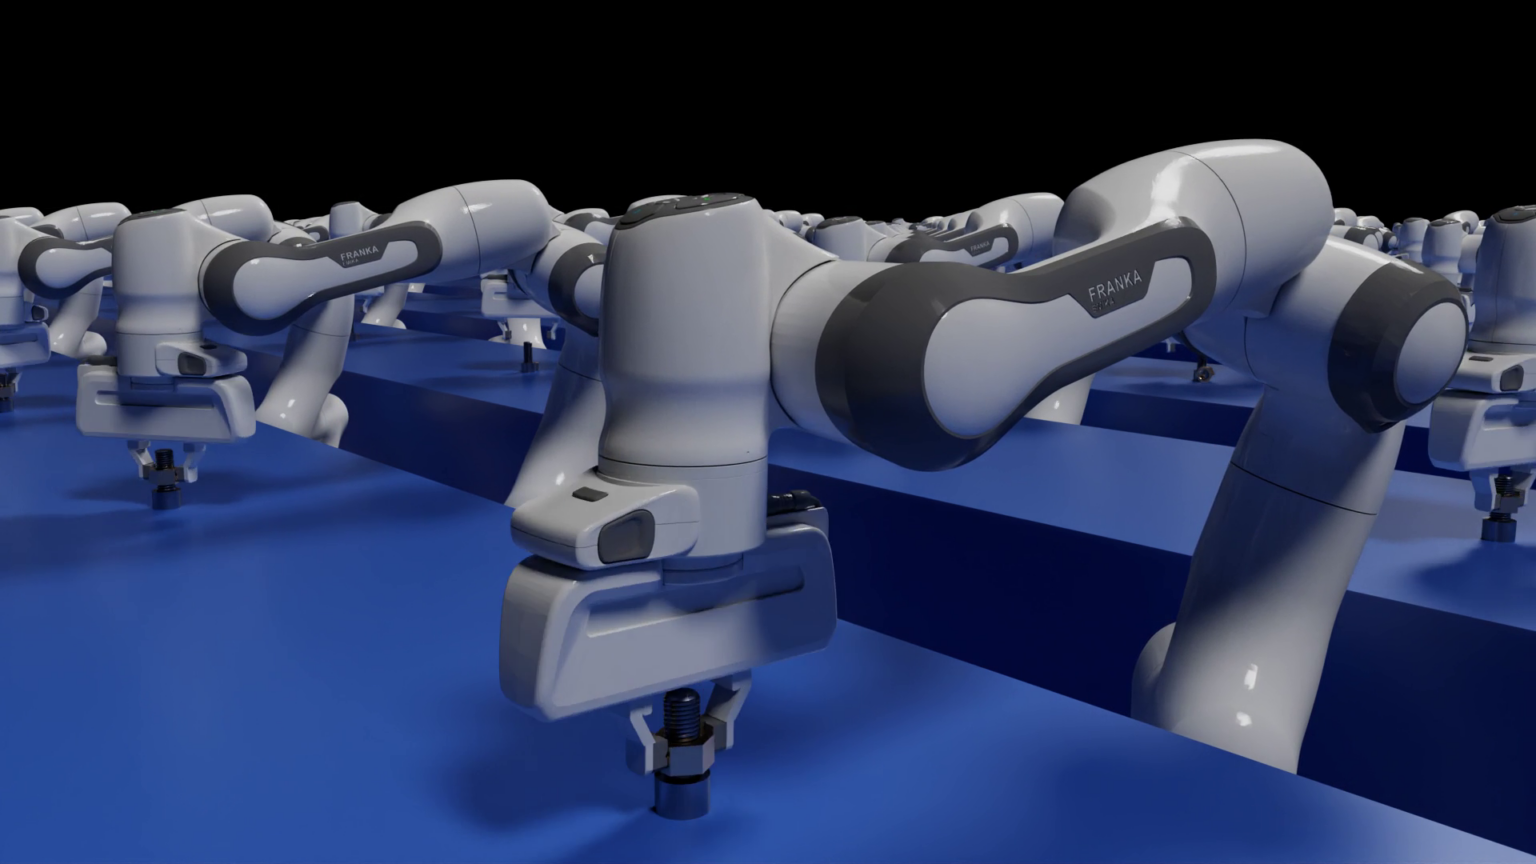
\includegraphics[width=\linewidth]{nvidia_isaac_gym.png}
        \caption{Parallel physics simulation (NVIDIA)- Sourced from the official \href{https://developer.nvidia.com/isaac/sim}{NVIDIA Isaac Sim} website}
        \label{fig:isaac-sim}
    \end{subfigure}
    \hfill
    \begin{subfigure}[b]{0.48\linewidth}
        \centering
        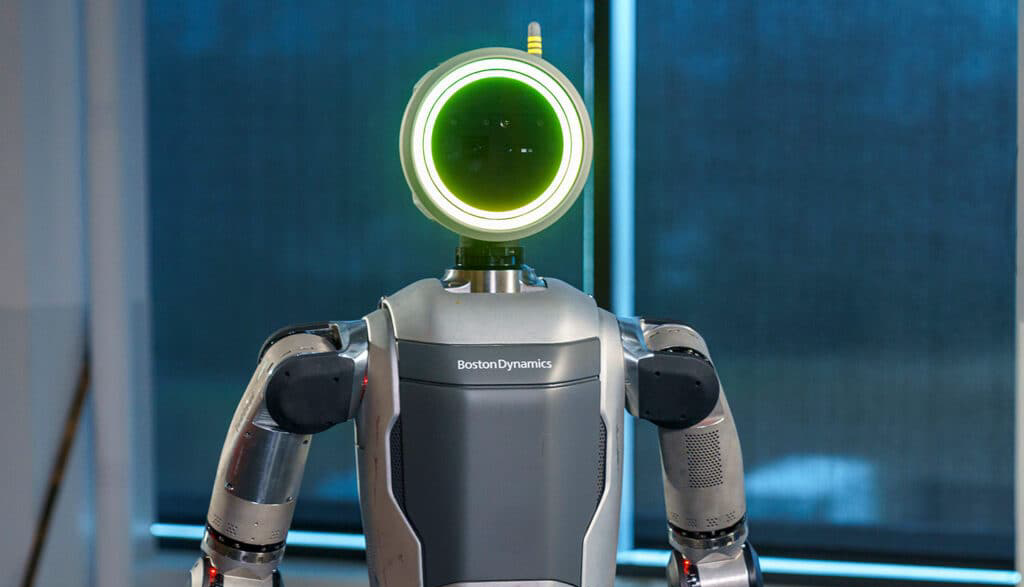
\includegraphics[width=\linewidth]{boston_dynamics_atlas.png}
        \caption{Embodied dynamic platform (Atlas) - Sourced from the official \href{https://bostondynamics.com/}{Boston Dynamics} website}
        \label{fig:boston-dynamics}
    \end{subfigure}

    \vspace{0.5em}

    \begin{subfigure}[b]{0.48\linewidth}
        \centering
        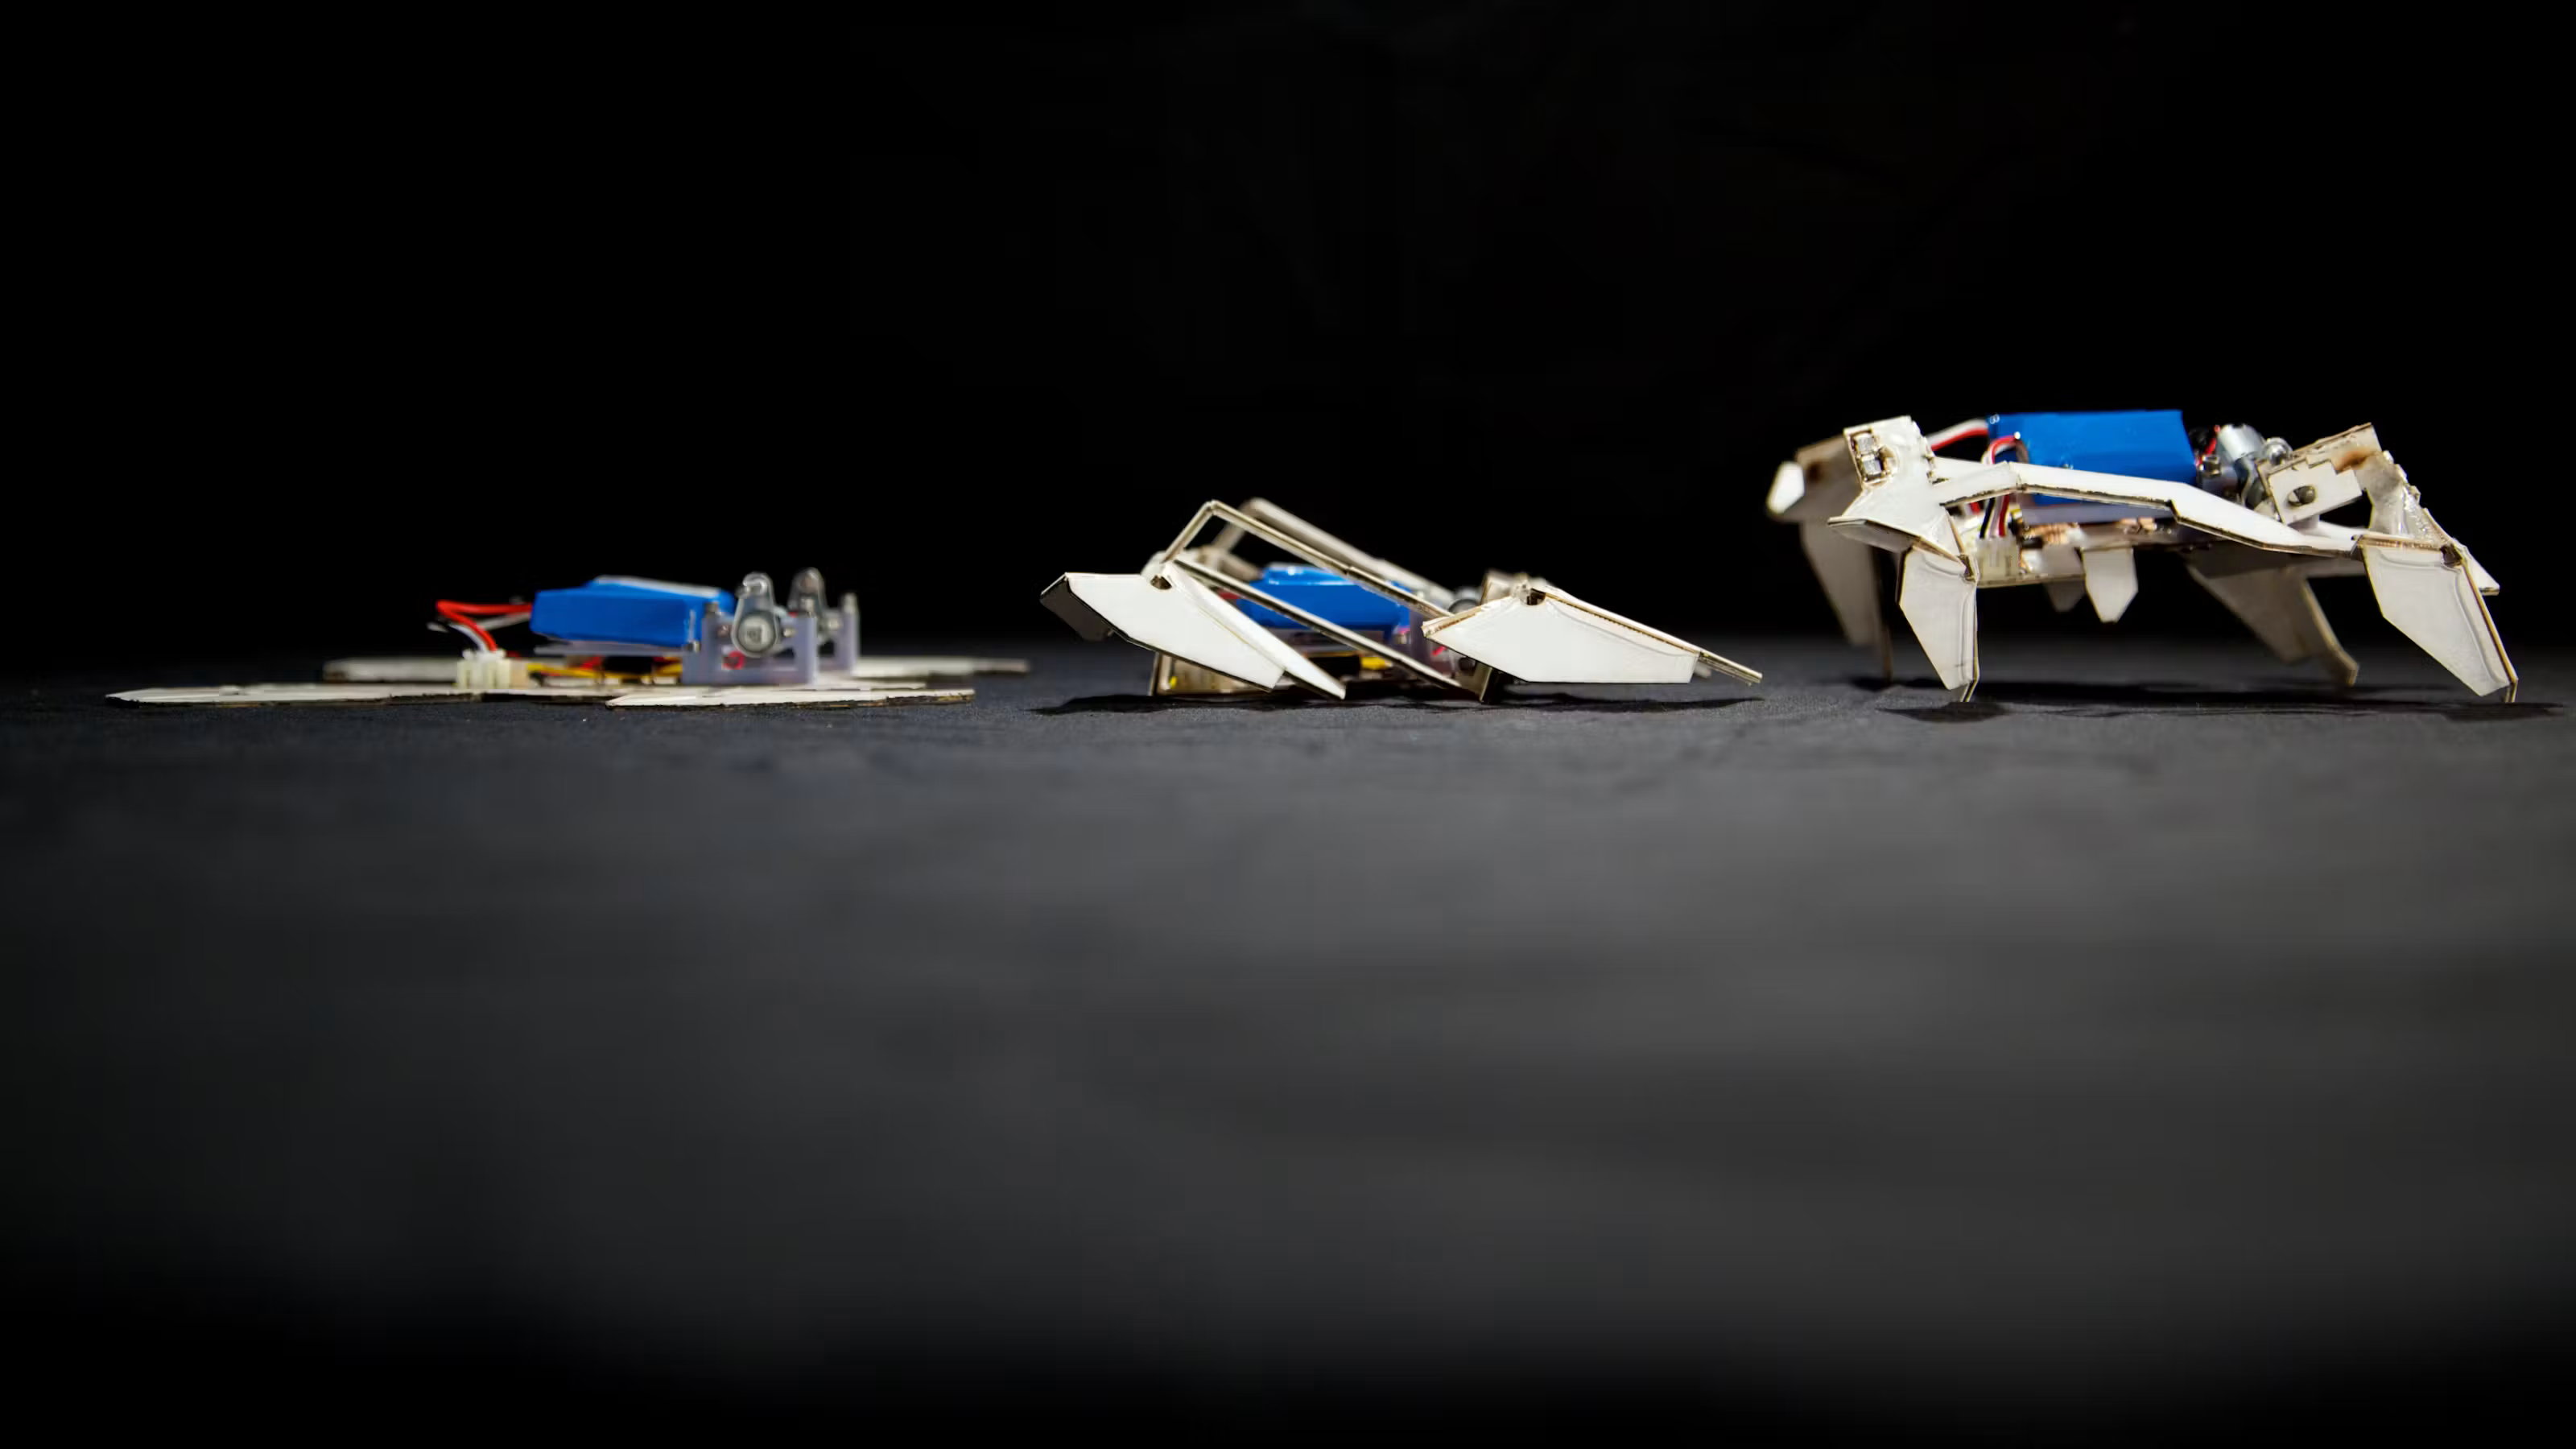
\includegraphics[width=\linewidth]{self_folding_robot.png}
        \caption{Planar 2D-to-3D self-folding mechanism - Sourced from the official \href{https://robotics.stanford.edu/}{Stanford Robotics} website}
        \label{fig:self-folding}
    \end{subfigure}
    \hfill
    \begin{subfigure}[b]{0.48\linewidth}
        \centering
        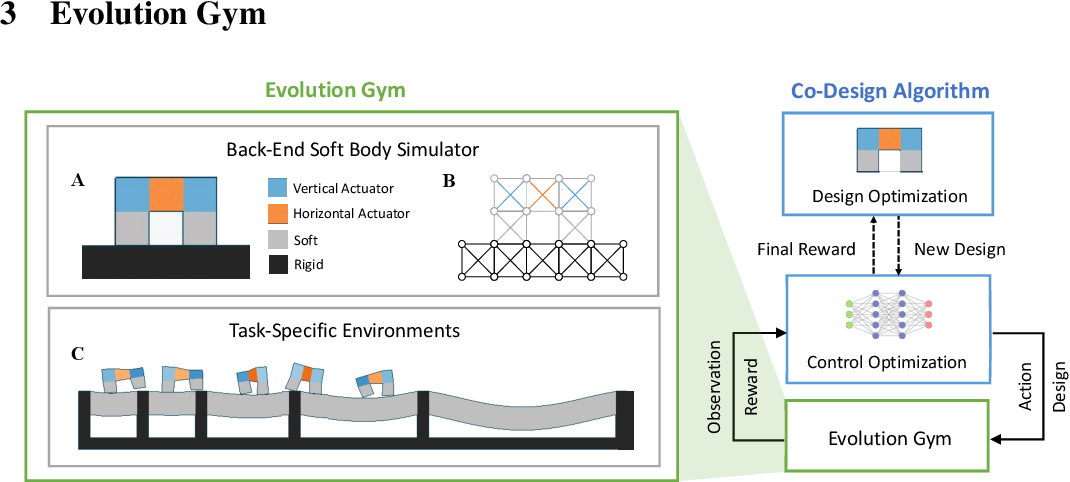
\includegraphics[width=\linewidth]{evolution_gym_codesign.png}
        \caption{Morphology-control co-design loop - Sourced from the official \href{https://www.csail.mit.edu/}{MIT CSAIL} website}
        \label{fig:evolution-gym}
    \end{subfigure}

    \caption{Key paradigms informing automated modular robot design: (a) parallelized GPU physics simulation; (b) dynamic hardware requiring body-brain integration; (c) planar-to-3D self-folding; (d) evolutionary co-design with policy learning \citep{bhatia2021evolution, li2023modular, yang2024machine}.}
    \label{fig:automated-design-hook}
\end{figure}



\subsection{The Roblet Platform}
Roblets are small, modular units with magnetic bonding sites and foldable sections. The units can be assembled from a two-dimensional arrangement and then folded into a three-dimensional robot. Locomotion is produced by an externally applied oscillating magnetic field rather than by motors placed in every module. This combination makes Roblets a useful test case for automated design because morphology affects assembly, folding, magnetic response and motion at the same time \citep{han2023roblets}.

\begin{figure}[H]
    \centering
    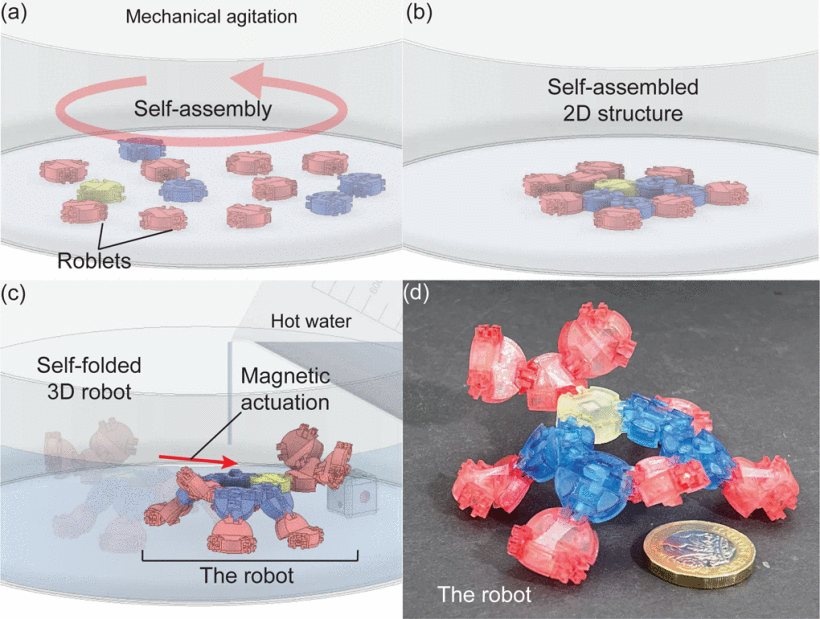
\includegraphics[width=0.6\linewidth]{roblet_paper_image_on_assembly_folding_actuation.png}
    \caption{Roblet assembly, folding and actuation: (a) magnetic 2D self-assembly, (b) heat-triggered 3D self-folding, (c) magnetically driven locomotion. Source: Han et al., IROS 2023 \citep{han2023roblets}.}
    \label{fig:roblet-assembly-folding-actuation}
\end{figure}

\subsection{Swarm Communication via Light-Based Virtual Pheromones}
Light-sensitive joints provide a simple local reaction primitive. A joint can respond to a one-sided light stimulus by changing the robot's turning behaviour, or to a wider stimulus by changing its speed. Light is used here as a simulatable stand-in for pheromone signalling, so a directional light source represents the cue a neighbouring robot's pheromone trail would otherwise provide. These responses are relevant to virtual pheromone communication because a robot could, in principle, move towards or away from a signal produced by another robot. In this project the primitive was evaluated on one simulated robot at a time. No multi-robot swarm simulation was carried out, so the results concern a building block of swarm behaviour rather than swarm coordination itself.


\section{Problem Statement}
Existing Roblet morphologies are designed by hand, which limits the range of structures that can be considered \citep{han2023roblets}. The difficulty is increased because a candidate is defined by interacting module types, port connections, module count, fold angles and light-response settings. Even before all graph connections are counted, allowing between 2 and 40 modules creates a large discrete search space.

The problem addressed in this report is the limited integration of morphology generation, self-folding behaviour and locomotion performance in an evolutionary robotic system. The central hypothesis is that an ML-assisted evolutionary framework can generate legal two-dimensional Roblet configurations, evaluate their folded three-dimensional behaviour and use the resulting measurements to improve the population. A second question is whether entropy-based folding complexity and light-response measures can reveal relationships between morphology and behaviour. The random-baseline comparison is used later to assess the selected ML mechanism; it is not the main hypothesis.

\section{Aims and Objectives}
The project aim was to develop an ML-assisted evolutionary framework within the Roblet platform for designing two-dimensional module morphologies that self-assemble, self-fold and locomote magnetically. The basic objectives were to: (O-1) develop a Python evolutionary approach for generating self-assembling configurations; (O-2) extend the simulation to support two-dimensional to three-dimensional self-folding; (O-3) evaluate folded structures under magnetic actuation and feed their fitness back into evolution; and (O-4) analyse evolved morphologies and their influence on locomotion across generations.

The original advanced objective AO-1 concerned comparing surrogate-learning methods for fitness prediction. It was changed during the project to the development of attractive and repulsive light-response objectives, since direct parallel simulation and caching made surrogate prediction less necessary and the reaction primitives were more closely related to the platform motivation. AO-2 remained the investigation of entropy and morphology complexity in relation to locomotion and evolutionary outcomes.

\section{Contributions}
The main contributions are as follows:
\begin{itemize}
    \item A graph-based Roblet genotype with symmetry construction and grammar-legal structural edits.
    \item A MuJoCo evaluation path from a two-dimensional graph to a folded, magnetically actuated three-dimensional assembly.
    \item A four-objective formulation combining locomotion, folding complexity and light-response behaviour, with separate attractive and repulsive runs.
    \item A PPO graph policy that selects mutation and crossover actions, together with a uniform-random comparison arm.
    \item Evaluation tools for convergence, hypervolume, Pareto structure, action use and RL training behaviour.
\end{itemize}
The intended contribution is the combination of policy-guided graph editing for both mutation and crossover with many-objective selection and Roblet-specific constraints, rather than discrete RL actions alone.

\section{Project Management}
The development and execution of this project were tracked against a structured 17-week schedule running from 15 May 2026 to 07 September 2026. Fig.~\ref{fig:gantt} shows the planned-versus-actual timeline for each phase; Table~\ref{tab:project_schedule} records the key technical outcome delivered in each.

\begin{table}[htbp]
\centering
\small
\caption{Key technical outcomes recorded for each project phase (Fig.~\ref{fig:gantt} gives the corresponding planned-versus-actual timeline).}
\label{tab:project_schedule}
\begin{tabular}{p{4.6cm} p{9.2cm}}
\hline
\textbf{Project Phase} & \textbf{Key Technical Outcomes} \\ \hline
Literature Review \& Background & Initial background review; extended through mid-July during formal review submission. \\
Simulation Framework \& Physics Engine & Self-folding XML setup, joint torque control, and oscillating magnetic actuation. \\
Morphology Representation & Directed graph serialization, visualizer interface, and port connection logic. \\
Evolutionary Framework Integration & EA pipeline initialization, grammar-masking collision gates, symmetry enforcement, and shape entropy. \\
ML-Assisted Optimisation (PPO / RL) & Pheromone response metrics, RL actor-critic integration, and action-penalty tuning. \\
Simulation Runs \& Analysis & Headless parallel simulations, magnetic sweep optimization, and convergence plotting. \\
Dissertation Writing \& Revision & Final thesis compilation, manuscript drafting, and algorithmic bug fixes. \\ \hline
\end{tabular}
\end{table}

\begin{figure}[H]
\centering
\begin{ganttchart}[
    hgrid,
    vgrid,
    x unit=0.42cm,
    y unit chart=0.55cm,
    y unit title=0.6cm,
    bar height=0.55,
    bar label font=\scriptsize,
    title label font=\scriptsize,
]{1}{17}
\gantttitle{Week number from project start (15 May 2026)}{17}\\
\gantttitlelist{1,...,17}{1}\\
\ganttbar{Literature Review -- planned}{1}{4}\\
\ganttbar{Literature Review -- actual}{1}{11}\\
\ganttbar{Simulation Framework -- planned}{5}{6}\\
\ganttbar{Simulation Framework -- actual}{7}{11}\\
\ganttbar{Morphology Representation -- planned}{7}{8}\\
\ganttbar{Morphology Representation -- actual}{9}{12}\\
\ganttbar{Evolutionary Framework Integration -- planned}{9}{10}\\
\ganttbar{Evolutionary Framework Integration -- actual}{12}{15}\\
\ganttbar{ML-Assisted Optimisation -- planned}{13}{14}\\
\ganttbar{ML-Assisted Optimisation -- actual}{15}{16}\\
\ganttbar{Simulation Runs \& Analysis -- planned}{14}{16}\\
\ganttbar{Simulation Runs \& Analysis -- actual}{13}{16}\\
\ganttbar{Dissertation Writing -- planned}{14}{17}\\
\ganttbar{Dissertation Writing -- actual}{15}{17}\\
\end{ganttchart}
\caption{Revised Gantt chart of planned versus actual project progress, by week number from the project start date (15 May 2026); see Table~\ref{tab:project_schedule} for exact dates.}
\label{fig:gantt}
\end{figure}

Initial development proceeded on schedule, with foundational XML generation and hinge self-folding mechanisms established in early July. However, actual progress diverged from the baseline plan across key technical phases:

\textbf{Simulation Framework Bottlenecks and Downstream Schedule Shifts:}
Building the physics simulation environment and dynamic assembly generator consumed nearly four weeks of intensive development (from early July through late July), significantly longer than the planned two-week allocation. Debugging low-level physical dynamics—such as hinge joint flapping, accurate module spatial layout in XML, connector inertial mass adjustments for embedded magnets, dynamic torque actuation under oscillating magnetic fields, and fluid/glass interactions, required extensive iteration across dozens of code refinements. Because multi-objective optimization (MOO) and reinforcement learning (RL) both rely on a stable, bug-free physics evaluator, downstream framework integration was intentionally held back until high-fidelity simulation and headless parallel execution were completely validated in mid-August.

\textbf{Pivot from ML Surrogate Fitness to Direct Pheromone Metrics (AO-1 Adjustment):}
The original project objectives specified training a machine learning surrogate model to predict physical locomotion fitness to accelerate evolutionary search. During mid-August, when headless parallel MuJoCo simulations achieved high throughput (around 1.2 minutes per generation), surrogate fitness prediction was deemed unnecessary. Instead, the advanced objective was pivoted toward implementing direct light-response and virtual pheromone attraction/repulsion behavior metrics. This modification aligned the physics-in-the-loop pipeline with high-fidelity behavioral evaluation without relying on surrogate approximations.

\textbf{Delayed RL Integration and Redesign Phase:}
While evolutionary pipeline integration was scheduled for late July, establishing stable multi-objective constraints (collision checks, mirror symmetry, and shape entropy) extended through mid-August. Consequently, the implementation of the PPO actor-critic network for RL-guided graph edits commenced later than planned, in late August. Initial diagnostic runs revealed policy collapse caused by excessively severe penalties on invalid grammar actions and elitism handling issues in NSGA-III. Reallocating contingency time in late August enabled targeted redesign of penalty structures and operator selection routines, successfully stabilizing the actor-critic policy before final thesis compilation.

\section{Dissertation Structure}
Chapter 3 develops the methodology in two parts: Section 3.1 describes the Roblet platform and its physics-in-the-loop MuJoCo simulation, while Section 3.2 describes the graph genotype, the multi-objective fitness formulation, and the evolutionary optimisation and PPO-guided learning process built on top of that simulator, ending with the computational pipeline, configuration, baseline arm and evaluation metrics. Chapter 4 presents convergence, trade-offs, morphology and RL-versus-baseline results together with RL diagnostics. Chapter 5 discusses these findings against the objectives set out in this chapter. Chapter 6 closes with the delivered contributions, limitations and future work.


\chapter{Literature Review}
Designing autonomous modular robots requires addressing both physical mechanics and algorithmic optimization. Historically, creating functional robot morphologies depended heavily on human engineering intuition, a process that inherently restricts exploration to familiar configurations. To overcome this, the automated design of self-assembling and self-folding modular robots demands a synthesis of physical hardware platforms, evolutionary multi-objective optimization, graph-structured representations, and reinforcement learning.

This literature review evaluates the foundational frameworks and recent advances across seven domain areas. Section 2.1 surveys the landscape of modular and self-reconfigurable robots, positioning the unique physical traits of Roblets relative to existing hardware systems. Section 2.2 examines automated robot design as a broader design-automation problem, including generative and grammar-based structural representations. Section 2.3 reviews how AI and machine learning techniques are used to guide that design search. Section 2.4 turns to evolutionary robotics and morphology-control co-design, focusing on structural representation and search-space management. Section 2.5 critically evaluates reinforcement learning techniques applied to structural search versus control optimization. Section 2.6 analyzes multi-objective evolutionary algorithms, focusing on high-dimensional Pareto optimization. Section 2.7 reviews graph-structured representations and graph neural network policies for variable-morphology systems. Finally, Section 2.8 synthesizes these findings to define the precise research gap addressed in this work.

\section{Modular and Self-Reconfigurable Robots}
Modular robotic systems build functional machines by combining standardized physical building blocks. The foundational principles of programmable self-assembly established by Klavins (2007) showed how complex structures could emerge from simple units governed by local bonding rules \citep{4272328}. Survey work on evolutionary modular robotics identifies the resulting design-space problem: as the number of interfaces and possible assemblies increases, hand-crafting effective topologies becomes difficult and computational search becomes increasingly important \citep{alattas2019evolutionary}.

The Roblet platform (Han et al., 2023) provides a distinctive case within modular robotics. A Roblet begins as a flat, 2D-printed unit with magnetic bonding interfaces; heat-responsive PVC hinges transform the assembled sheet into a 3D structure, and an externally oscillating magnetic field drives locomotion. Light-sensitive joints additionally provide a route to virtual-pheromone reaction primitives. Despite these capabilities, the Roblet configurations reported in prior work remain hand-designed, making them a suitable test case for automated co-design of topology, folding and behaviour \citep{han2023roblets}.

\section{Automated Robot Design and Modularity}
Automated robot design addresses the limits of manual robot engineering, which remains difficult because robot performance depends on tightly coupled interactions among body structure, sensing, actuation and behaviour \citep{matthews2023efficient,park2021computational}. In modular robotics, this problem is often tackled by representing robots as assemblies of reusable units whose topologies and parameters can be optimized automatically rather than redesigned from scratch for each task \citep{li2023modular,hu2022modular}. Generative and grammar-based approaches make this design space more tractable by exploiting modularity, hierarchy and rule-based graph representations that can encode large numbers of fabricable morphologies \citep{hornby2003generative,zhao2020robogrammar}. Survey work therefore treats modularity as both a hardware strategy and a computational abstraction for design automation, because its discrete structure can simplify search and support reconfiguration and reuse \citep{li2023modular,alattas2019evolutionary}.

\section{AI and ML in Automated Robot Design}
AI and machine learning are increasingly used to bias robot design search toward promising candidates rather than relying on exhaustive combinatorial exploration \citep{qiu2024robomorph,11003187}. Reinforcement learning has been used not only to evaluate candidate bodies through learned control, but also to guide modular design as a sequential decision-making process in which robots are assembled incrementally \citep{qiu2024robomorph,park2021computational}. Generative models broaden this further: GAN-based methods learn one-to-many mappings from task to diverse feasible modular designs, which is useful when several morphologies perform similarly well \citep{hu2022modular}. Recent LLM-based frameworks extend this trend by acting as generative operators inside evolutionary loops, while broader commentary suggests LLMs can also support conceptual and technical stages of robot design through human--AI co-design \citep{qiu2024robomorph,stella2023can}.

\section{Evolutionary Robotics and Morphology-Control Co-Design}
Evolutionary Robotics (ER) applies the principles of natural selection to simultaneously synthesize a robot's physical morphology (body) and controller (brain). A broad survey of modular design automation (Li et al., 2023) categorizes the field into three core challenges: representation (genotype-to-phenotype mapping), search space exploration, and controller-morphology co-optimization \citep{li2023modular}.

A central challenge in evolving modular structures is managing a large, constrained design space. Work on evolutionary robot design also considers interactions among design variables, including epistatic effects, while Evolution Gym highlights the importance of expressive design representations and the difficulty of co-optimizing body structure and control as the search space grows \citep{miras2026epistatic,bhatia2021evolution}. In this project, grammar masking is introduced as a method contribution: it enforces topological and kinematic constraints, such as valid port adjacency, before a candidate is sent to physics simulation. This implementation choice is intended to reduce evaluations of plainly illegal designs; it is not presented as an established conclusion of the cited literature.

In terms of structural representation, graph-based heuristic search methods (Xu et al., 2021) provide one example of modeling robot topologies for design search \citep{xu2021multi}. Representing robot bodies as directed graphs allows evolutionary operators to operate on discrete subtrees. However, evaluating candidate morphologies presents a computational bottleneck. Benchmark platforms such as Evolution Gym (Bhatia et al., 2021) provide standardized grid/voxel-based soft-robot environments for large-scale evaluation \citep{bhatia2021evolution}. While useful for general algorithm comparison, generic voxel benchmarks do not capture all of the specific physical constraints of Roblets, such as planar 2D-to-3D self-folding kinematics, magnetic field actuation, and directional light-sensing responses. Consequently, a dedicated, physics-in-the-loop simulation environment grounded in MuJoCo is necessary to evaluate Roblet candidate designs against real-world physical dynamics.

\section{Reinforcement Learning for Robot Design}
Reinforcement Learning (RL) is widely used to learn control policies for existing robot bodies, including in micro- and nanorobotics \citep{yang2024machine}. By contrast, morphology-control co-design remains a computationally demanding problem: surveys and co-design studies identify the interaction between body and controller search as a central challenge, while Evolution Gym notes that combining design optimization with deep RL remains difficult in harder environments \citep{li2023modular,sun2023co,bhatia2021evolution}.

Applying RL to structural design can therefore involve discrete design decisions in addition to continuous control. The cited literature includes RL-based morphology decisions and joint morphology-control optimization, but it does not establish PPO graph-edit actions as a standard alternative to other EA-RL hybrids \citep{li2024reinforcement,sun2023co,li2024bridging}. The present thesis uses PPO to select structural actions within an evolutionary loop; this is the design being evaluated here, rather than a capability claimed for the cited studies.

Hybrid frameworks combining Evolutionary Algorithms (EAs) and RL are consequently relevant to this problem. Across the cited work, EAs commonly provide population-based morphology search while RL learns or refines behaviour, although the division of labour varies between methods \citep{li2023modular,sun2023co,li2024bridging}. Other work uses RL-inspired signals to inform evolutionary operator choices, illustrating that hybridisation need not mean that an RL policy directly performs every structural edit \citep{brown2025reinforcement}.

The approach developed in this thesis uses a Proximal Policy Optimization (PPO) agent to select structural actions, such as node additions, subtree prunings, and crossover subtree swaps, on candidate graph genotypes inside an active evolutionary loop. Within the supplied corpus, this appears distinct from the cited co-design baselines because those sources do not directly test PPO over graph mutations and crossover. The distinction is therefore a positioning of the present method, not a claim that all prior body-brain co-design methods restrict RL to motor control.

\section{Multi-Objective Evolutionary Algorithms in Robotics}
Real-world robot design inherently involves balancing conflicting performance requirements. A morphology optimized purely for forward locomotion speed often exhibits poor stability or excessive structural complexity. Multi-Objective Evolutionary Algorithms (MOEAs) address this by discovering a Pareto front, a set of non-dominated solutions representing optimal trade-offs between competing criteria.

Standard multi-objective algorithms, such as NSGA-II, rely on crowding distance metrics to maintain population diversity along the Pareto front. However, when the optimization problem involves more than three objectives (many-objective optimization), crowding distance metrics lose selectivity because almost all individuals become non-dominated relative to one another. To resolve this, Deb and Jain (2014) developed NSGA-III, which replaces crowding-distance sorting with reference-direction-based niching \citep{deb2014evolutionary}. By projecting candidate solutions onto uniformly distributed reference lines in objective space, NSGA-III maintains high population diversity and convergence pressure across higher-dimensional trade-off surfaces.

In robotic co-design, integrating machine learning with MOEAs is relevant when the design space is constrained. Ming et al. (2024) provides a related example of deep reinforcement learning selecting genetic operators in constrained multi-objective optimization \citep{ming2024constrained}. This project applies NSGA-III to a four-objective optimization landscape:
\begin{enumerate}
    \item Maximize folded-gait locomotion velocity ($f_1$),
    \item Maximize entropy-based folding complexity gain ($\Delta H = H_{\text{3D}} - H_{\text{2D}}$) ($f_2$),
    \item Maximize/minimize light-based pheromone yaw response ($f_3$),
    \item Maximize/minimize light-based pheromone speed response ($f_4$).
\end{enumerate}
NSGA-III is well-justified for this many-objective setting because its reference-direction niching is designed to maintain diversity and selection pressure when several objectives make ordinary crowding-based selection less discriminating \citep{deb2014evolutionary}.

\section{Graph-Structured Policies for Variable Morphology}
A persistent challenge in evolving variable modular architectures is learning across candidates that differ in node counts, degrees of freedom, and topological layouts. Variable morphologies create changing dynamics and state-action distributions, which complicate shared learning across designs \citep{sun2023co,li2023modular}.

Graph-based policies appear promising for variable-morphology settings because they can represent relationships between modules and connections directly. Existing work in the supplied corpus also uses graph-based search for robot design and morphology-aware or morphology-agnostic policy learning \citep{xu2021multi,luo2025gcnt,wang2019neural,wang2026evolving}. These sources do not establish a single standard graph-policy architecture or directly document the particular attention and operator details used in this thesis.

These studies motivate morphology-aware representations, while leaving open how a policy should select legal graph edits within an evolutionary search loop. This thesis addresses that narrower design question with a graph encoder and PPO policy. The broader literature also includes studies of adaptive or life-like behaviour in flexible and active structures, which reinforces the value of evaluating morphology together with behaviour rather than treating shape as an isolated variable \citep{wei2026life}.

This work makes two implementation choices beyond the cited representations:
\begin{enumerate}
    \item \textbf{Per-Edge Multi-Head Attention:} A dedicated Graph Transformer encoder with multi-head attention per edge is used to capture directional flow and structural dependencies across Roblet connection ports.
    \item \textbf{Unified Structural Edit Policy:} Rather than using graph policies strictly to produce motor control torques, the Continuously-trained PPO agent uses the Graph Transformer encoder to directly output probability distributions over discrete structural edits (mutation and crossover subtree operations) across arbitrarily sized modular genotypes.
\end{enumerate}

\section{Summary and Research Gap}
While substantial progress has been achieved in modular robotics, evolutionary algorithms, and reinforcement learning, existing methodologies remain fragmented across these domains:
\begin{itemize}
    \item Modular platforms like Roblets (Han et al., 2023) offer compelling mechanical properties, such as heat-driven 2D-to-3D self-folding and external magnetic actuation, but their design space remains limited by manual human engineering \citep{han2023roblets}.
    \item The supplied co-design literature supports a distinction between RL for control and evolutionary search over design, but does not establish a direct robot-morphology example of PPO choosing graph-edit mutations and crossover.
    \item The cited sources motivate combining learned decision-making with evolutionary and many-objective search, while the particular integration of PPO-selected graph edits, NSGA-III and Roblet-specific constraints is the method evaluated in this thesis.
\end{itemize}

\textbf{Research Gap Statement:}
Within the supplied corpus, no directly comparable study is identified that combines (a) policy-guided evolutionary graph editing for both structural mutation and crossover, (b) high-dimensional (4-objective) NSGA-III Pareto search, and (c) domain-specific kinematic, folding, and light-response grammar constraints within a unified, physics-in-the-loop co-design pipeline. This corpus-bounded gap motivates the method developed in the following chapters; it is not an exhaustive claim about all prior work.

The following chapters detail the methodology developed to address this gap, presenting an automated evolutionary framework capable of discovering functional, highly non-intuitive Roblet morphologies.


\chapter{Methodology}
\label{ch:methodology}
This chapter describes how morphology, folding and locomotion are modelled and optimised. Section~\ref{sec:sim-framework} presents the physical Roblet platform and its physics-in-the-loop MuJoCo simulation, establishing what is simulated and how fitness is measured from it. Section~\ref{sec:evo-learning} then describes the evolutionary search and learning process built on top of that simulator: the graph genotype and grammar, the multi-objective fitness formulation, the PPO-guided actor-critic, NSGA-III selection, and the resulting computational pipeline, configuration, baseline arm and evaluation metrics.

\section{The Roblet Platform and Physics Simulation}
\label{sec:sim-framework}

\subsection{Physical Roblet Hardware}
\begin{figure}[H]
    \centering
    \begin{subfigure}[b]{0.48\linewidth}
        \centering
        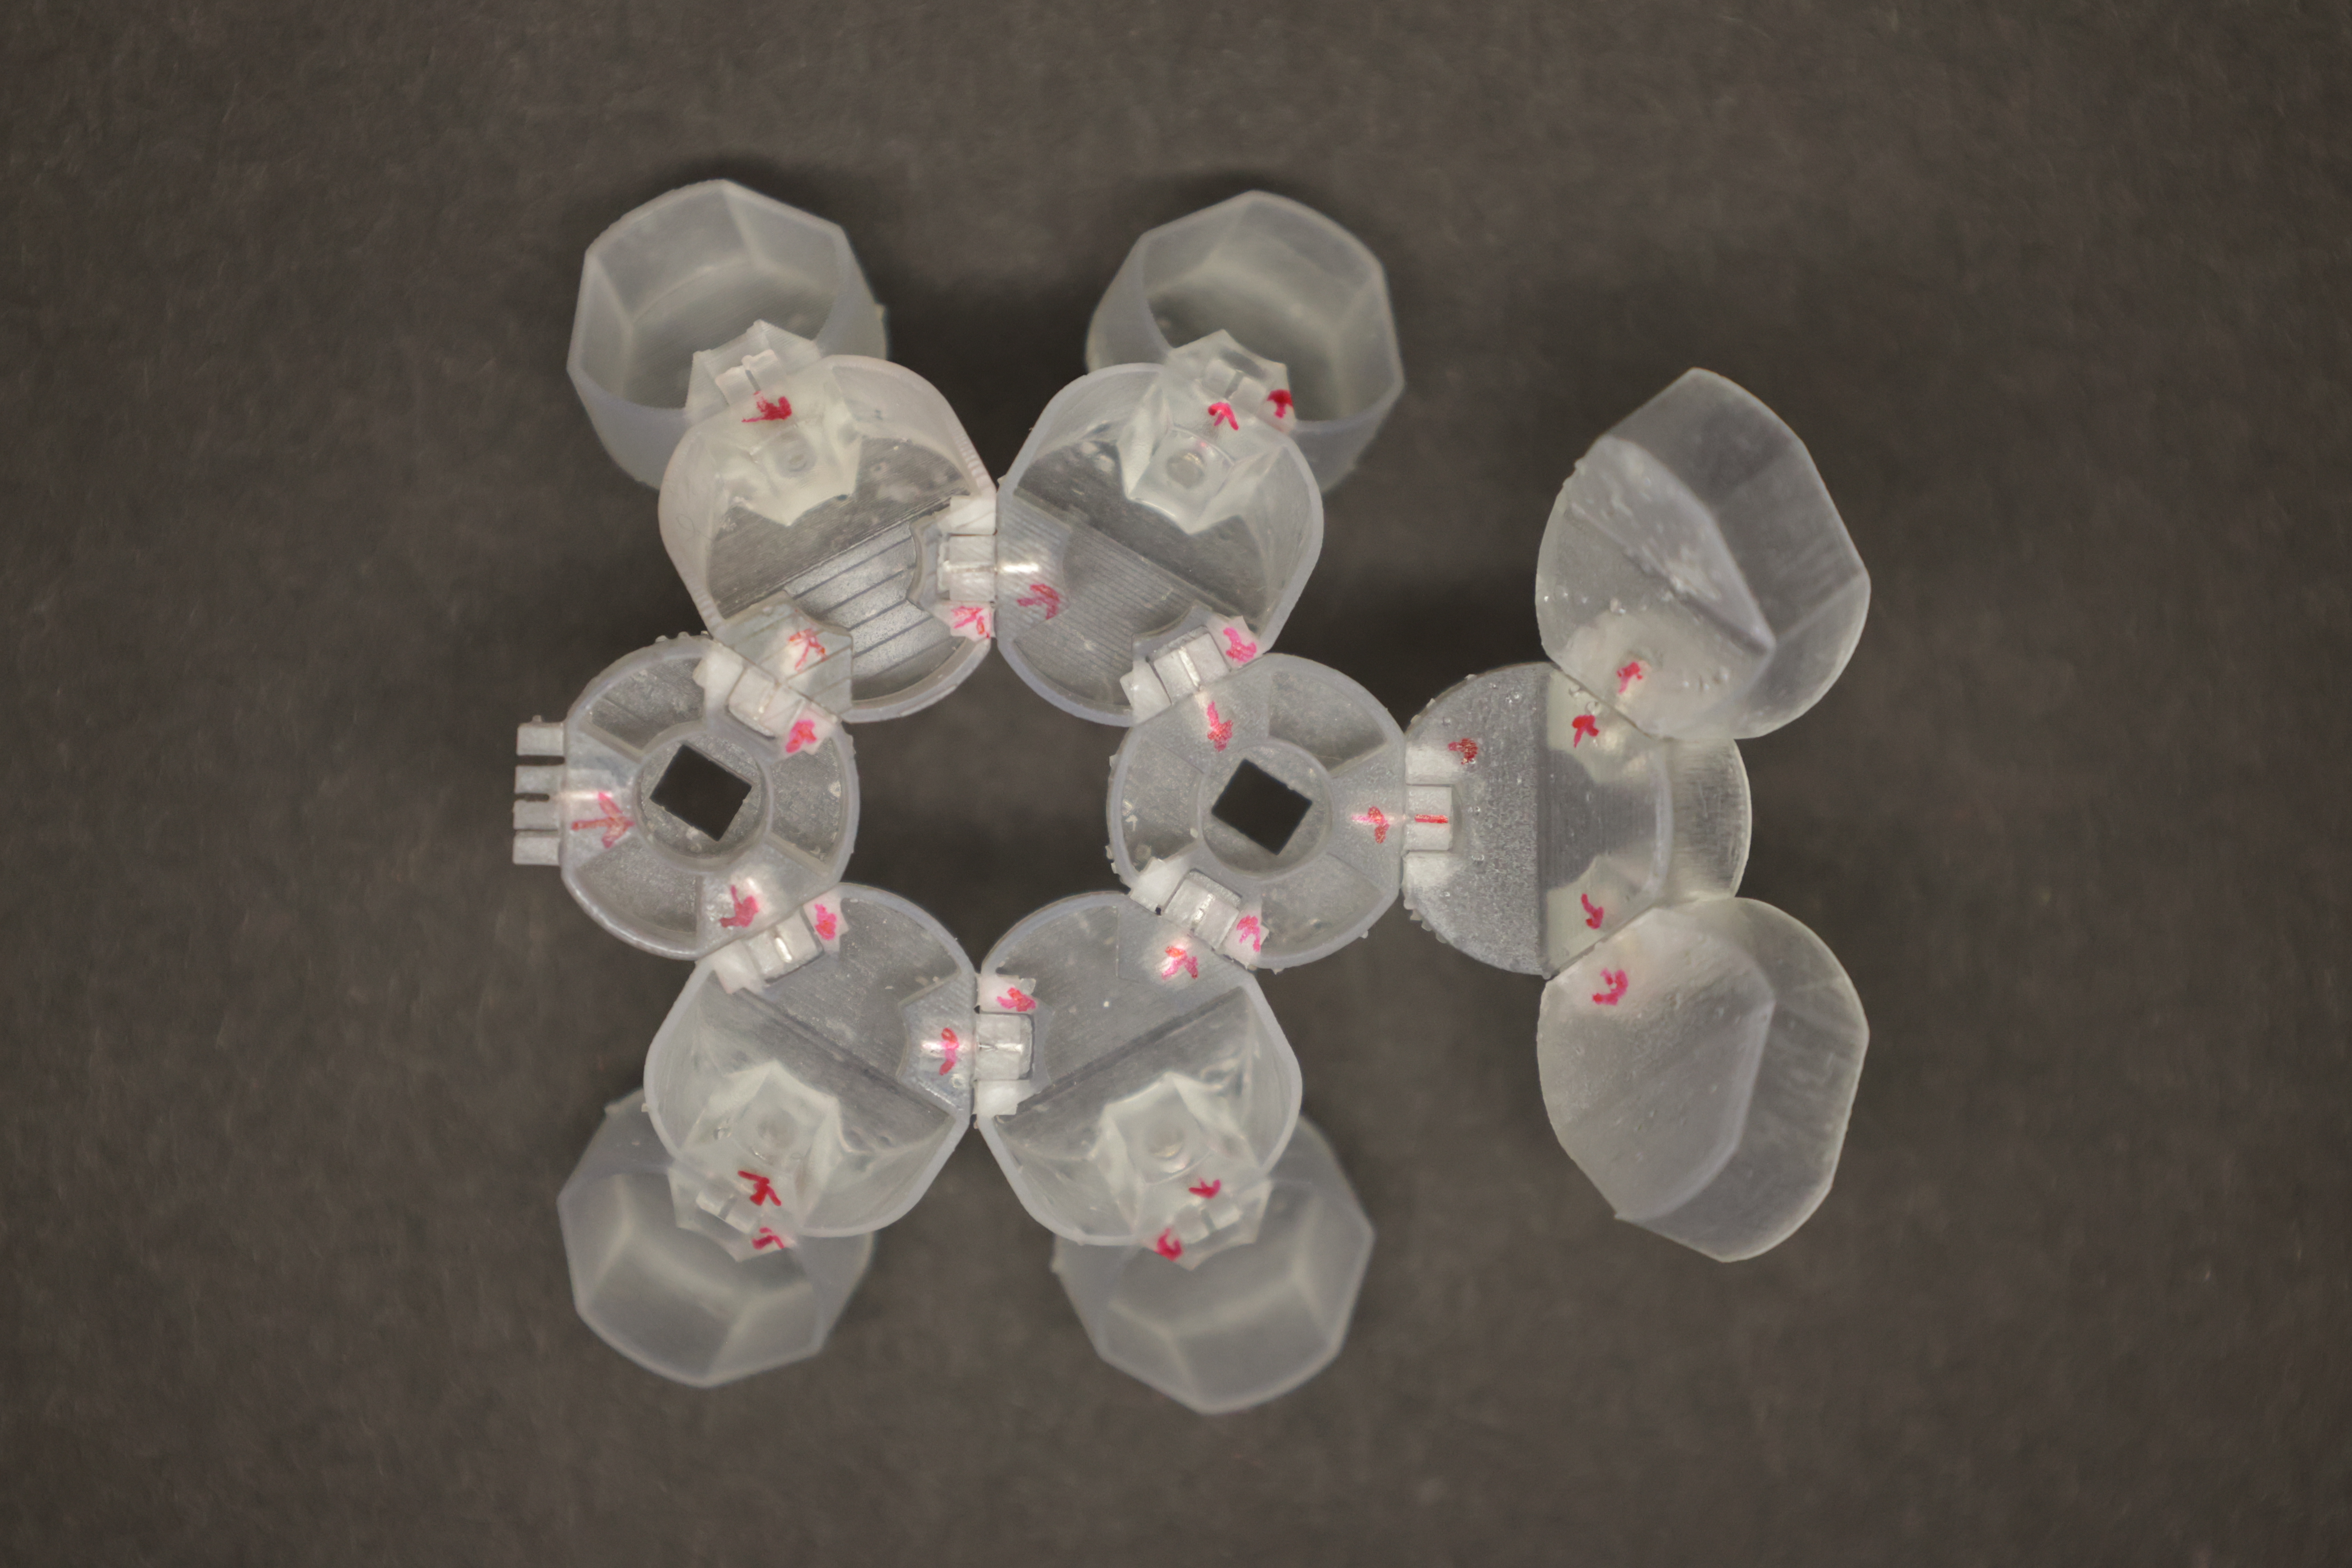
\includegraphics[width=\linewidth]{real_setup_topview.JPG}
        \caption{Top view.}
        \label{fig:real-setup-top}
    \end{subfigure}
    \hfill
    \begin{subfigure}[b]{0.48\linewidth}
        \centering
        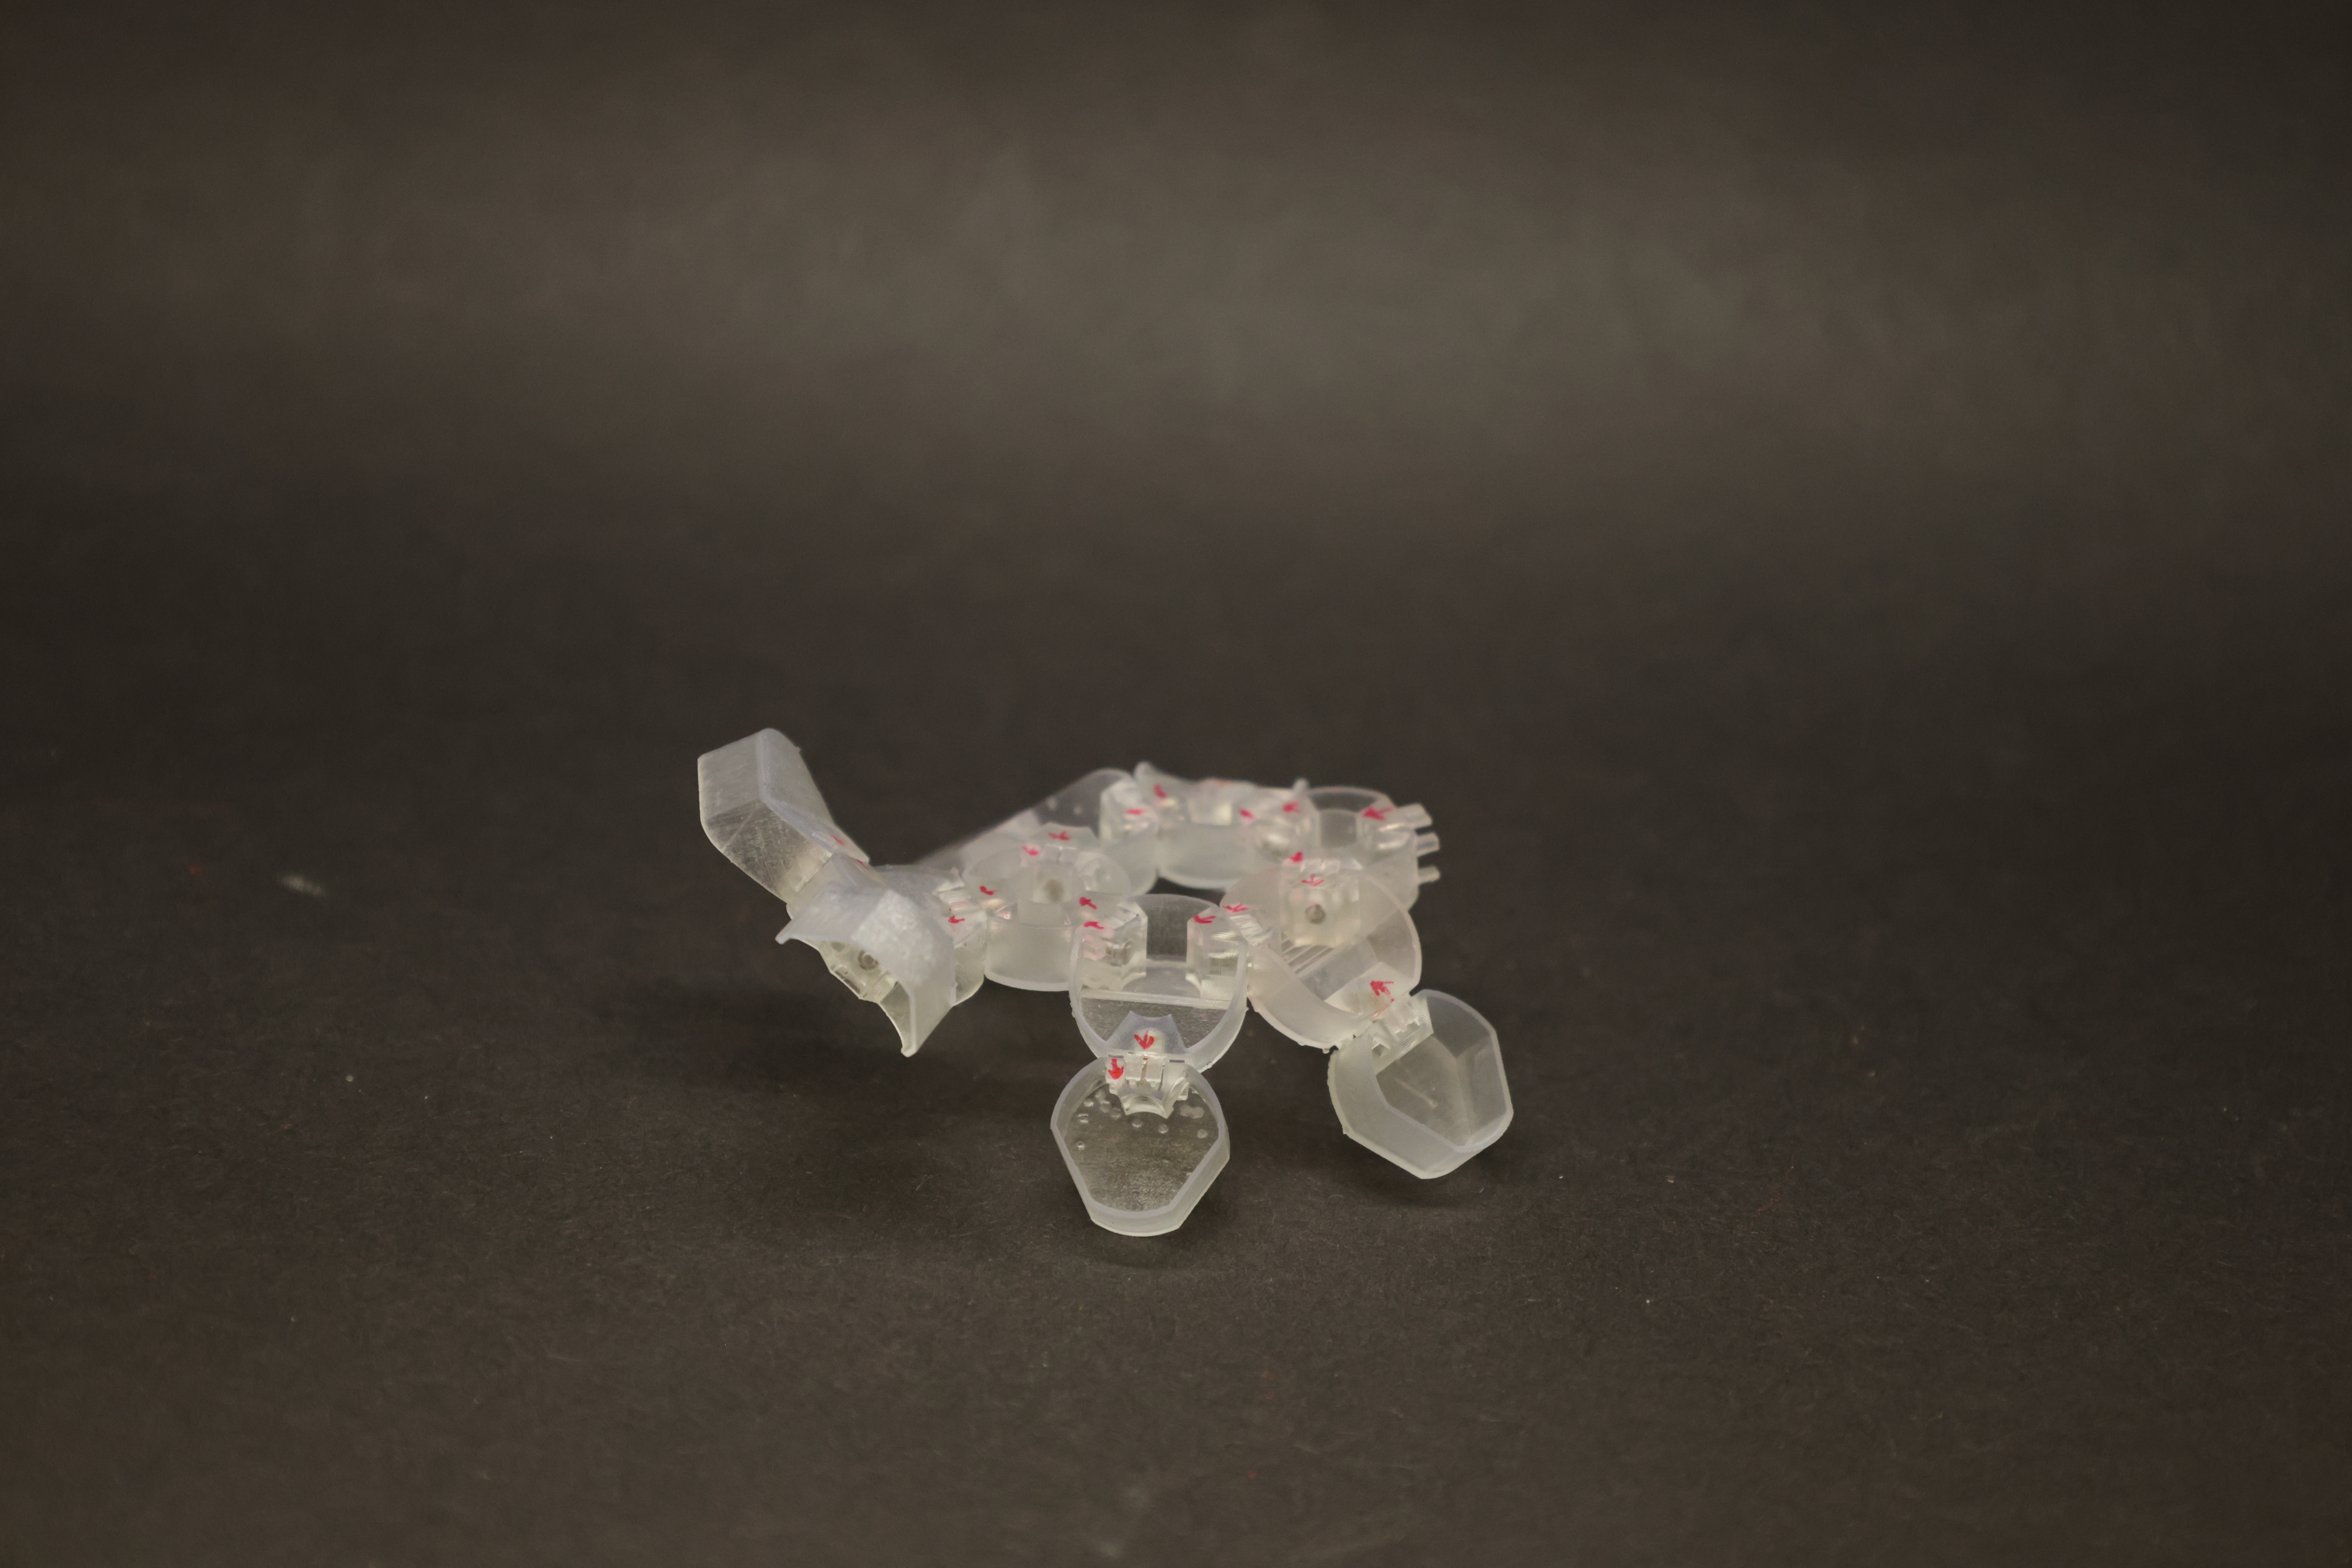
\includegraphics[width=\linewidth]{real_setup_sideview.jpg}
        \caption{Side view.}
        \label{fig:real-setup-side}
    \end{subfigure}

    \caption{Physical Roblet modules under macro-photography, showing translucent 3D-printed bodies with embedded magnets and port-orientation marks. Photograph by the Miyashita Lab \citep{han2023roblets}; compare with the digital twin (Fig.~\ref{fig:sim-setup}).}
    \label{fig:real-setup}
\end{figure}

\subsection{Actuation and Self-Folding Principles}
The physical design uses heat-responsive PVC hinges to convert the flat arrangement into a folded structure. In the simulation, this process is represented by allowing connected module bodies to settle into their folded configuration rather than prescribing the final pose directly. The assembled robot is then driven by an oscillating magnetic field. Each embedded magnet experiences a torque that depends on the field direction, and the combined torques produce the motion of the whole assembly.

The light-response mechanism is represented as a change at selected foldable joints. A one-sided stimulus is used to measure yaw response, while a wider stimulus is used to measure speed response. These two measurements form the reaction primitives used later in the evolutionary objective set. The simulator therefore provides a common route from morphology to folding, actuation and measurable behaviour.

\subsection{MuJoCo Digital-Twin Simulation}
\label{sec:digital-twin}
\begin{figure}[H]
    \centering
    \begin{subfigure}[b]{0.47\linewidth}
        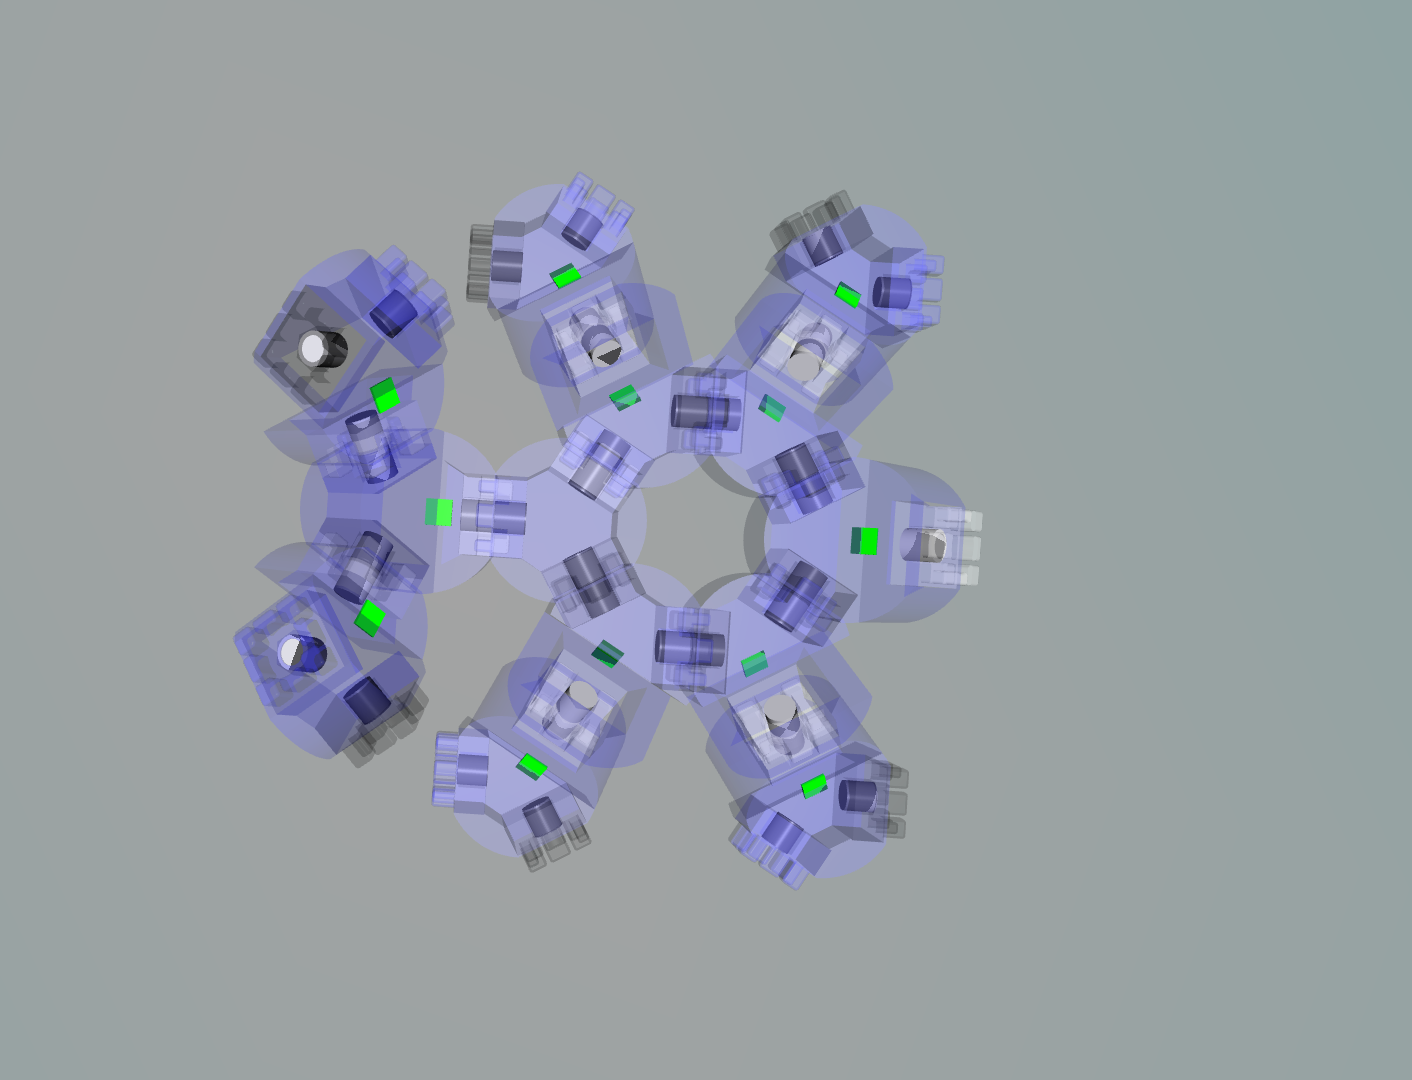
\includegraphics[width=\linewidth]{sim_setup_transparent.png}
        \caption{Top view, transparent bodies showing embedded magnets}
        \label{fig:sim-setup-transparent}
    \end{subfigure}
    \hfill
    \begin{subfigure}[b]{0.47\linewidth}
        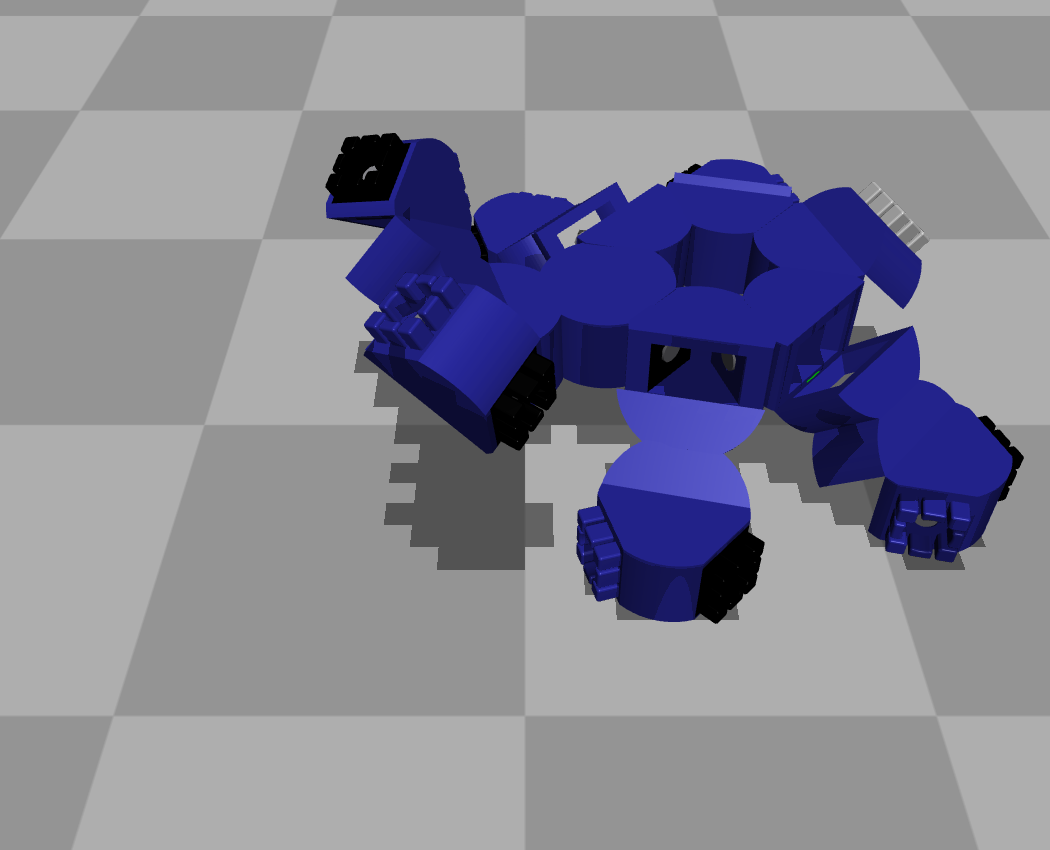
\includegraphics[width=\linewidth]{sim_setup.png}
        \caption{Rendered assembly}
        \label{fig:sim-setup-render}
    \end{subfigure}
    \caption{Simulated Roblet digital twin in MuJoCo, corresponding to Fig.~\ref{fig:real-setup}: (a) transparent top view verifying magnet placement, (b) rendered assembly.}
    \label{fig:sim-setup}
\end{figure}

The digital twin was implemented as a set of independent module bodies with mass, centre-of-mass and inertia values taken from Fusion 360 CAD mass-property exports for each of the six moulded part types (fold-hinge base, fold-hinge link, rigid body, and three connector variants). A cylindrical N42SH magnet model with magnetic moment $m=6.5\times10^{-3}\,\mathrm{A\,m^2}$ was placed at each connector. Connected bodies were joined with weld equality constraints. This choice allows the bodies to remain separate physical objects while their assembled relationship is enforced during settling; it is closer to the assembly process than a purely scripted kinematic tree.

The external field applies the torque $\boldsymbol{\tau}=\mathbf{m}\times\mathbf{B}$ to each magnet. For locomotion, candidate field strengths of $0.001$, $0.008$ and $0.025$ T were tested. The field was swept for each morphology because a small or heavy structure may stall at a field that drives another structure into excessive rolling or tumbling. The candidate with the highest stable velocity was retained.

\subsection{Simulation Parameters and Reproducibility}
\label{sec:sim-params}
The physical fidelity of the digital twin, and hence the reproducibility of any result in Chapters~\ref{ch:results}--\ref{ch:discussion}, depends on a set of environmental and material parameters that are fixed across every evolutionary run. Table~\ref{tab:sim-params} summarises the values needed to reproduce the physics simulation environment described above. The full per-part mass, inertia and geometry data, the exact software versions, and step-by-step setup instructions are given in Appendix~\ref{app:reproduce}.

\begin{table}[htbp]
\centering
\footnotesize
\caption{Key MuJoCo simulation parameters used to produce the results reported in this thesis. All values are taken directly from the simulator source and MJCF generator; MuJoCo's own compiled defaults are stated explicitly where a parameter was not overridden, since an unstated default is just as necessary for reproduction as an explicit one. The full parameter reference and setup instructions are given in Appendix~\ref{app:reproduce}.}
\label{tab:sim-params}
\begin{tabular}{@{}p{6.6cm}p{8.4cm}@{}}
\toprule
\multicolumn{2}{@{}l}{\textit{Physics environment}} \\
\addlinespace[2pt]
Timestep / integrator & $0.01\,\mathrm{s}$, \texttt{implicitfast} \\
Gravity & MuJoCo default, $(0,0,-9.81)\,\mathrm{m/s^2}$ (not overridden) \\
Ground-plane friction (sliding, torsional, rolling) & $0.4$, $0.005$, $0.0001$ \\
Ground-plane contact solver (\texttt{solref}, \texttt{solimp}) & $(0.02,\,1)$, $(0.9,\,0.95,\,0.001,\,0.5,\,2)$ \\
Module-body contact friction & MuJoCo compiled default, $(1,\,0.005,\,0.0001)$ (not overridden per geom) \\
Inter-module weld-constraint solver (\texttt{solref}, \texttt{solimp}) & $(0.01,\,1)$, $(0.99,\,0.999,\,0.0001)$ \\
\addlinespace[4pt]
\multicolumn{2}{@{}l}{\textit{Module and magnet physical properties}} \\
\addlinespace[2pt]
Material & Clear photopolymer resin, $1.17\,\mathrm{g/cm^3}$ \\
Module mass (bare / with 3 embedded magnets) & $450\,\mathrm{mg}$ / $566\,\mathrm{mg}$ \\
Module footprint (bounding box, per part) & $\approx 6$--$12\,\mathrm{mm}$ per side (Appendix~\ref{app:reproduce}) \\
Magnet & Cylindrical N42SH neodymium, $2\times2\,\mathrm{mm}$, $47.1\,\mathrm{mg}$ \\
Magnetic moment $m$ & $6.5\times10^{-3}\,\mathrm{A\,m^2}$ \\
\addlinespace[4pt]
\multicolumn{2}{@{}l}{\textit{Actuation and fold joints}} \\
\addlinespace[2pt]
Magnetic field sweep $B$ & $0.001$, $0.008$, $0.025\,\mathrm{T}$ (square-wave oscillation) \\
Oscillation frequency & $6.25\,\mathrm{Hz}$ \\
Torque ramp duration & $1\,\mathrm{s}$ (smoothstep) \\
Fold-hinge mechanical range & $0^\circ$--$90^\circ$, \texttt{armature}$=10^{-4}$, \texttt{damping}$=0$ \\
Evolved/actuated fold-hinge target range & $0^\circ$--$45^\circ$ (Section~\ref{sec:evo-learning} design variables) \\
Locomotion rollout duration & $7\,\mathrm{s}$ per gait rollout; each individual runs 4 such rollouts (3-candidate $B$-sweep plus 1 winner re-run), plus 3 separate light-response stages ($7\,\mathrm{s}$ baseline, $10\,\mathrm{s}$ left-stimulus, $10\,\mathrm{s}$ front-stimulus) -- so total simulated time per individual is close to $55\,\mathrm{s}$; settled after $\le 300$ steps or once max joint speed $<10^{-3}\,\mathrm{rad\,or\,m/s}$ \\
\bottomrule
\end{tabular}
\end{table}

\section{Evolutionary Optimisation and Learning Process}
\label{sec:evo-learning}

\subsection{Genotype Representation and Design Variables}
Each candidate is represented as a rooted directed graph. Nodes represent modules and edges represent port-to-port connections. A node can be rigid, mountain-fold or valley-fold. Port 1 is used for the parent connection, while ports 2 and 3 provide possible child connections. The full morphology contains between 2 and 40 modules after mirroring.

The design variables include module type, port adjacency, module count, ordinary hinge angle, light-sensitive joint selection and light-detection hinge angle. The hinge angle controls the folded geometry, while the light angle controls the response produced when a selected joint receives light. Keeping these variables in one genotype allows the search to evaluate their interaction rather than optimising shape and response separately. Table~\ref{tab:design-variables} summarises the domain of each variable.

\begin{table}[htbp]
\centering
\footnotesize
\caption{The six design variables encoded by the Roblet genotype (Section~\ref{sec:evo-learning}). Module count, hinge angle and light-detection hinge angle are shared, evolvable parameters of the half-genotype (Section~\ref{sec:symmetry}); module type, port adjacency and light-sensitive joint selection are chosen per node.}
\label{tab:design-variables}
\begin{tabular}{@{}p{4.4cm}p{4.6cm}p{6cm}@{}}
\toprule
\textbf{Design variable} & \textbf{Domain} & \textbf{Role} \\
\midrule
Module type & \{rigid, mountain-fold, valley-fold\} (per node) & Determines whether a node folds, and in which direction, during 2D-to-3D assembly \\
Port adjacency & Ports $\{1,2,3\}$ per node; port 1 = parent link, ports 2/3 = child connections & Defines the graph's connectivity structure \\
Module count & $2$--$20$ nodes per evolved half-genotype ($2$--$40$ after mirroring) & Sets the size of the assembled robot \\
Hinge angle $\theta$ & $0^{\circ}$--$45^{\circ}$, one shared value applied to every foldable node & Target fold angle reached during self-folding \\
Light-sensitive joint selection & Boolean, per foldable node & Marks a node as carrying the light-reactive sensor used for the pheromone-response objectives \\
Light-detection hinge angle $\theta_{light}$ & $0^{\circ}$--$45^{\circ}$, one shared value applied to every light-sensitive node & Target fold angle triggered on light detection; its value relative to $\theta$ sets the attractive-versus-repulsive response direction \\
\bottomrule
\end{tabular}
\end{table}

\begin{figure}[H]
    \centering
    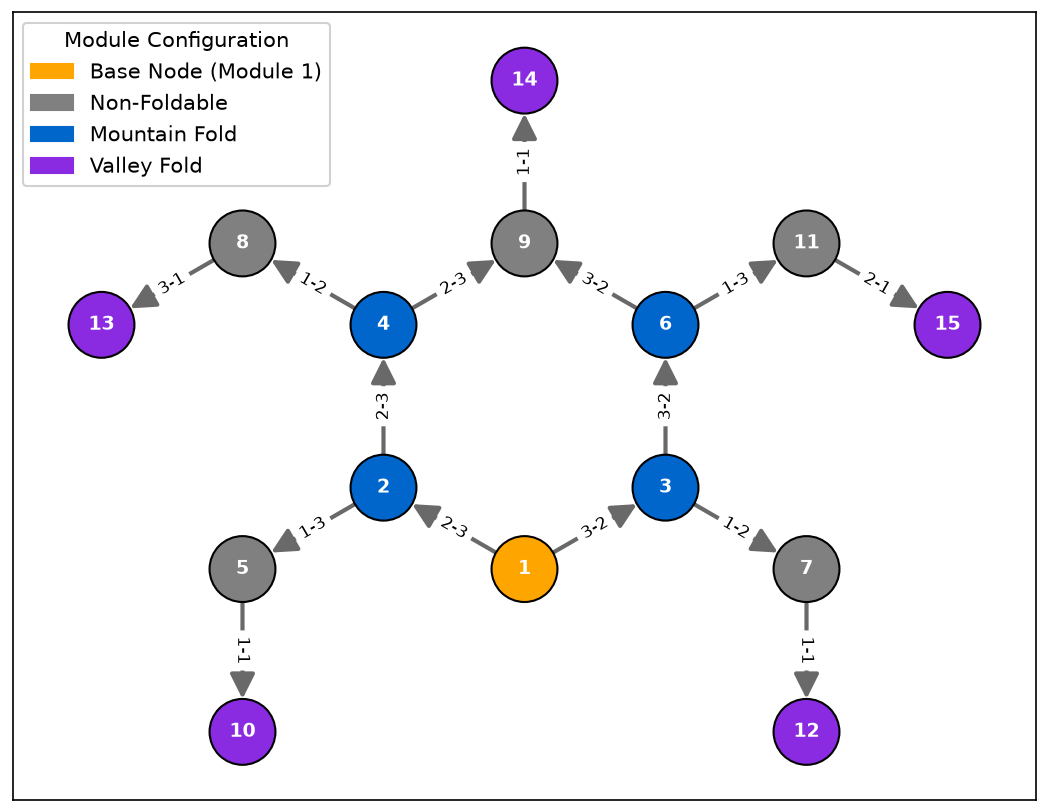
\includegraphics[width=0.75\linewidth]{genotype.png}
    \caption{Example half-genotype: nodes are modules (coloured by fold type), edges labelled by connector port pairs. Only this half is evolved; the full morphology is produced by mirroring (Section~\ref{sec:symmetry}).}
    \label{fig:genotype}
\end{figure}
\begin{figure}[H]
    \centering
    \begin{subfigure}[b]{0.47\linewidth}
        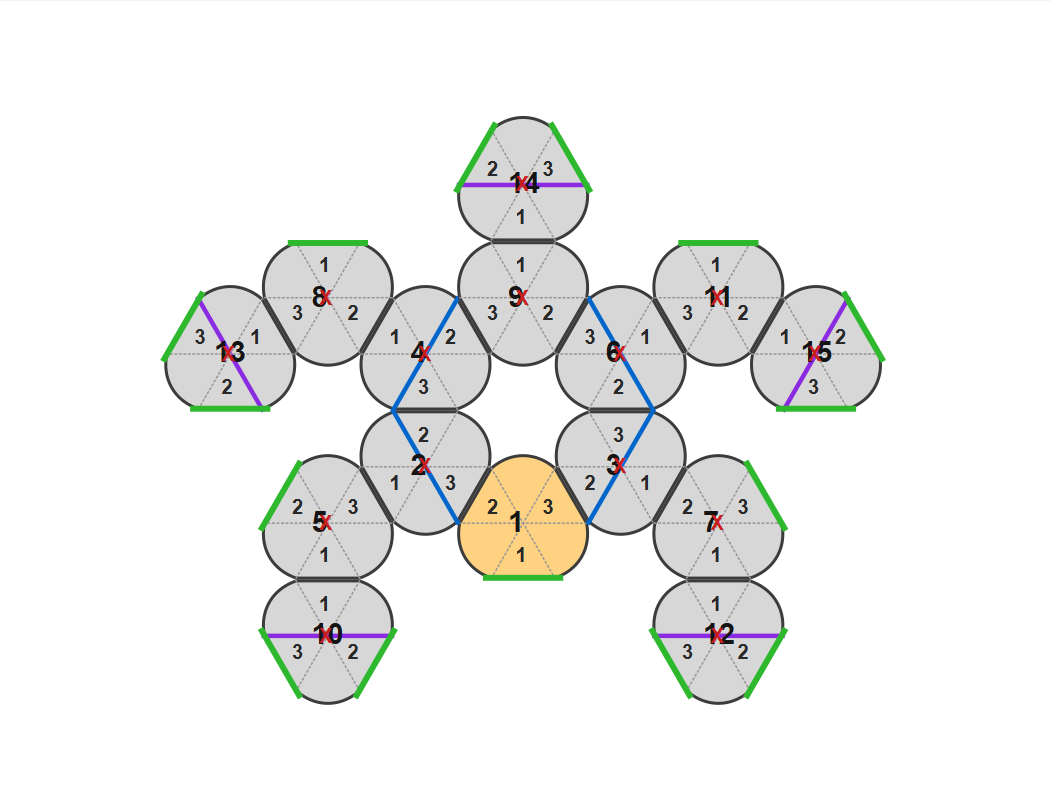
\includegraphics[width=\linewidth]{phenotype.png}
        \caption{2D Phenotype}
        \label{fig:morph-planar}
    \end{subfigure}
    \hfill
    \begin{subfigure}[b]{0.47\linewidth}
        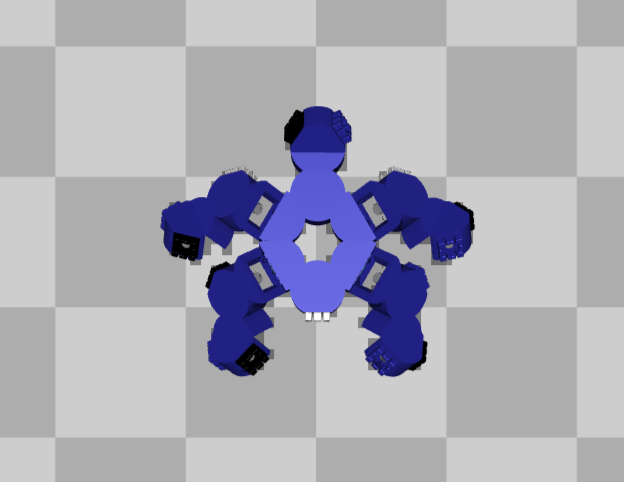
\includegraphics[width=\linewidth]{3d_view_zoomed.png}
        \caption{3D folded phenotype}
        \label{fig:morph-3d}
    \end{subfigure}
    \caption{Example morphologies: (a) 2D planar layout, (b) folded 3D configuration after self-folding.}
    \label{fig:morphologies_example}
\end{figure}

\subsubsection{Bilateral Symmetry and Mirror Construction}
\label{sec:symmetry}
Only one half of the morphology is evolved directly. The root module and its spine child provide the mirror anchors, while the expandable side is connected through the remaining port. During construction, the other side is generated deterministically by reflecting the evolved half. This keeps the final robot bilaterally symmetric and reduces the number of graph decisions required by the search.

The mirror is applied at build time rather than treated as a separate learned action. As a result, every mutation and crossover operates on the same half-graph representation, while the simulator receives the complete structure. The representation reduces redundant solutions without removing the structural edits available to the evolutionary operators.

\begin{figure}[H]
    \centering
    \begin{subfigure}[b]{0.47\linewidth}
        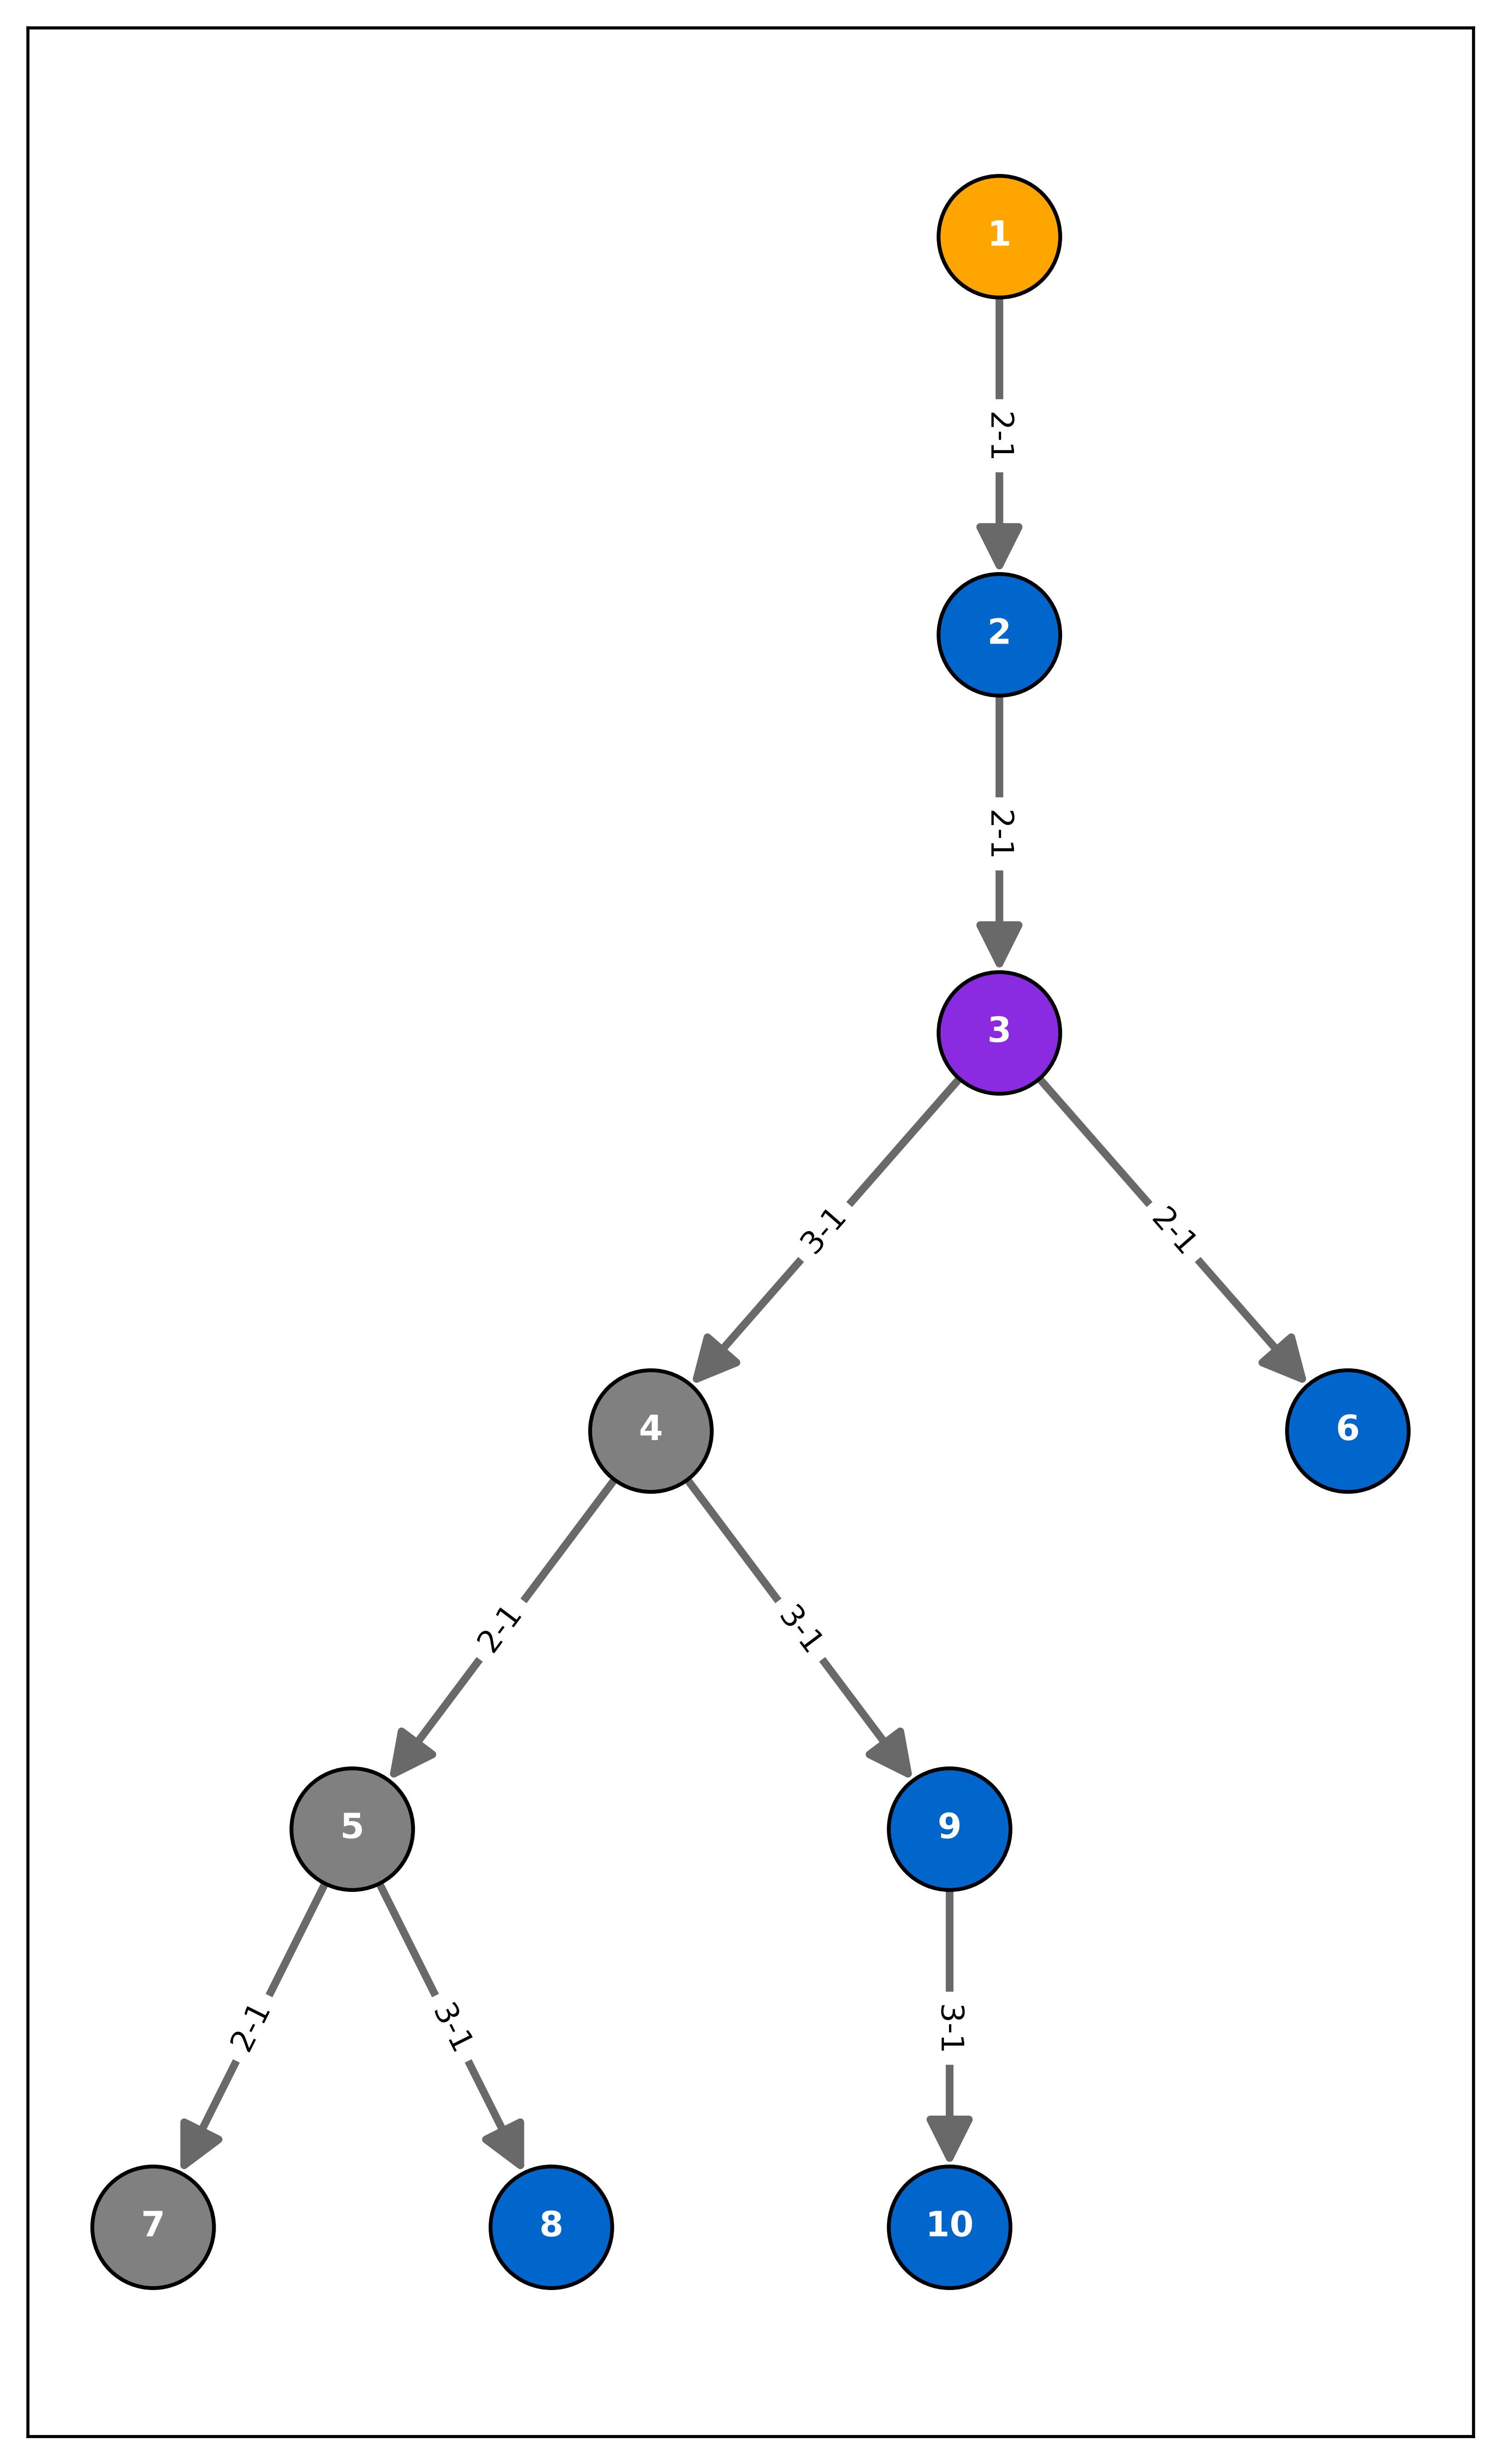
\includegraphics[width=\linewidth]{mirror_graph_before.png}
        \caption{Graph representation of the half-genotype}
        \label{fig:mirror-graph}
    \end{subfigure}
    \hfill
    \begin{subfigure}[b]{0.47\linewidth}
        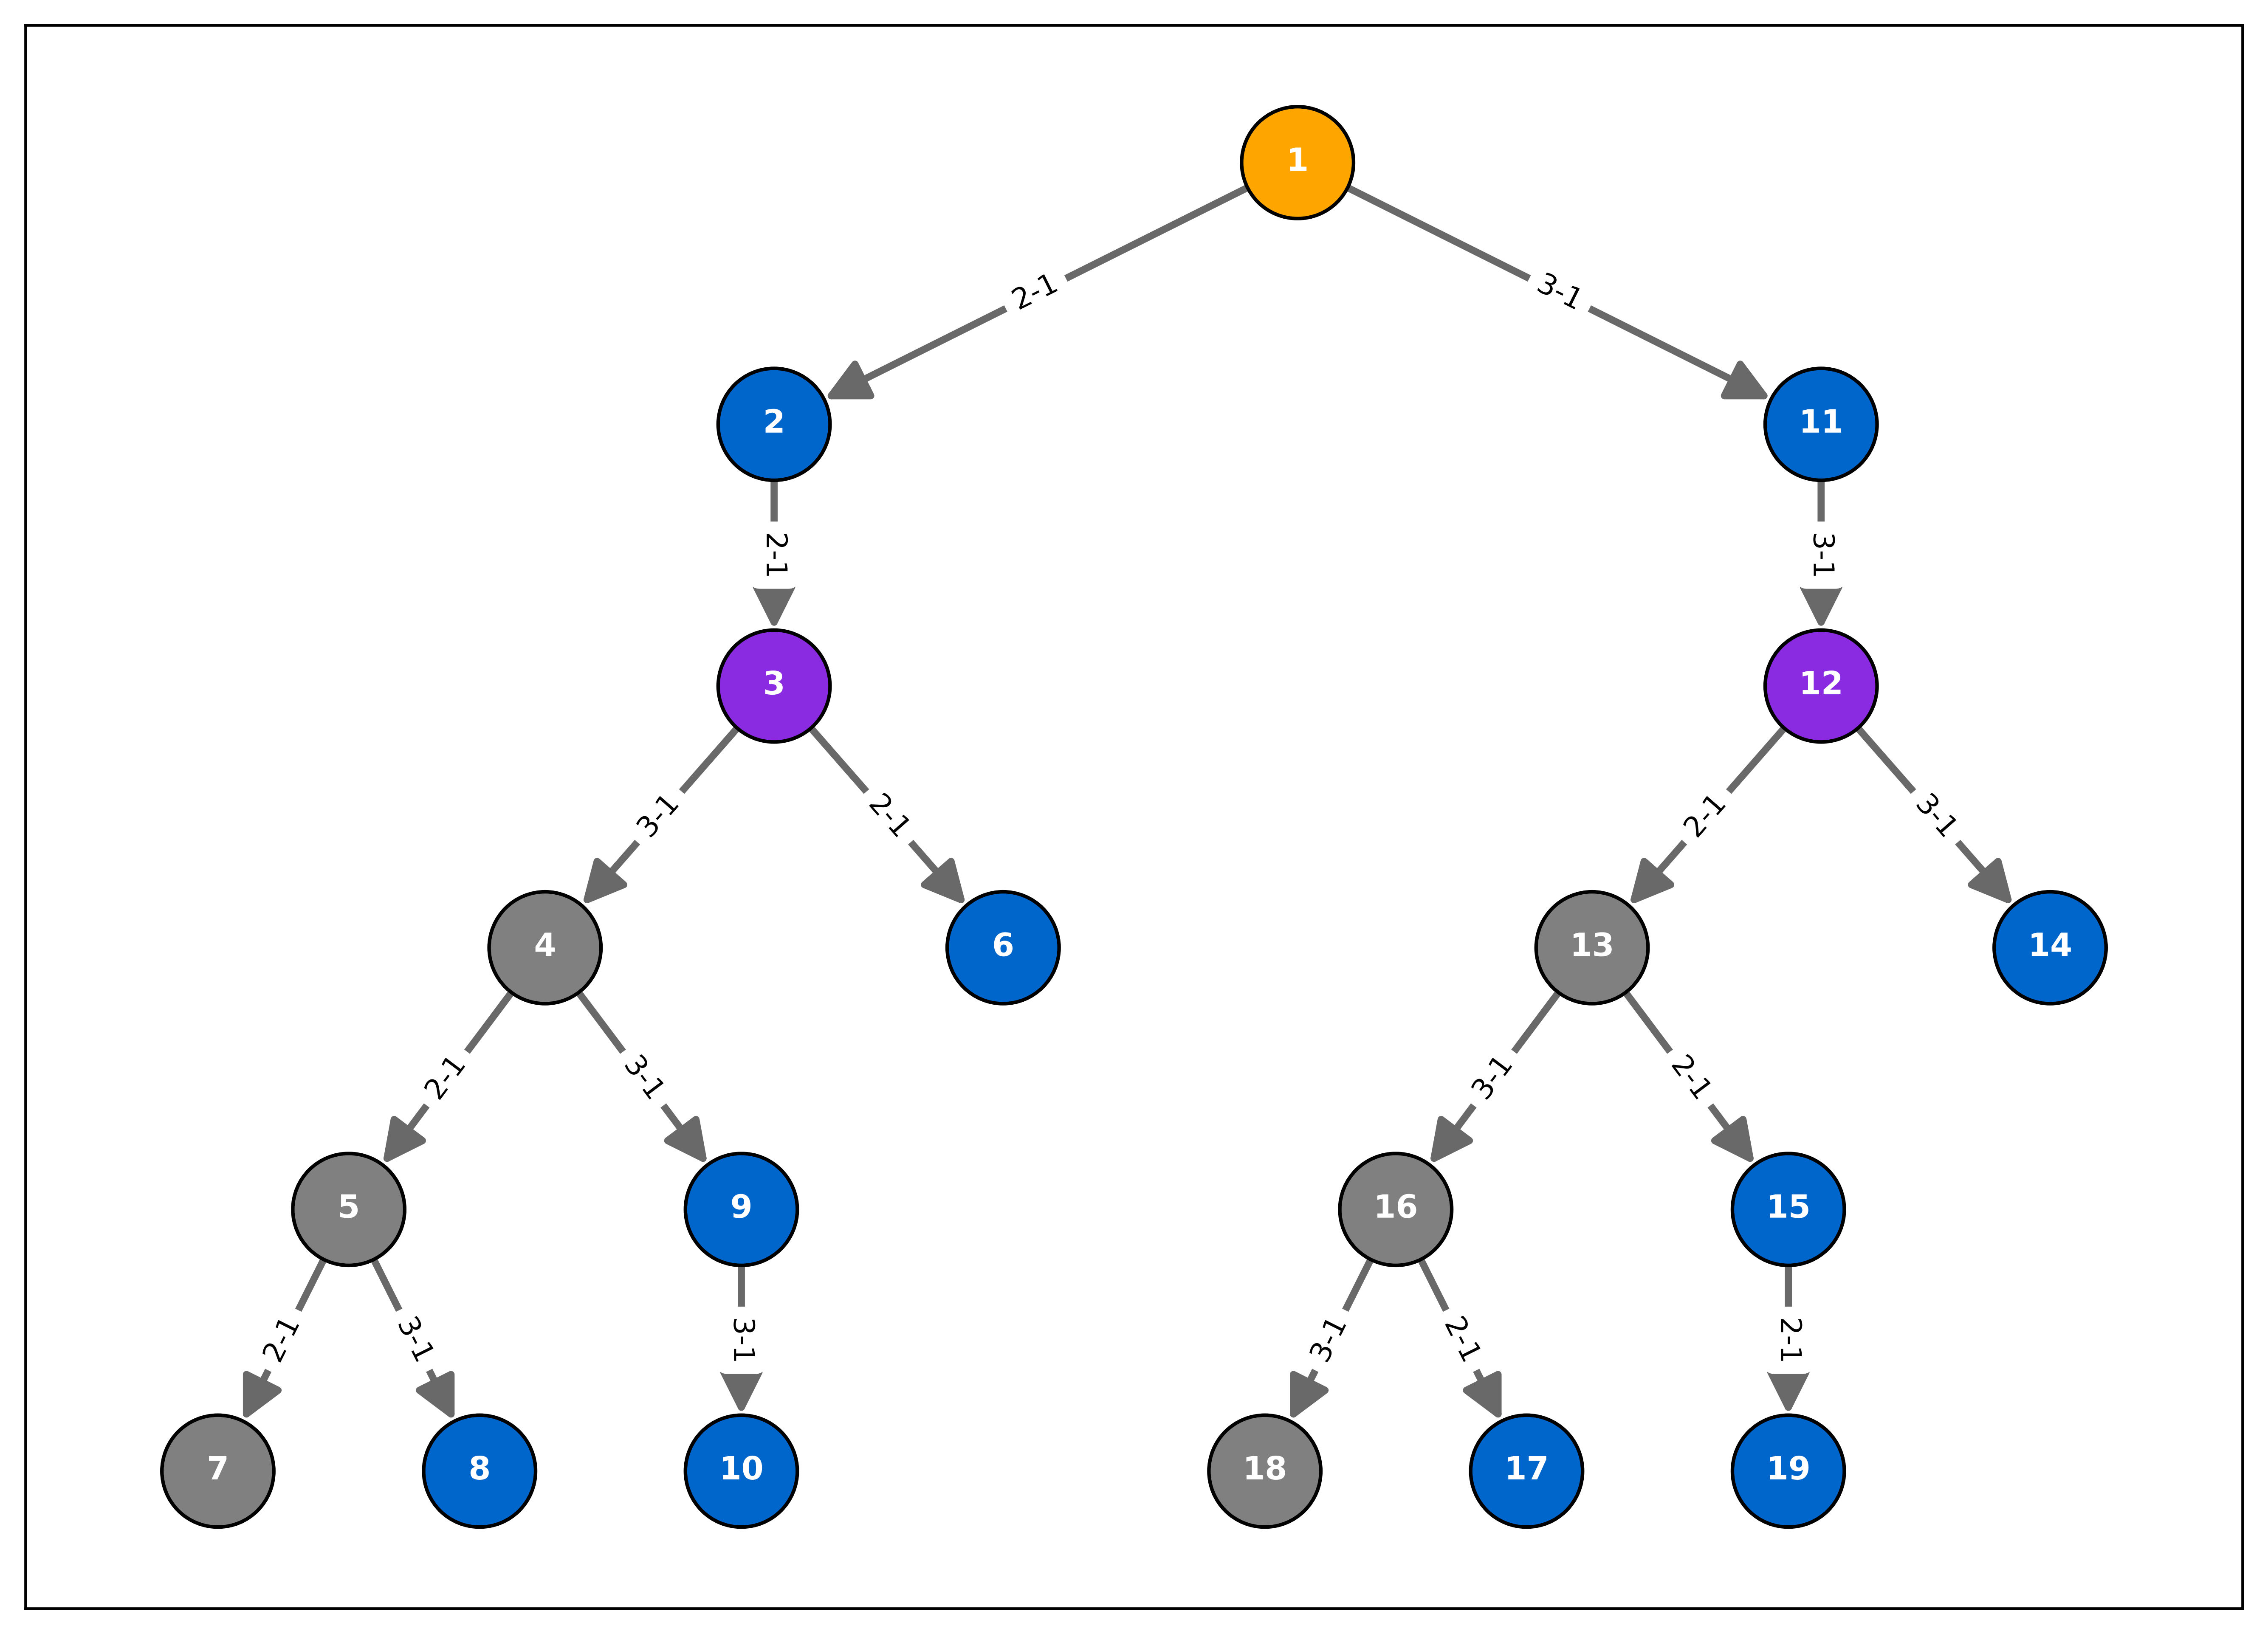
\includegraphics[width=\linewidth]{mirror_graph_after.png}
        \caption{Graph representation of the full genotype after mirroring}
        \label{fig:mirror-graph-after}
    \end{subfigure}
    \caption{Mirror construction: (a) evolved half-genotype, (b) full genotype after deterministic mirroring about the root's spine.}
    \label{fig:mirror-example}
\end{figure}

\subsubsection{Grammar-Legal Mutation and Crossover Operators}
The operator set contains eight mutations and two crossovers: add node, delete node, prune subtree, change fold type, change hinge angle, reconnect a port, toggle a light sensor, change the light hinge angle, graft a subtree and swap subtrees. Each action is masked according to the current graph. Addition requires a free port and the module limit, deletion protects the root and targets a removable leaf, and reconnection must leave valid port assignments.

Invalid action masking was applied to constrain the policy distribution to legal actions at each decision step, as masking has theoretical justification in policy-gradient methods and becomes increasingly important as the fraction of invalid actions grows \citep{huang2020closer}. Grammar masking was therefore selected instead of generating an illegal graph and rejecting it afterwards. Reject-and-retry wastes simulation and policy samples, while a soft penalty asks the policy to learn rules that can be enforced directly. Masking guarantees that sampled structural edits are legal and leaves simulation failure to represent physical or numerical problems rather than simple grammar errors.

Three of the mutation actions are illustrated in Figure~\ref{fig:mutations}.
\begin{figure}[H]
    \centering
    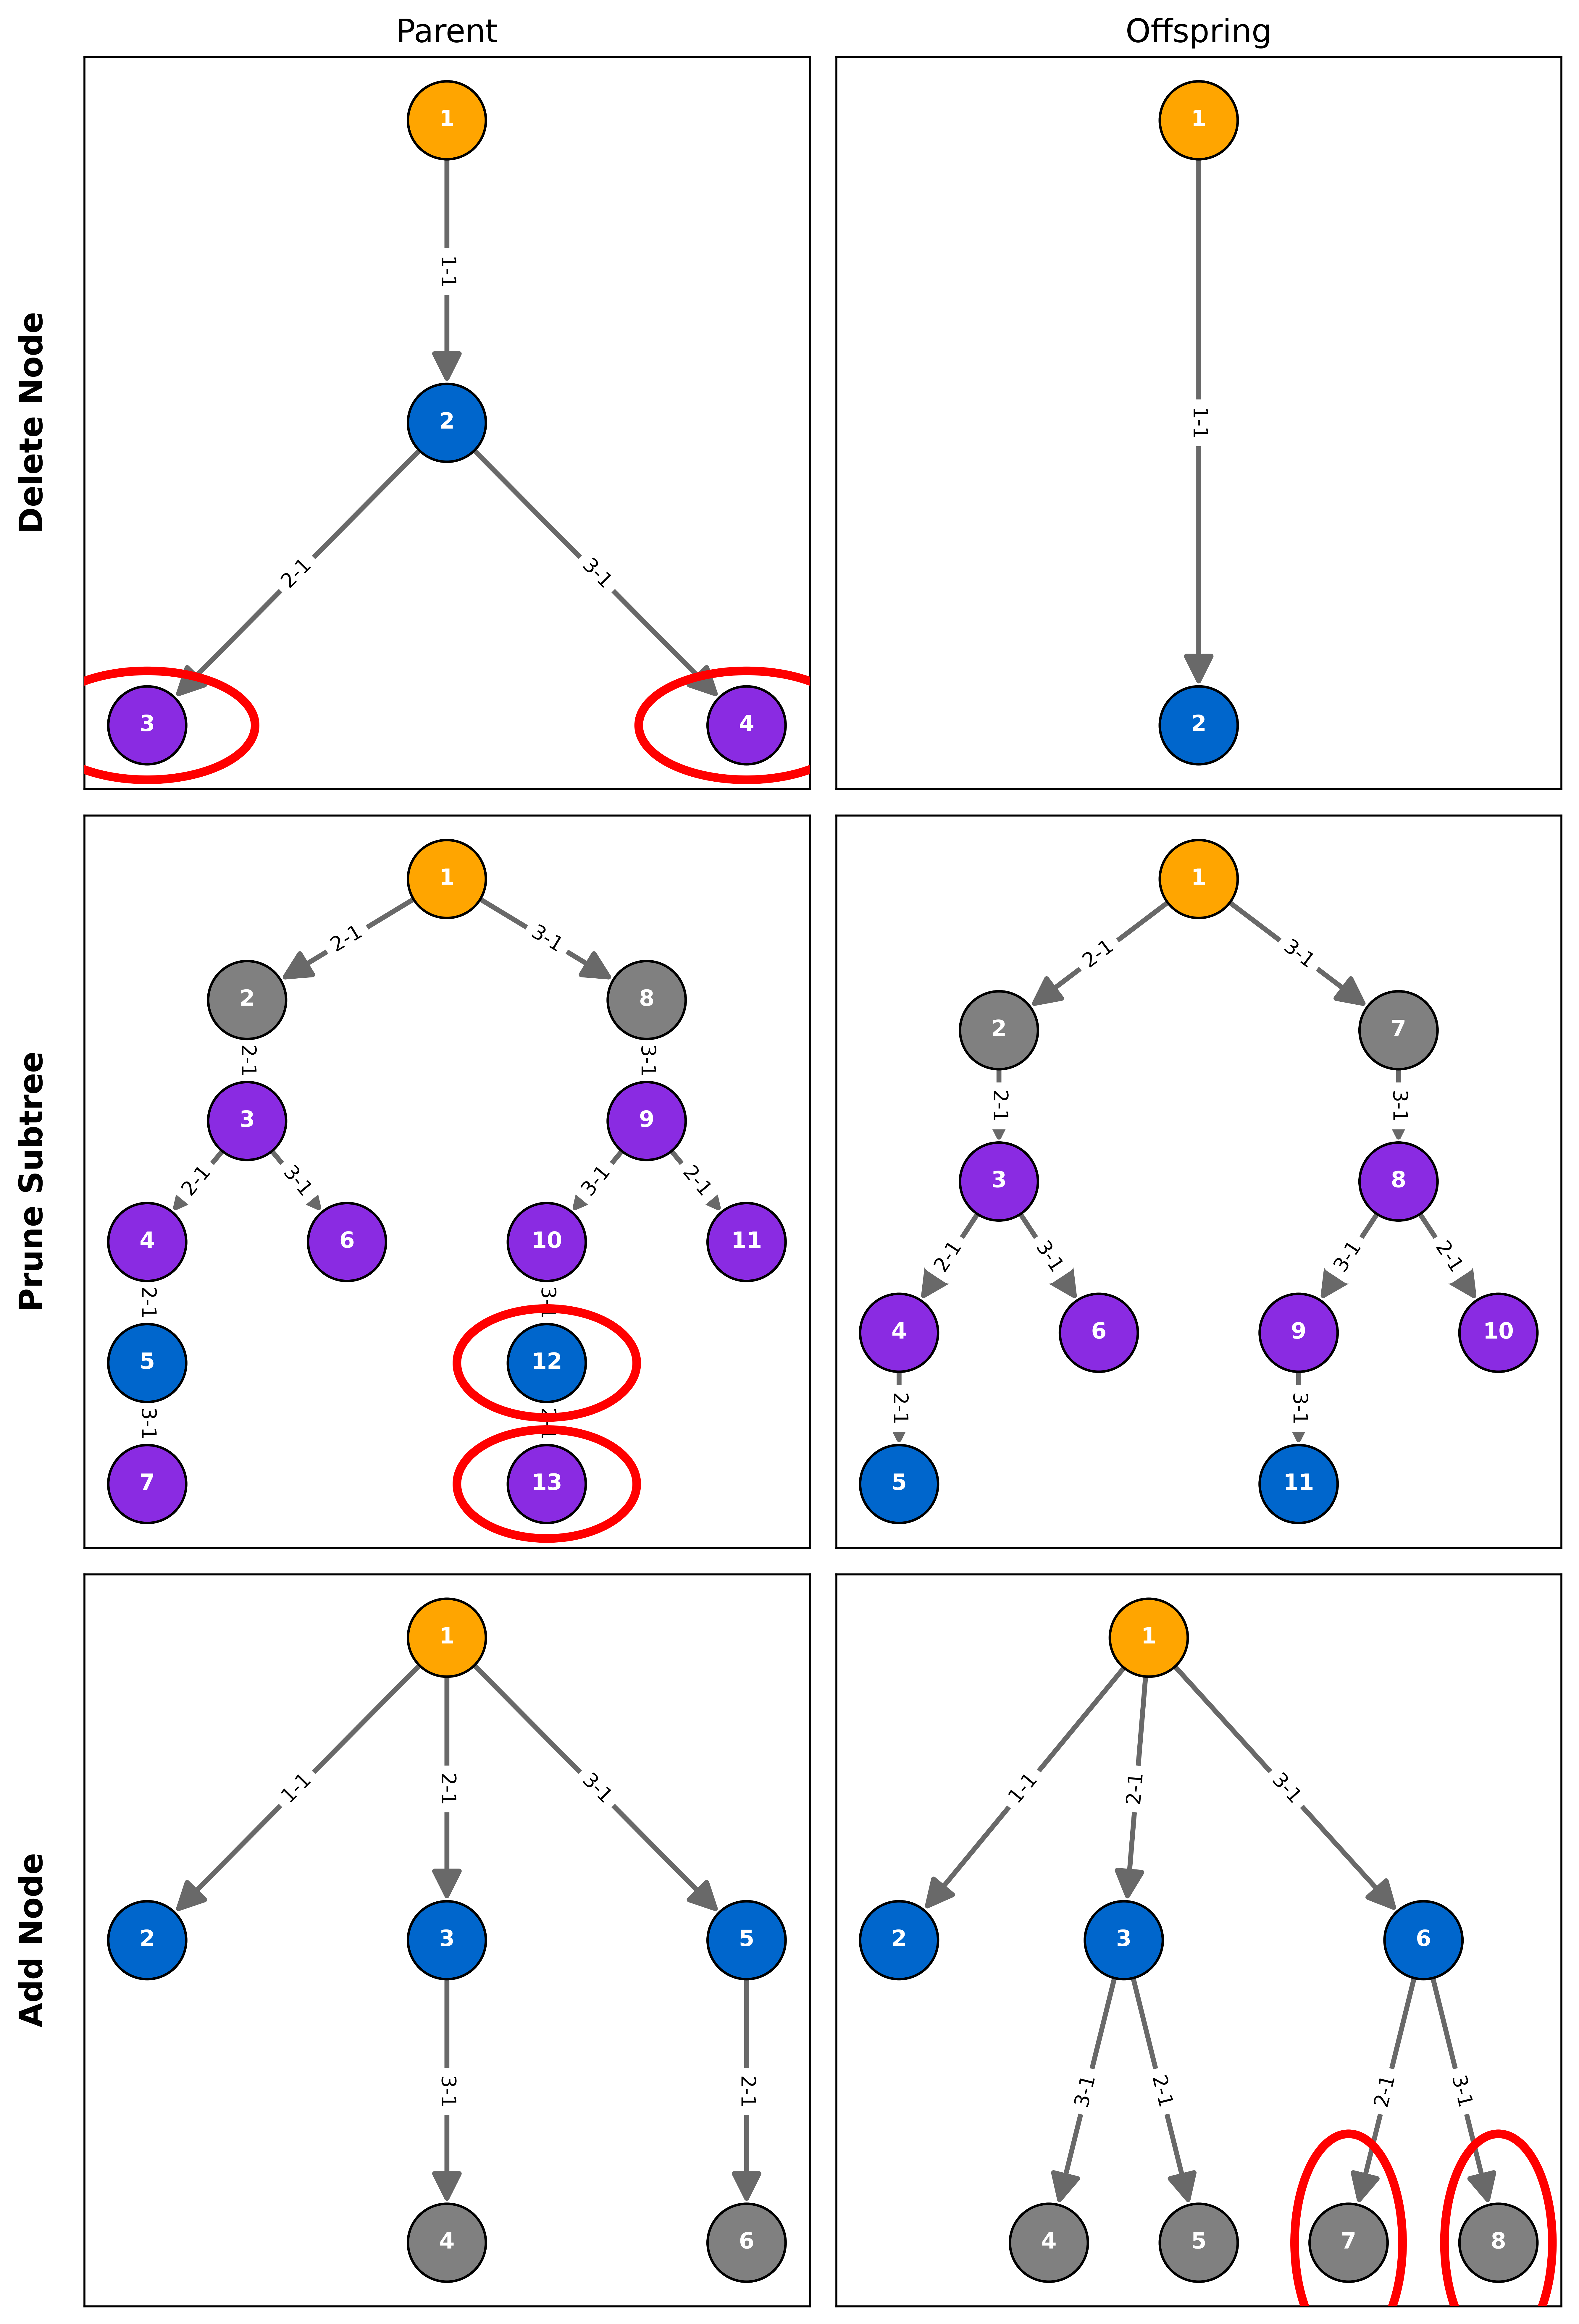
\includegraphics[width=0.65\linewidth]{mutations.png}
    \caption{Three grammar-legal mutation actions, each a real parent$\rightarrow$offspring pair sampled from an evolutionary run (mutated node(s) circled in red): Delete Node, Prune Subtree, Add Node.}
    \label{fig:mutations}
\end{figure}

\subsection{Multi-Objective Fitness Formulation}
\label{sec:objectives}
\begin{equation}
\mathbf{f}=
\left[
\underbrace{v_b}_{f_1},\;
\underbrace{\tilde{H}_{3D}-\tilde{H}_{2D}}_{f_2},\;
\underbrace{\Delta\psi_L-\Delta\psi_b}_{f_3},\;
\underbrace{\frac{v_F-v_b}{v_b}}_{f_4}
\right]
\label{eq:objectives}
\end{equation}
Here, $v_b$ is the baseline folded-gait velocity, $\tilde H_{2D}$ and $\tilde H_{3D}$ are the normalised shape entropies before and after folding, $\Delta\psi_b$ and $\Delta\psi_L$ are the baseline and left-stimulus yaw changes, and $v_F$ is the velocity under the front stimulus. The four components are maximised in the attractive run. In the repulsive run, the signs of the two light-response preferences are reversed by the objective configuration rather than by changing the measured signed quantities.
The objective vector is evaluated after folding and actuation. The first component measures folded-gait velocity. The second measures the change in normalised shape entropy between the flat and folded forms. The final two components measure changes in yaw and speed under light stimulation relative to their baselines. All four objectives are maximised in the attractive run; the optimisation direction of the two light-response objectives is changed in the repulsive run.

\subsubsection{Folded-Gait Locomotion and Shape-Entropy Objectives}
Velocity is measured after the torque ramp so that the initial settling period does not dominate the result.

Shape entropy measures the structural complexity of a morphology from its occupancy pattern. The shape is voxelised, and for each odd window size $W$, the local occupancy pattern around every occupied cell is recorded. The Shannon entropy of the resulting pattern-frequency distribution is
\begin{equation}
H(W) = -\sum_{i=1}^{N_W} p_i(W)\log_2 p_i(W),
\label{eq:shape-entropy}
\end{equation}
where $p_i(W)$ is the probability of pattern $i$ at window size $W$ and $N_W$ is the number of distinct patterns observed. $H(W)$ is normalised by $\log_2 N_W$ so that different window sizes are comparable, and the normalised values are averaged across window sizes to give one scalar per shape. This connects to prior work on shape entropy in self-assembly \citep{van2014understanding, van2014entropically} and persistent/morphological entropy in topology and geometry \citep{atienza2019persistent, liu2024morphological}. Applying this to the flat and folded occupancy grids gives $\tilde H_{2D}$ and $\tilde H_{3D}$ respectively. The reported folding-complexity objective is $f_2=\tilde H_{3D}-\tilde H_{2D}$, so a positive value indicates greater measured structural complexity after folding. The raw two-dimensional and three-dimensional entropy values are retained for the later relationship analysis.

\subsubsection{Pheromone Reaction-Primitive Tests}
\label{sec:pheromone-tests}
Each light-response objective uses two stages. The first stage measures the baseline behaviour without the relevant light stimulus. The second stage applies either a left-side stimulus for yaw or a front stimulus for speed and measures the changed response. The yaw objective is the difference between the light and baseline rotations, while the speed objective is the relative change from baseline speed.

A separate baseline stage is important because the robot can naturally curve or drift during its magnetic gait. The comparison must therefore use a travel-aligned local frame established for that objective, rather than the trajectory produced during the stimulated rollout. The settled pose is also not physically rotated simply to define the frame. This keeps the measured difference attributable to the light condition as far as the simulation permits and avoids confusing pre-existing gait direction with reaction behaviour.

The light stimulus itself is a floor-level rectangular light patch (referred to here as the luminance sheet) that a MuJoCo \texttt{<light>} is repositioned and resized to cover for a given test stage; a light-sensitive joint reacts once the illuminance measured at its on-body sensor site exceeds a fixed lux threshold. Rather than snapping instantly to its evolved target angle when triggered, each light-sensitive hinge eases toward that target through a first-order exponential relaxation
\begin{equation}
\theta(t) = \theta_{\text{set}} + \left(\theta_{\text{prev}} - \theta_{\text{set}}\right)e^{-\Delta t/\tau_c},
\label{eq:light-joint-lag}
\end{equation}
recomputed once per physics step, where $\theta_{\text{set}}$ is the joint's evolved light-detection hinge angle while the sensor is lit and its baseline (non-light) gait angle once the sensor is no longer lit, $\Delta t$ is the elapsed simulation time since the previous step, and $\tau_c$ is a fixed time constant (1\,s). The same formula and time constant govern both the onset and the release of the response, so the joint eases smoothly toward the light-triggered angle and smoothly back to baseline rather than snapping between the two.

\begin{figure}[H]
    \centering
    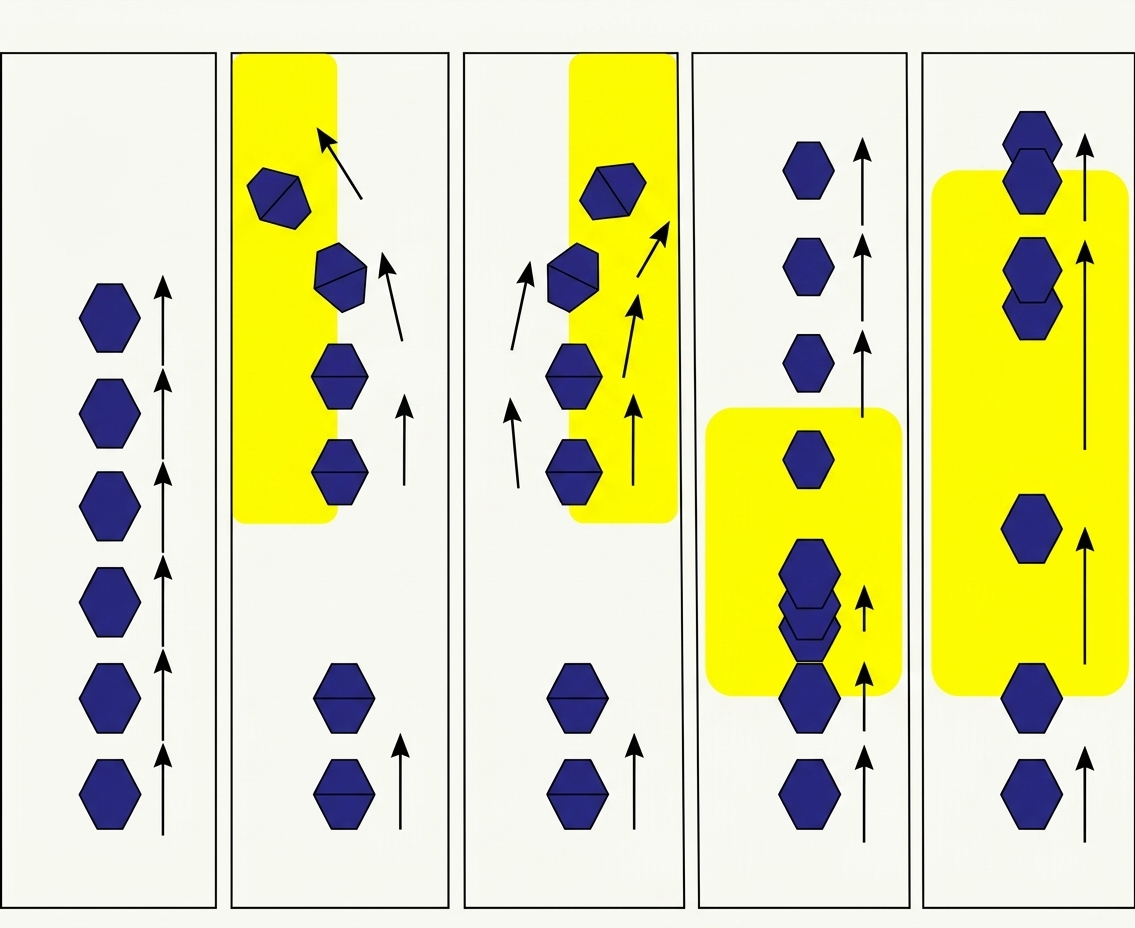
\includegraphics[width=0.85\linewidth]{primitives.png}
    \caption{Five pheromone-detection primitives: (a) baseline, (b)/(c) left/right-stimulus yaw response, (d)/(e) front-stimulus speed response against slower/faster baselines.}
    \label{fig:primitives}
\end{figure}

\begin{figure}[H]
    \centering
    \begin{subfigure}[b]{0.47\linewidth}
        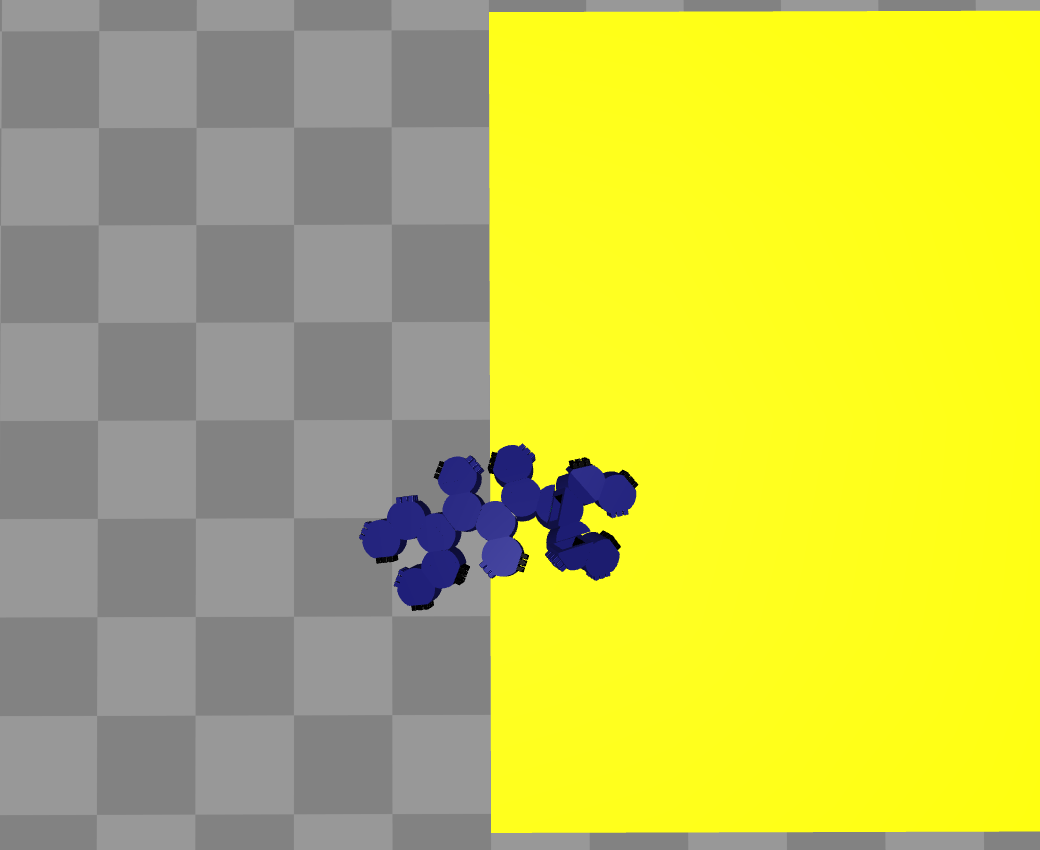
\includegraphics[width=\linewidth]{left_light_stage.png}
        \caption{Left-stimulus stage (yaw response)}
        \label{fig:light-stage-left}
    \end{subfigure}
    \hfill
    \begin{subfigure}[b]{0.47\linewidth}
        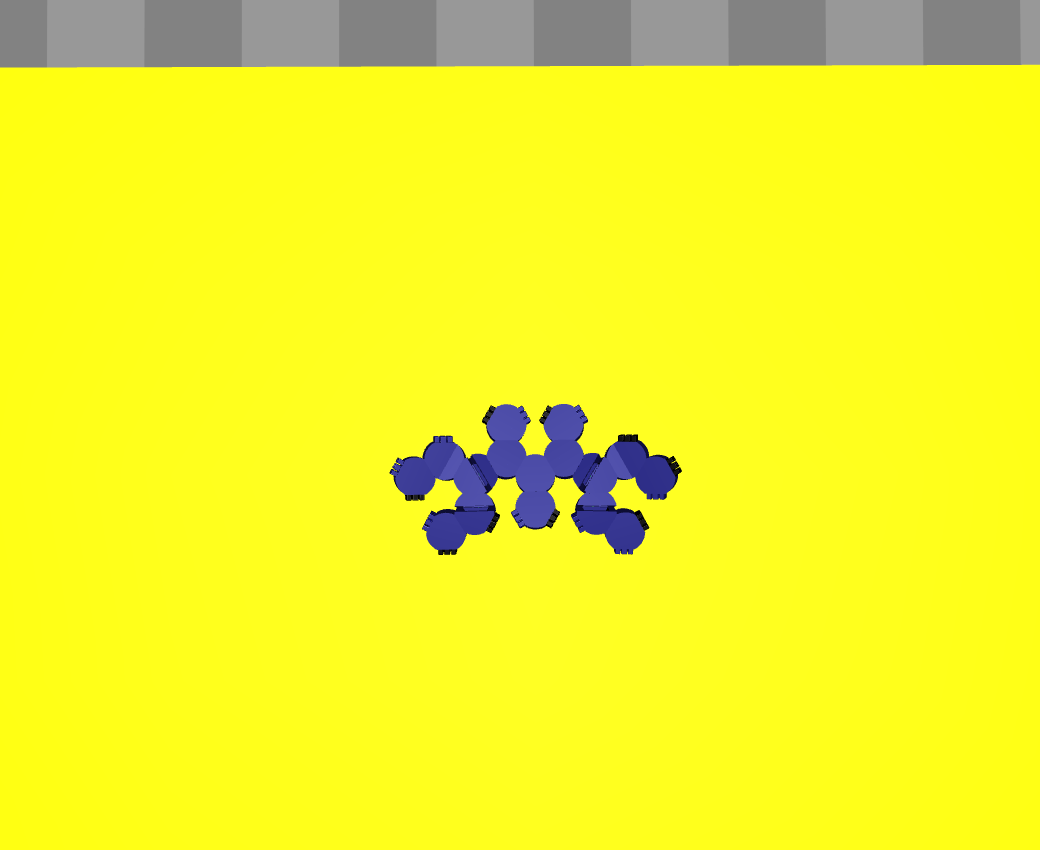
\includegraphics[width=\linewidth]{front_light_stage.png}
        \caption{Front-stimulus stage (speed response)}
        \label{fig:light-stage-front}
    \end{subfigure}
    \caption{MuJoCo setup for the two pheromone reaction-primitive tests (yellow = luminance sheet); "left"/"front" are relative to the robot's travel-aligned frame (Section~\ref{sec:pheromone-tests}), not the camera view.}
    \label{fig:light-stages}
\end{figure}



\subsubsection{Attractive versus Repulsive Response Configuration}
Attractive and repulsive behaviour were implemented as separate evolutionary runs. Both runs use the same signed measurements: positive yaw denotes turning towards the light and positive speed response denotes speeding up. The optimisation direction is then changed for the repulsive run so that turning away and slowing down are preferred. A single run containing both directions would ask the same light-hinge variable to increase and decrease at once, creating a self-contradictory objective pair. Separate runs make the intended behaviour explicit and allow their morphologies to be compared directly.

\subsection{RL-Guided Actor-Critic for Structural Edits}
\label{sec:rl-actor-critic}
The structural-edit policy receives an ordered pair of parent half-genotypes. Each graph is represented by nine node features: module type, normalised hinge angle, depth, free-port fraction, root status, light sensitivity and light-hinge angle. An attention-based Graph Transformer encoder was used to embed the variable-size genotype graphs, because graph multi-head attention performs message passing over edges while incorporating edge features into the propagation mechanism \citep{shi2020masked}. The encoder produces representations for the variable-size graphs using hidden dimension 32, two Transformer blocks and four attention heads. Separate actor and critic networks use this graph representation and a global mean readout.

The action is sampled hierarchically. First, the actor selects one of eight mutation actions or two crossover actions. It then selects legal target nodes, ports and parameters. The mask is applied at each stage, so the policy cannot select a root deletion, an unavailable port or an action that exceeds the module limit. The reward is the change in scalarised four-objective fitness from parent to child; collision and instability outcomes are excluded from the reward entirely rather than penalised (below). PPO was used to update the structural-edit policy because it alternates data collection with optimisation of a clipped surrogate objective, supports multiple epochs of minibatch updates per batch, and offers a favourable balance between simplicity and sample efficiency \citep{schulman2017proximal}; it is updated once per generation using the offspring decisions as one-step transitions.

This policy guides variation, not locomotion control. The policy chooses how the graph is changed, while MuJoCo supplies the physical evaluation.

The architecture described above is the final design used to produce the results in Chapter~\ref{ch:results}, and differs from an earlier version in three respects motivated by training diagnostics (the reasoning behind each change, and the evidence that prompted it, is presented as Results in Section~\ref{sec:rl-diagnostics} rather than repeated here, since it is evidence, not method):

\begin{itemize}
    \item \textbf{Shared encoder architecture:} The actor and critic share a single Graph Transformer encoder rather than each training an independent copy, so that both losses contribute gradient signal to the same graph representation instead of each network having to learn one from a much smaller effective sample.
    \item \textbf{Entropy decay schedule:} The entropy coefficient decays across training rather than remaining fixed, keeping exploration pressure higher earlier in a run when a structural action's probability is most at risk of collapsing on limited evidence.
    \item \textbf{Collision and instability outcomes excluded from the reward stream:} An earlier version recorded a fixed penalty whenever a proposed child collided or failed simulation, giving the policy a direct learning signal against those outcomes. This was removed rather than rescaled: any reward mechanism that lets the policy compare outcomes across action types can exploit the fact that every structural action (Add Node, Graft Subtree, and so on) carries some baseline collision risk simply by changing the graph, while several non-structural actions (e.g.\ Toggle Light Sensor) structurally cannot trigger the collision gate at all. In practice this caused the policy to collapse onto whichever action type could never be penalised, regardless of how the penalty was scaled (Fig.~\ref{fig:rl-cp-action-distribution}). Collision and instability outcomes are now excluded from the reward stream entirely -- neither the collision gate's own rejections nor a post-simulation instability flag are ever recorded as a reward -- so the reward the policy sees always reflects genuine scalarised design-quality change, never a collision or instability outcome. Both arms still pay the same wasted-retry cost when a proposed child fails the collision gate; only the RL arm's reward signal is affected.
\end{itemize}

\begin{figure}[H]
    \centering
    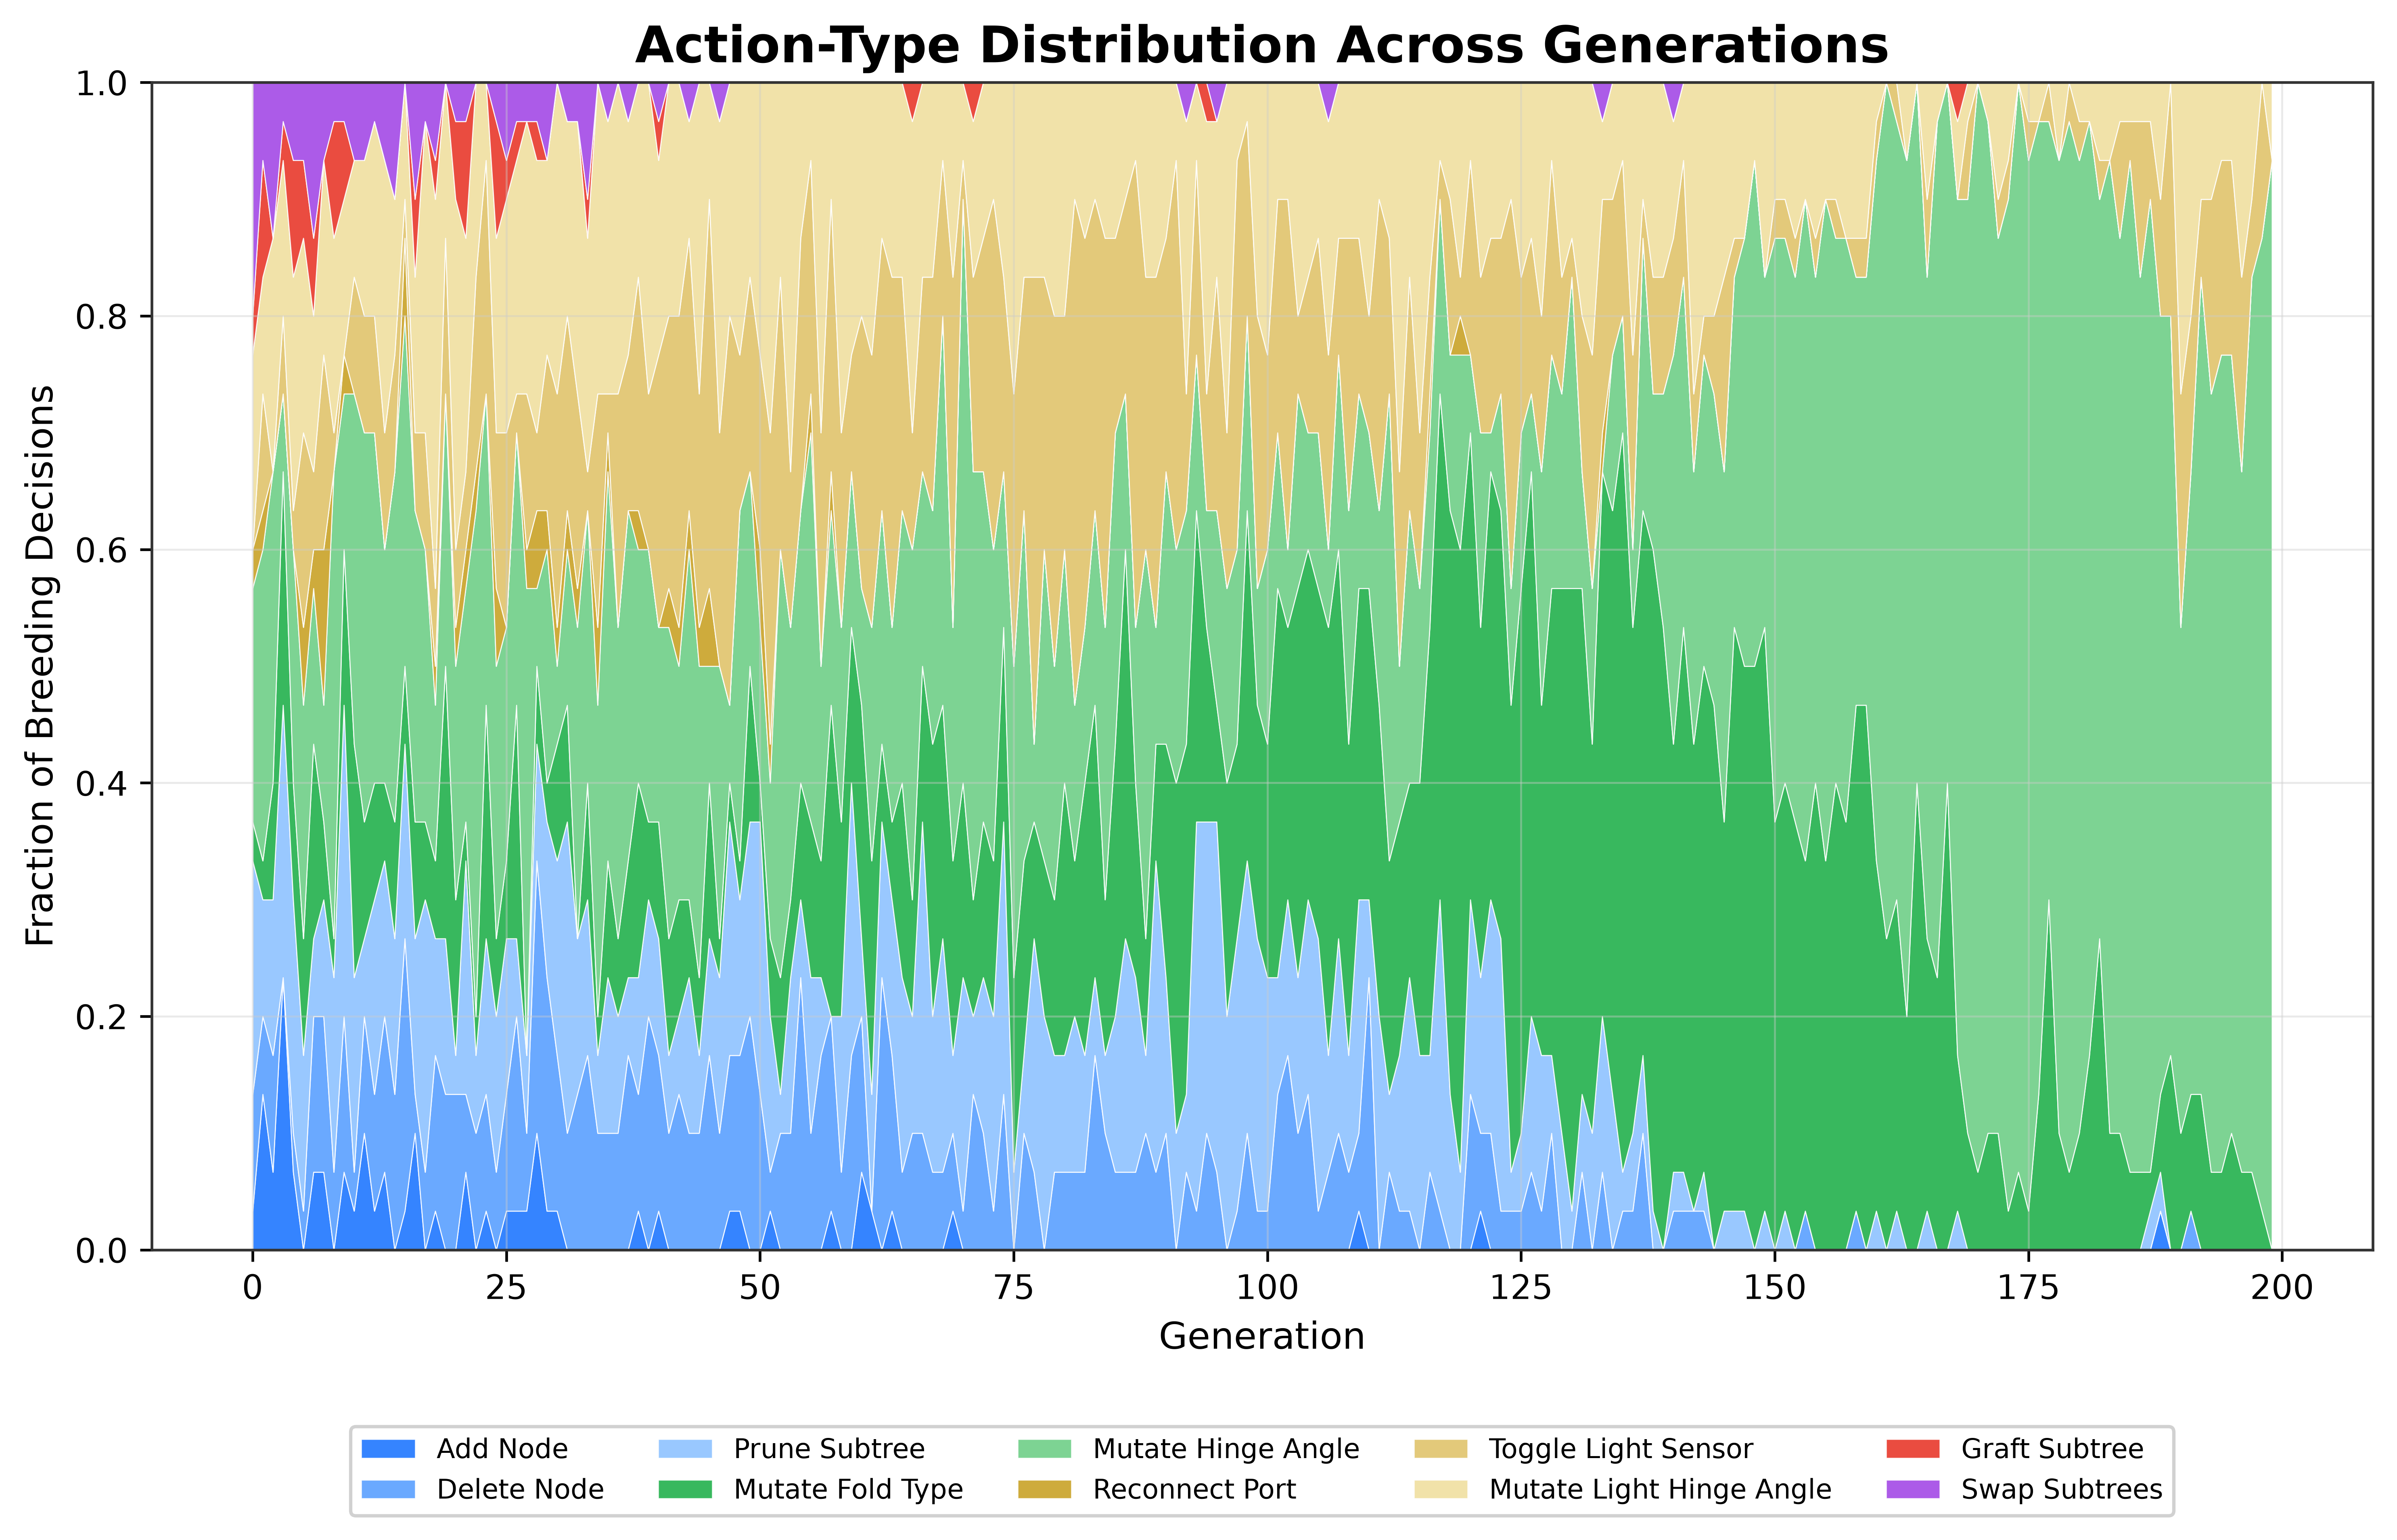
\includegraphics[width=0.85\linewidth]{rl_cp_action_distribution.png}
    \caption{Breeding-decision action distribution per generation for the earlier flat-penalty reward design. By generation 150--200 almost every decision is Mutate Hinge Angle or Mutate Fold Type -- the collapse that motivated removing collision outcomes from the reward stream entirely.}
    \label{fig:rl-cp-action-distribution}
\end{figure}

The objective-normalisation range used by the scalarised reward (Eq.~\ref{eq:reward-appendix}'s $f_n^{-}, f_n^{+}$) starts empty and is updated by every individual's objective values as they are scored, beginning with the first individuals evaluated from the initial Sobol-sampled population; there is no separate warm-start step that pre-computes a range before the first policy update. The same online min/max update rule is used throughout the run, so the range simply reflects the fullest set of objective values observed so far at any given point.

These changes -- particularly excluding collision and instability outcomes from the reward stream -- prevent the reward signal for one action type from being computed relative to a shared, cross-action-type baseline that a handful of risky outcomes can dominate. They do not, on their own, guarantee that every action type's reward estimate is equally reliable: action types sampled less often (Section~\ref{sec:rl-diagnostics} reports the exact counts) still have noisier reward and advantage estimates than the more common mutation actions simply from having fewer observations, which is discussed as a remaining limitation in Section~\ref{sec:rl-diagnostics} rather than a solved problem.

\subsection{NSGA-III Environmental Selection}
NSGA-III was used for environmental selection because it was designed for many-objective optimisation with four or more objectives and preserves diversity through reference-point-based nondominated sorting \citep{deb2014evolutionary}. It ranks individuals using the complete four-objective vector rather than the scalarised value used for the PPO reward. All objectives are converted to a minimisation form for pymoo, while the attractive or repulsive configuration determines the direction of the two light-response objectives. Reference directions are used to retain solutions across the objective space. This is appropriate for four objectives because a single best score would hide useful trade-offs, while reference-direction niching helps maintain spread.

The number of reference directions is derived from the population size rather than fixed, so that niching resolution scales when the population is enlarged; a fixed reference-direction count tuned for a small population would otherwise under-provision diversity preservation once the population grows, since each direction would then have to represent proportionally more individuals. Selection also carries elitism: the best individuals found so far are retained explicitly across generations rather than being at risk of loss purely through the stochastic breeding and evaluation process, so that a strong candidate is not accidentally dropped from the population before its trade-offs have been fully explored by variation.

Feasibility is handled before objective comparison. Structural validity is enforced during graph construction, mirroring and grammar-masked variation, so illegal structural individuals do not need a separate violation score. Simulation failure or instability is treated separately as an infeasible evaluation. Thus, the collision gate handles representation-level feasibility, whereas the simulation constraint records whether a legal structure can also be evaluated successfully.

\subsection{Implementation and Computational Pipeline}
\begin{figure}[H]
    \centering
    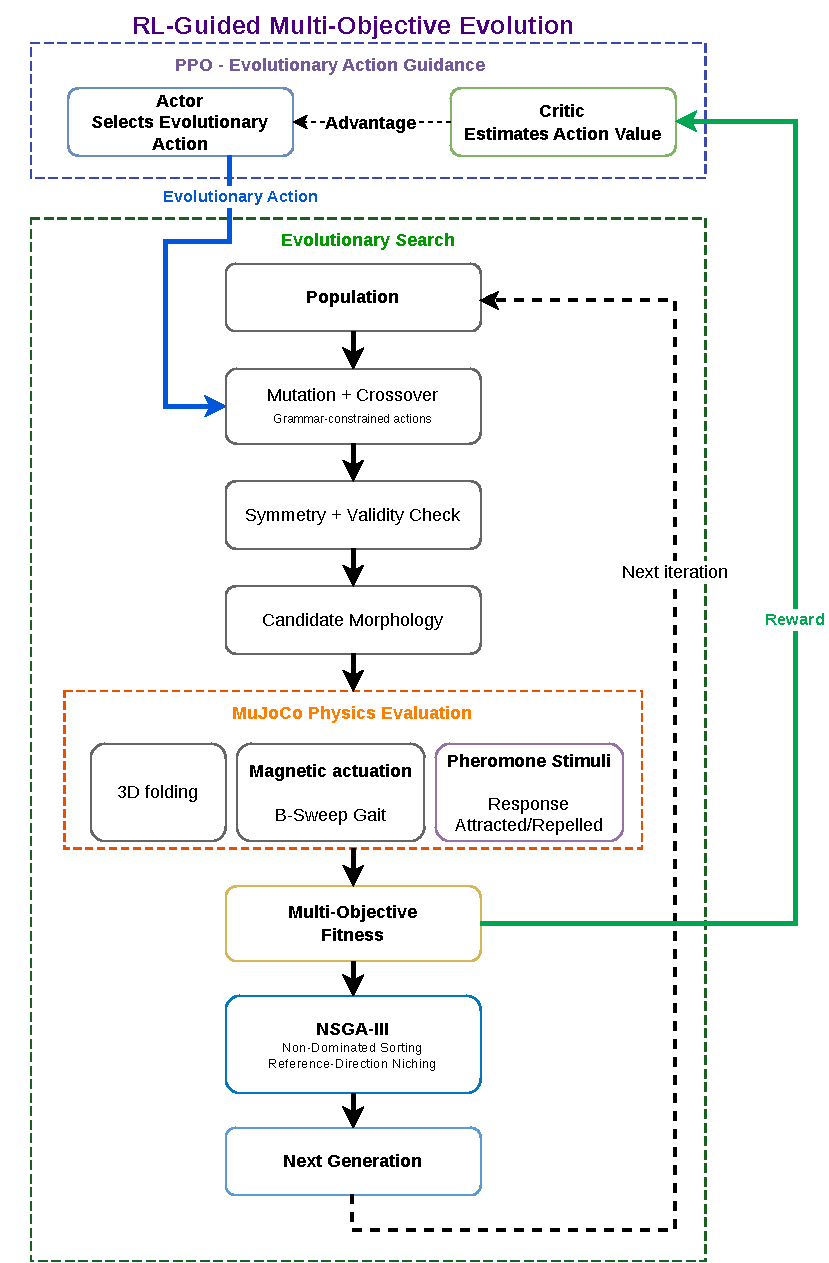
\includegraphics[width=0.85\linewidth]{framework_pipeline.pdf}
    \caption{End-to-end evolutionary pipeline: PPO-selected structural edit $\rightarrow$ mirroring and collision check $\rightarrow$ MuJoCo evaluation (B-sweep gait and pheromone tests) $\rightarrow$ PPO reward and NSGA-III selection for the next generation.}
    \label{fig:pipeline}
\end{figure}
The implementation evaluates individuals in parallel operating-system processes. For each generation, graph data are converted to MJCF files, checked and passed to MuJoCo workers. Results are stored with the individual and are used by both the PPO update and NSGA-III selection. Checkpoints contain the generation, population, random-number state, training state and objective-normalisation information, allowing a run to resume without restarting from the initial population.

An evaluation cache hashes deterministic graph evaluations and avoids simulating unchanged individuals again, including carried-over survivors. The project summary reports approximately 2 minutes per generation with parallel evaluation in computer with 6 Physical cores.

\subsection{Simulation and Training Configuration}
The main reported runs (Chapter~\ref{ch:results}) used a population of 30 individuals over 300 generations, matching the generation axis of Figs.~\ref{fig:convergence}--\ref{fig:pareto-front}. Each individual gait rollout was configured for seven seconds, but an individual is not evaluated with only one such rollout: the magnetic-field sweep runs it at each of the three candidate field strengths (0.001, 0.008 and 0.025\,T) plus a final re-run at the winning field, and the three light-response stages (Section~\ref{sec:pheromone-tests}) run separately again, for seven (baseline), ten (left-stimulus) and ten (front-stimulus) seconds -- so the total simulated time per individual is well above seven seconds. The fresh-run random seed was 42. Every result reported in this thesis, including the RL-versus-standard-breeding comparison (Section~\ref{sec:rl-vs-random}), comes from a single seed per configuration, so variation between independent runs under the same settings has not been measured; this is discussed as a limitation in Section~\ref{sec:limitations}.

The same simulation and objective definitions were used for attractive and repulsive response runs. A candidate had to pass the graph and collision checks before being evaluated; simulation instability was still recorded as a failed evaluation. The number of generations completed differs between the reported output directories, since \texttt{N\_GENERATIONS} is a module-level configuration constant that was changed between runs rather than a fixed setting; Appendix~\ref{app:reproduce} lists every such configuration constant and where it is set.

\subsection{Baseline Comparison Arm}
The random baseline uses the same genotype, grammar masks, collision gate, simulation, objective calculation and NSGA-III survival procedure as the RL-assisted arm. Its only change is that action types and parameters are selected uniformly rather than by the trained PPO policy. This makes the comparison useful because any difference is more directly associated with learned variation choices, rather than with a different simulator or selection rule.

\subsection{Evaluation Metrics}
\label{sec:eval-metrics}
Hypervolume (HV) is the main many-objective convergence measure because it combines improvement and spread of the non-dominated set. GD, IGD and IGD+ were not used because this engineering problem has no known true Pareto front; constructing a best-known front from the same simulation runs would make the comparison partly circular. Best and mean scalarised fitness are included as a simpler view of population progress, but they are not used as the NSGA-III selection criterion.

The action distribution records how often each structural operator is chosen and can reveal collapse of mutation or crossover actions. Per-action reward and policy-loss plots help investigate why an action becomes common or rare. Finally, collision rate, defined as $n_{\mathrm{collided}}/n_{\mathrm{offspring}}$, indicates how many proposed offspring fail the geometric feasibility check. These metrics together describe optimisation progress and the behaviour of the operator policy.


\chapter{Results}
\label{ch:results}
This chapter reports the outcomes of the framework described in Chapter~\ref{ch:methodology}, presented in the order basic objectives, advanced objectives, then an honest account of the RL-guided search's current limitations. Sections~\ref{sec:convergence-hv} and~\ref{sec:pareto-results} examine evolutionary convergence and Pareto trade-offs; Section~\ref{sec:entropy-velocity} relates morphological complexity to locomotion; Section~\ref{sec:evolved-morphologies} shows evolved morphologies under the attractive and repulsive pheromone configurations; and Sections~\ref{sec:rl-vs-random} and~\ref{sec:rl-diagnostics} compare the RL-assisted search against a random baseline and analyse the RL policy's training behaviour in detail.

\section{Evolutionary Convergence and Hypervolume}
\label{sec:convergence-hv}
\begin{figure}[H]
    \centering
    \begin{subfigure}[b]{\linewidth}
        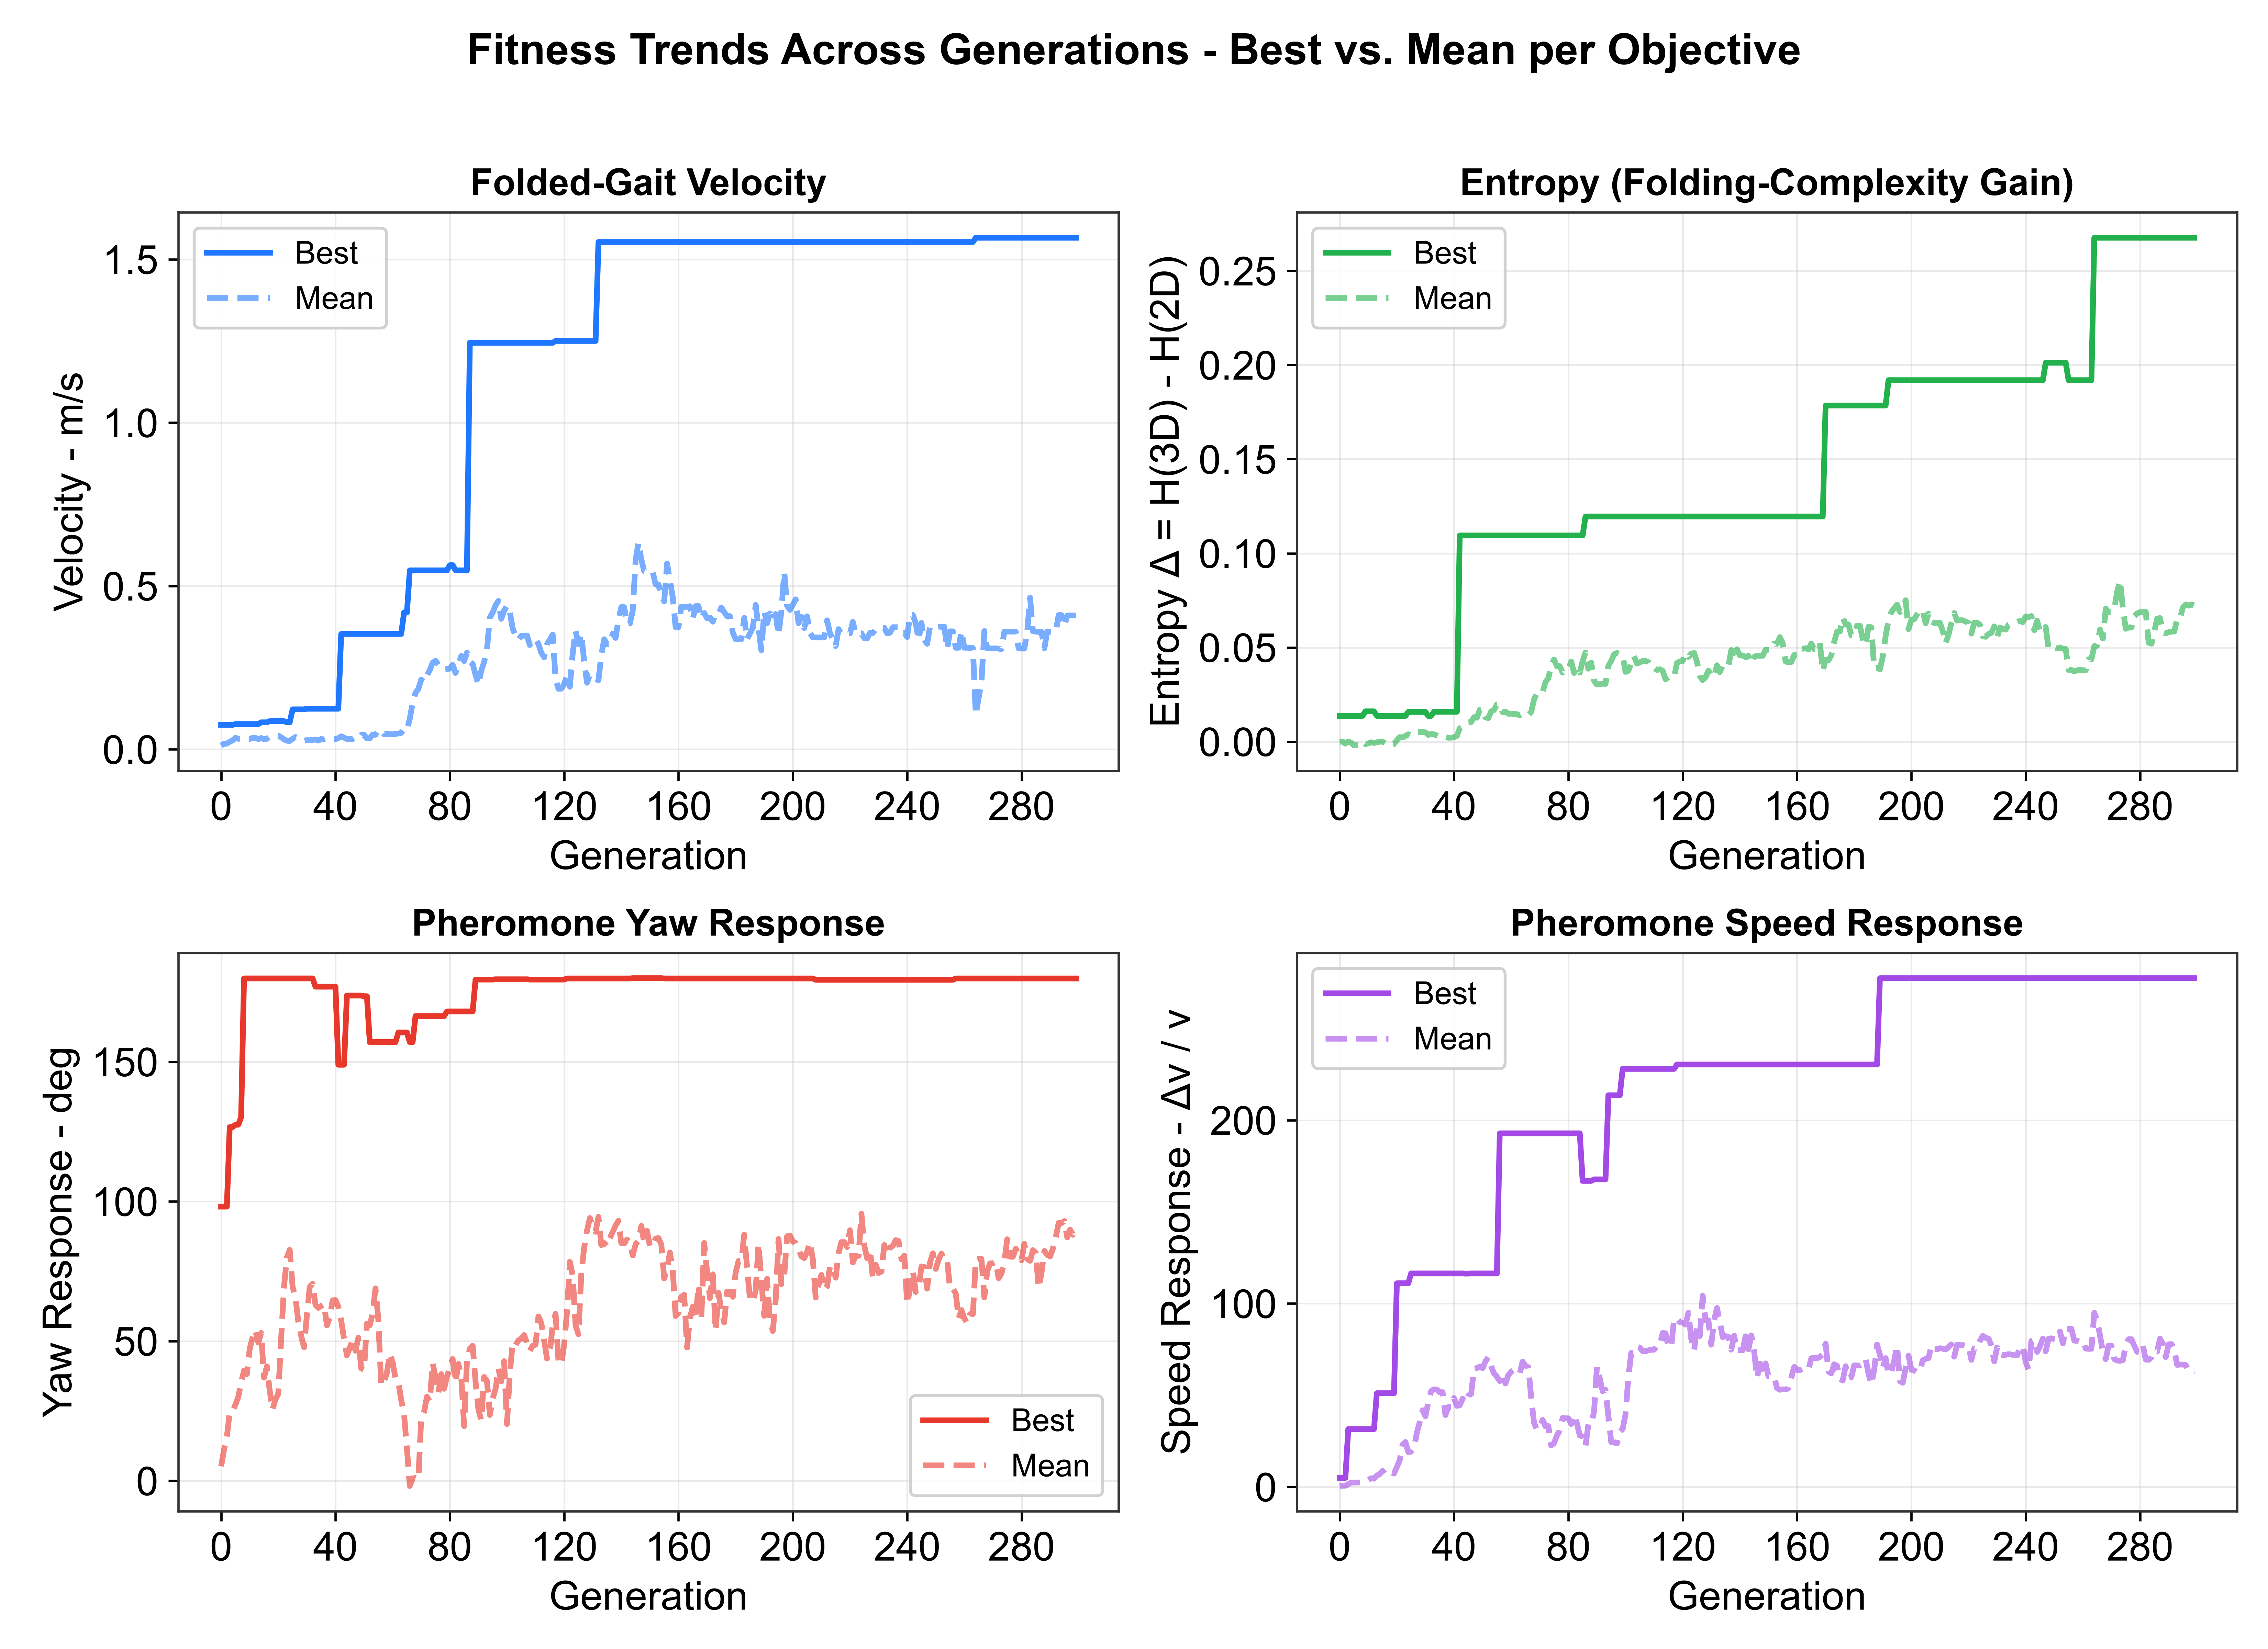
\includegraphics[width=\linewidth]{fitness_trends.png}
        \caption{Attractive configuration ($f_1$--$f_4$ all maximised).}
        \label{fig:fitness-trends}
    \end{subfigure}
    \par\vspace{0.6em}
    \begin{subfigure}[b]{\linewidth}
        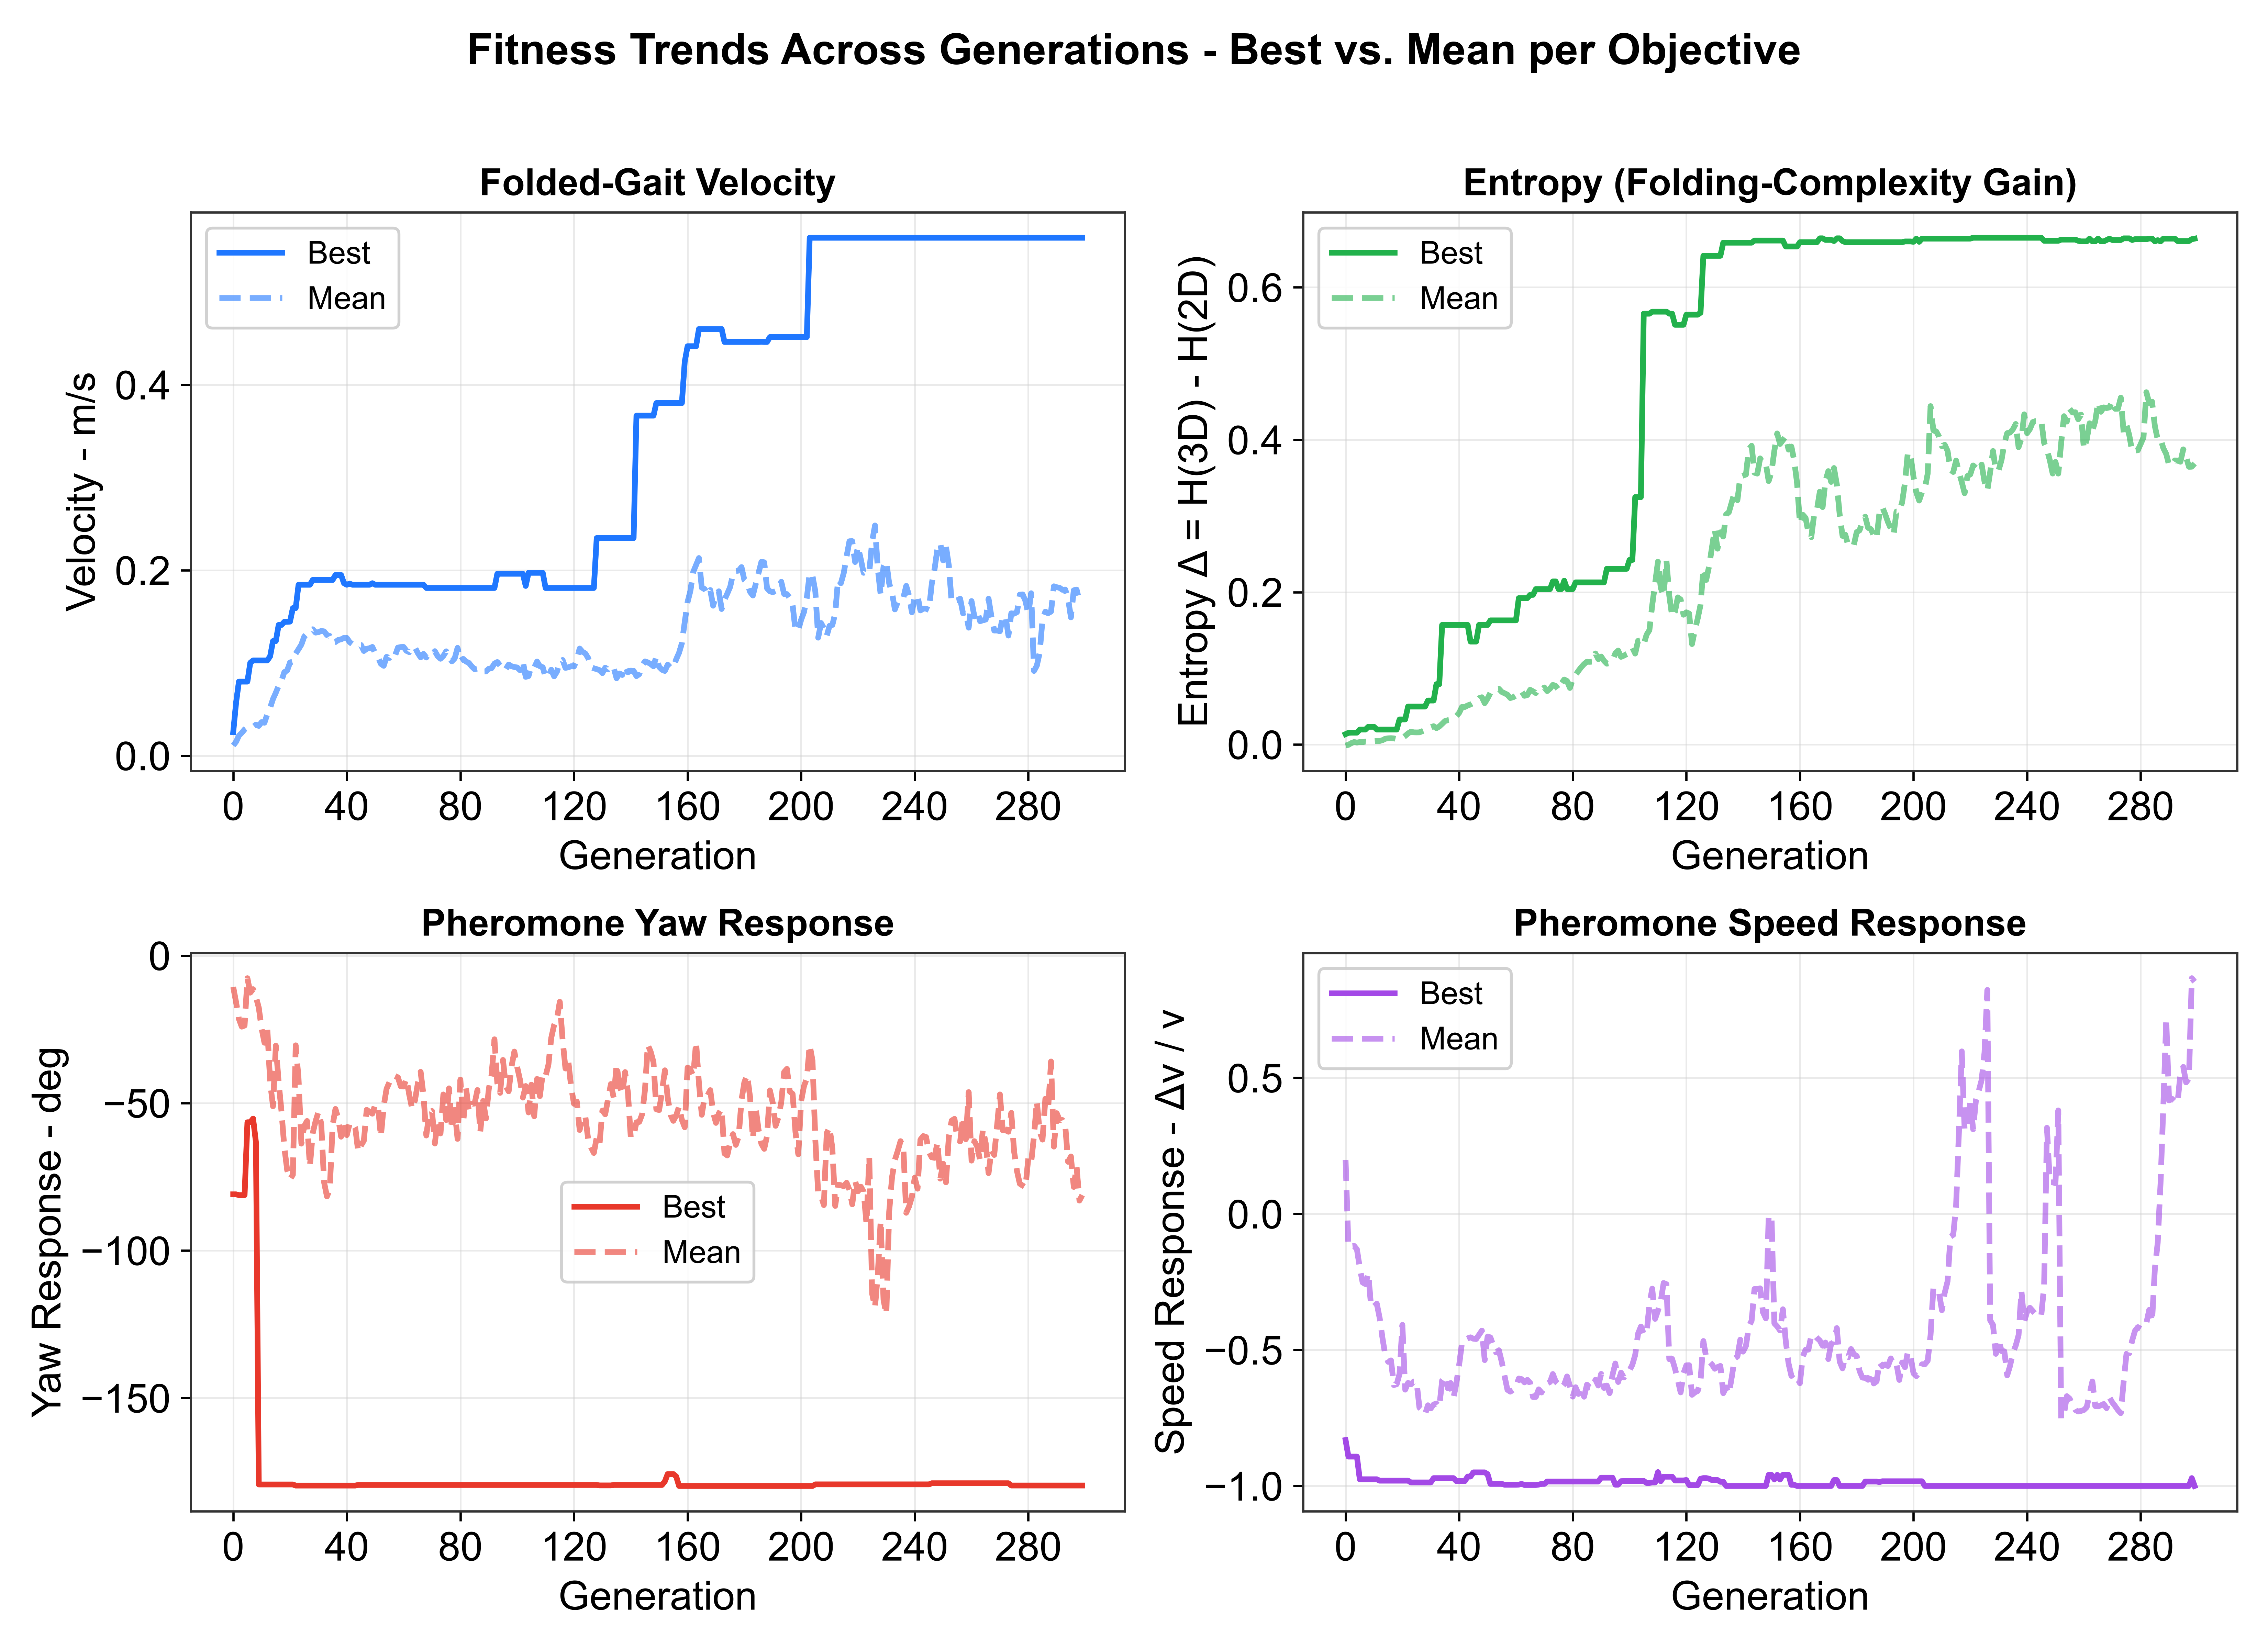
\includegraphics[width=\linewidth]{fitness_trends_repulsive.png}
        \caption{Repulsive configuration ($f_3$, $f_4$ minimised instead).}
        \label{fig:fitness-trends-repulsive}
    \end{subfigure}
    \caption{Fitness trends: best and mean raw population fitness per objective across generations, attractive versus repulsive configuration.}
    \label{fig:fitness-trends-both}
\end{figure}
\begin{figure}[H]
    \centering
    \begin{subfigure}[b]{0.48\linewidth}
        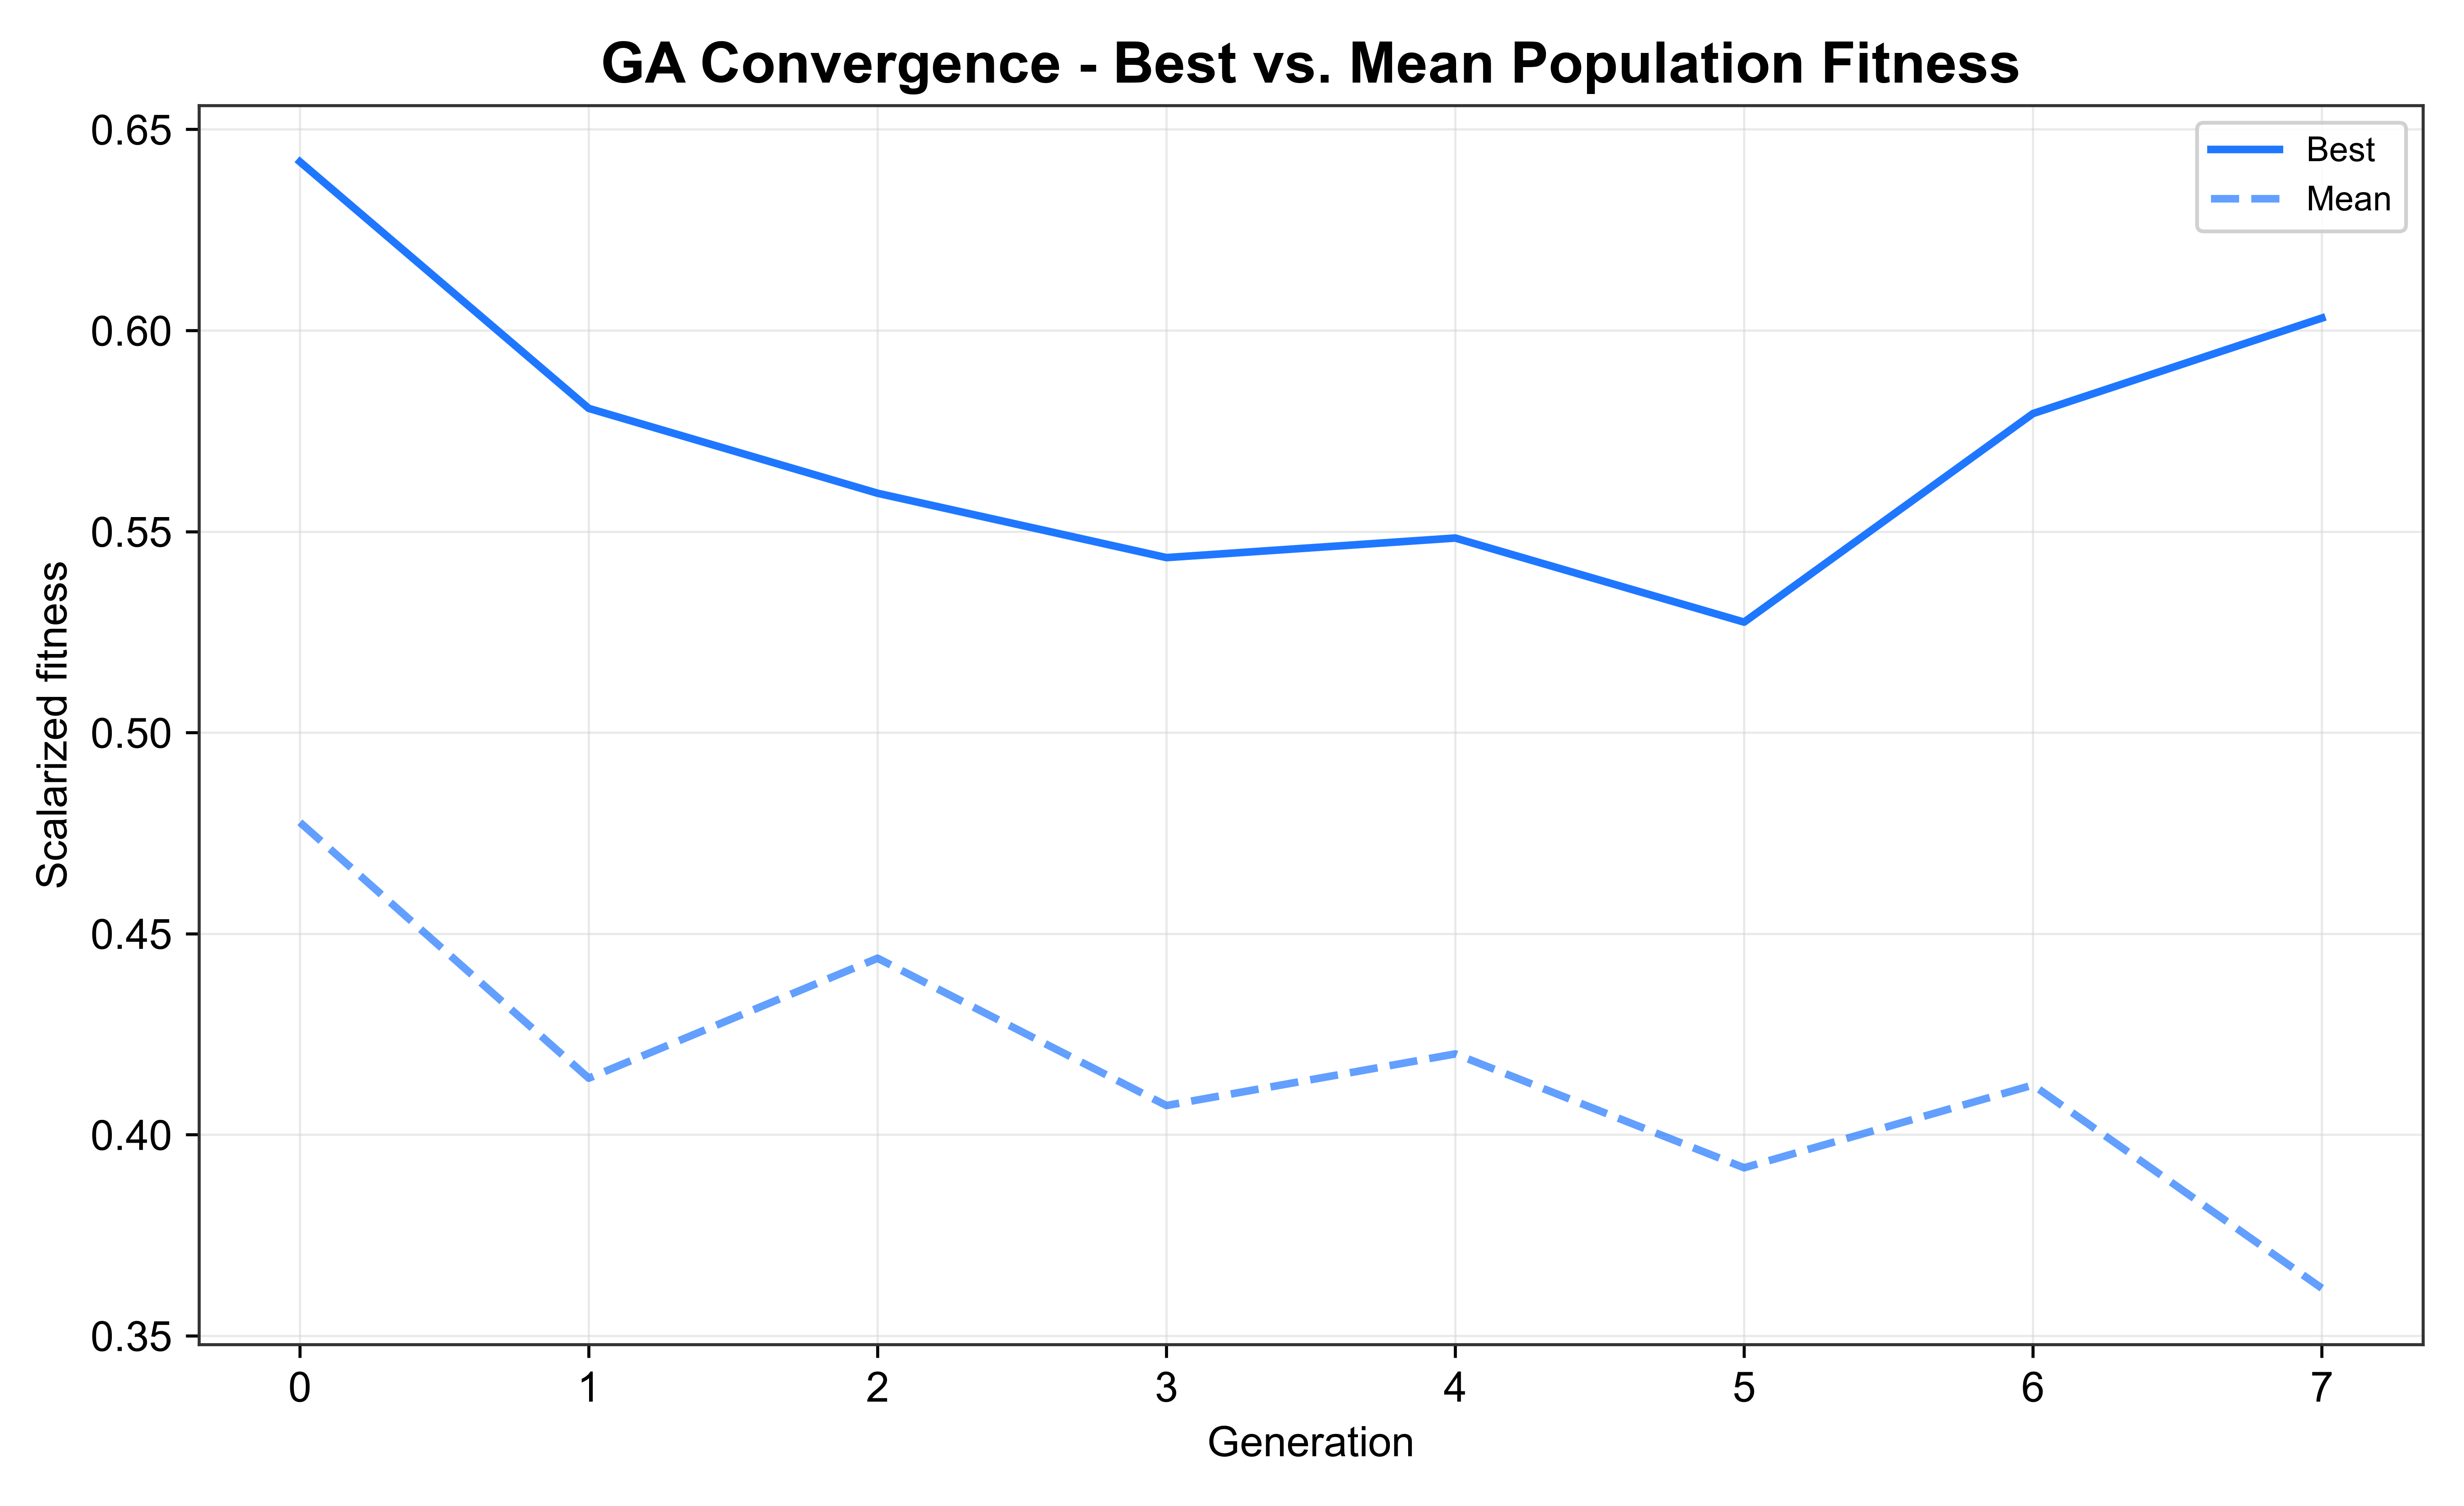
\includegraphics[width=\linewidth]{convergence.png}
        \caption{Attractive configuration.}
        \label{fig:convergence}
    \end{subfigure}
    \hfill
    \begin{subfigure}[b]{0.48\linewidth}
        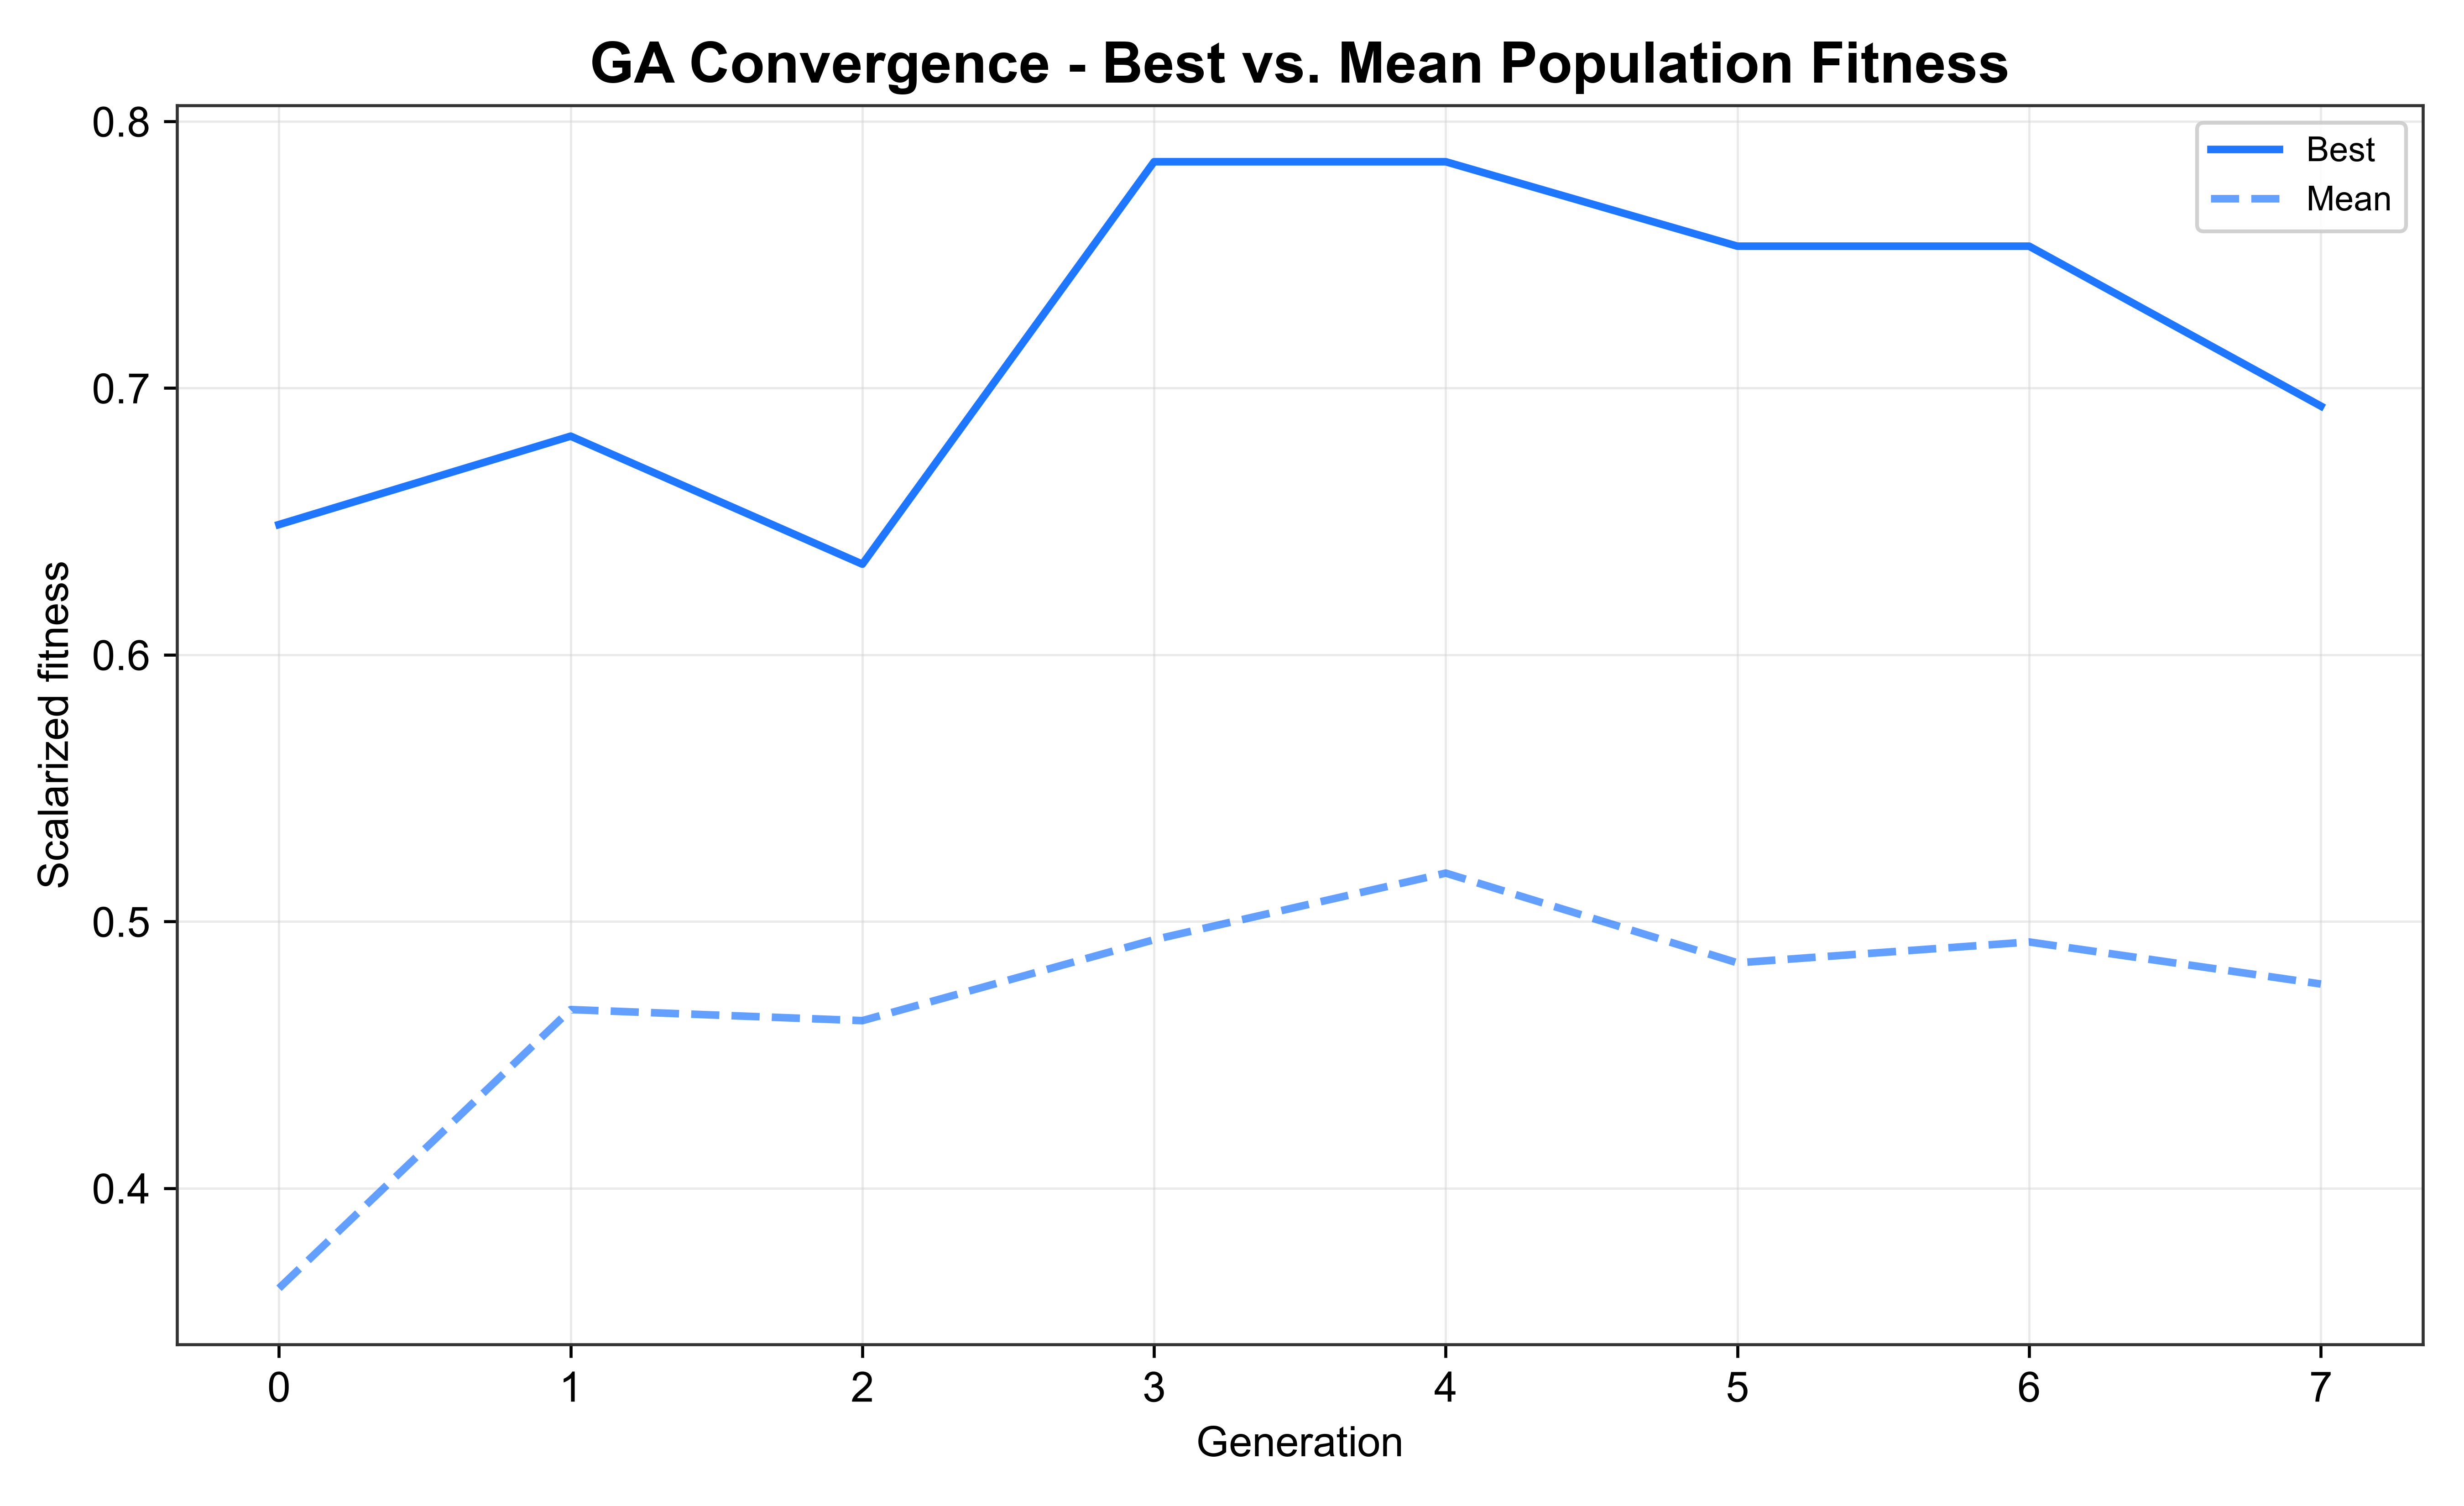
\includegraphics[width=\linewidth]{convergence_repulsive.png}
        \caption{Repulsive configuration.}
        \label{fig:convergence-repulsive}
    \end{subfigure}
    \caption{GA convergence: best and mean scalarized population fitness across generations, attractive versus repulsive configuration.}
    \label{fig:convergence-both}
\end{figure}
\begin{figure}[H]
    \centering
    \begin{subfigure}[b]{0.48\linewidth}
        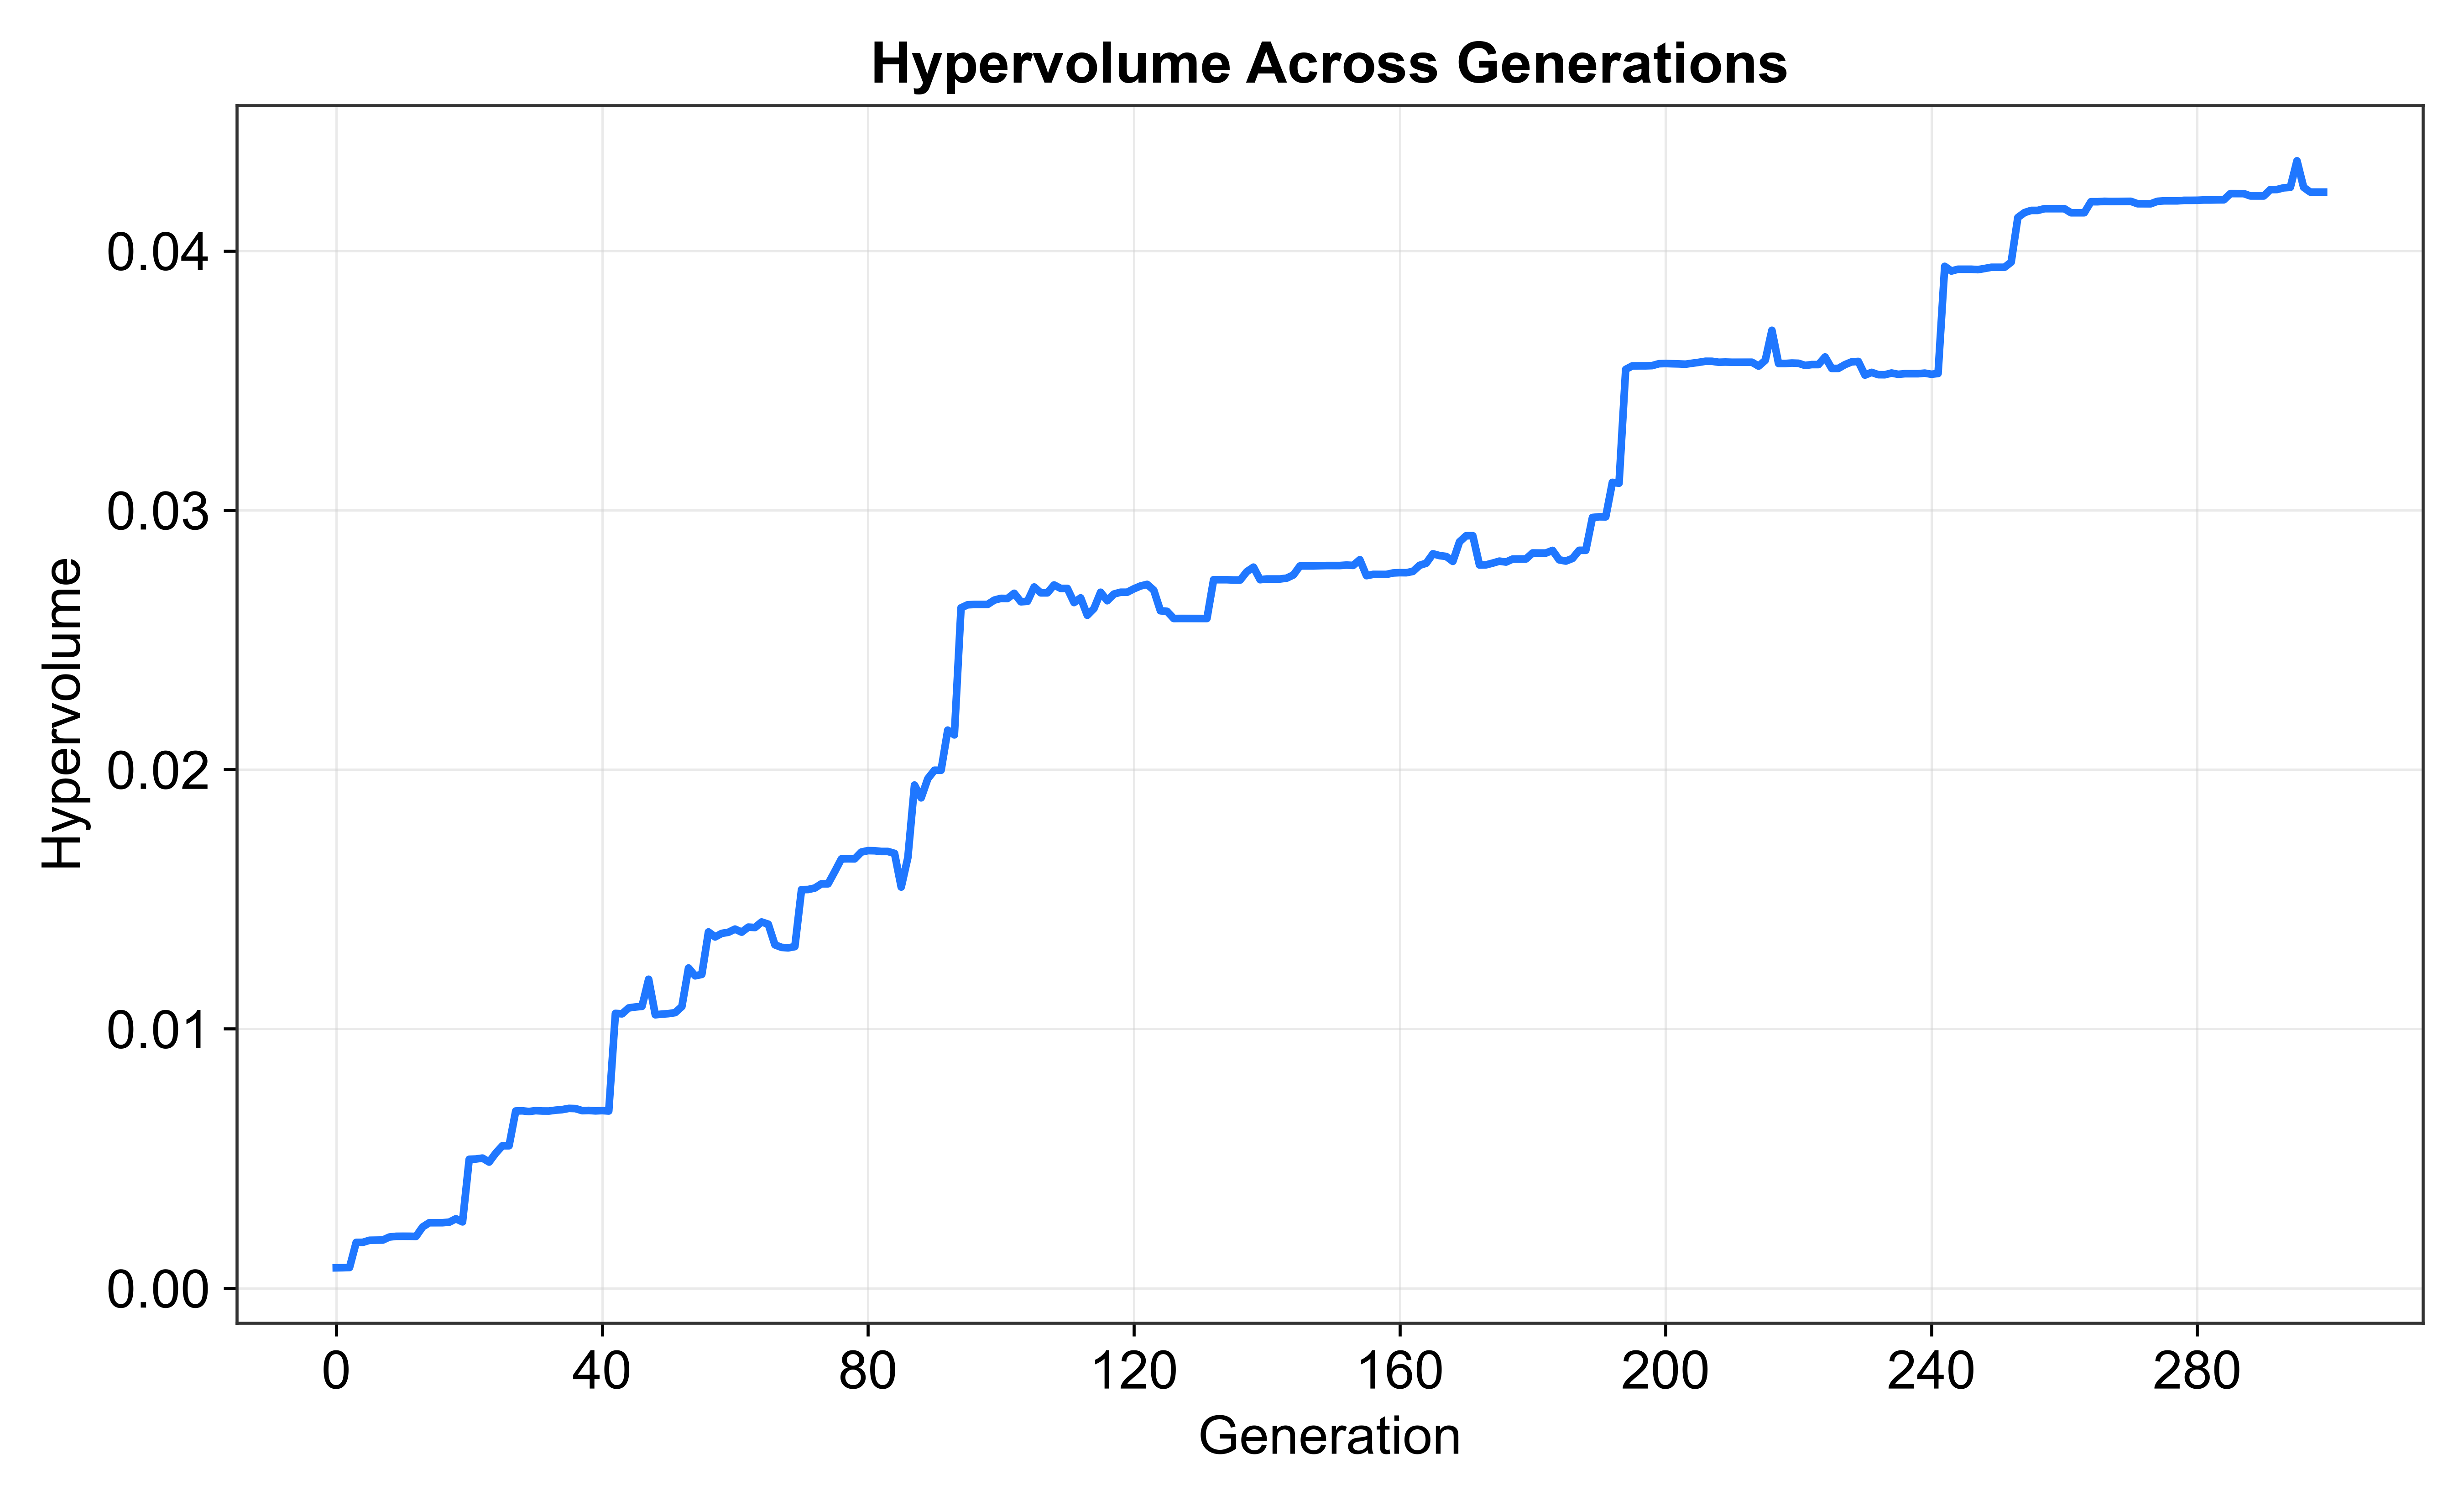
\includegraphics[width=\linewidth]{hypervolume.png}
        \caption{Attractive configuration.}
        \label{fig:hypervolume}
    \end{subfigure}
    \hfill
    \begin{subfigure}[b]{0.48\linewidth}
        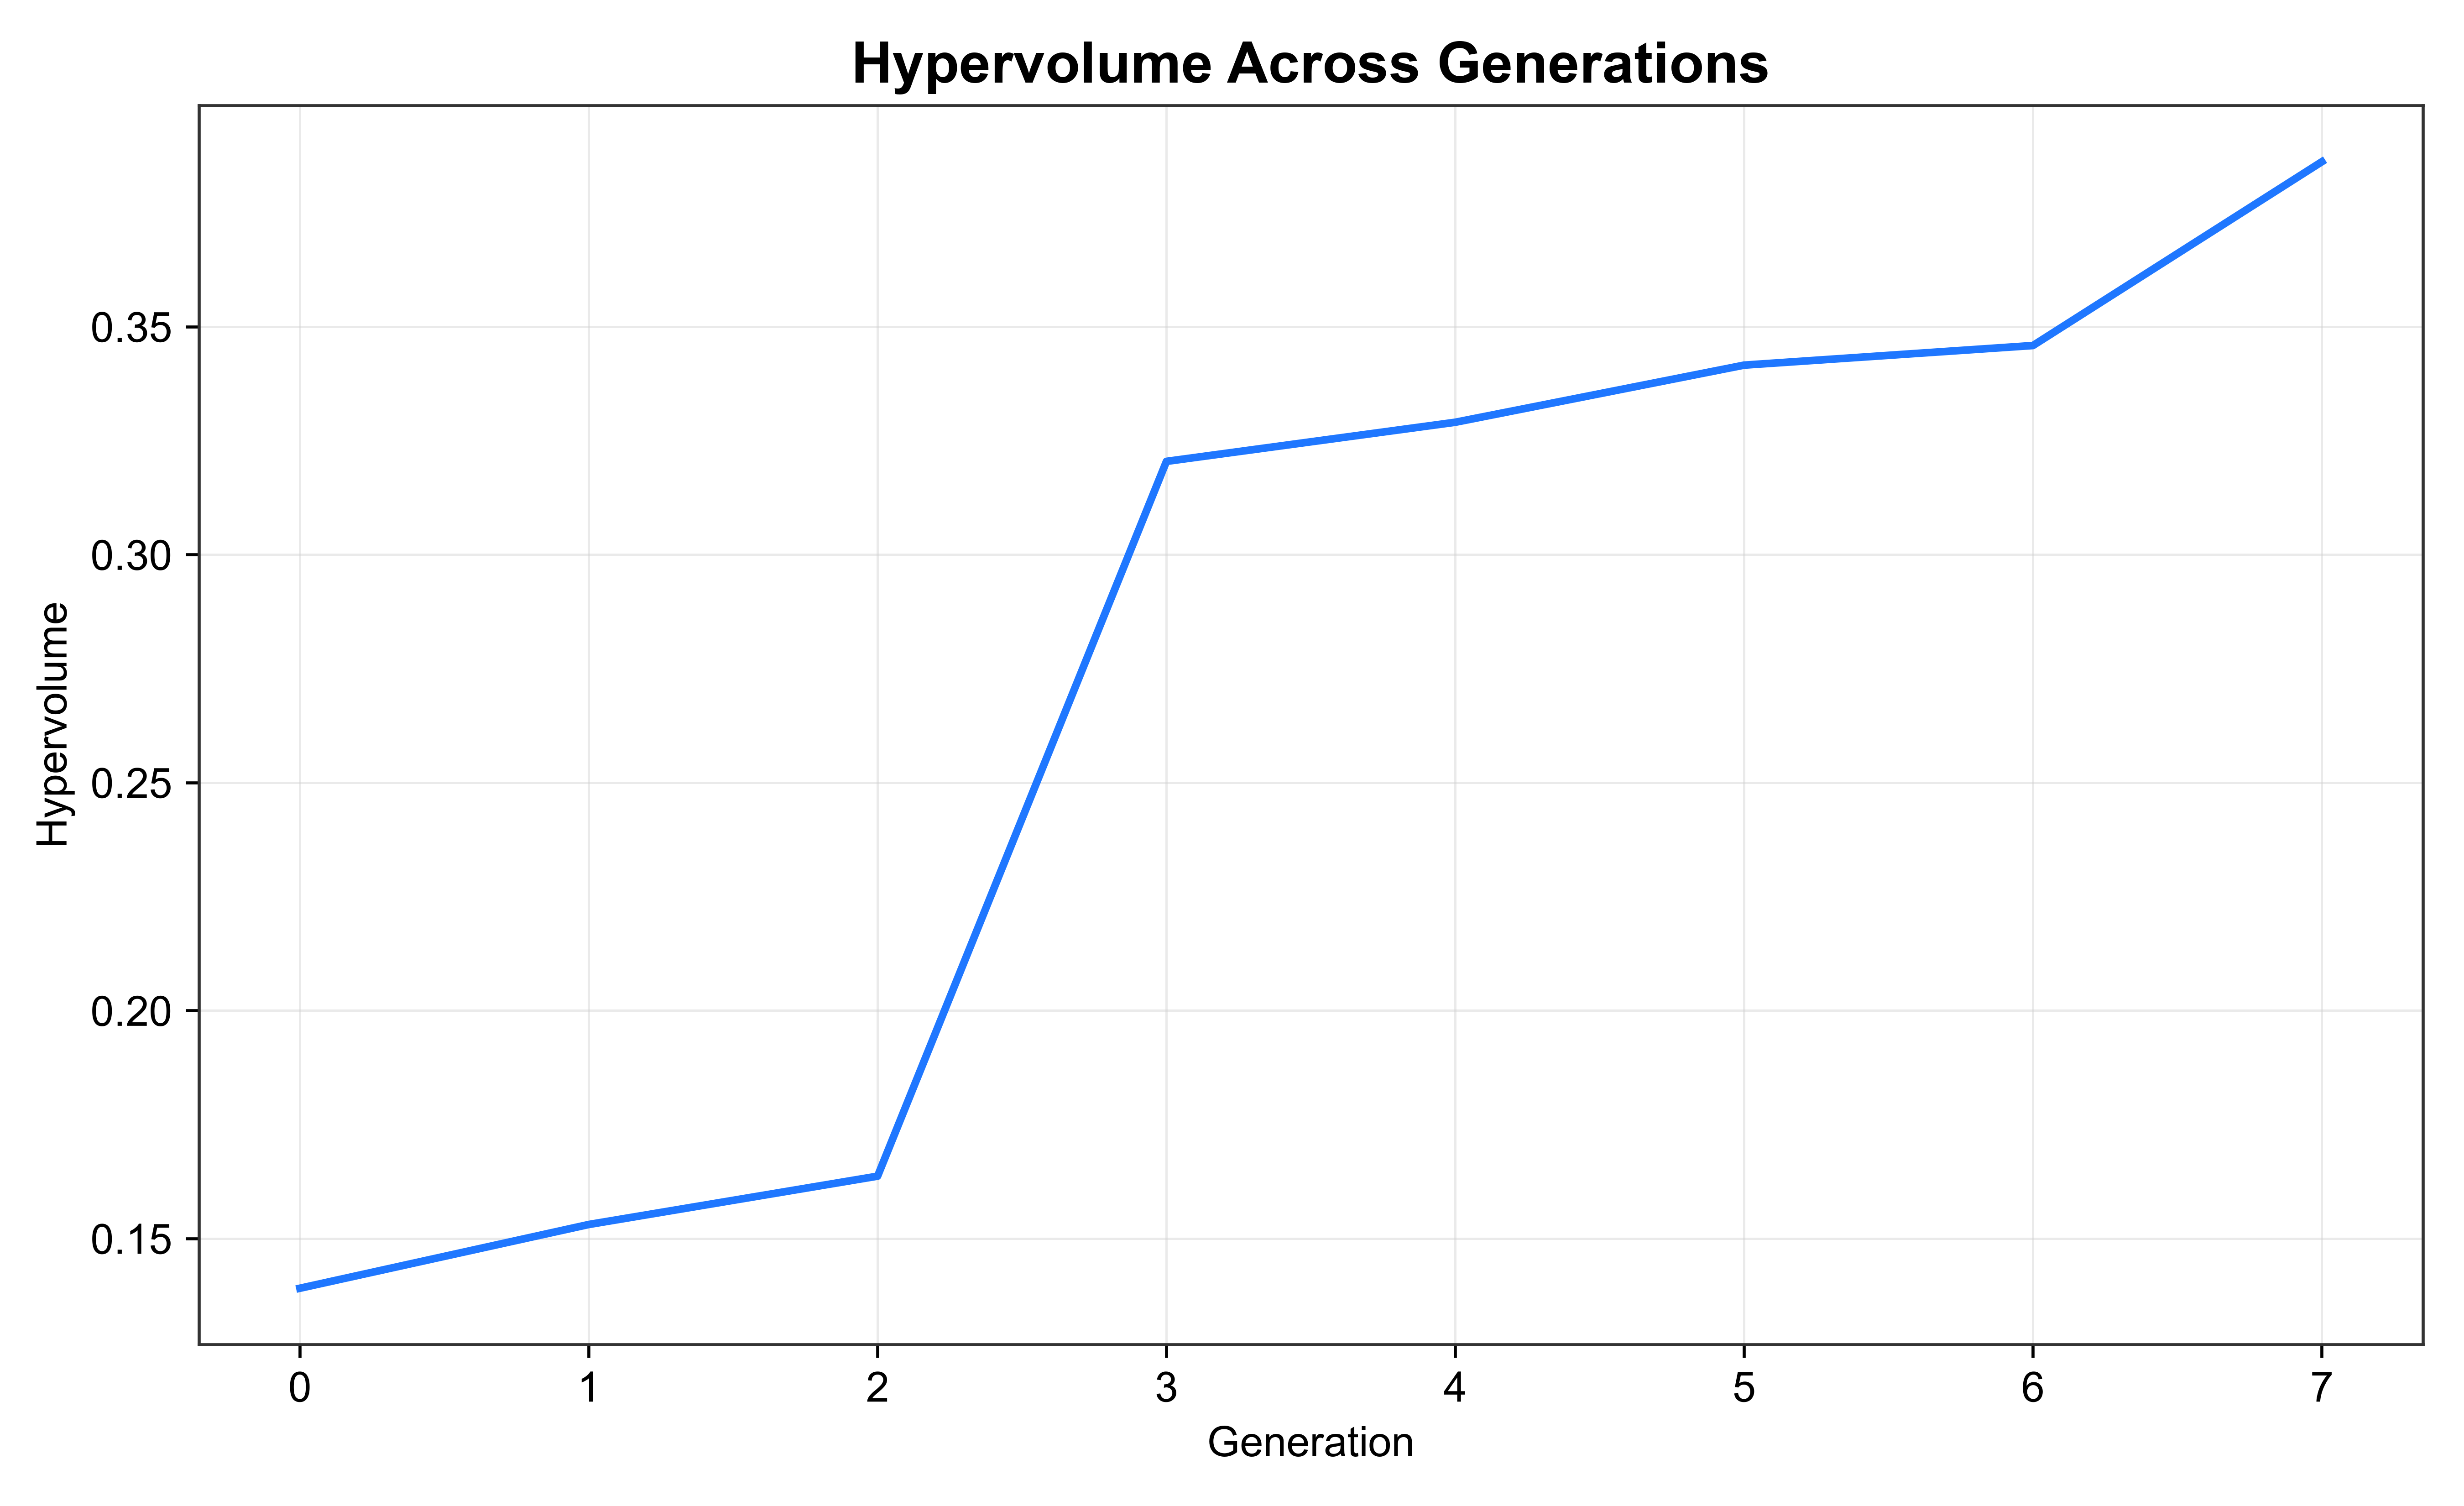
\includegraphics[width=\linewidth]{hypervolume_repulsive.png}
        \caption{Repulsive configuration.}
        \label{fig:hypervolume-repulsive}
    \end{subfigure}
    \caption{Hypervolume of the non-dominated front per generation, normalized against the run-wide objective range (Section~\ref{sec:eval-metrics}), attractive versus repulsive configuration.}
    \label{fig:hypervolume-both}
\end{figure}
Together, the scalarised fitness and hypervolume plots provide two views of progress. The scalarised curve gives a compact summary, whereas hypervolume considers improvement and spread across all four objectives. As shown in Fig.~\ref{fig:hypervolume}, hypervolume rises in a step-like, largely monotonic pattern across the full 300-generation run, from close to zero to approximately 0.042, with the largest single steps around generations 90--95, 190--195 and 240--250 and a further rise still visible at the final generations recorded; it had not visibly plateaued by the end of the run. The four per-objective best-individual curves in Fig.~\ref{fig:fitness-trends} converge on different schedules: folded-gait velocity and yaw response reach a stable plateau by around generation 90--130, whereas entropy gain and speed response continue increasing in steps through most of the run and are still rising at its end. The scalarised best-fitness curve in Fig.~\ref{fig:convergence} is less monotonic than hypervolume -- it peaks around generation 55, falls back over the following generations, and settles into a lower band for most of the run -- which is expected because scalarisation compresses four objectives with different convergence schedules into one number and can fall even while hypervolume, which tracks the whole non-dominated set rather than one scalar, continues to rise. This supports the implementation of the evolutionary loop and gives evidence for O-4: the population is still visibly improving in aggregate (hypervolume) after 300 generations, so a longer run cannot be ruled out from steadying the result further, consistent with the point raised in Section~\ref{ch:conclusion}.

\section{Pareto Front and Trade-off Analysis}
\label{sec:pareto-results}
\begin{figure}[H]
    \centering
    \begin{subfigure}[b]{\linewidth}
        \centering
        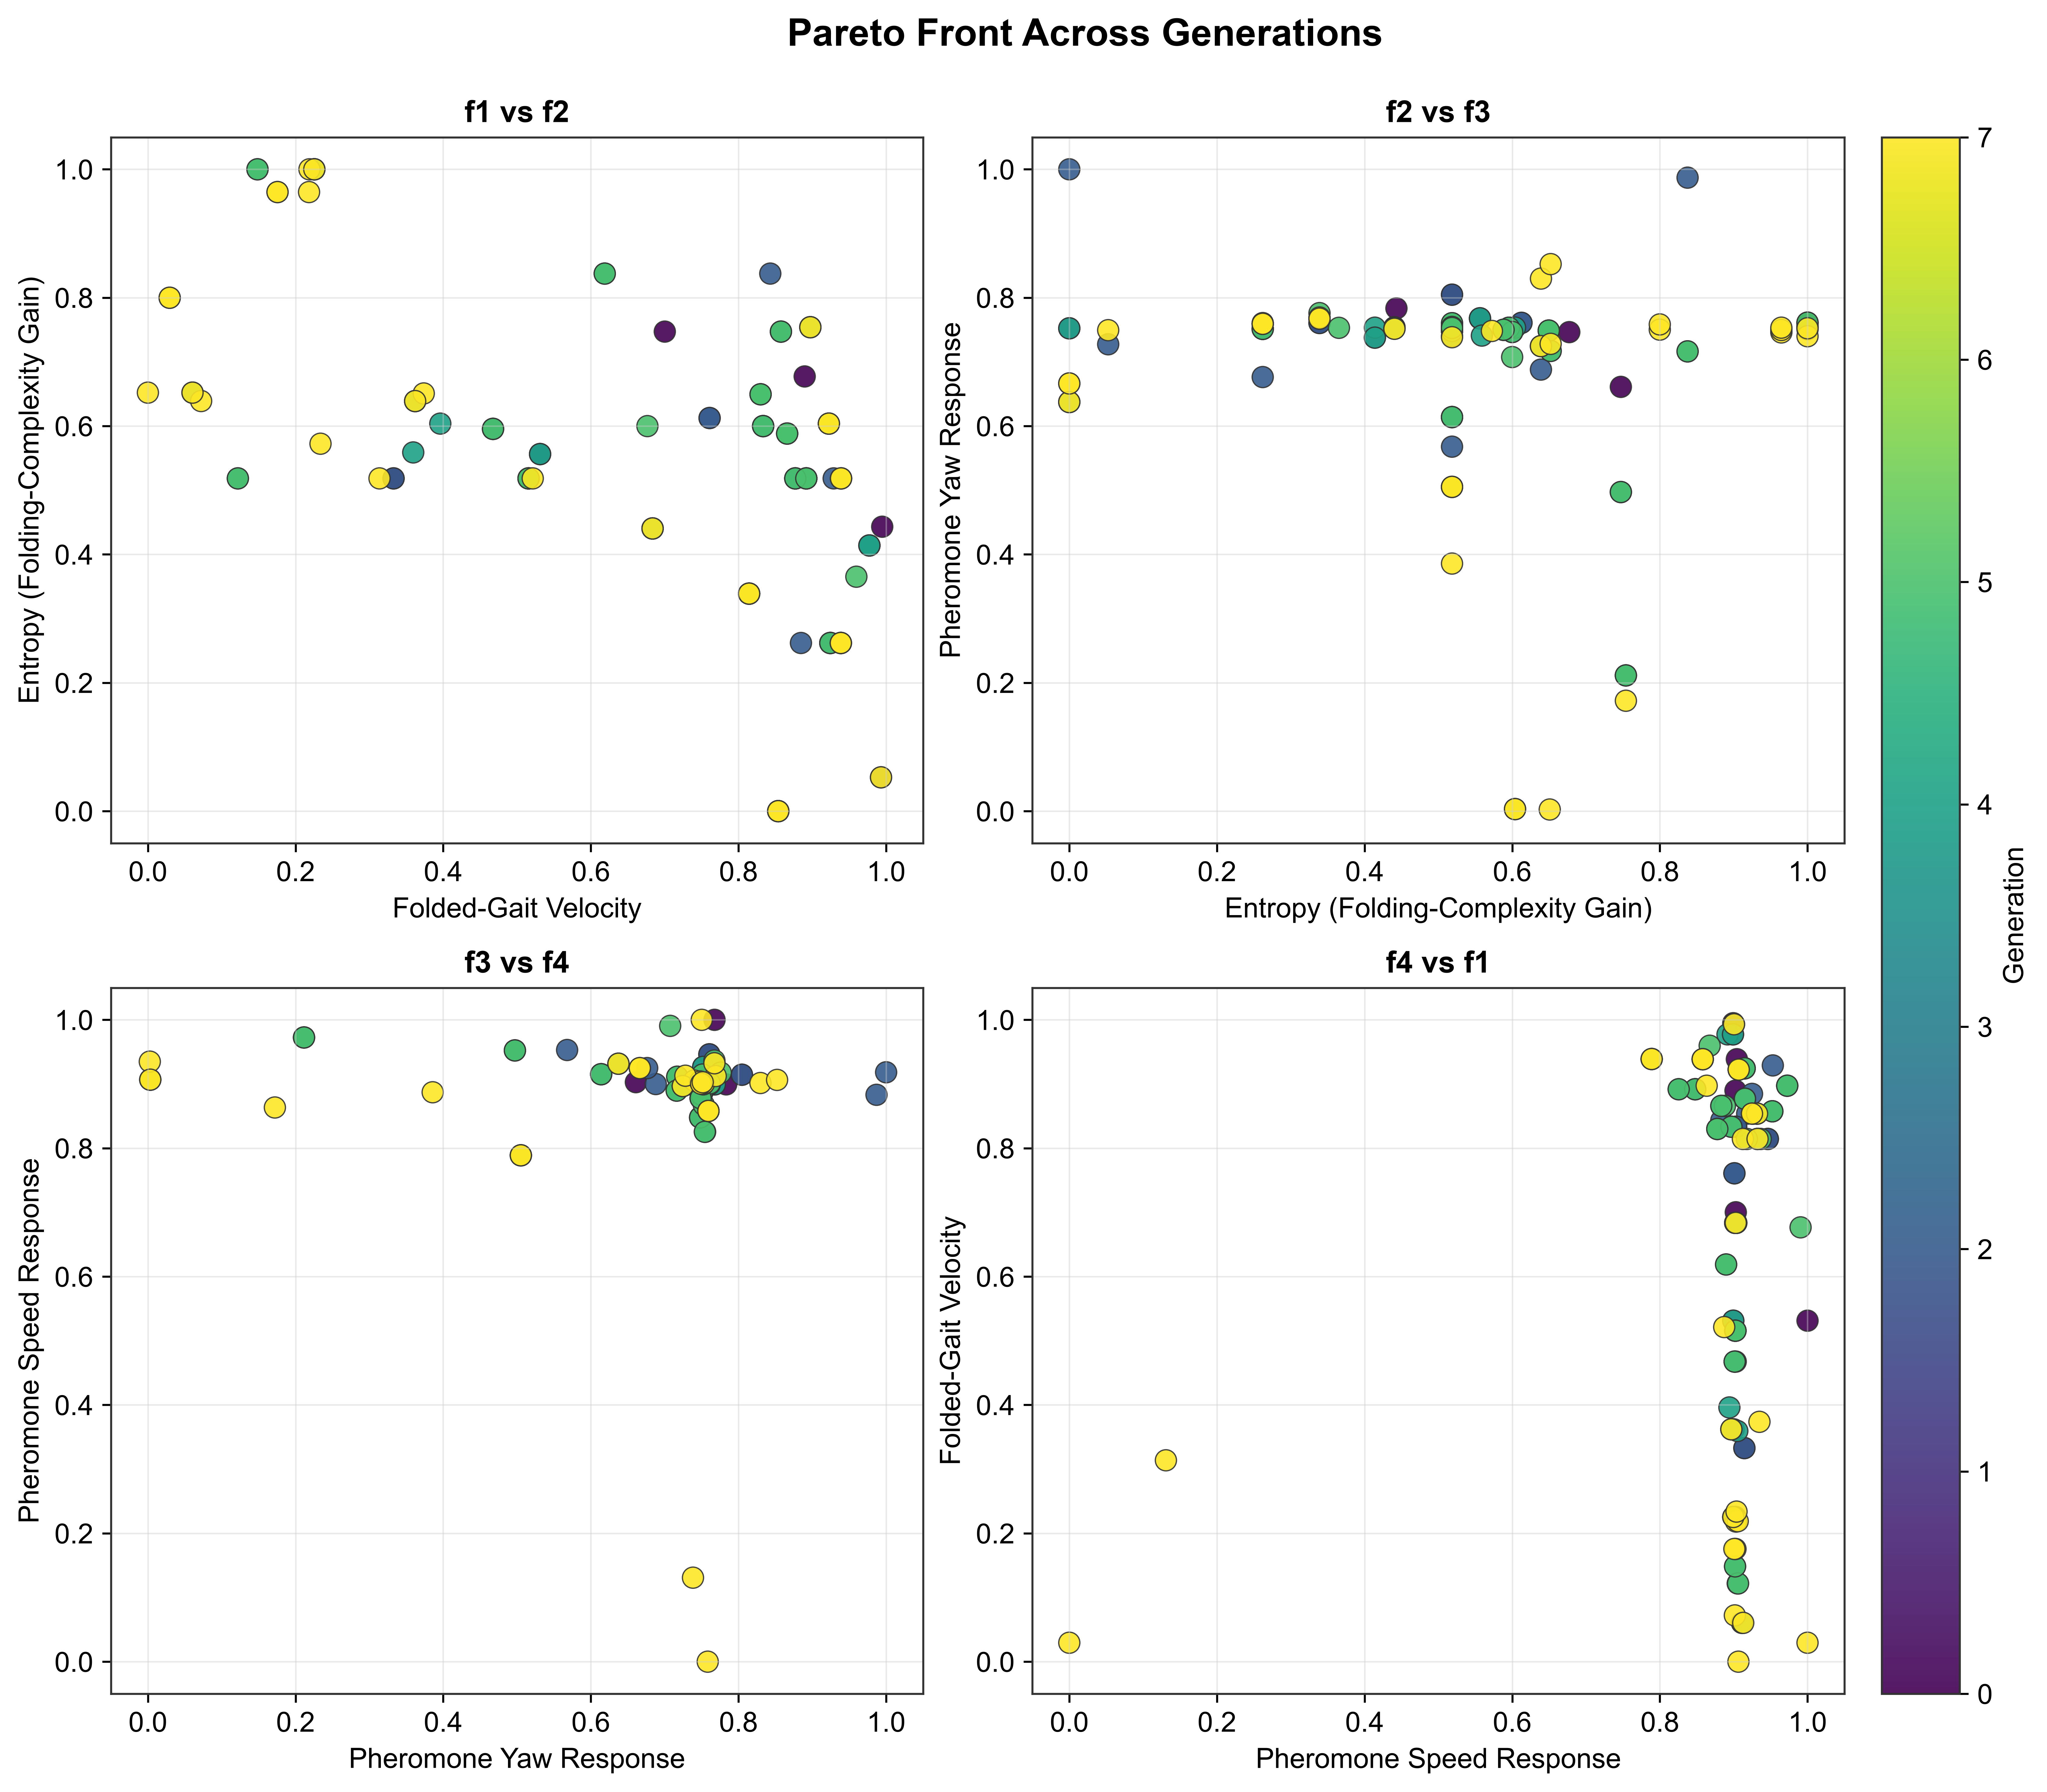
\includegraphics[width=0.6\linewidth]{pareto_front.png}
        \caption{Attractive configuration.}
        \label{fig:pareto-front}
    \end{subfigure}
    \par\vspace{0.6em}
    \begin{subfigure}[b]{\linewidth}
        \centering
        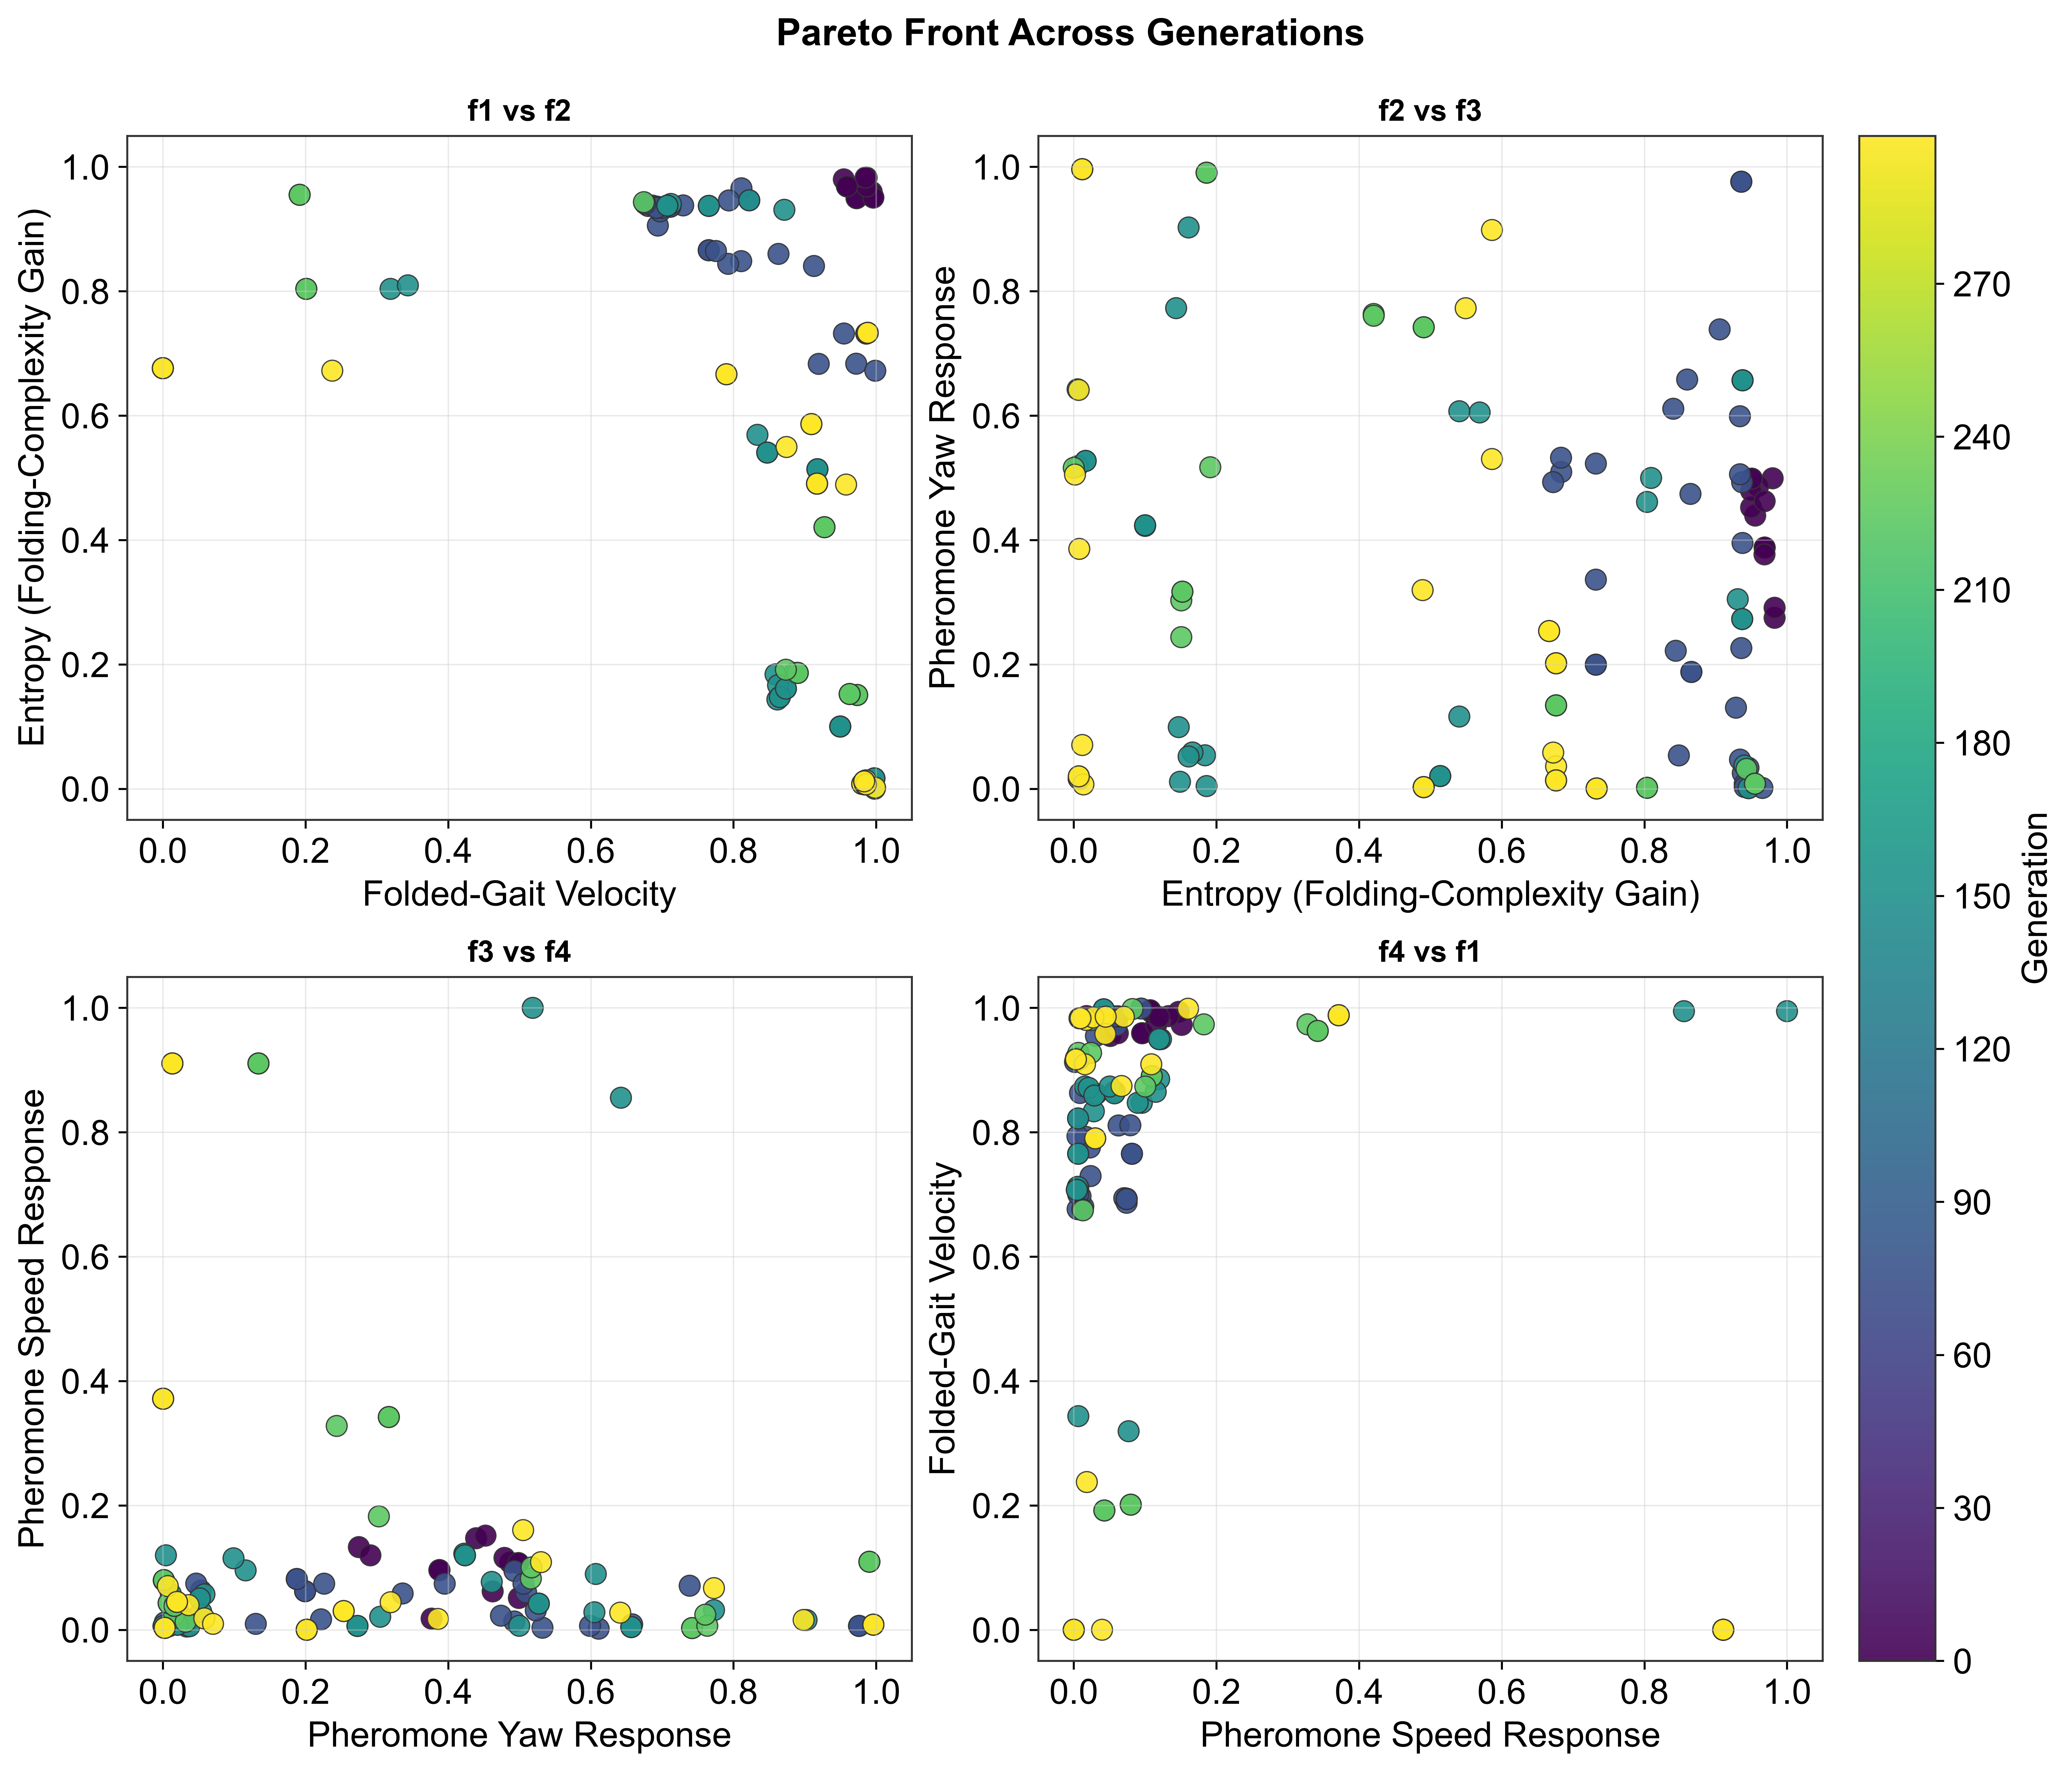
\includegraphics[width=0.6\linewidth]{pareto_front_repulsive.png}
        \caption{Repulsive configuration ($f_3$, $f_4$ minimised).}
        \label{fig:pareto-front-repulsive}
    \end{subfigure}
    \caption{Non-dominated individuals recorded across the run, pairwise across all four objectives ($f_1$ vs $f_2$, $f_2$ vs $f_3$, $f_3$ vs $f_4$, $f_4$ vs $f_1$; axes min-max normalized), coloured by generation, attractive versus repulsive configuration.}
    \label{fig:pareto-front-both}
\end{figure}
The recorded non-dominated set contains solutions with different compromises between speed, folding complexity and light response. A four-objective problem can produce many non-dominated individuals because one candidate may be better in one objective and worse in another. This dominance resistance is expected for a modest population and should not be interpreted as proof that all designs are equally useful. As shown in the $f_1$ vs $f_2$ panel of Fig.~\ref{fig:pareto-front}, most non-dominated individuals cluster at high folded-gait velocity with either high or near-zero entropy gain, rather than at intermediate values of both -- consistent with a trade-off in which a design tends to specialise toward fast locomotion or toward folding complexity rather than combining both to a moderate degree. The $f_3$ vs $f_4$ panel shows the great majority of points already saturated near the maximum recorded speed response regardless of yaw response, so speed response is rarely the binding constraint on this front. Point colour (generation) is spread across the full run in every panel, indicating that the non-dominated set is populated by individuals recorded throughout the run rather than only in its final generations.

\section{Morphological Complexity versus Locomotion}
\label{sec:entropy-velocity}
\begin{figure}[H]
    \centering
    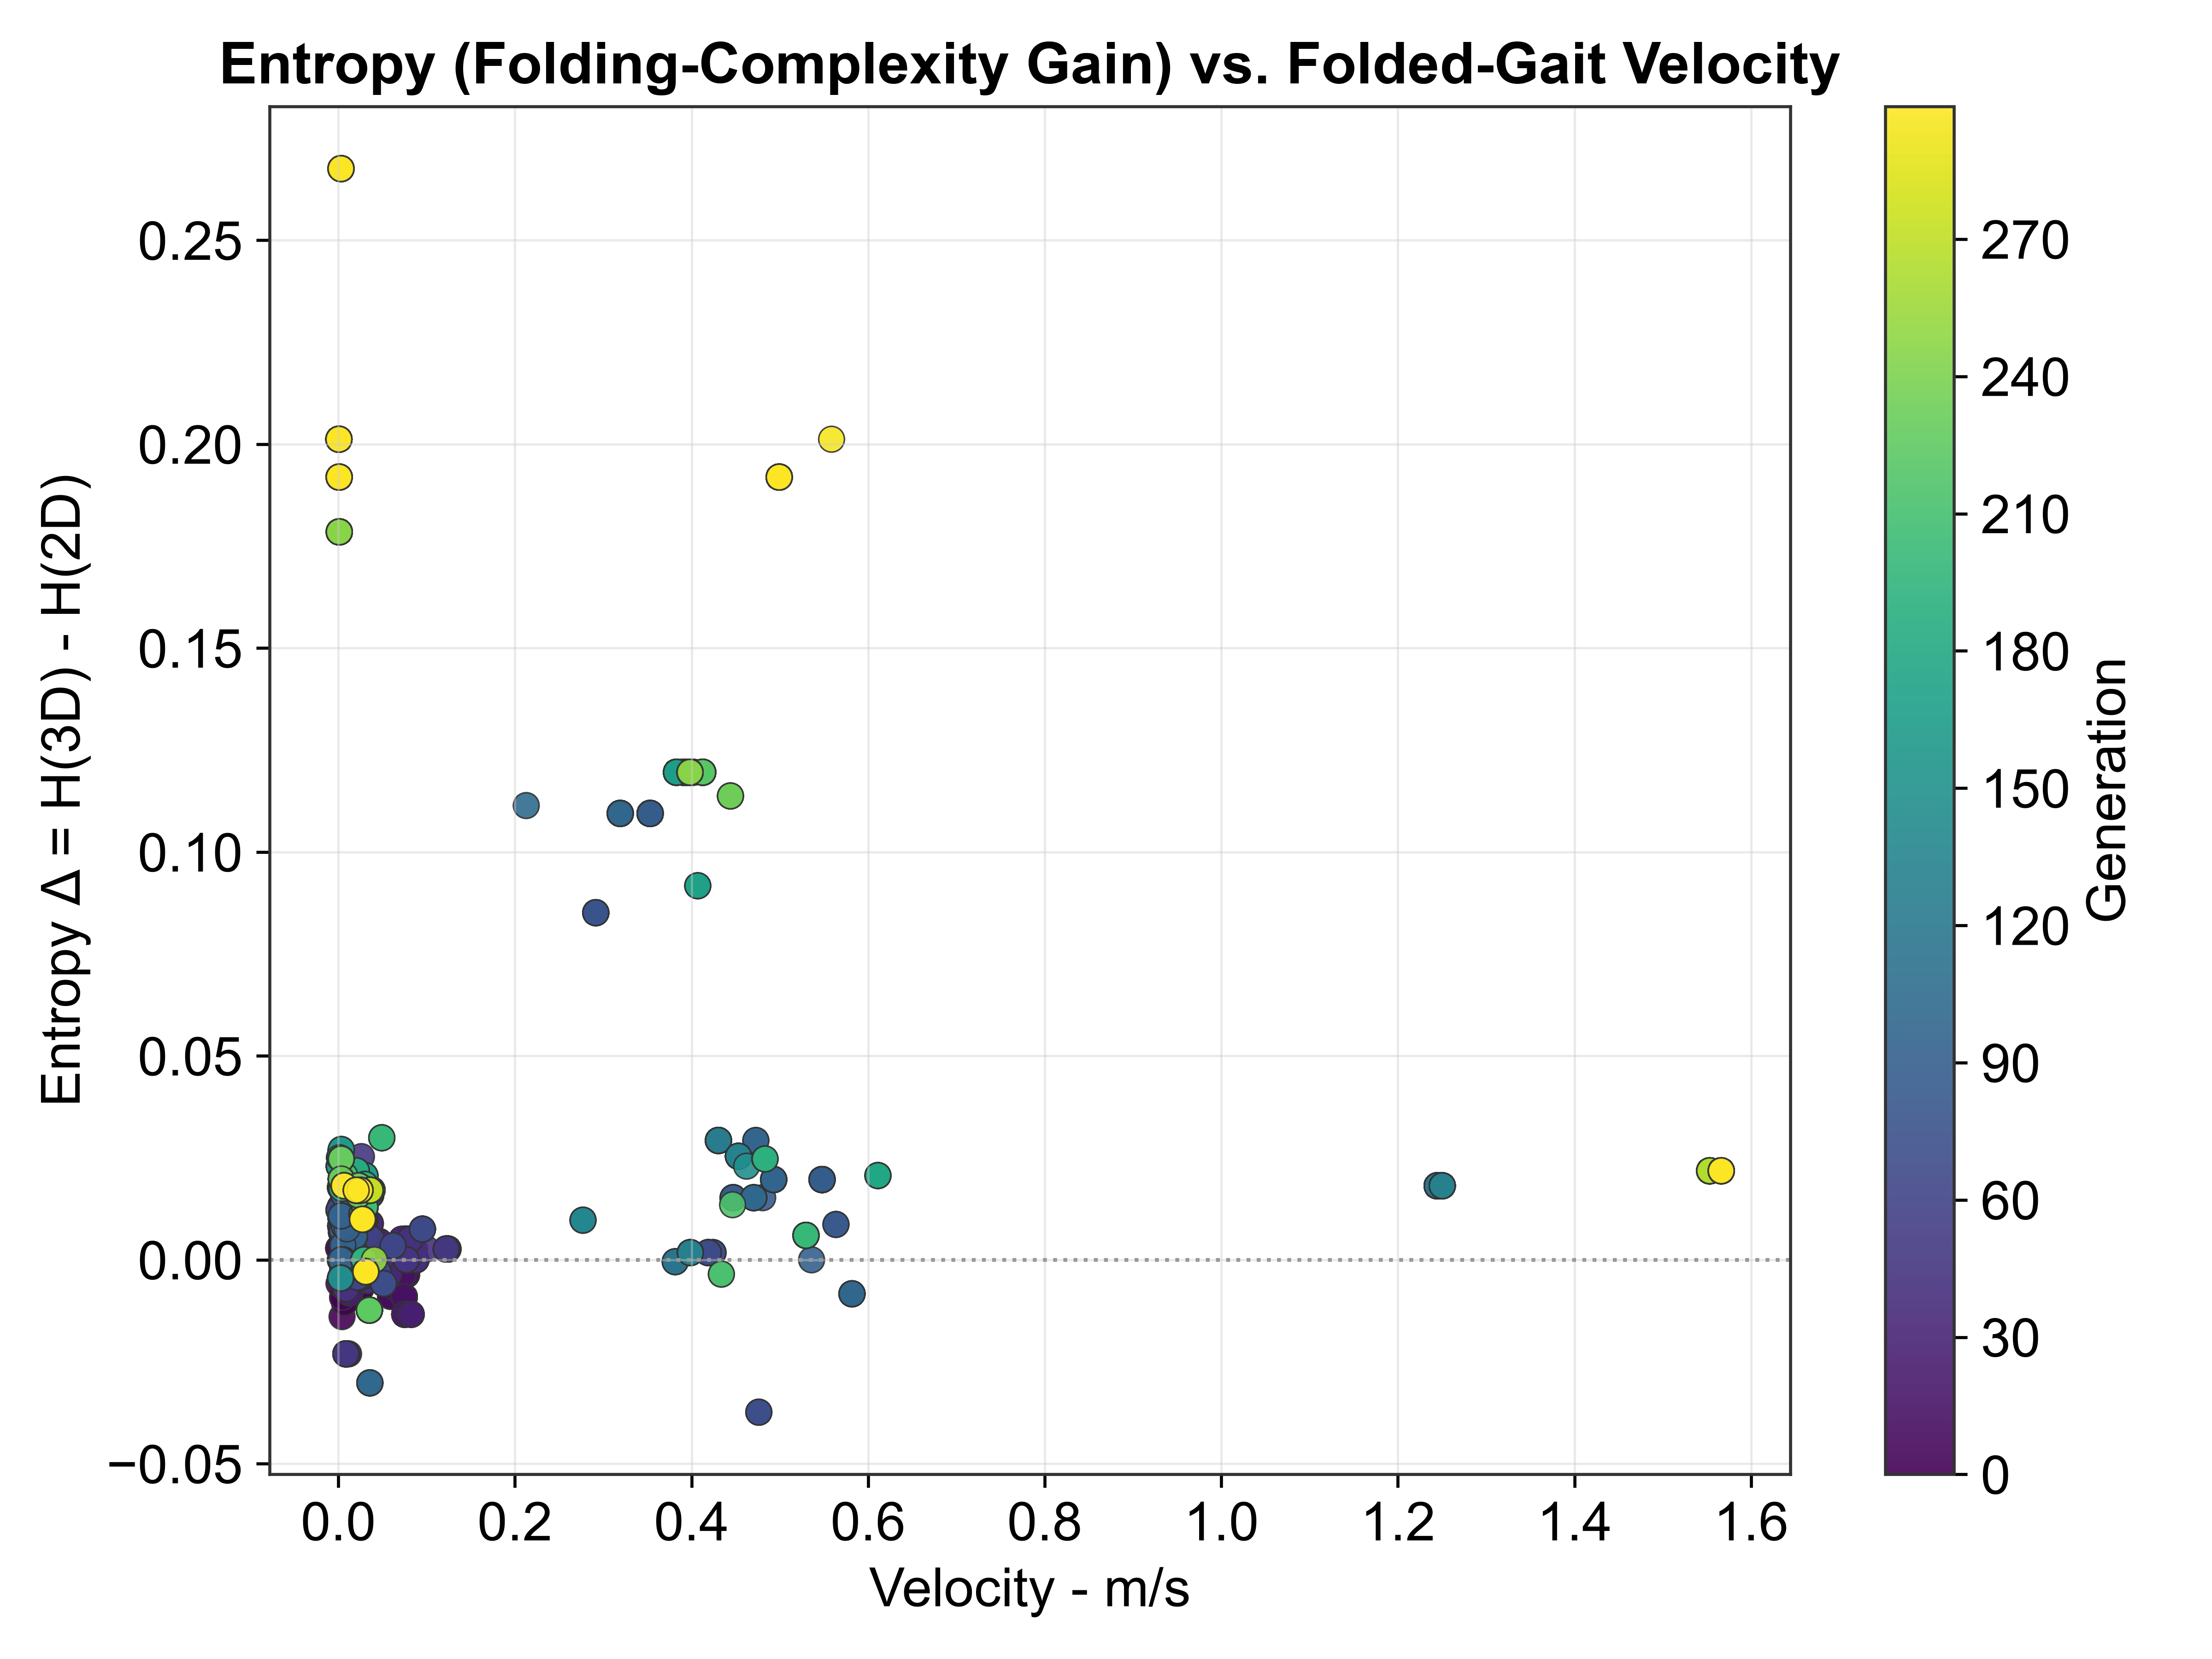
\includegraphics[width=0.85\linewidth]{entropy_vs_velocity.png}
    \caption{Folding-complexity gain ($f_2$) versus folded-gait velocity ($f_1$), all individuals across all generations, coloured by generation.}
    \label{fig:entropy-velocity}
\end{figure}
The entropy--velocity plot addresses AO-2 by comparing a measure of change during folding with the resulting gait speed. As shown in Fig.~\ref{fig:entropy-velocity}, the individuals with the highest entropy gain ($\Delta H \gtrsim 0.18$) are concentrated at near-zero velocity, with two exceptions from late generations (indicated by point colour) that combine a comparable entropy gain ($\Delta H \approx 0.19$--$0.20$) with a moderate velocity of around 0.5\,m/s. Conversely, the two highest-velocity individuals recorded (around 1.25 and 1.55\,m/s) both have a low entropy gain close to 0.02. The bulk of the population sits at low-to-moderate velocity (0--0.6\,m/s) with a low entropy gain (0--0.03). This pattern is consistent with a trade-off in which high folding-complexity gain is difficult to combine with fast locomotion, though the two late-generation counterexamples show the trade-off is not absolute -- and, since these are the only two points recorded at that combination, this remains a case of a small number of specific designs rather than a general rule established by the run. A broad low-entropy cloud spanning most of the observed velocity range would suggest that connectivity and actuation choices dominate velocity regardless of folding complexity, and the low-entropy majority described above is consistent with that as well. The available evidence supports examining the relationship, but it does not justify a causal claim, and no statistical test of association has been applied to these data.

\section{Evolved Morphologies: Attractive and Repulsive Response}
\label{sec:evolved-morphologies}
\begin{figure}[H]
    \centering
    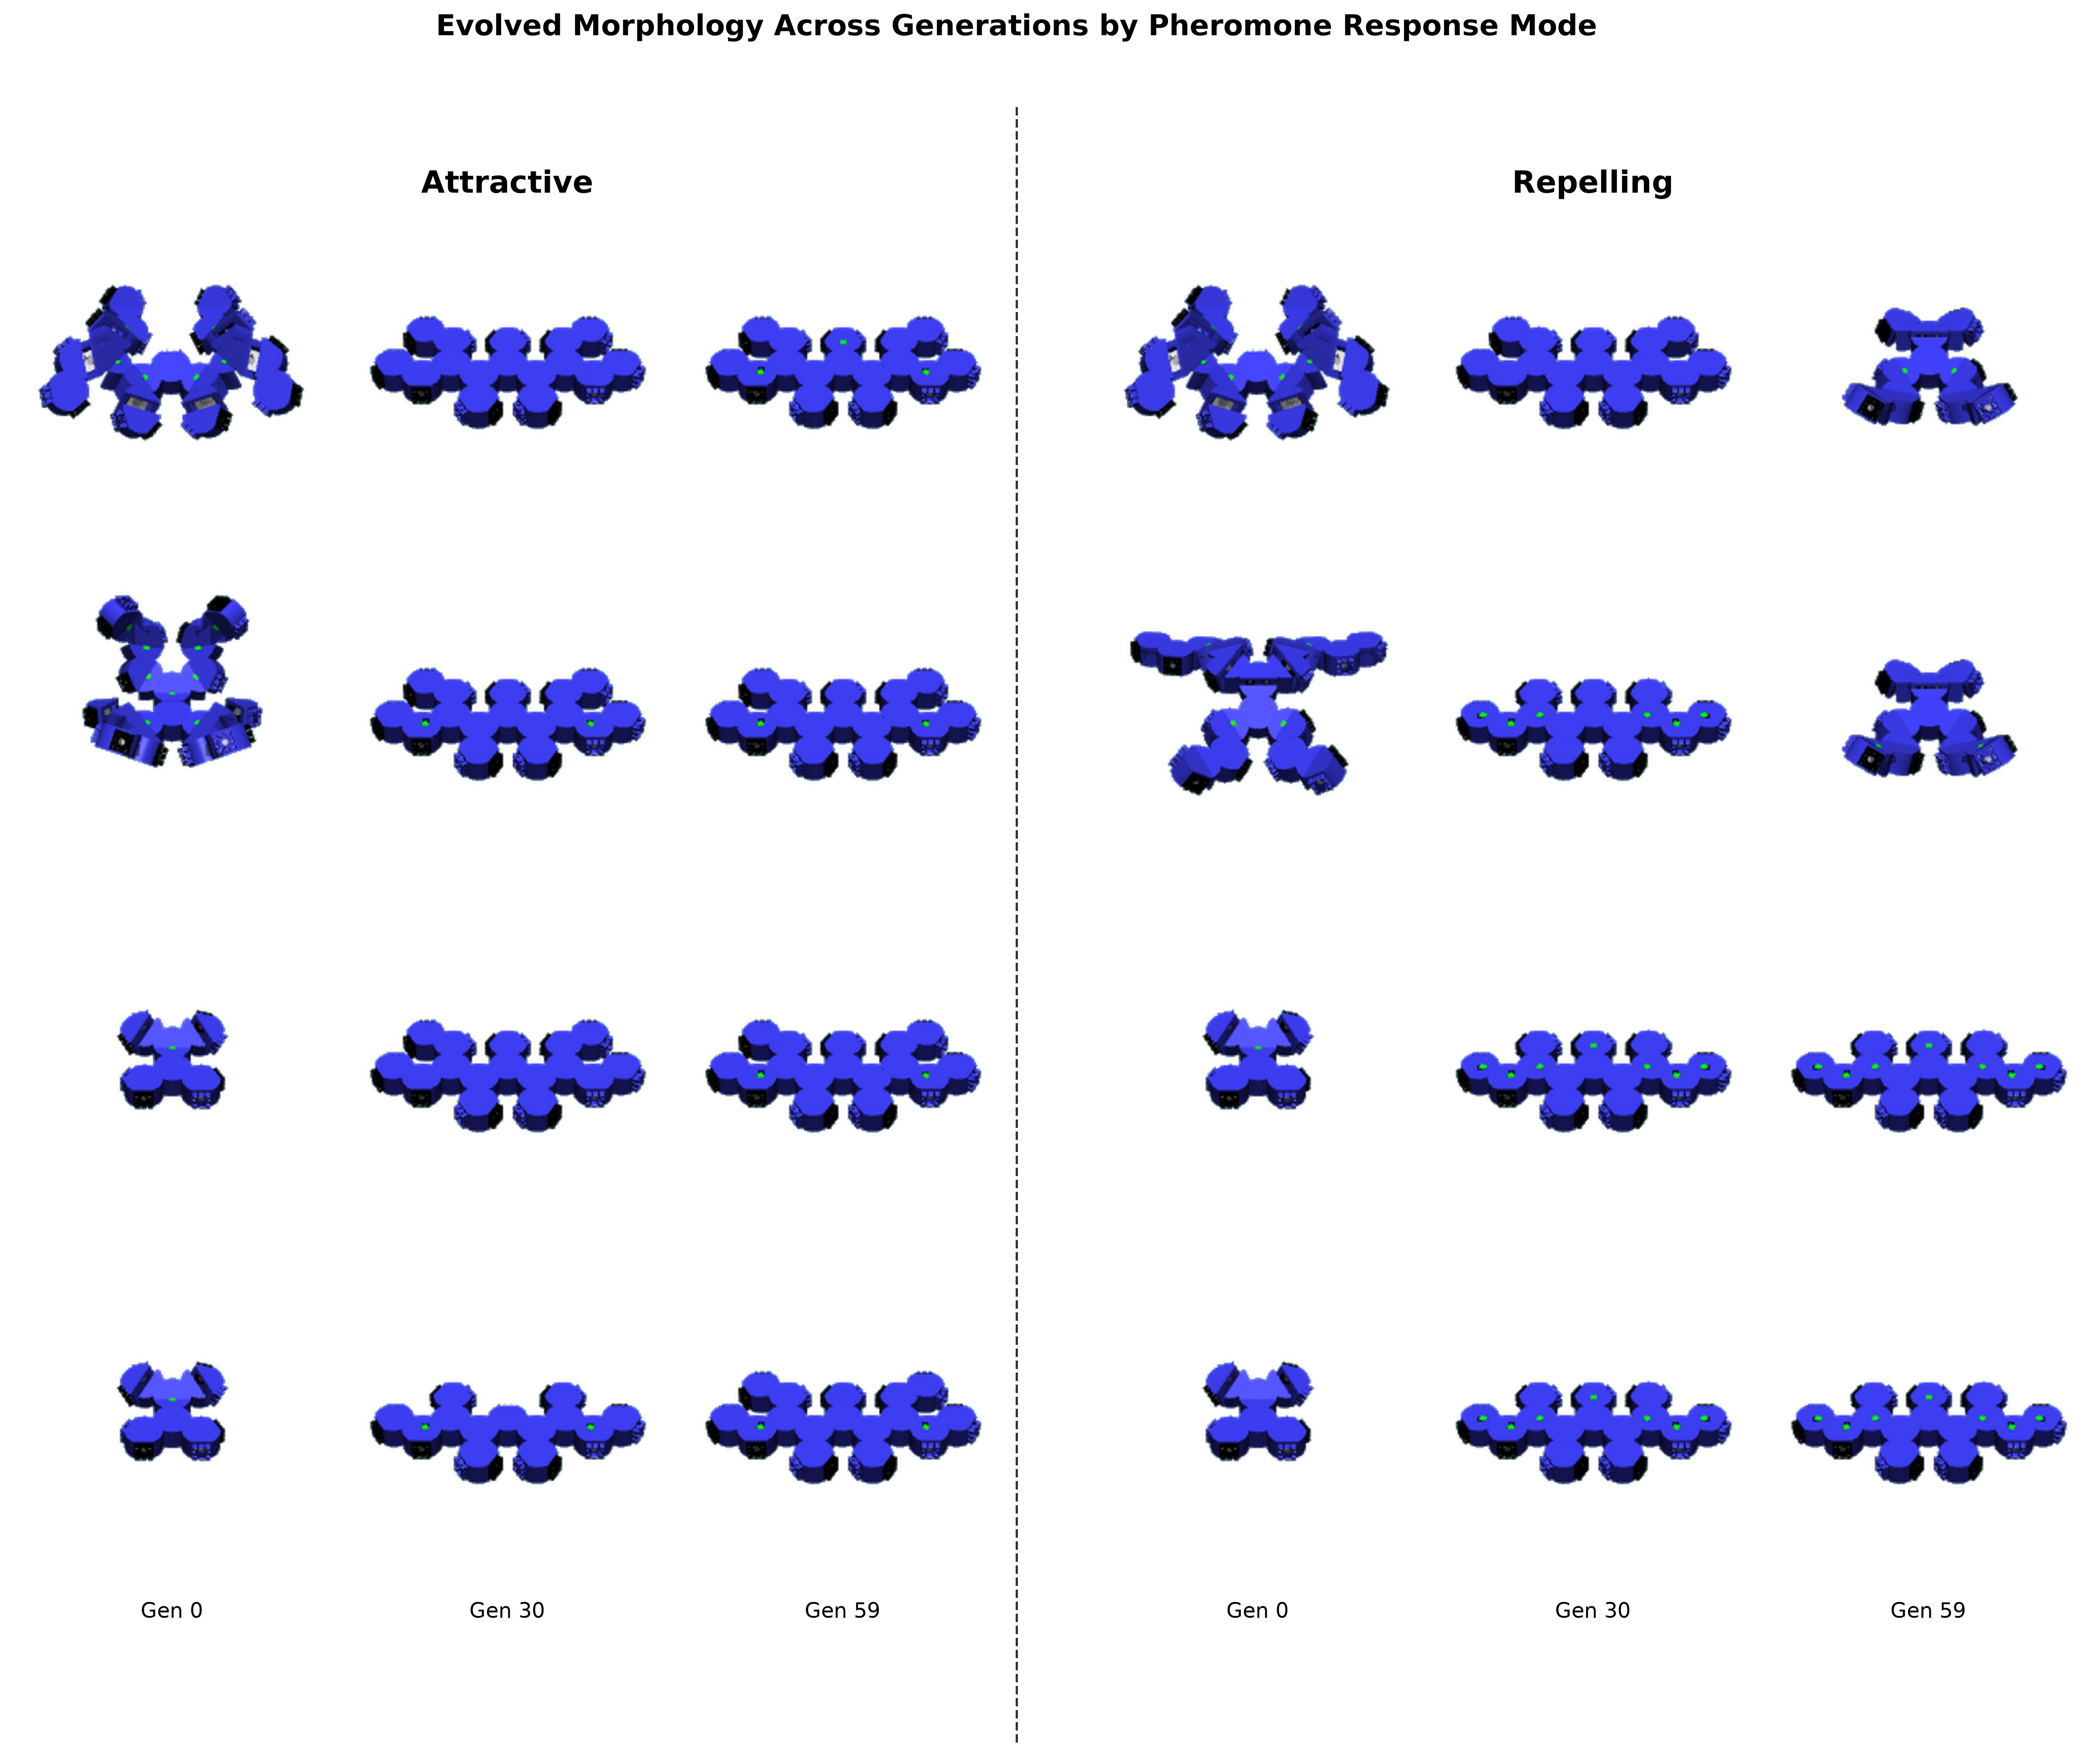
\includegraphics[width=1.0\textwidth]{morphology_grid.png}
    \caption{Representative evolved morphologies across generations, attractive versus repulsive configuration, rendered at a fixed shared scale for direct size comparison.}
    \label{fig:morphology-grid}
\end{figure}
\begin{figure}[H]
    \centering
    \begin{subfigure}[b]{0.47\linewidth}
        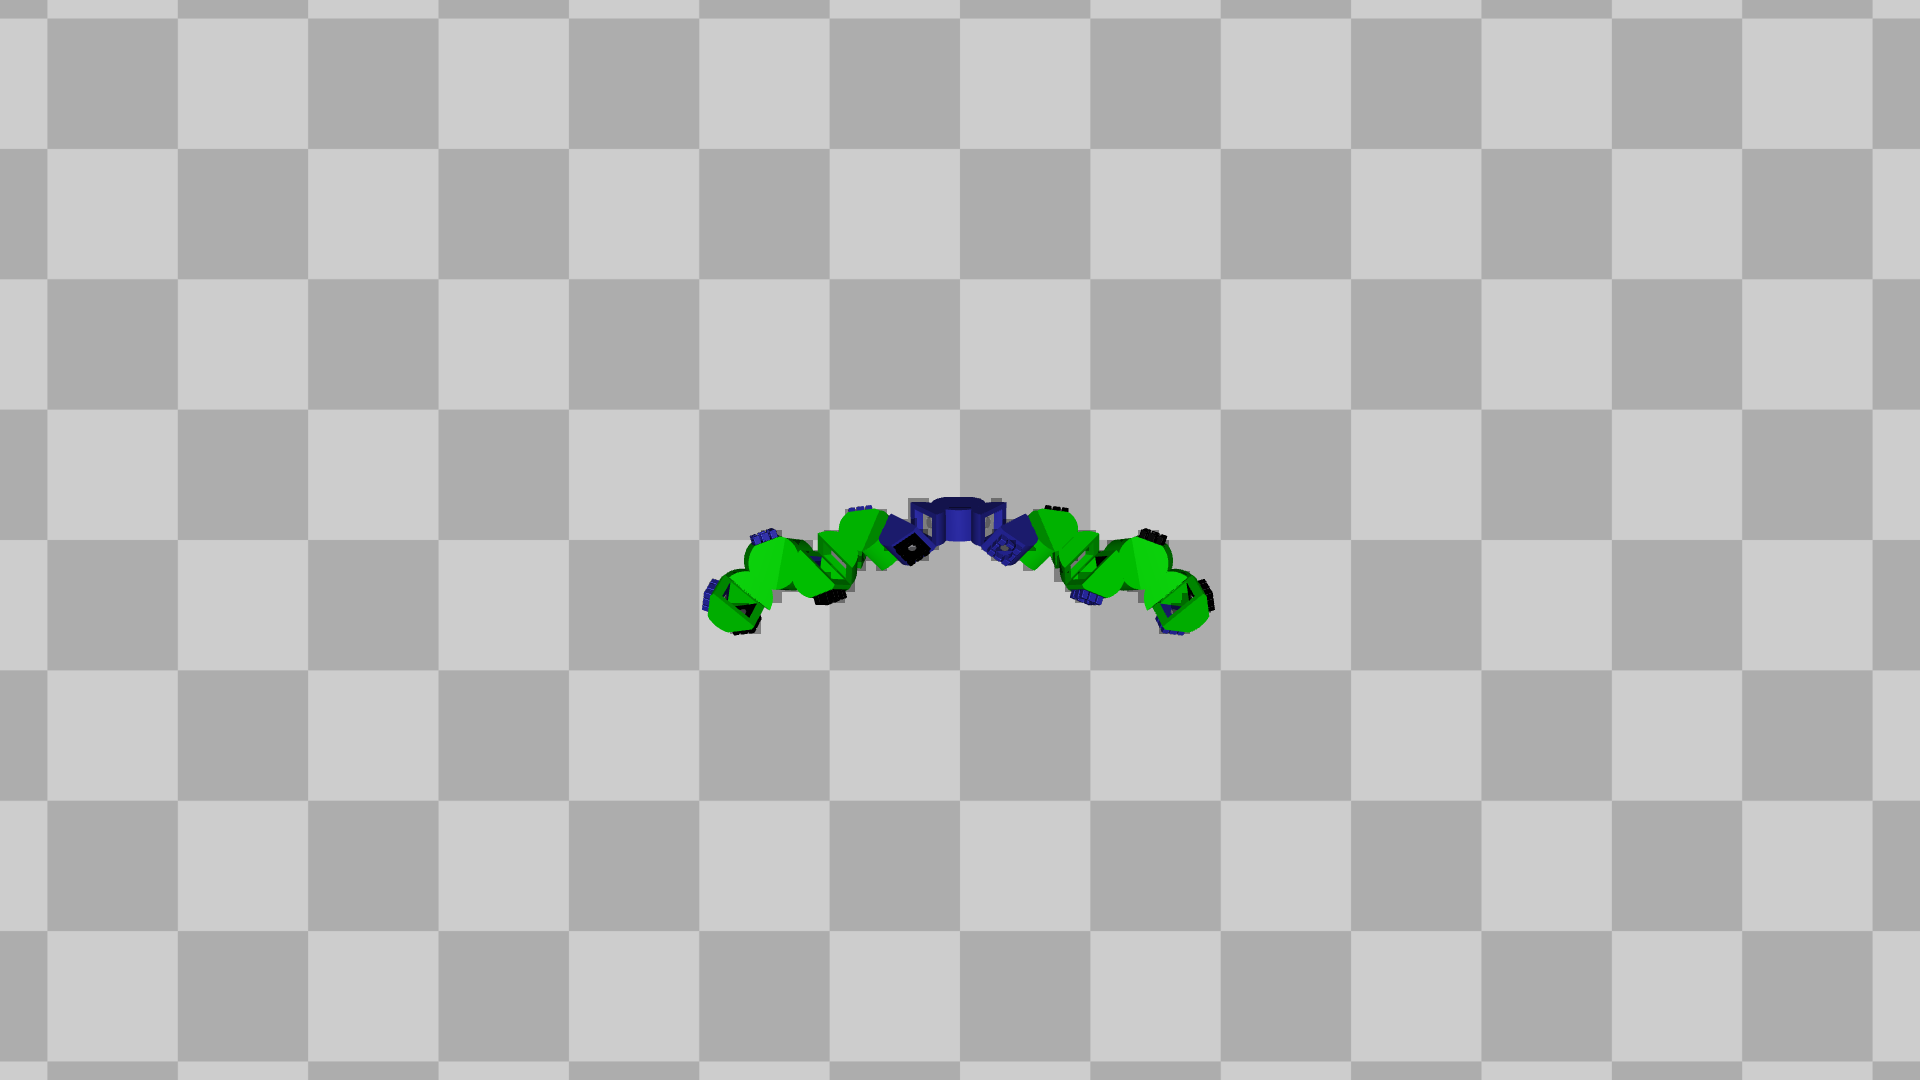
\includegraphics[width=\linewidth]{Evolved_morphology_phermone_attractive.png}
        \caption{Attractive: morphology}
        \label{fig:morph-attractive}
    \end{subfigure}
    \hfill
    \begin{subfigure}[b]{0.47\linewidth}
        \includegraphics[width=\linewidth]{Phermone_attracting_with_phermone.png}
        \caption{Attractive: yaw response}
        \label{fig:morph-attractive-yaw-response}
    \end{subfigure}
    \par\vspace{0.6em}
    \begin{subfigure}[b]{0.47\linewidth}
        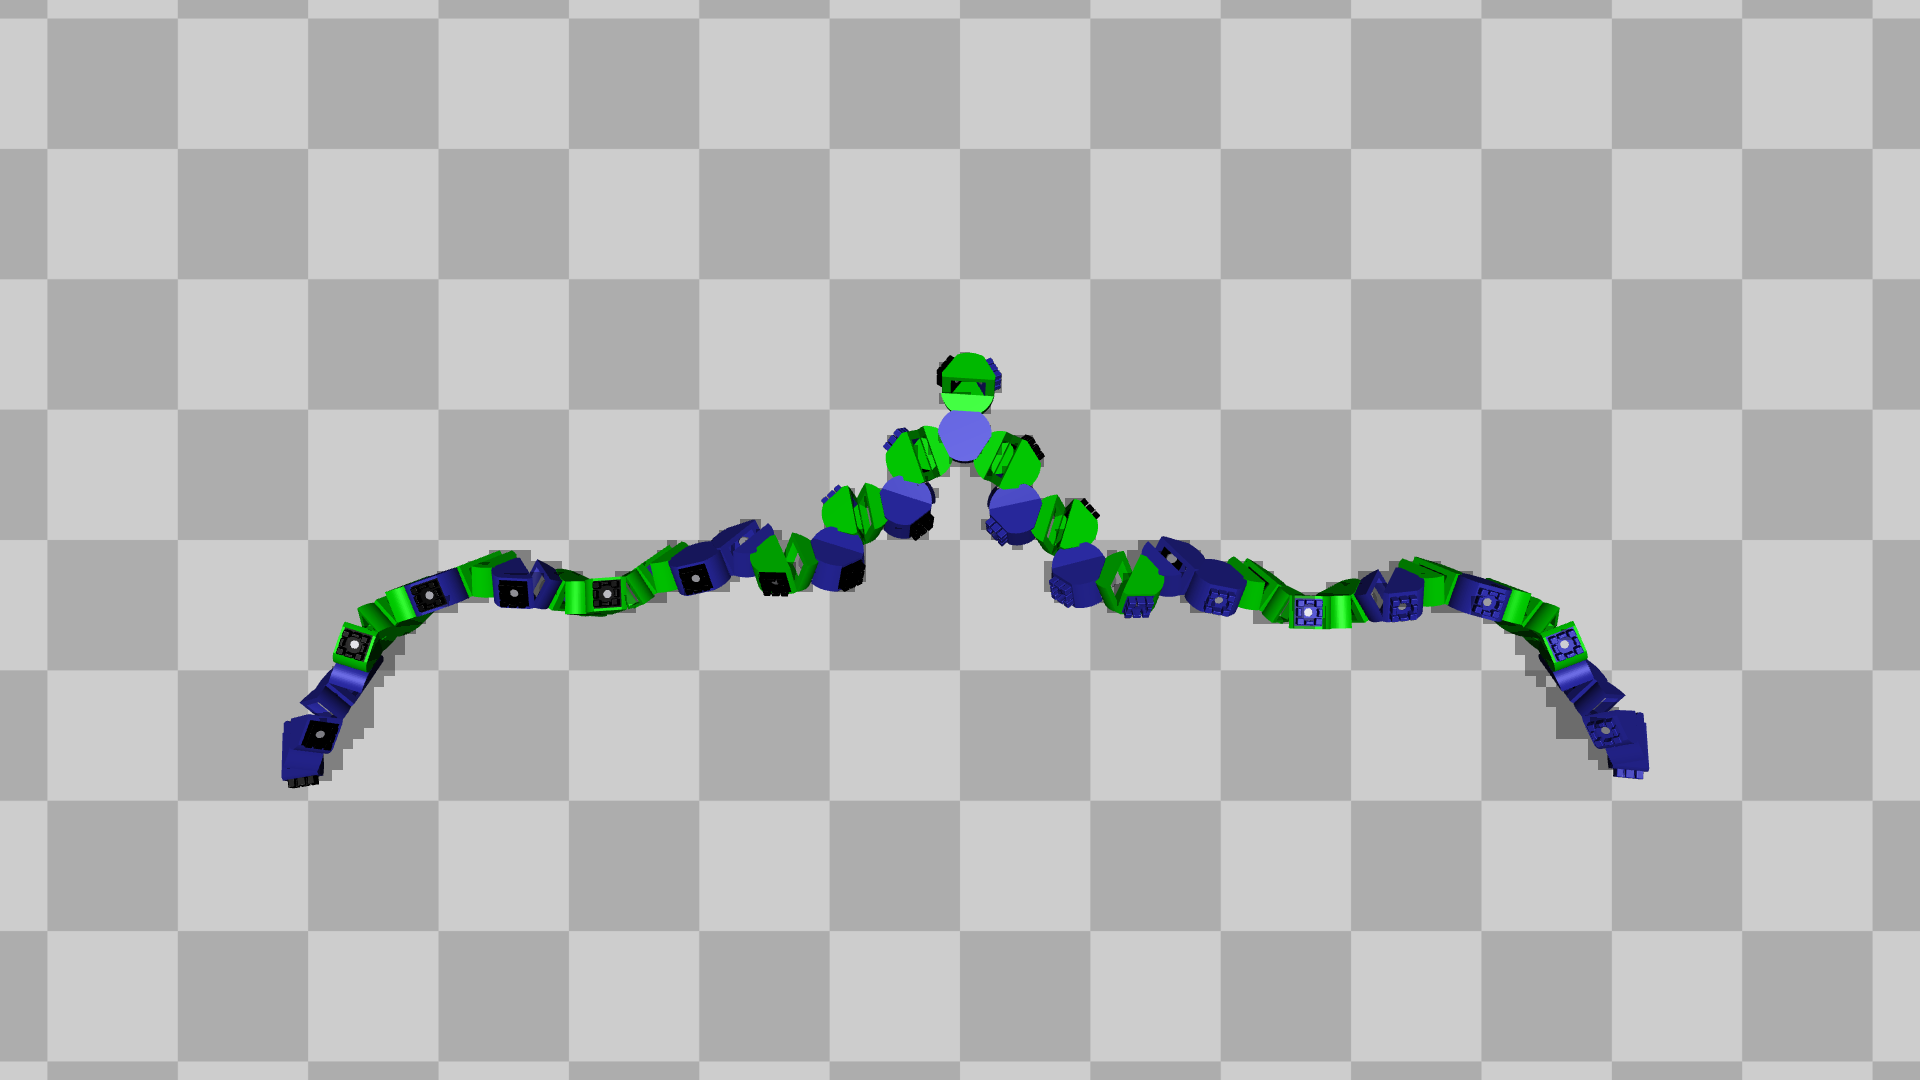
\includegraphics[width=\linewidth]{Evolved_morphology_phermone_repulsive.png}
        \caption{Repulsive: morphology}
        \label{fig:morph-repulsive}
    \end{subfigure}
    \hfill
    \begin{subfigure}[b]{0.47\linewidth}
        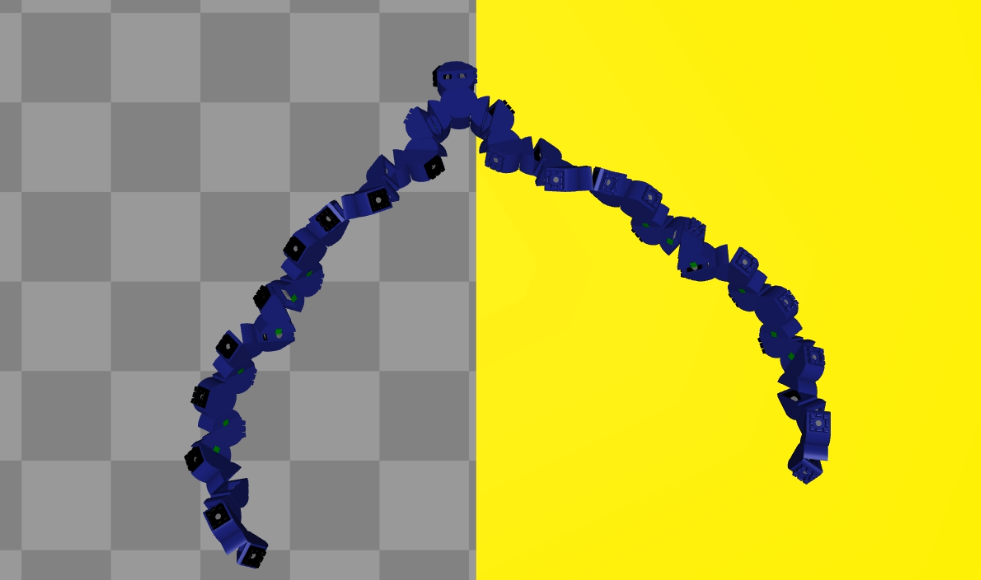
\includegraphics[width=\linewidth]{Phermone_repelling_with_phermone.png}
        \caption{Repulsive: yaw response}
        \label{fig:morph-repulsive-yaw-response}
    \end{subfigure}
    \caption{Evolved morphology and its yaw response to a left-stimulus light, attractive (top) versus repulsive (bottom) configuration. Modules that change their pheromone-sensing hinge angle are rendered in green, while modules without pheromone sensing are rendered in blue.}
    \label{fig:evolved-morphologies-both}
\end{figure}

As shown in Fig.~\ref{fig:morphology-grid}, which tracks four individual lineages from generation 0 to generation 299 in each configuration, all four tracked lineages in the repulsive configuration become visibly elongated by generation 150 and remain so at generation 299, forming curved, single-chain "worm" or "thread-like" morphologies rather than the more compact, radially branched starting shapes. In the attractive configuration this elongation is less consistent: two of the four tracked lineages flatten into a similar wavy chain by generation 299, while the other two remain closer to a compact, cross-like arrangement of short branches around the root module. This asymmetry suggests that elongation is more strongly, though not exclusively, favoured under the repulsive objective configuration than the attractive one, within the small number of lineages tracked here.

\begin{table}[htbp]
\centering
\footnotesize
\caption{Design-variable selections and objective values of the evolved individual selected by \texttt{helper\_scripts/report\_best\_last\_generation.py} in each pheromone-response configuration -- the run shown in Fig.~\ref{fig:evolved-morphologies-both} (\texttt{output/evolution\_run}, generation 299, rank 25, individual \texttt{ind10}; \texttt{output/evolution\_run\_repulsive}, generation 299, rank 12, individual \texttt{ind17}). }
\label{tab:evolved-morphology-values}
\begin{tabular}{@{}lp{3.6cm}p{3.6cm}@{}}
\toprule
& \textbf{Attractive} & \textbf{Repulsive} \\
\midrule
\multicolumn{3}{@{}l}{\textit{Design variables}} \\
\addlinespace[2pt]
Module count (post-mirror) & 13 & 38 \\
Fold-type distribution (rigid / mountain / valley) & 1 / 12 / 0 & 5 / 23 / 10 \\
Hinge angle $\theta$ & $7.66^{\circ}$ & $31.09^{\circ}$ \\
Light-sensitive nodes & 8 & 19 \\
Light-detection hinge angle $\theta_{light}$ & $43.51^{\circ}$ & $20.85^{\circ}$ \\
\addlinespace[4pt]
\multicolumn{3}{@{}l}{\textit{Objective values}} \\
\addlinespace[2pt]
Scalarised fitness & $0.303079$ & $0.514673$ \\
$f_1$ -- Folded-gait velocity & $0.0311$ m/s & $0.0292$ m/s \\
$f_2$ -- Entropy gain $\Delta H = \tilde H_{3D}-\tilde H_{2D}$ & $-0.0029$ & $0.2307$ \\
$f_3$ -- Pheromone yaw response & $179.3^{\circ}$ & $-105.1^{\circ}$ \\
$f_4$ -- Pheromone speed response & $21.649$ & $0.440$ \\
\bottomrule
\end{tabular}
\end{table}

The morphology figures provide end-to-end evidence for O-1 to O-3: graph designs were generated, converted into assemblies, folded and evaluated in the physics simulator. They also show how AO-1 was changed from surrogate fitness prediction to light-response objectives. As shown in Fig.~\ref{fig:evolved-morphologies-both}, both rendered individuals are bilaterally symmetric, as expected from the mirror construction (Section~\ref{sec:symmetry}), and their light-sensitive modules are rendered in green against blue non-light-sensitive modules -- consistent with the 8-of-13 and 19-of-38 light-sensitive node counts reported in Table~\ref{tab:evolved-morphology-values}. The attractive individual is a compact, arch-shaped assembly, while the repulsive individual is a long, curved single chain roughly three times its module count, matching the general elongation pattern in Fig.~\ref{fig:morphology-grid} discussed above for this specific pair of selected individuals. The two response modes should therefore be read as separate design problems, not as proof that one morphology can optimise both behaviours at once.

\section{RL-Assisted NSGA-III versus Standard NSGA-III Comparison}
\label{sec:rl-vs-random}
\begin{figure}[H]
    \centering
    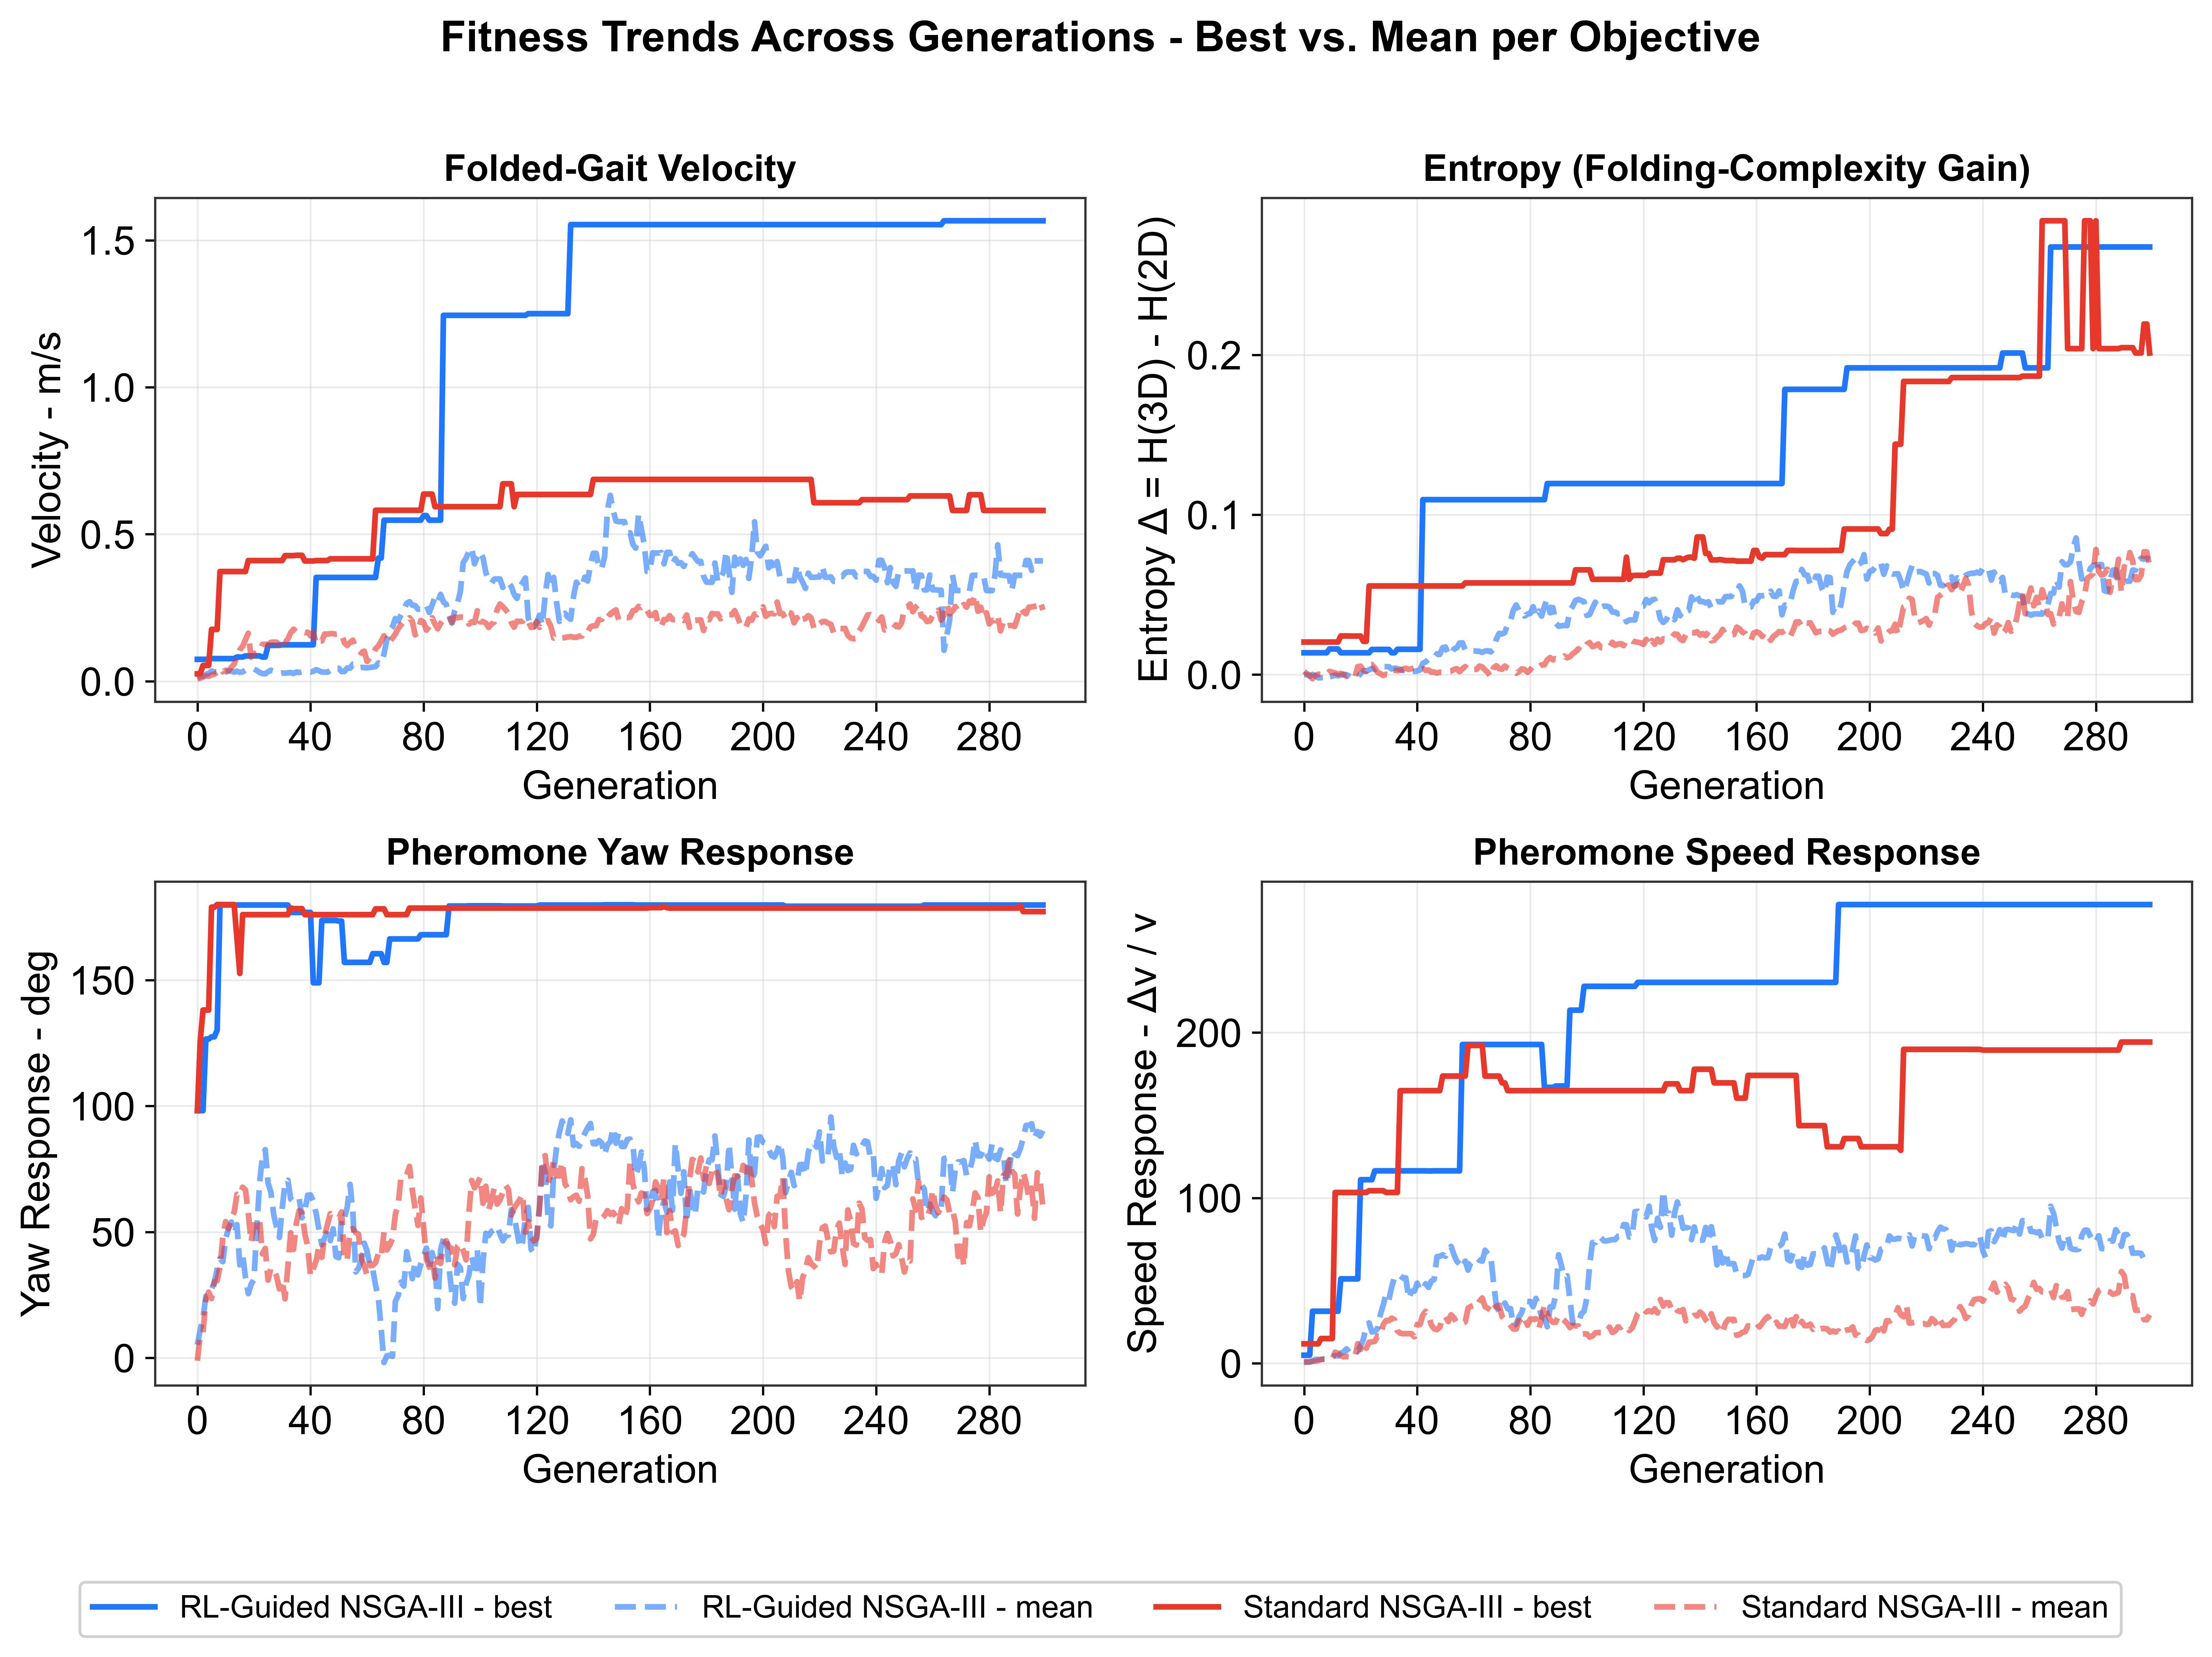
\includegraphics[width=0.85\linewidth]{fitness_trends_comparison.png}
    \caption{Best and mean scalarized fitness per objective, RL-assisted versus standard breeding, over a 300-generation comparison run.}
    \label{fig:fitness-trends-comparison}
\end{figure}
\begin{figure}[H]
    \centering
    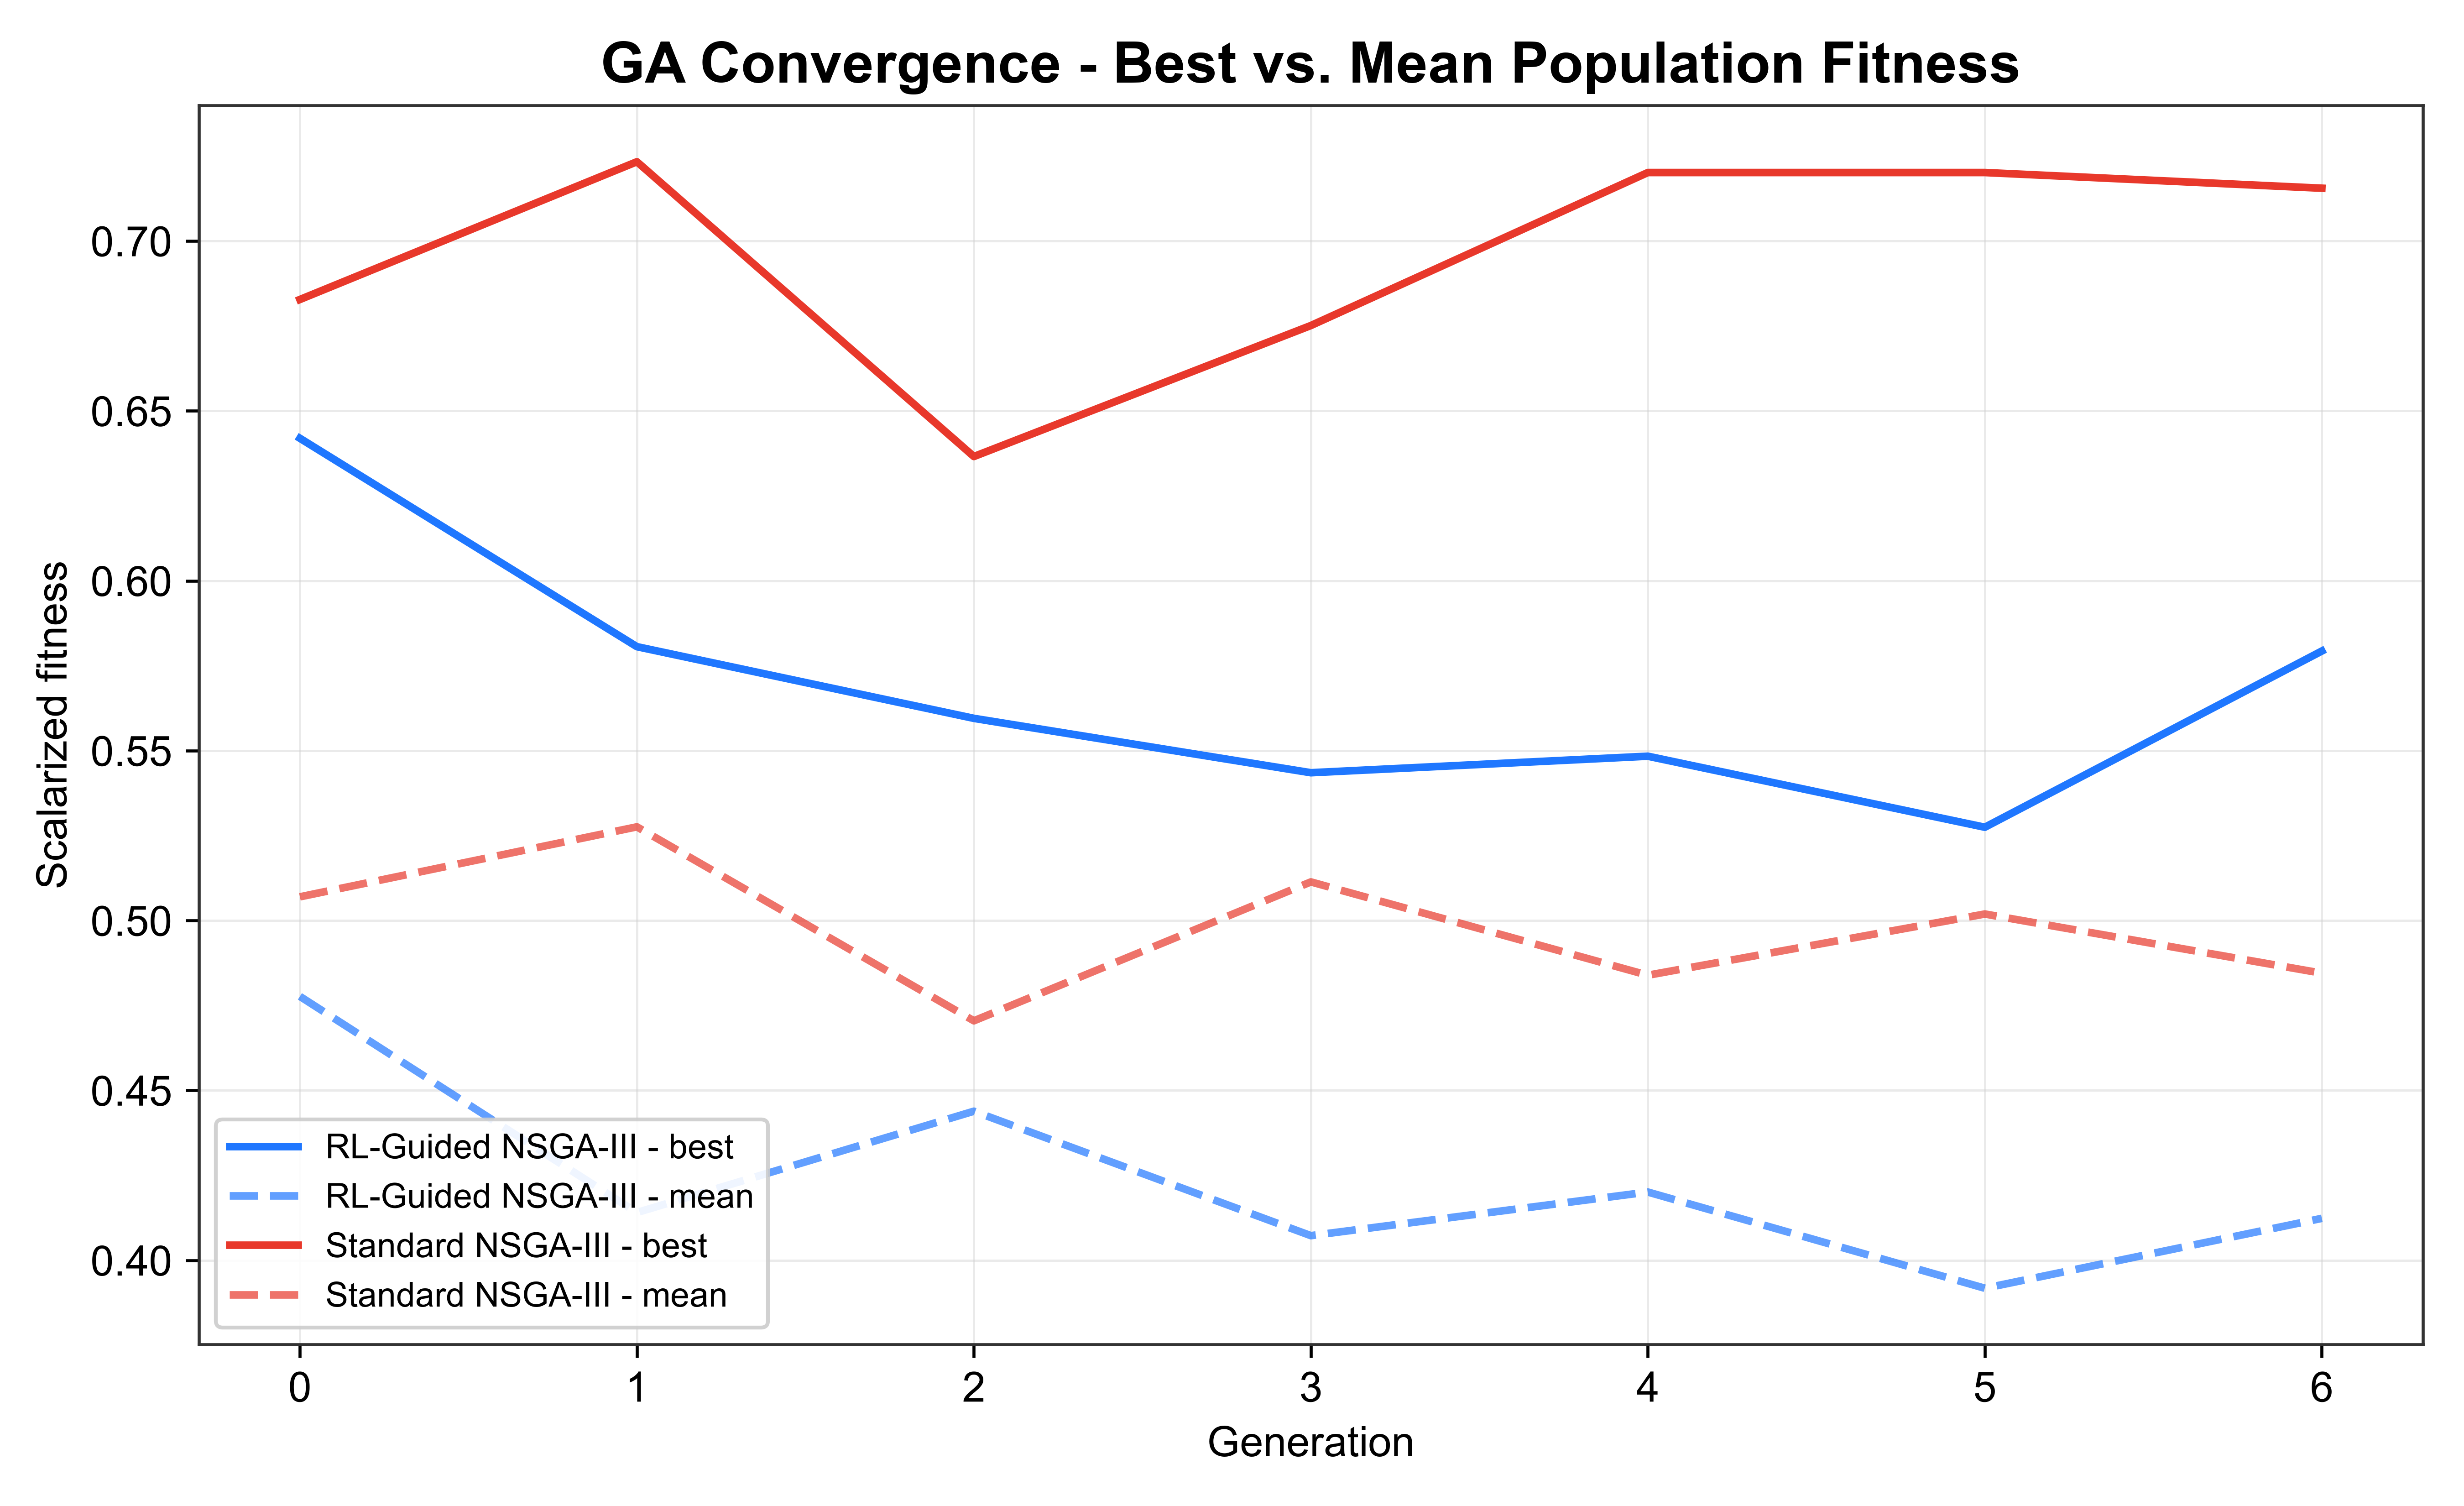
\includegraphics[width=0.85\linewidth]{convergence_comparison.png}
    \caption{GA convergence: best and mean scalarized population fitness across generations, RL-assisted versus standard breeding.}
    \label{fig:convergence-comparison}
\end{figure}

\begin{figure}[H]
    \centering
    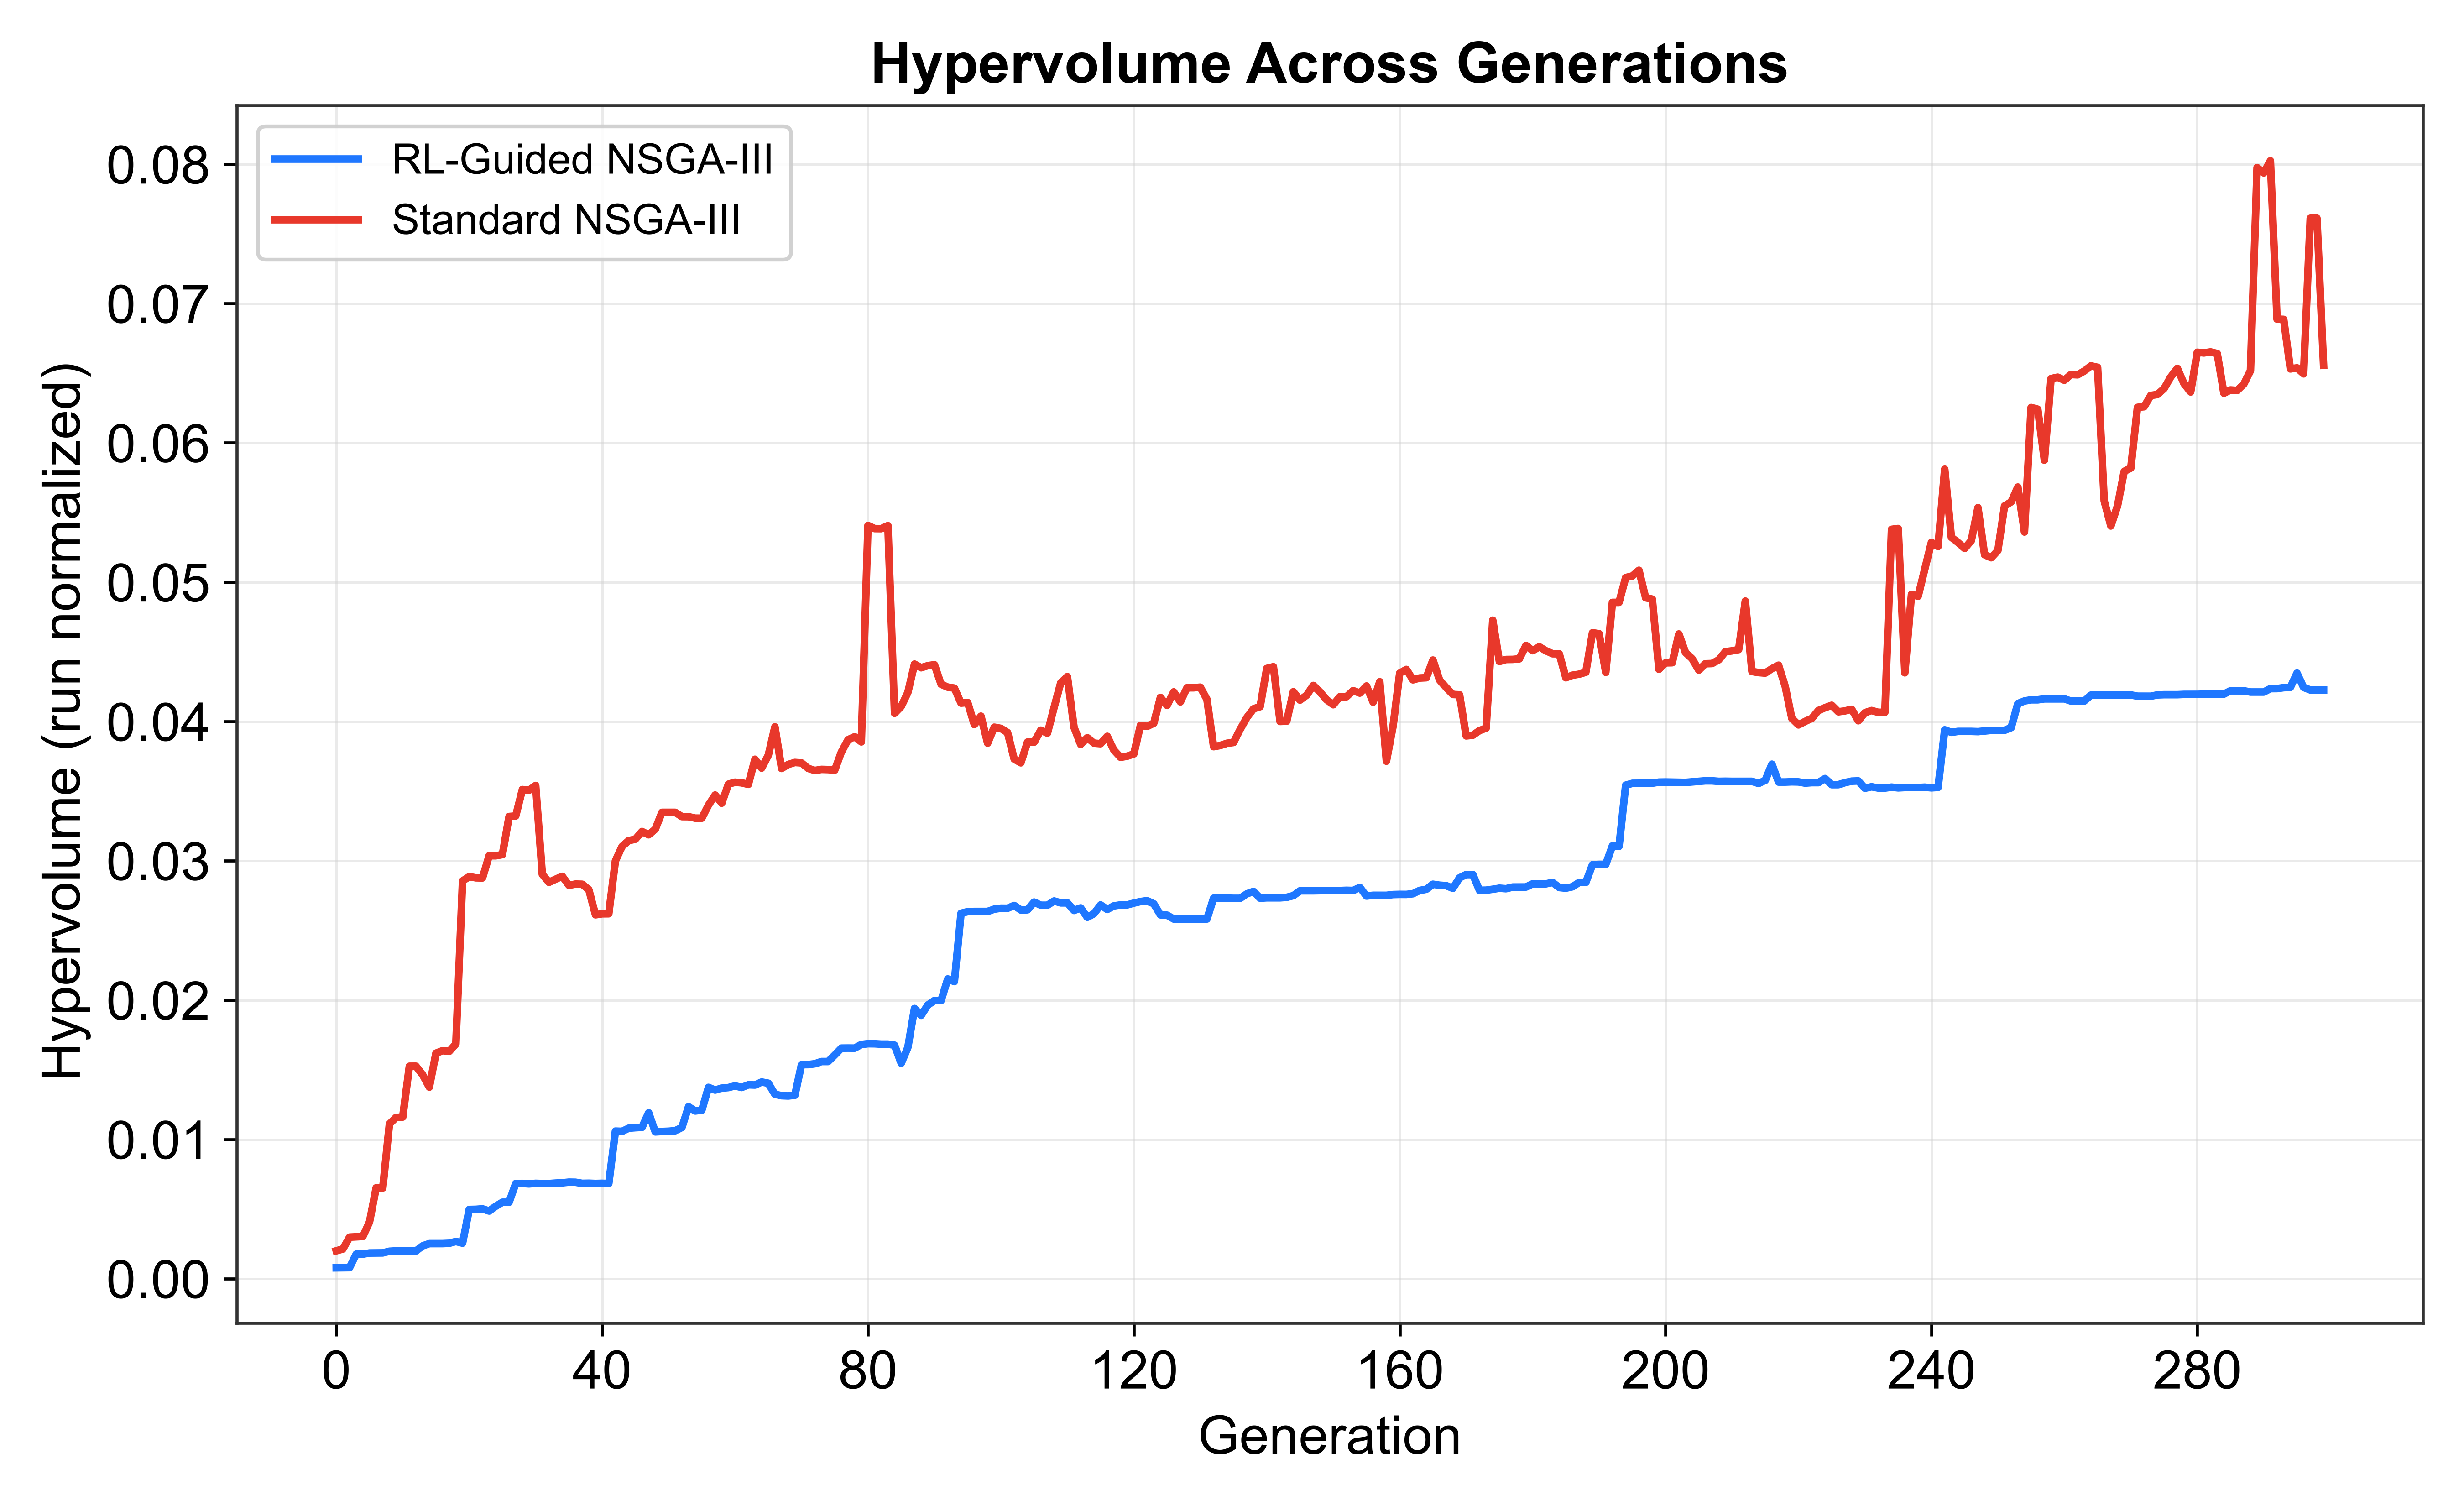
\includegraphics[width=0.85\linewidth]{hypervolume_comparison.png}
    \caption{Hypervolume comparison, RL-assisted versus standard breeding, over the same comparison run.}
    \label{fig:hypervolume-comparison}
\end{figure}
\begin{figure}[H]
    \centering
    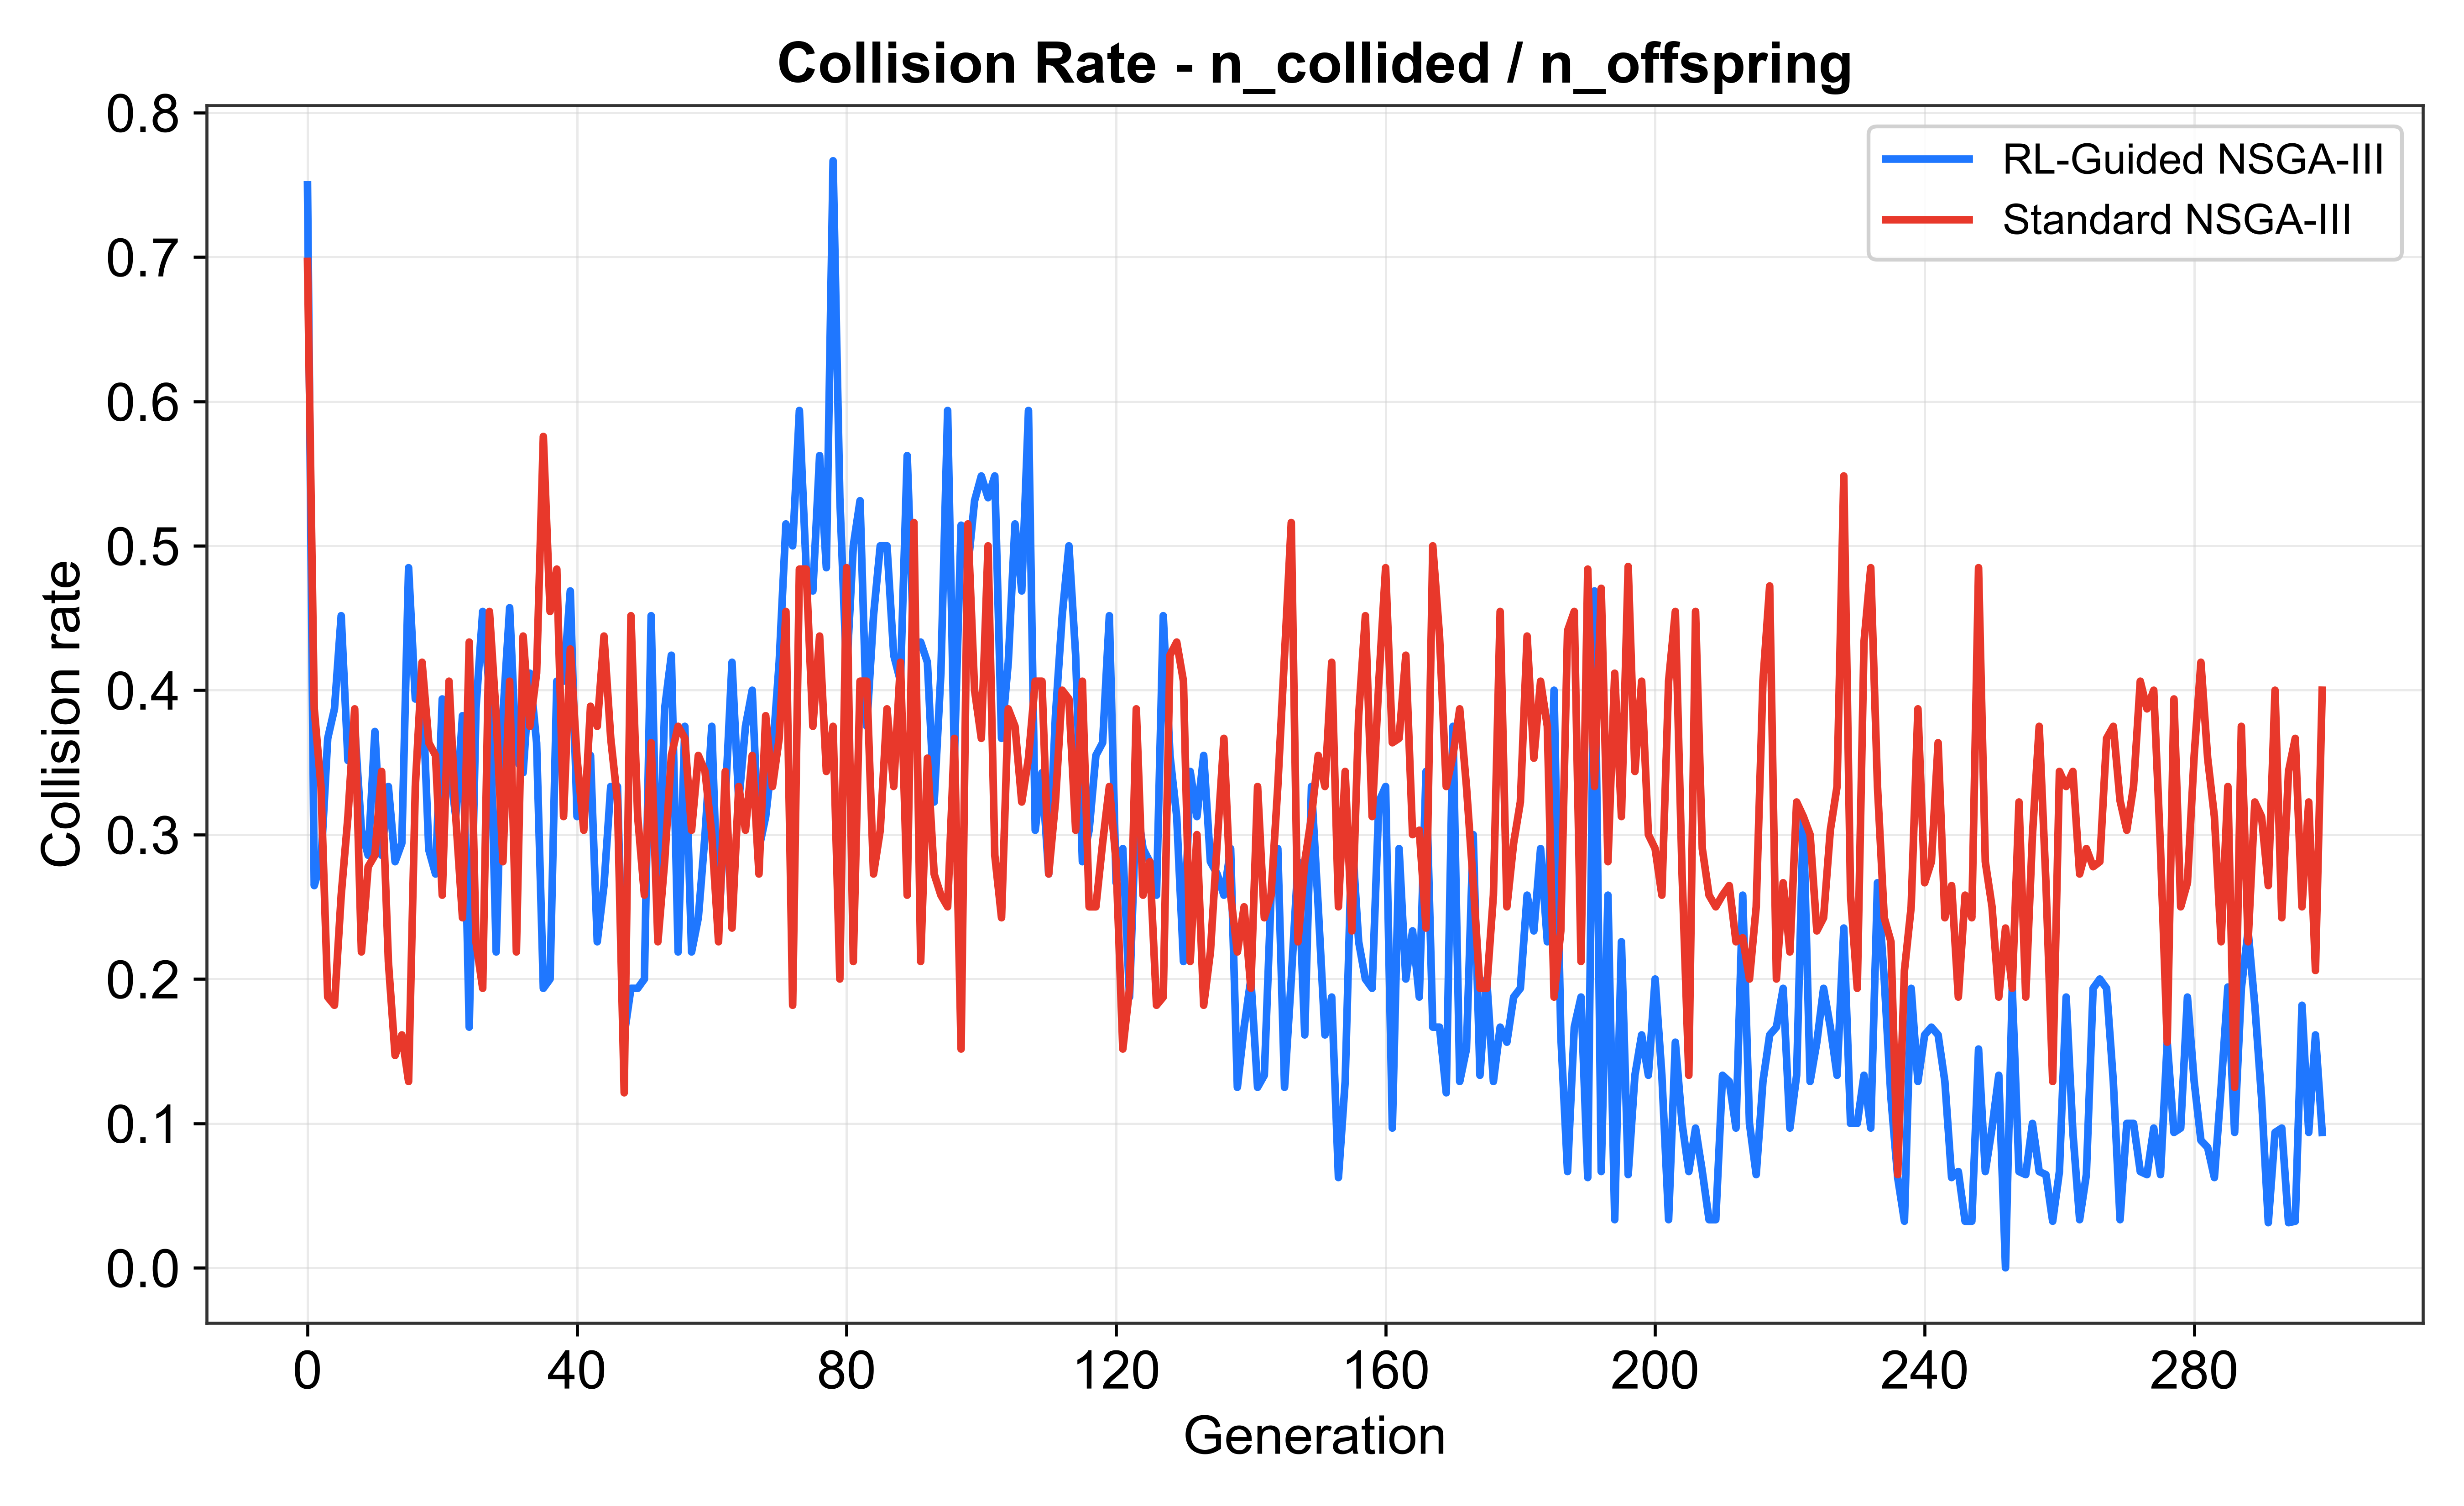
\includegraphics[width=0.85\linewidth]{collision_rate_comparison.png}
    \caption{Collision rate ($n_{\mathrm{collided}}/n_{\mathrm{offspring}}$), RL-assisted versus standard breeding, over the same comparison run.}
    \label{fig:collision-rate-comparison}
\end{figure}

\begin{figure}[H]
    \centering
    \begin{subfigure}[b]{\linewidth}
        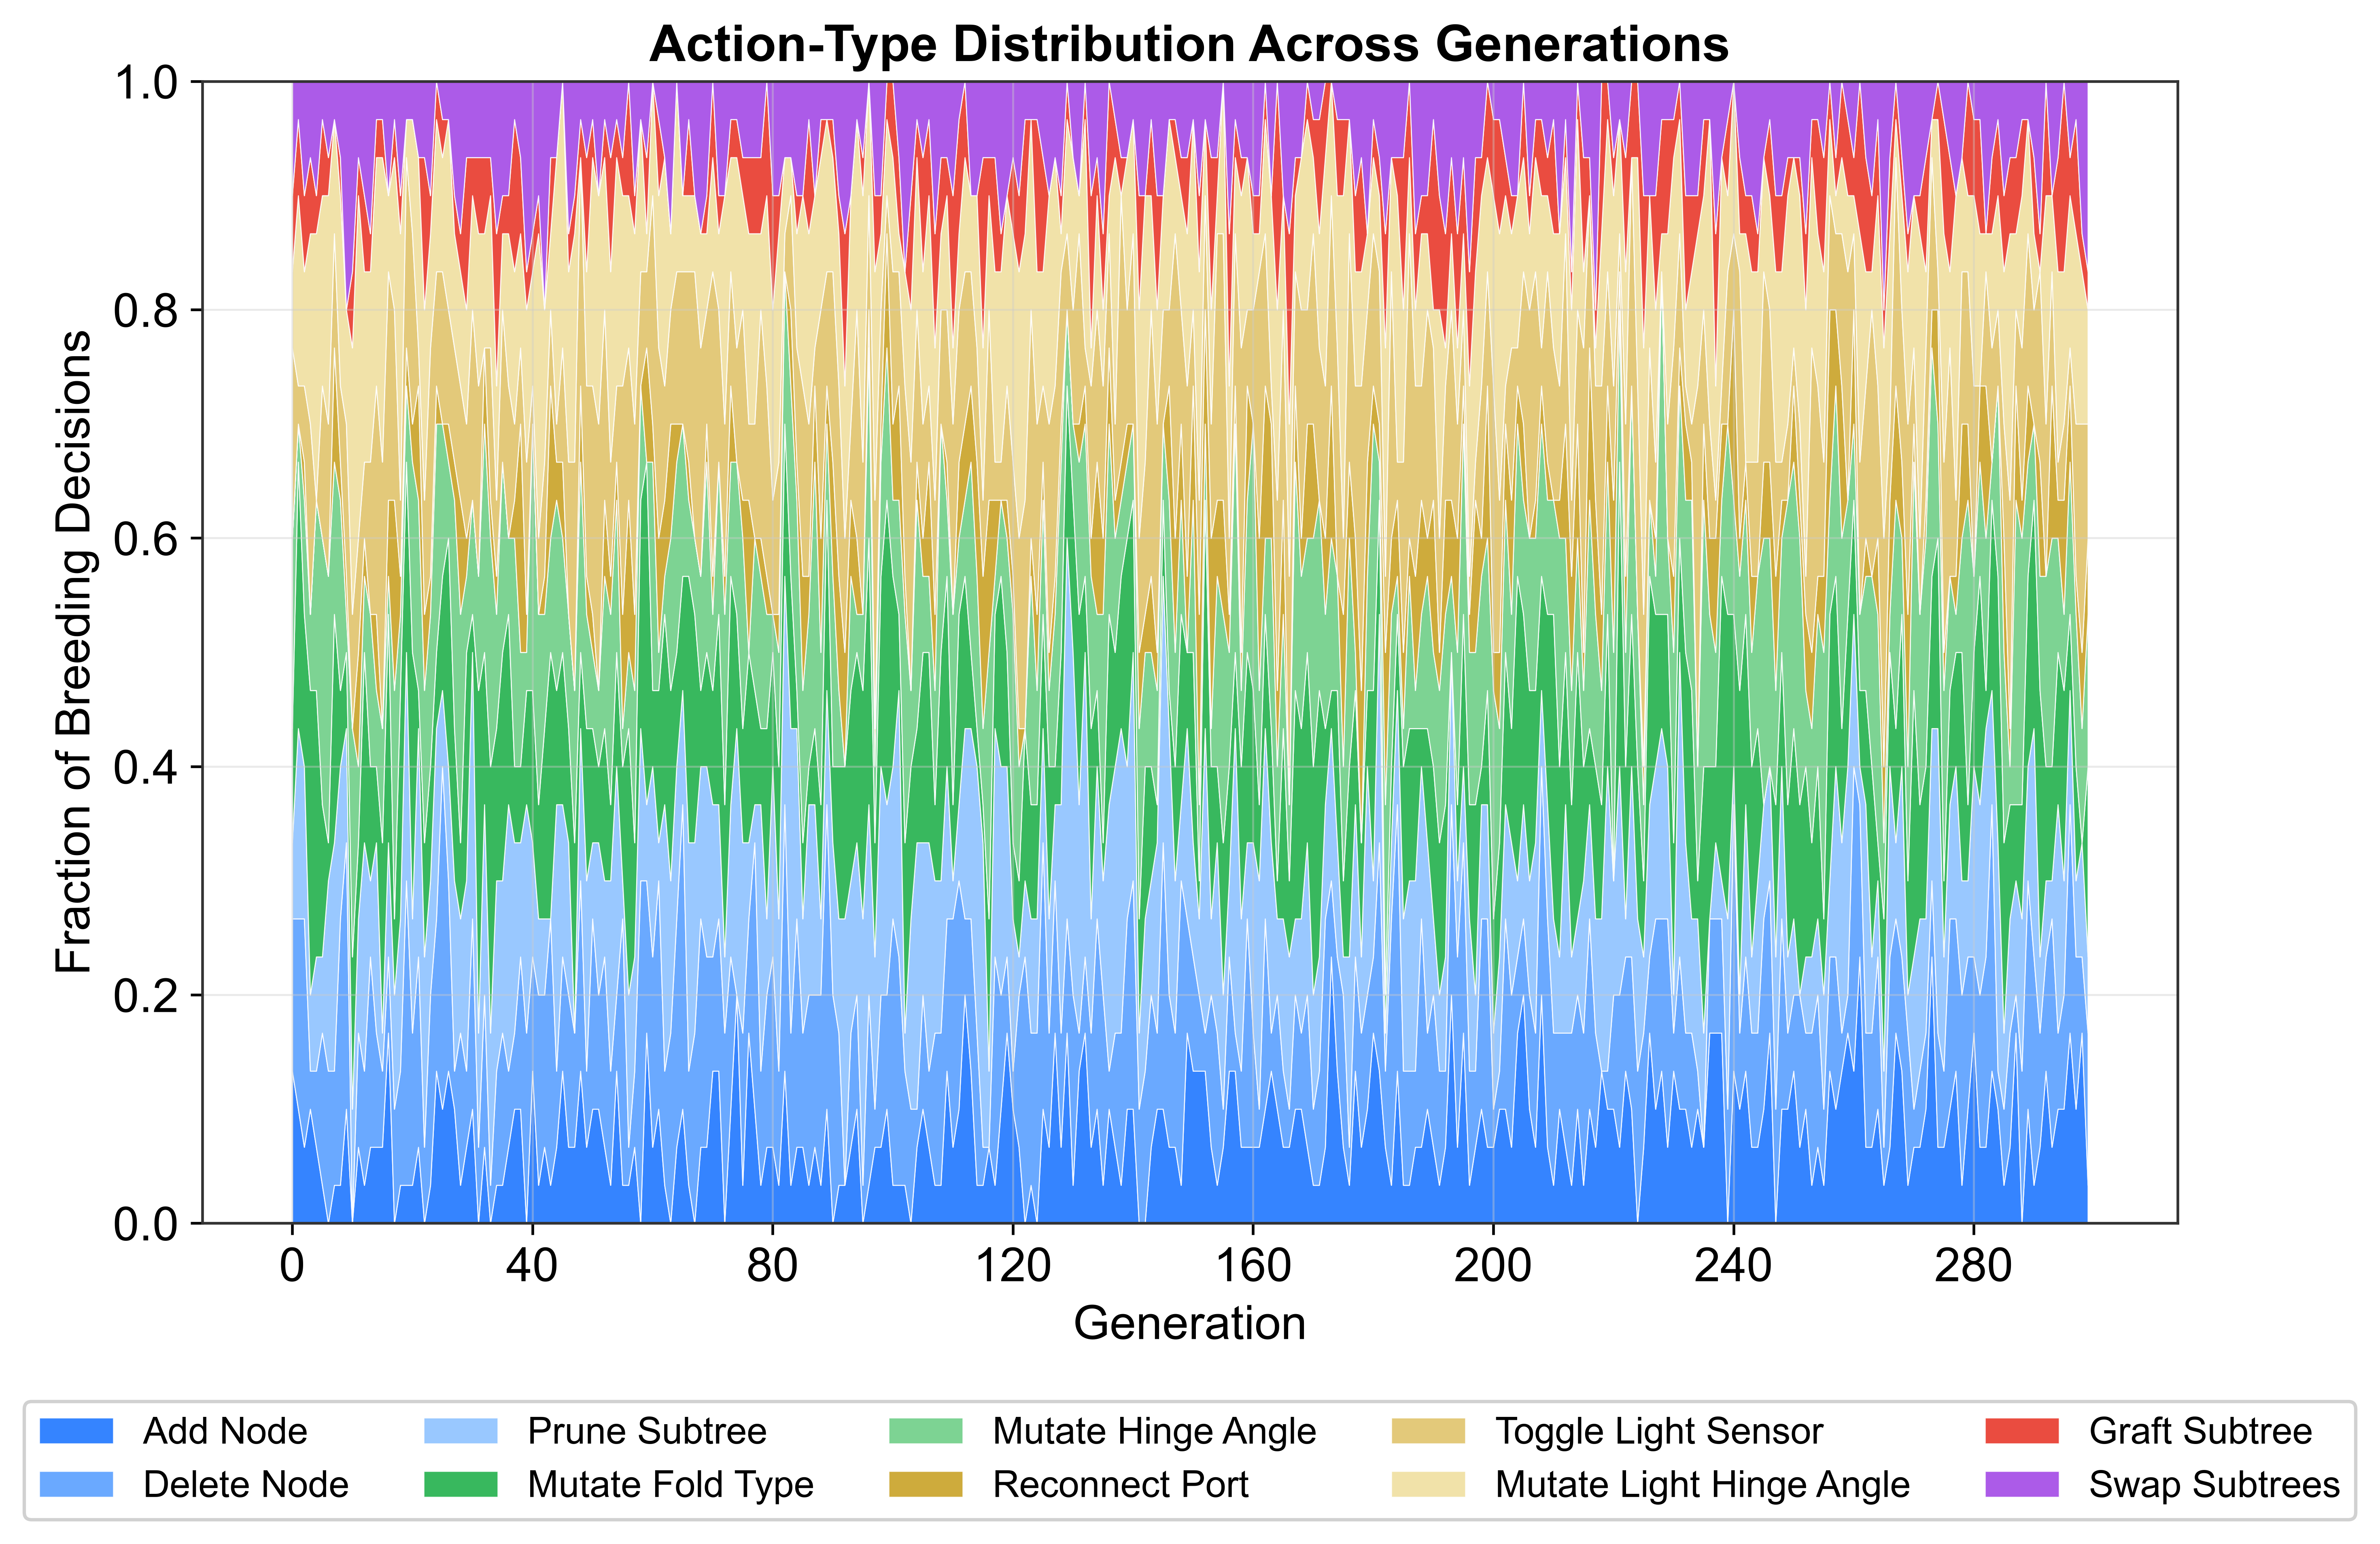
\includegraphics[width=\linewidth]{norl_action_distribution.png}
        \caption{Standard (uniform-random) breeding arm.}
        \label{fig:norl-action-distribution}
    \end{subfigure}
    \par\vspace{0.6em}
    \begin{subfigure}[b]{\linewidth}
        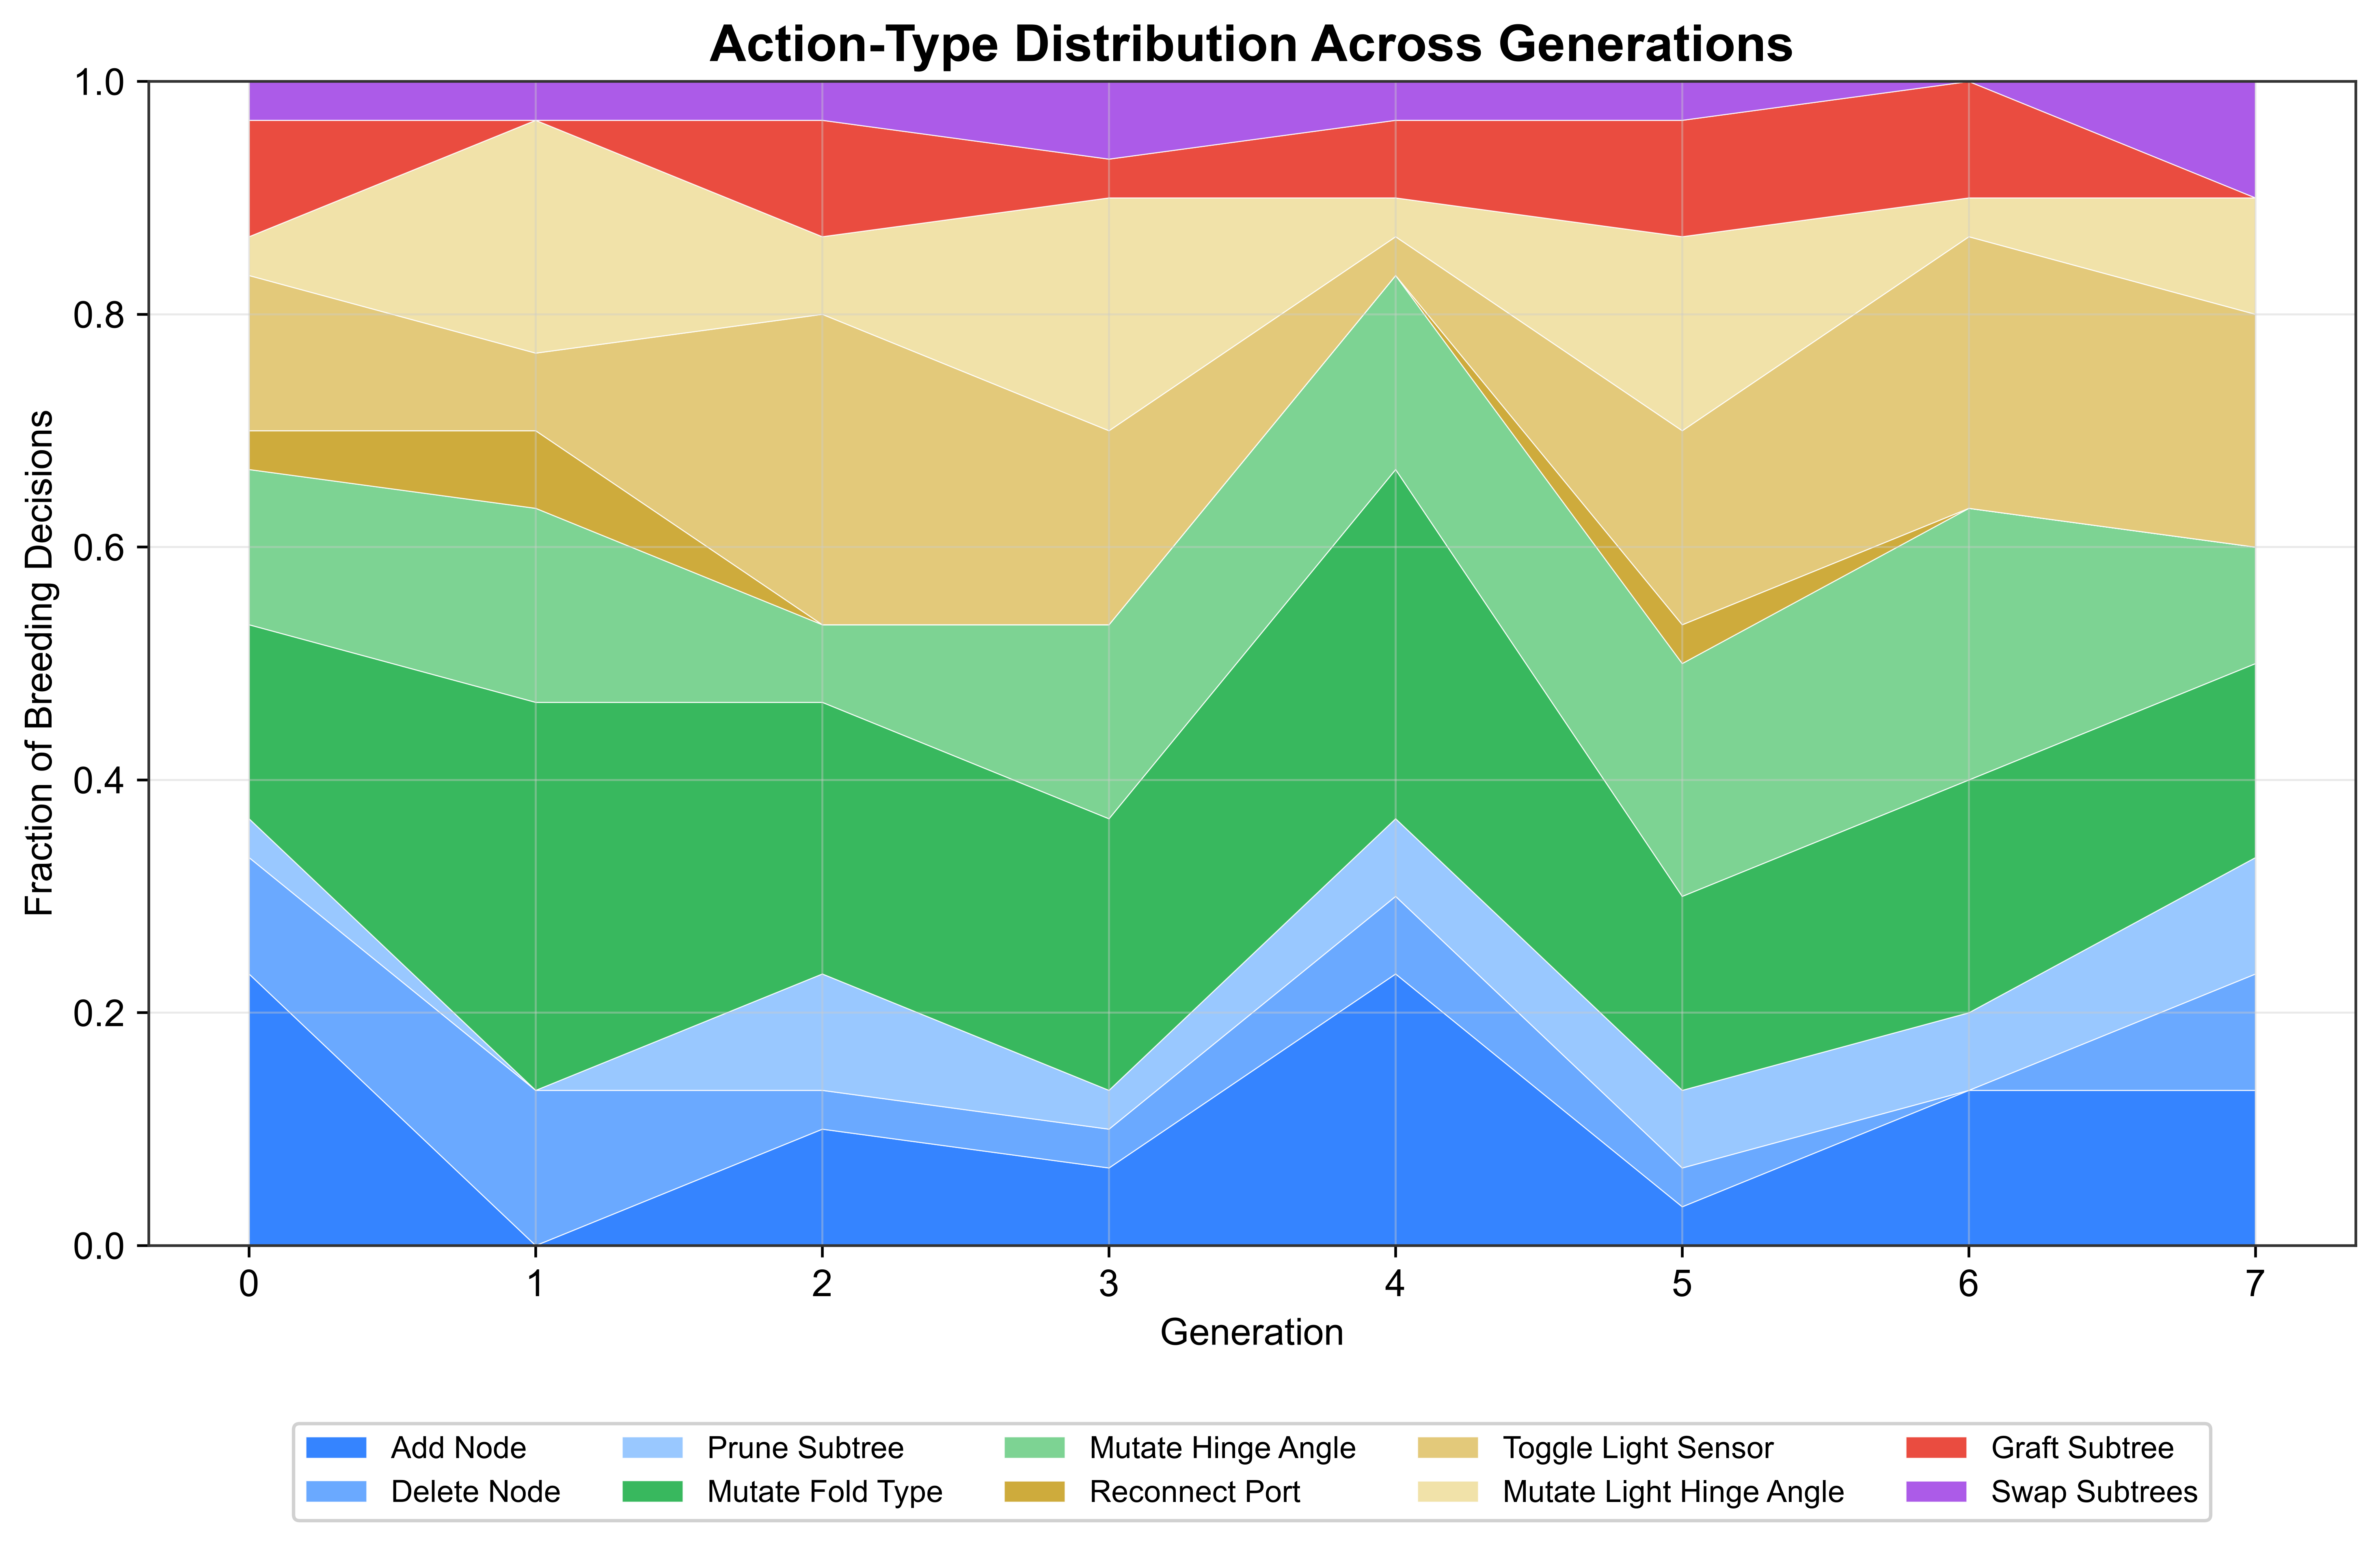
\includegraphics[width=\linewidth]{action_distribution.png}
        \caption{RL-assisted arm.}
        \label{fig:action-distribution}
    \end{subfigure}
    \caption{Fraction of breeding decisions by grammar action type per generation, standard versus RL-assisted breeding.}
    \label{fig:action-distribution-both}
\end{figure}

The four metrics shown do not agree on a single winner at this scale, and are reported here as measured rather than resolved into one verdict. On per-objective best fitness (Fig.~\ref{fig:fitness-trends-comparison}), the RL-assisted arm reaches a clearly higher best folded-gait velocity (approximately 1.57 vs.\ 0.57\,m/s by the run's end) and a higher best speed response (approximately 280 vs.\ 190) than the standard arm; the two arms reach a similar best yaw response, both saturating near the $179$-$180^\circ$ ceiling by around generation 90; and best entropy gain is broadly comparable between the arms for most of the run, with the standard arm briefly ahead in the final generations. On scalarised best fitness (Fig.~\ref{fig:convergence-comparison}), the RL-assisted arm leads clearly for roughly the first 90 generations, the two arms interleave closely from about generation 90 to 250, and the standard arm is modestly ahead for the remainder of the run. On hypervolume (Fig.~\ref{fig:hypervolume-comparison}) -- the primary many-objective convergence measure adopted in Section~\ref{sec:evo-learning} -- the standard arm is higher than the RL-assisted arm essentially throughout the run, ending at approximately 0.065--0.08 versus approximately 0.04, indicating a larger or better-spread non-dominated front at the population level despite the RL arm's stronger individual best values on some objectives. On collision rate (Fig.~\ref{fig:collision-rate-comparison}), the two arms are similar and noisy (roughly 0.2--0.5) for about the first 130 generations, after which the RL-assisted arm's collision rate drops and stays consistently lower (mostly below 0.2) while the standard arm continues to fluctuate across its earlier range for the rest of the run.

These results are not contradictory once it is recalled what each metric measures: an RL-guided policy that concentrates variation on the specific edits that push a few objectives to strong best-individual values, while increasingly favouring lower-risk parameter mutations in later generations (Section~\ref{sec:rl-diagnostics}), can produce strong best-of-run values on some objectives without necessarily producing a larger or more diverse non-dominated population front, which is what hypervolume tracks. Read this way, the RL-assisted policy has not demonstrated an unqualified advantage over standard breeding at this scale: it wins clearly on two of four individual objectives and on collision avoidance in the second half of the run, but loses on the paper's own primary convergence measure (hypervolume) and on scalarised best fitness in the run's final third. This is a more nuanced result than either "RL is better" or "RL is worse," and a stronger conclusion in either direction would require multiple independent seeds under matched generation budgets, which is proposed as future work (Section~\ref{ch:conclusion}).

The action-distribution plots (Fig.~\ref{fig:action-distribution-both}) show that, with collision outcomes now excluded from the RL reward stream entirely (Section~\ref{sec:rl-actor-critic}), all ten grammar actions remain in active use by the RL-assisted policy throughout the full 300 generations -- there is no collapse onto one or two actions of the kind seen under the earlier, penalty-based reward design (Fig.~\ref{fig:rl-cp-action-distribution}). The two crossover actions (Graft Subtree, Swap Subtrees) are visibly a smaller, but persistent, share of decisions than the mutation actions in both arms; Section~\ref{sec:rl-diagnostics} quantifies this imbalance directly from the sample counts behind each action's reward statistics.

\section{RL Training Behaviour and Diagnostics}
\label{sec:rl-diagnostics}
\begin{figure}[H]
    \centering
    \begin{subfigure}[b]{0.48\linewidth}
        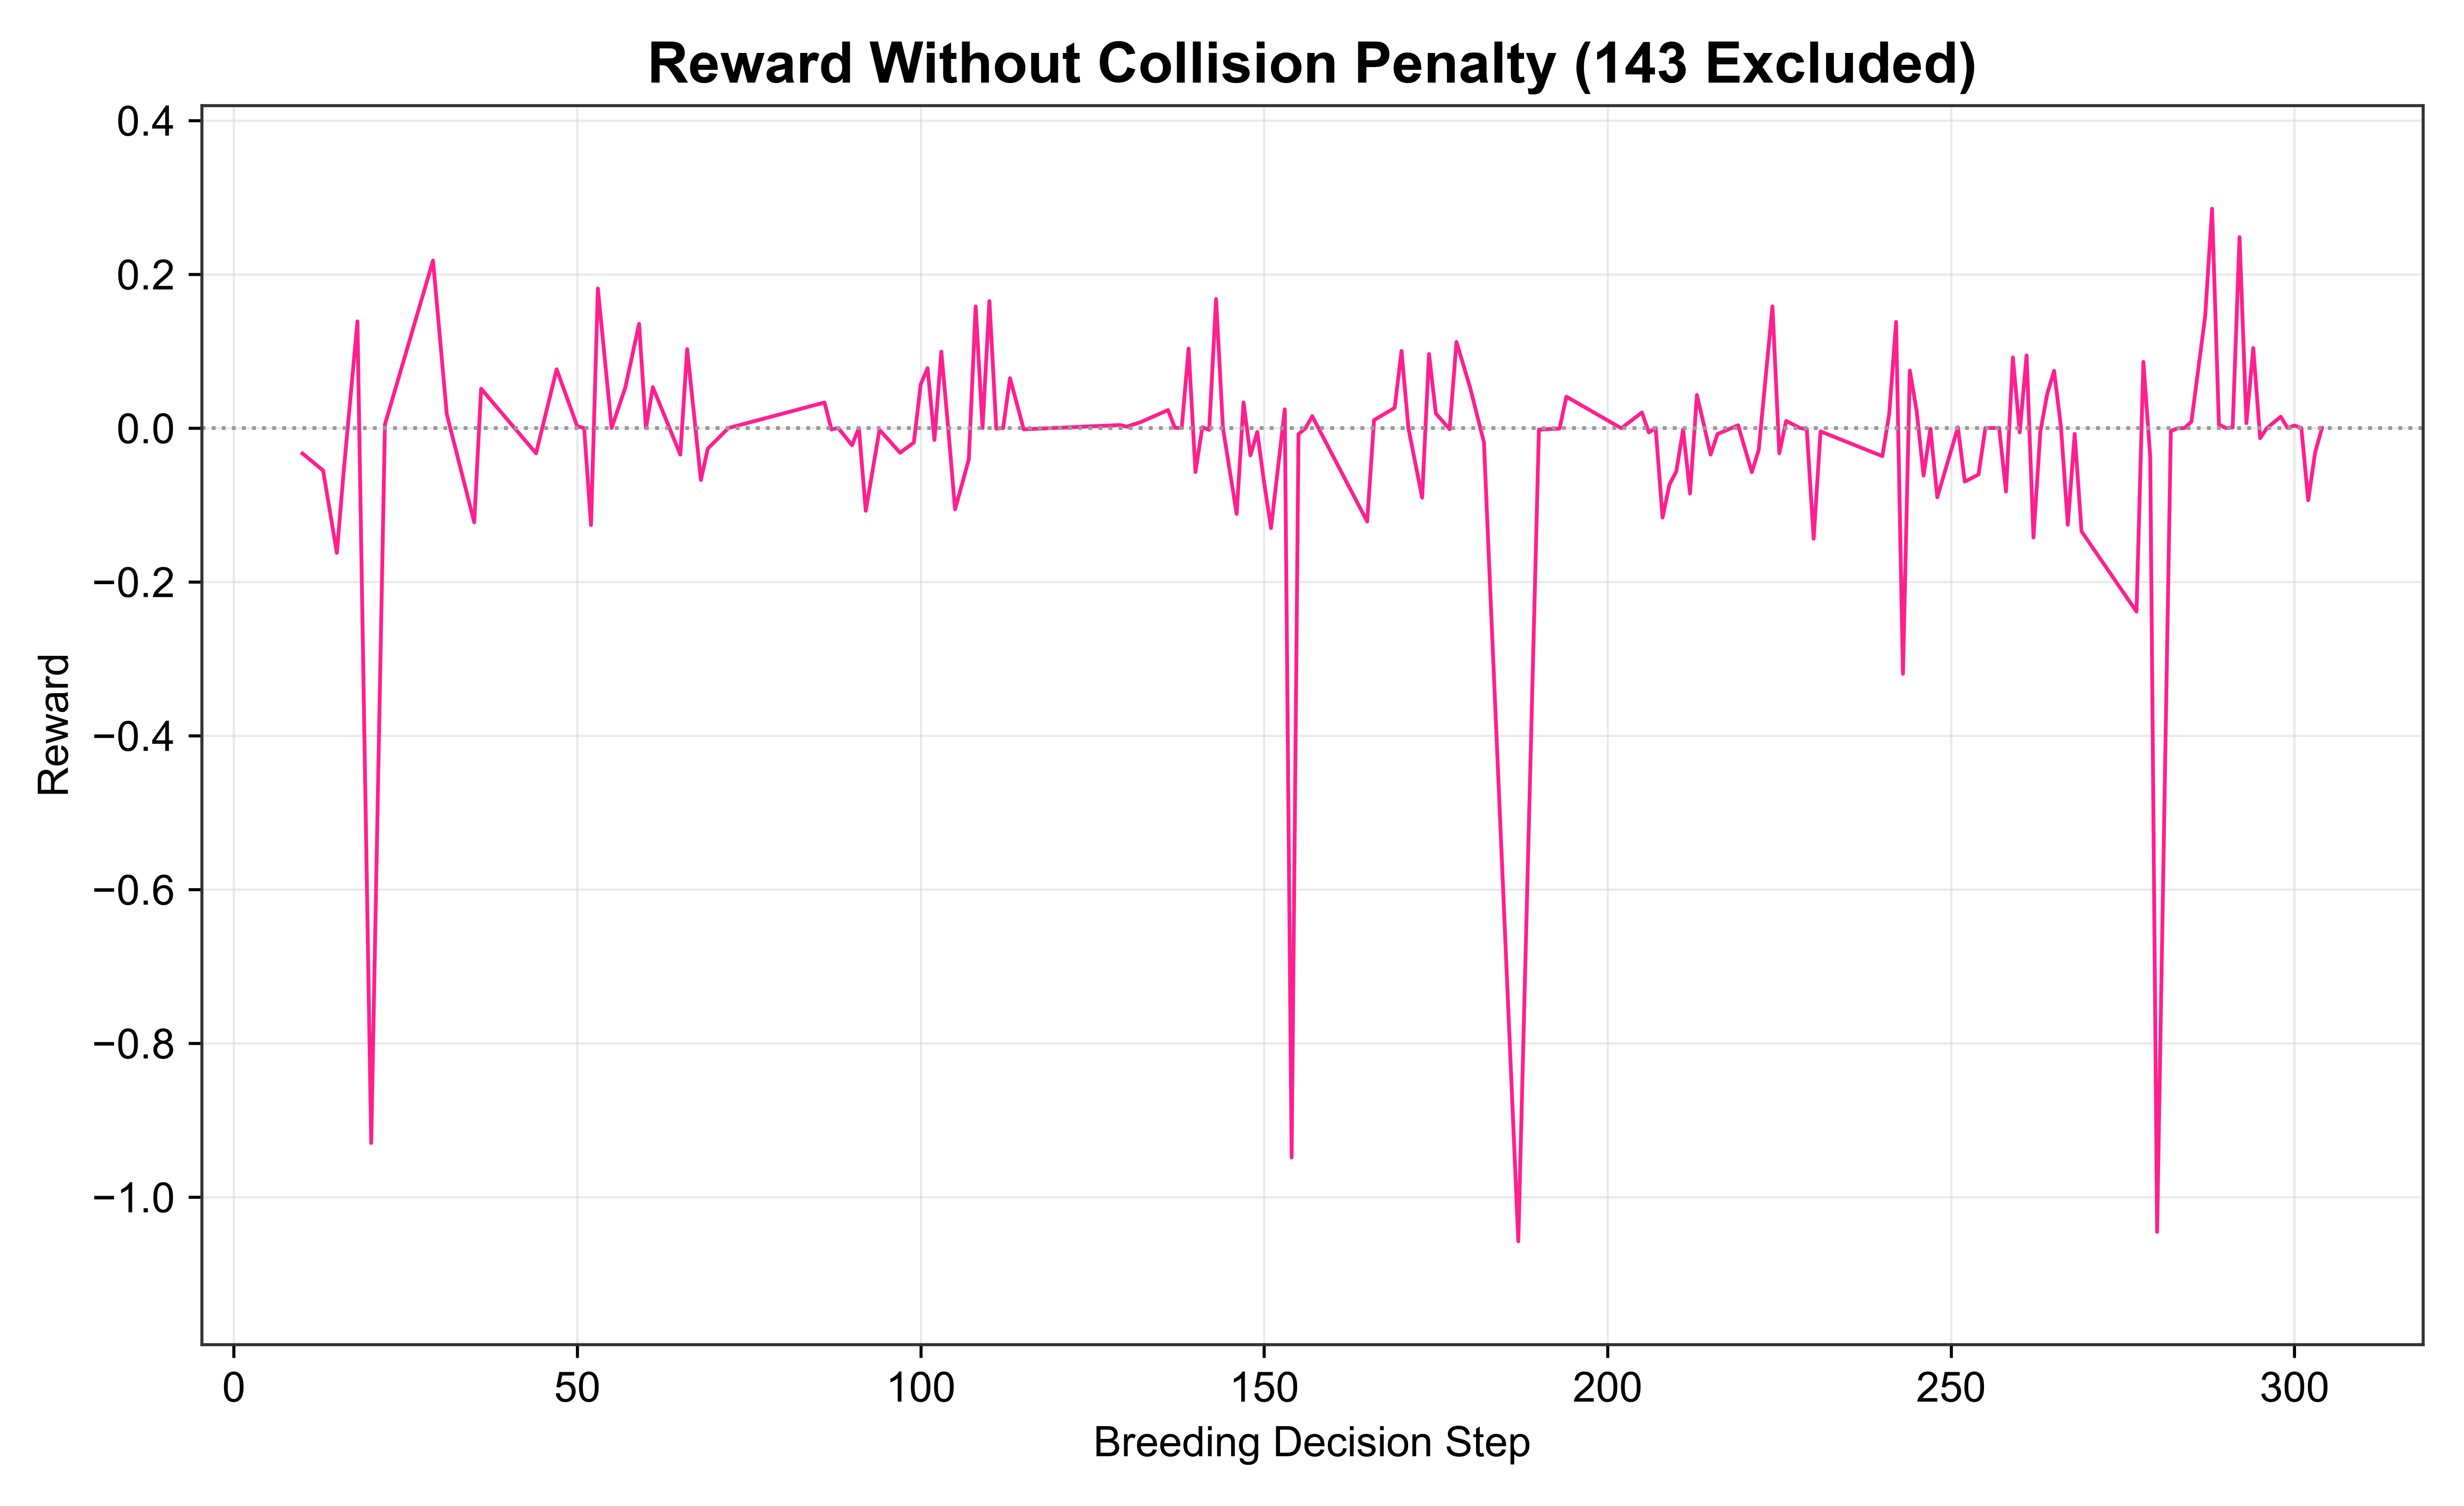
\includegraphics[width=\linewidth]{rl_diagnostics_reward_without_penalty.png}
        \caption{Reward per breeding decision}
    \end{subfigure}\hfill
    \begin{subfigure}[b]{0.48\linewidth}
        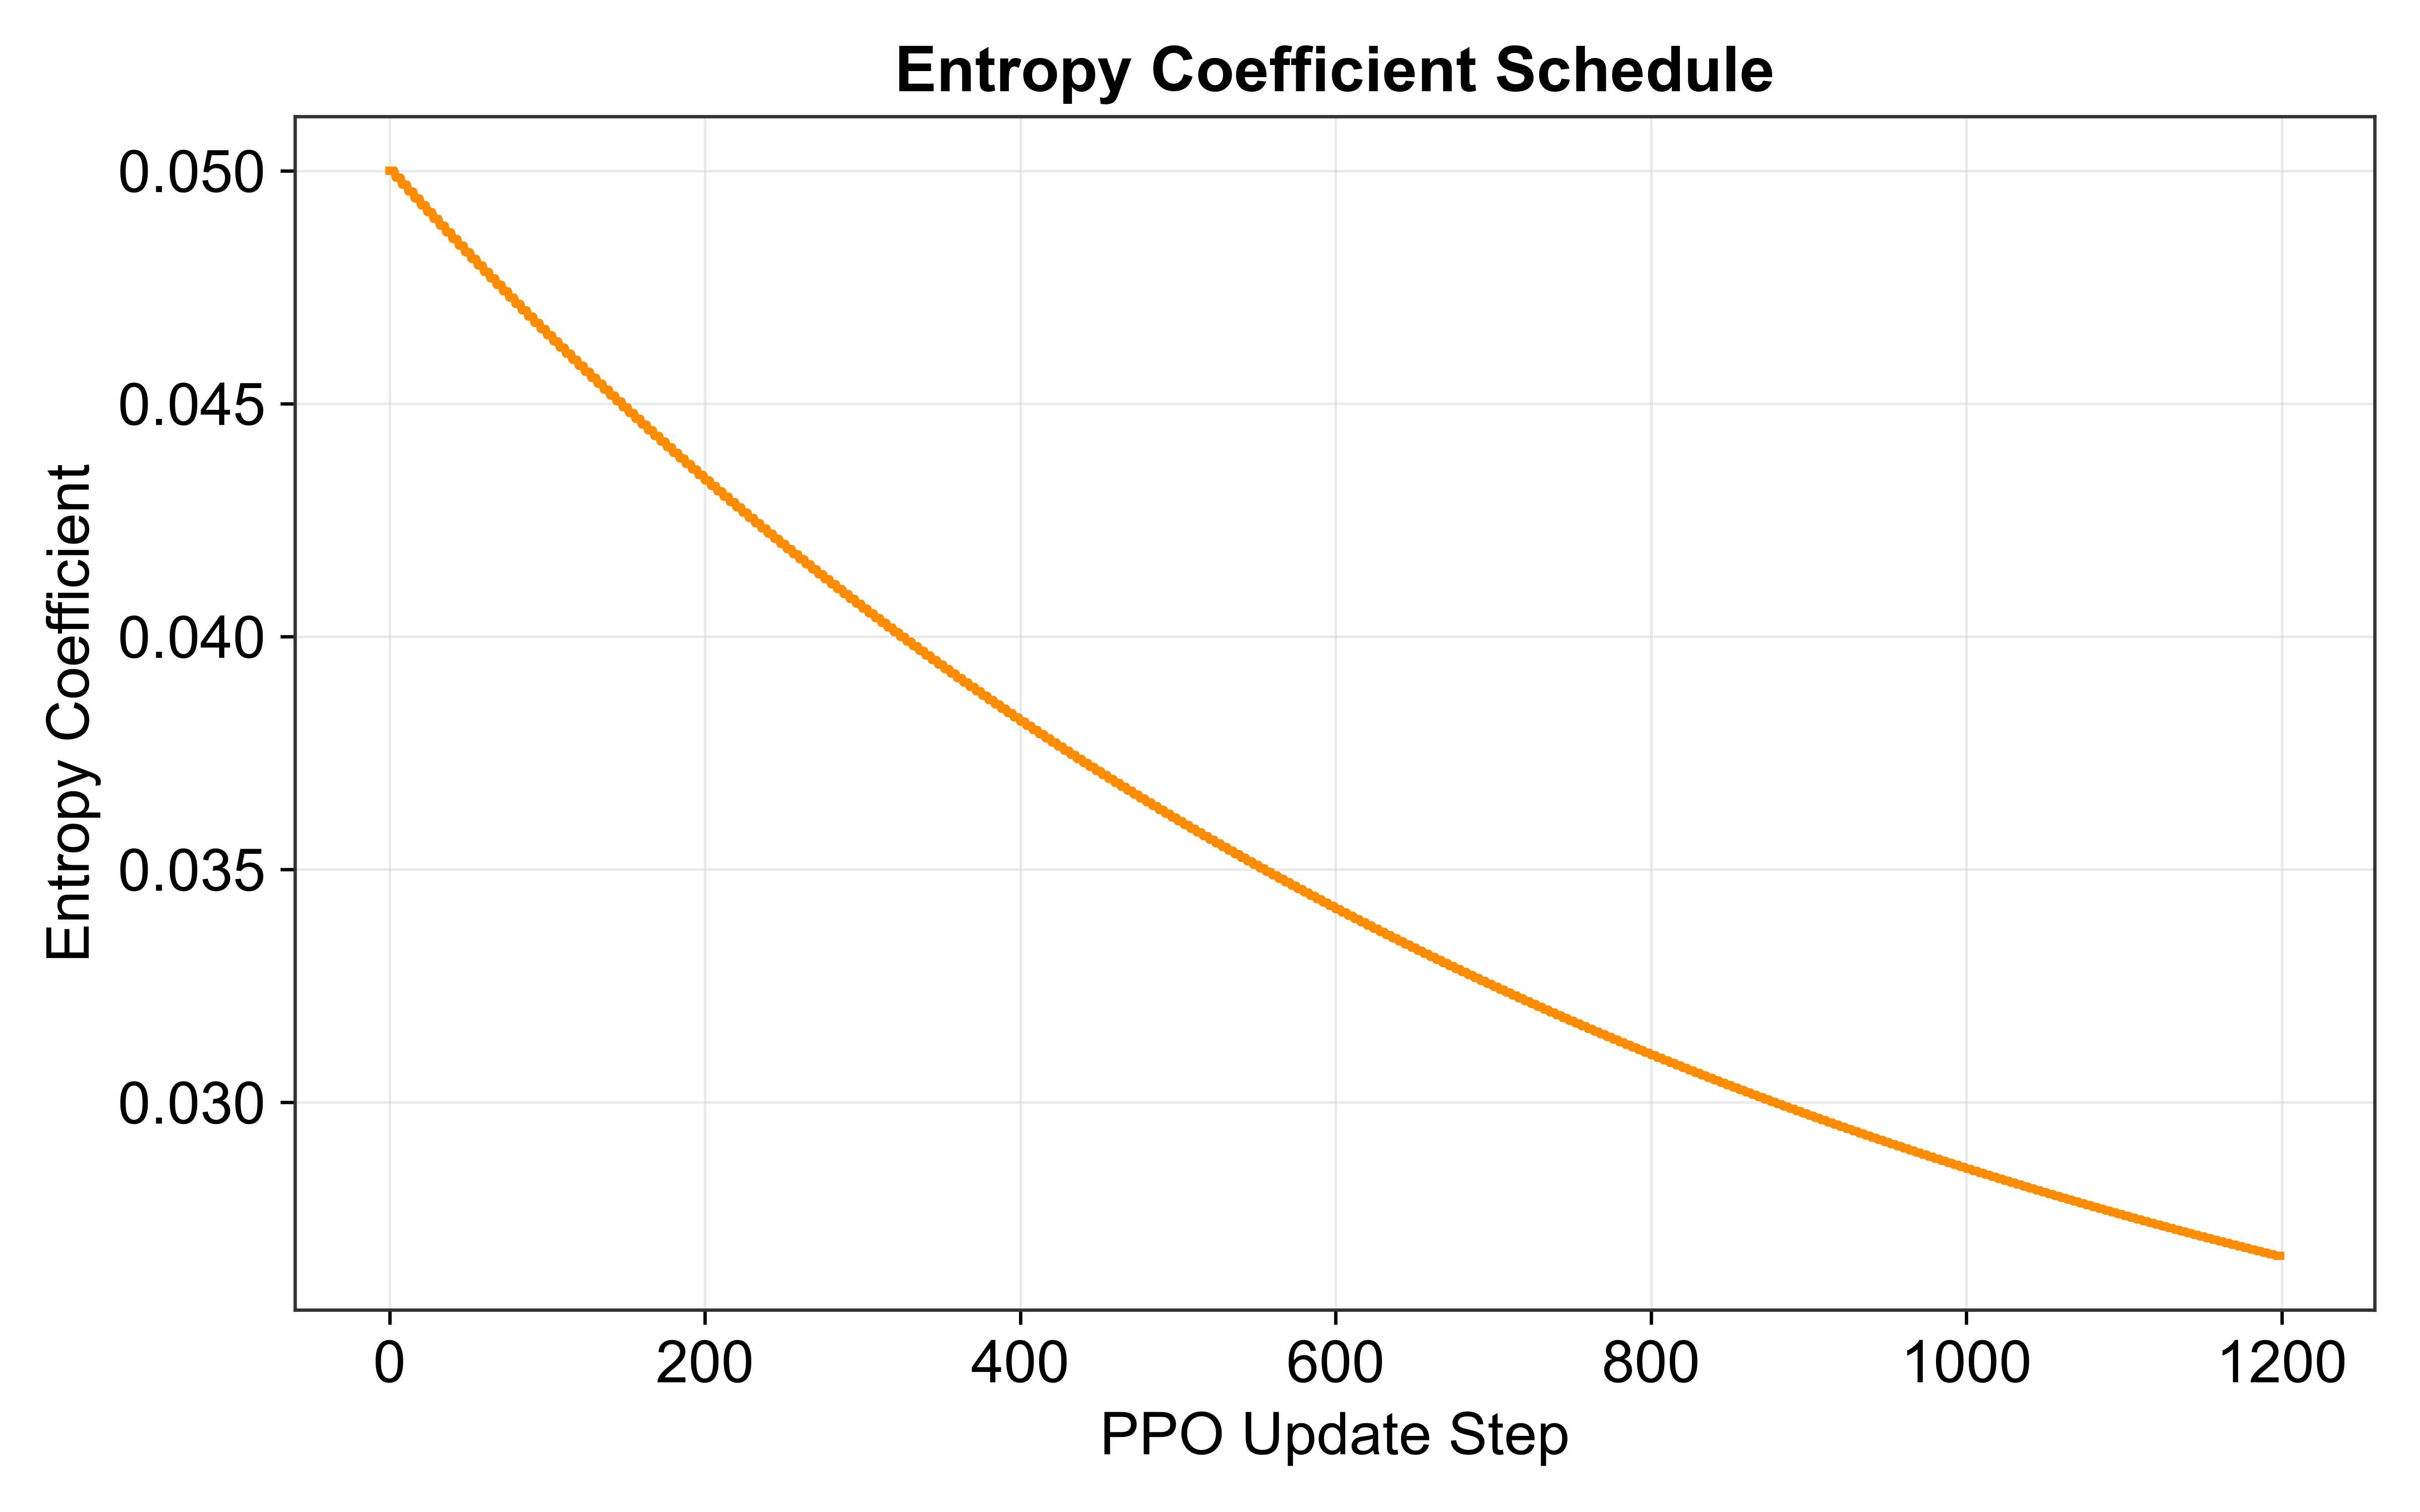
\includegraphics[width=\linewidth]{rl_diagnostics_entropy_coef.png}
        \caption{Entropy coefficient schedule}
    \end{subfigure}
    \par\vspace{0.6em}
    \begin{subfigure}[b]{0.48\linewidth}
        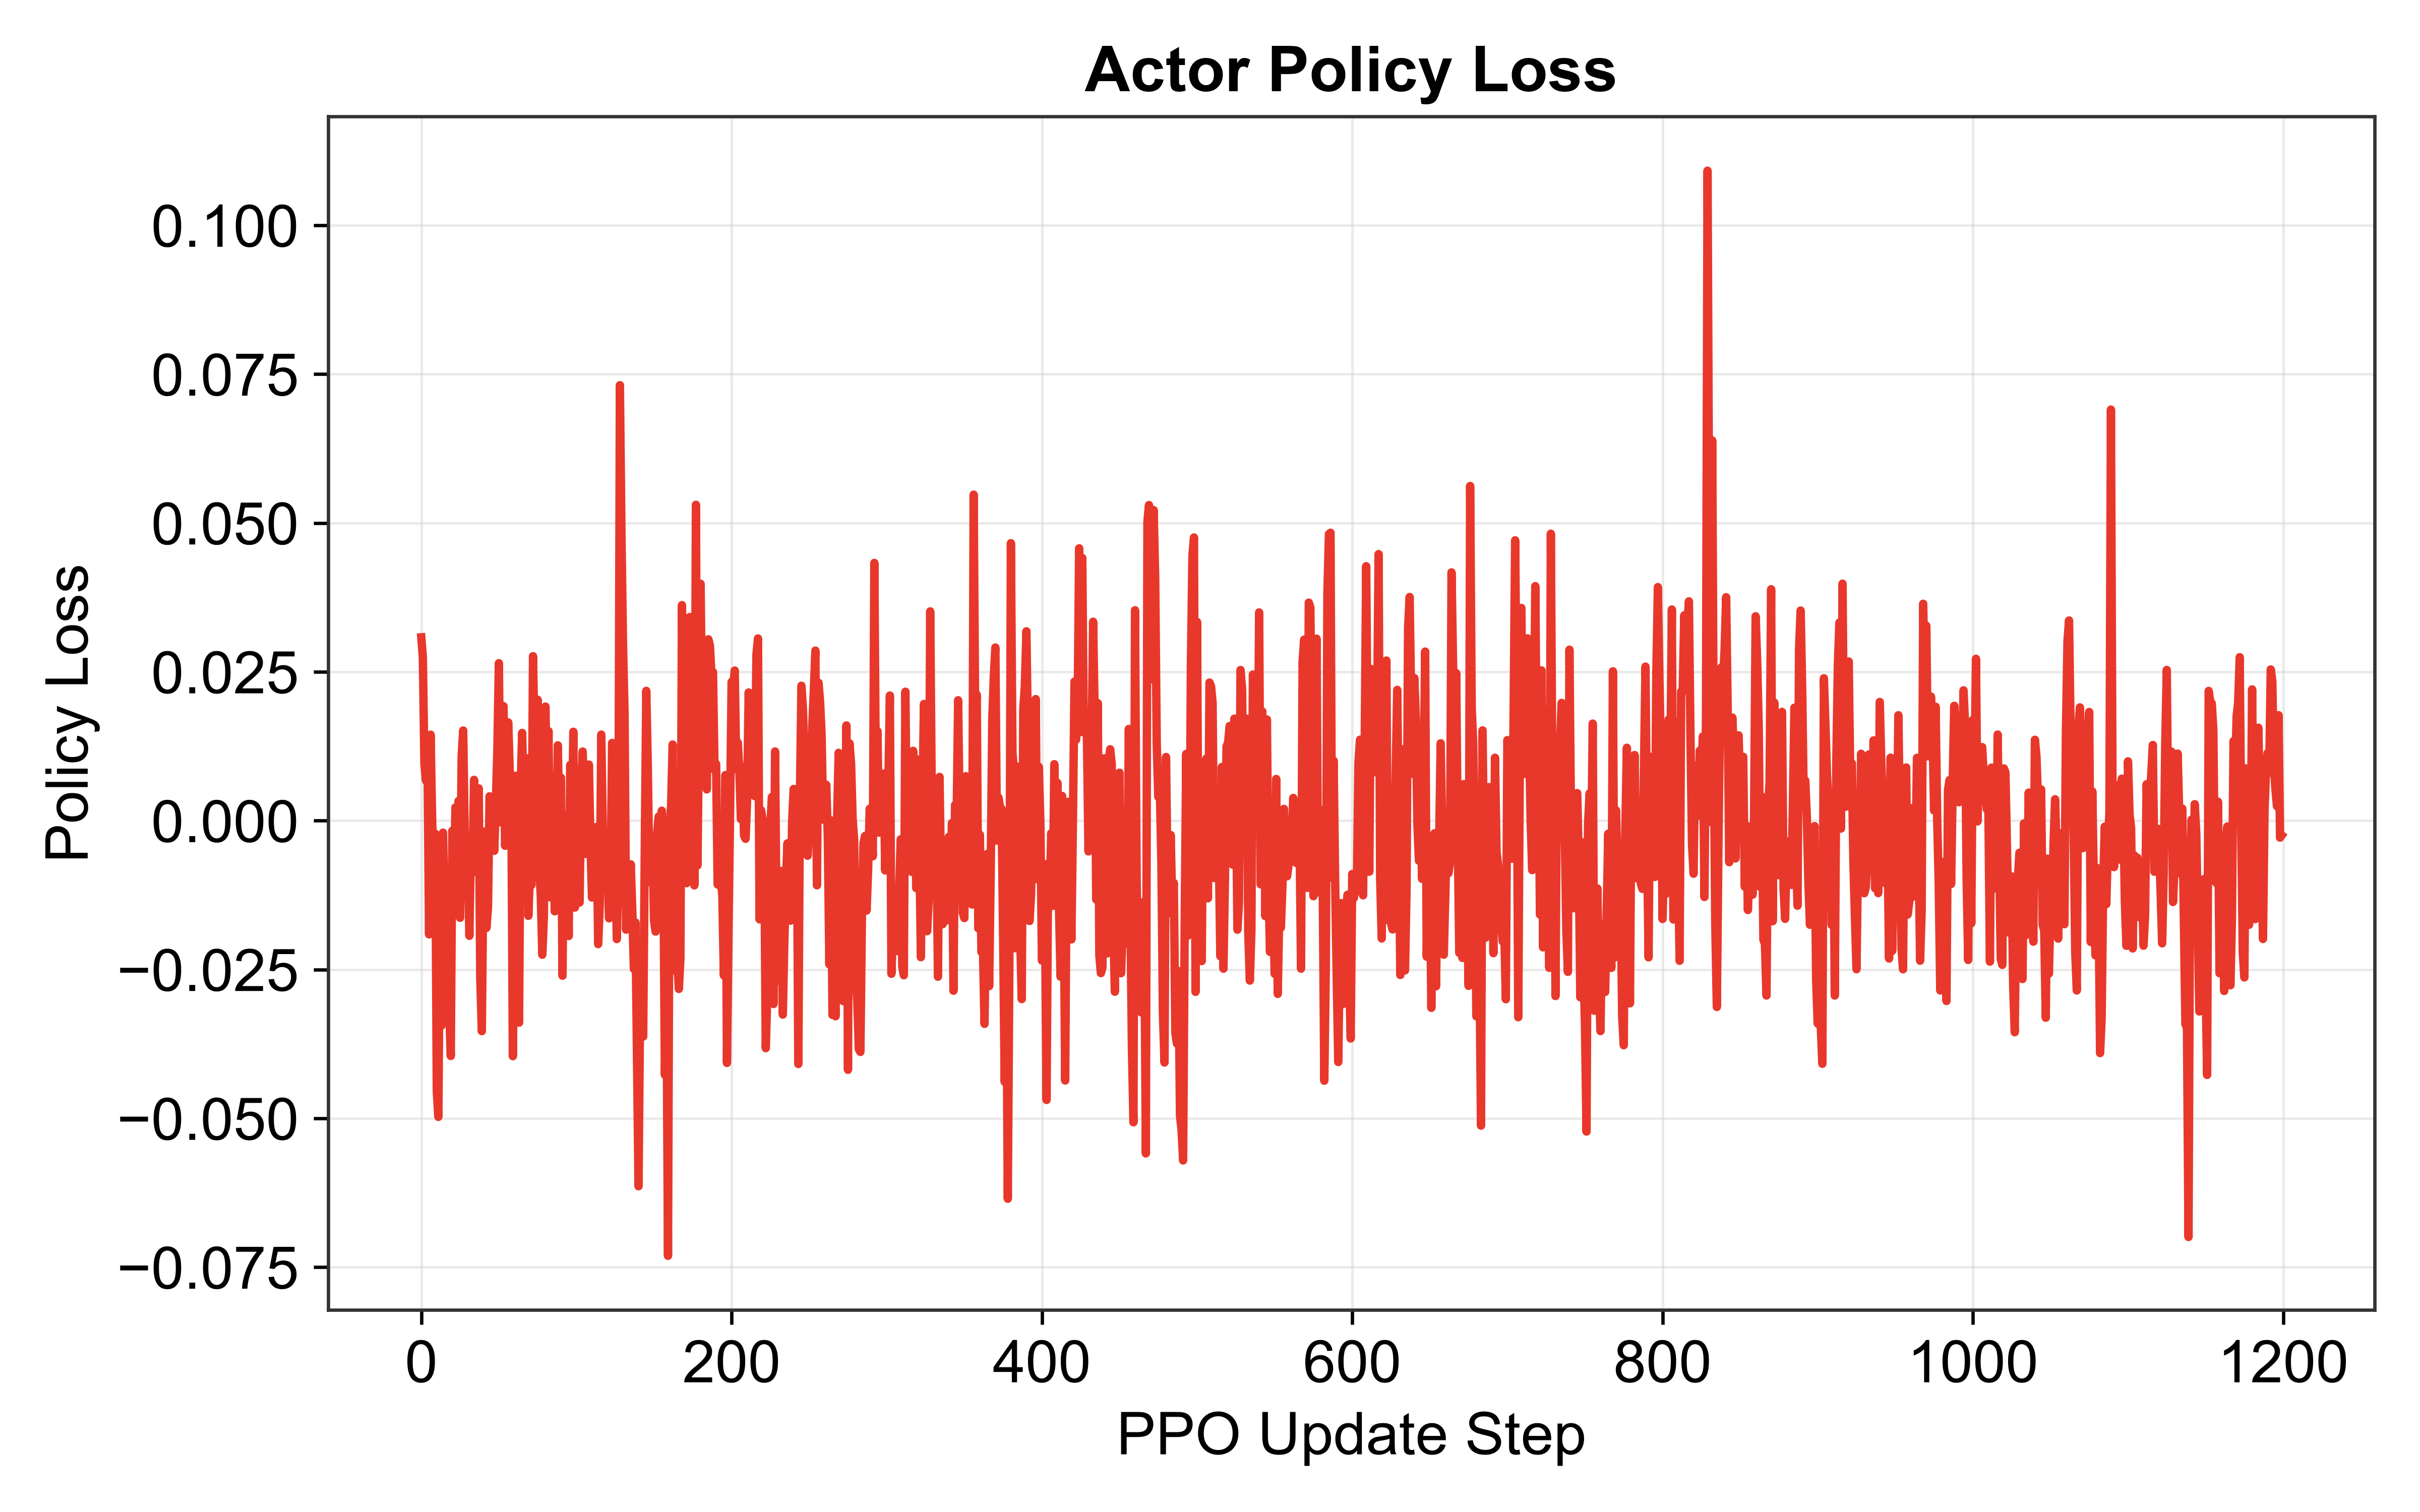
\includegraphics[width=\linewidth]{rl_diagnostics_policy_loss.png}
        \caption{Actor policy loss}
    \end{subfigure}\hfill
    \begin{subfigure}[b]{0.48\linewidth}
        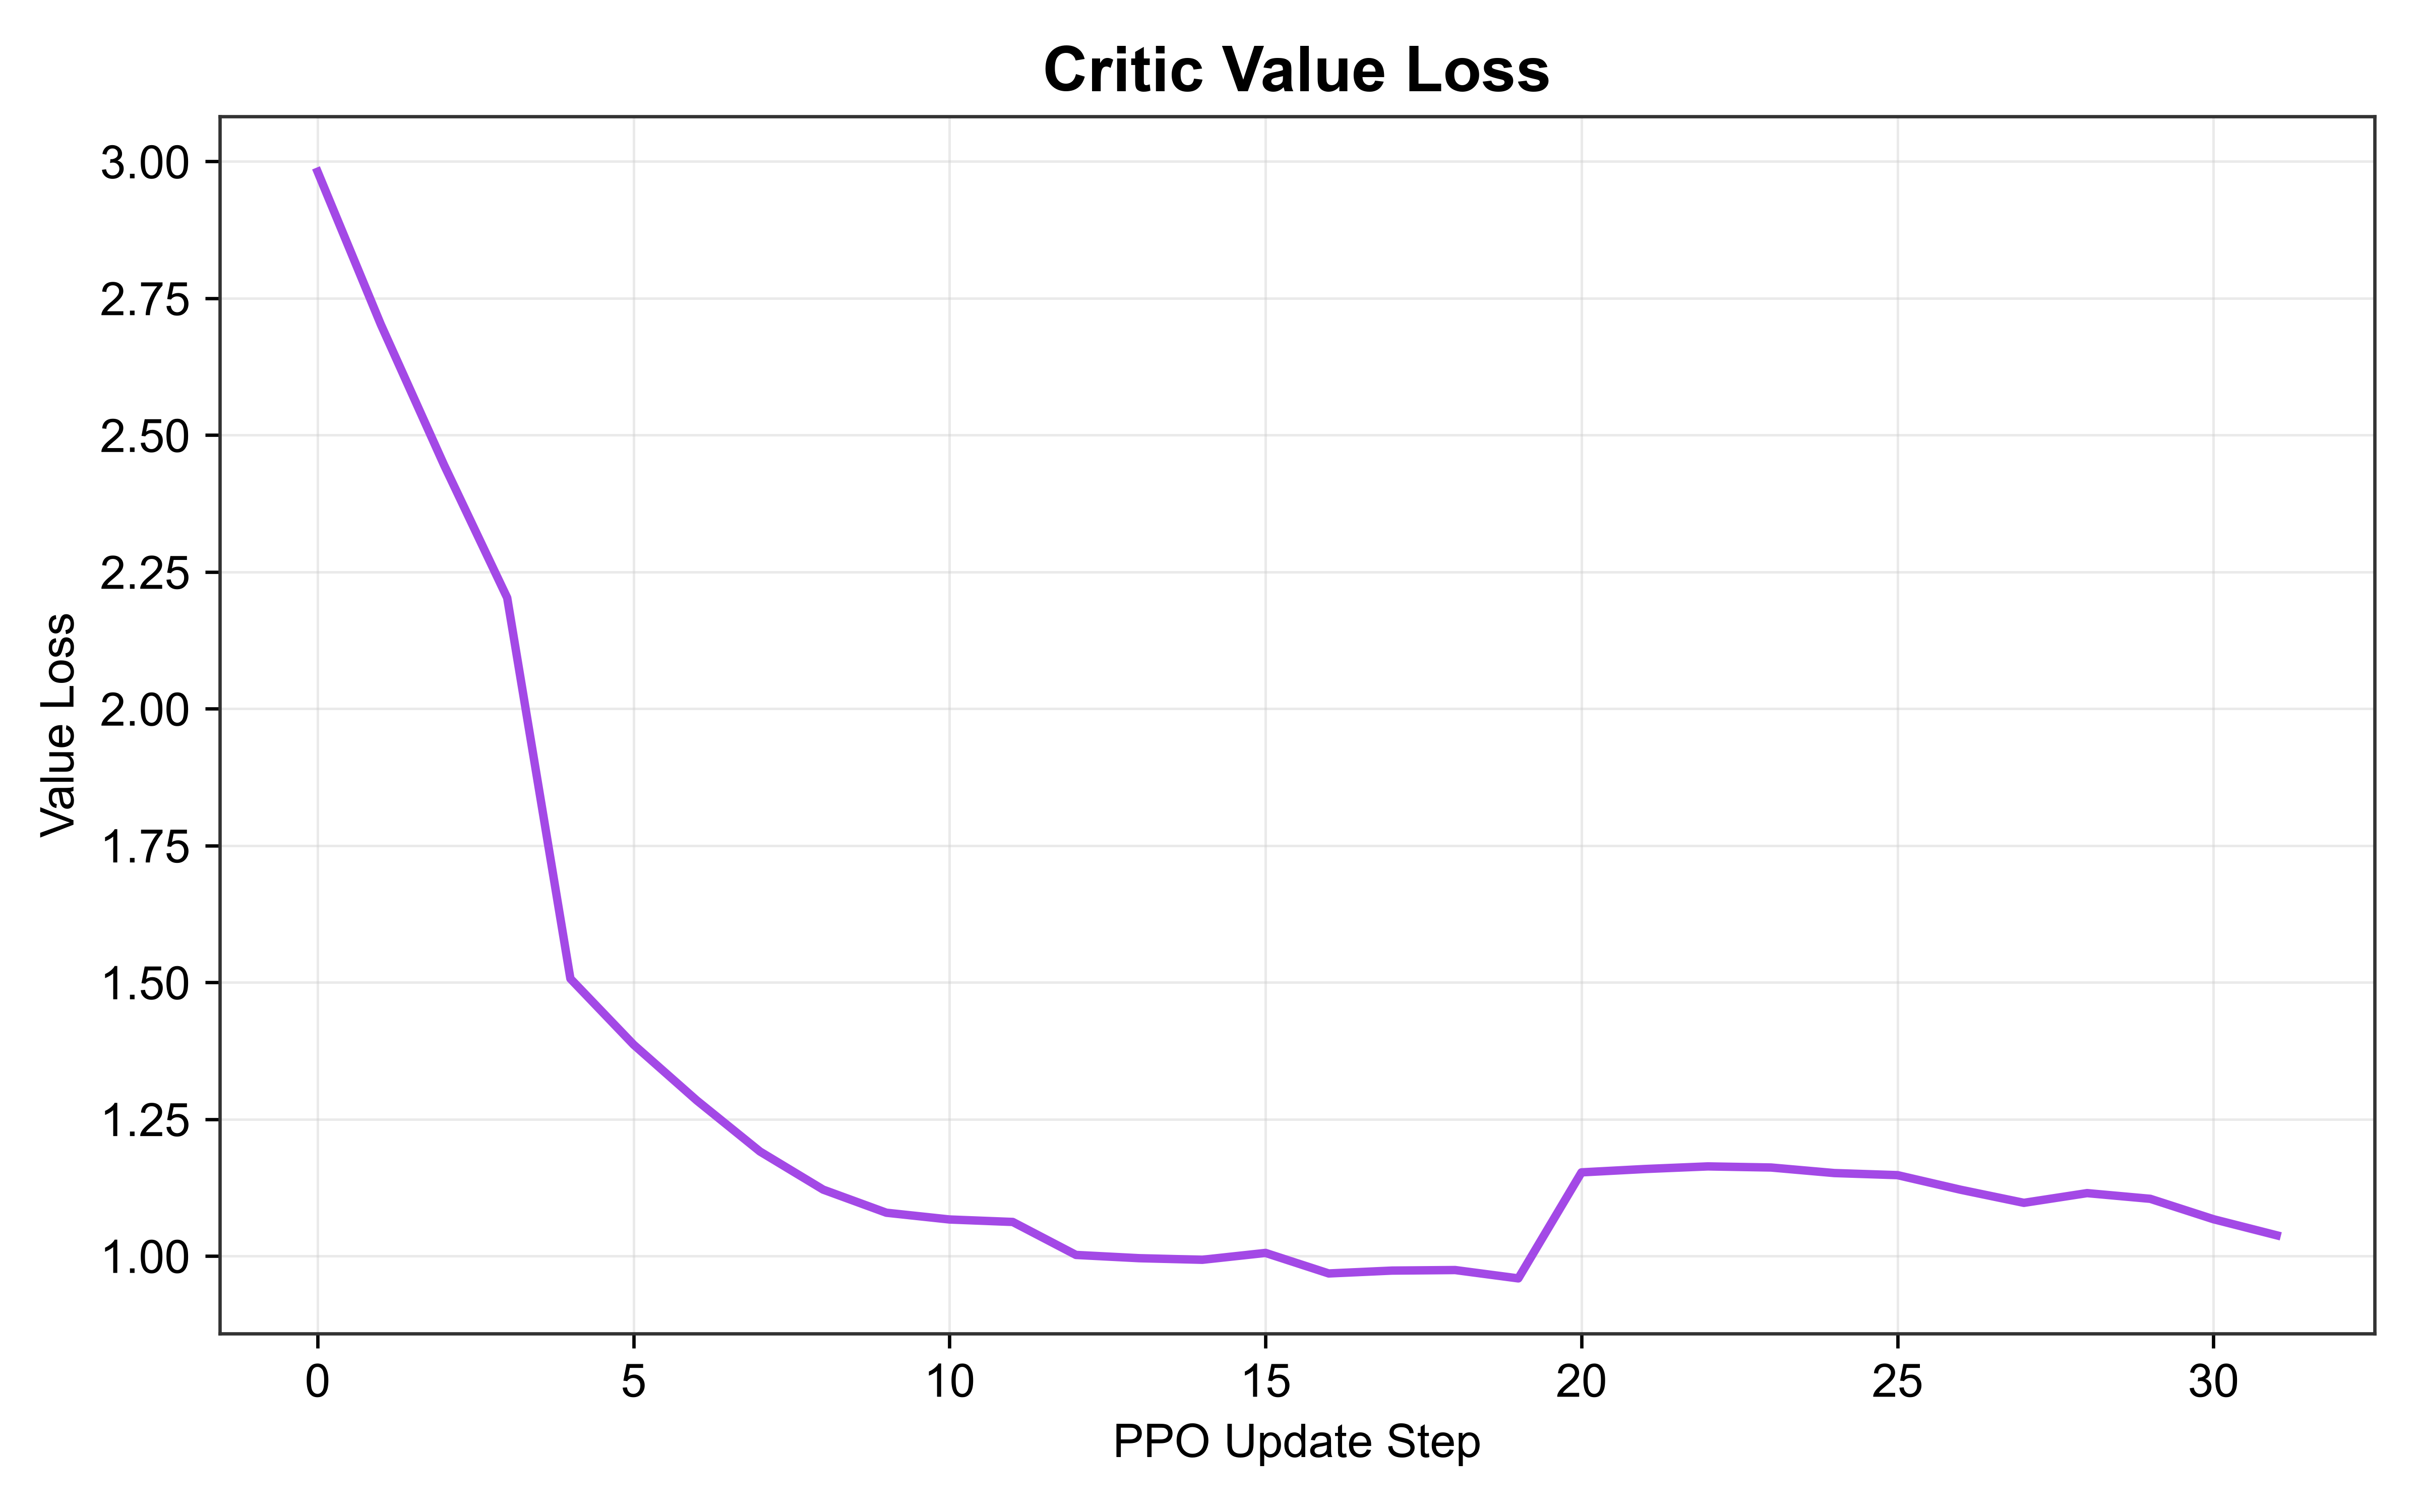
\includegraphics[width=\linewidth]{rl_diagnostics_value_loss.png}
        \caption{Critic value loss}
    \end{subfigure}
    \par\vspace{0.6em}
    \begin{subfigure}[b]{0.48\linewidth}
        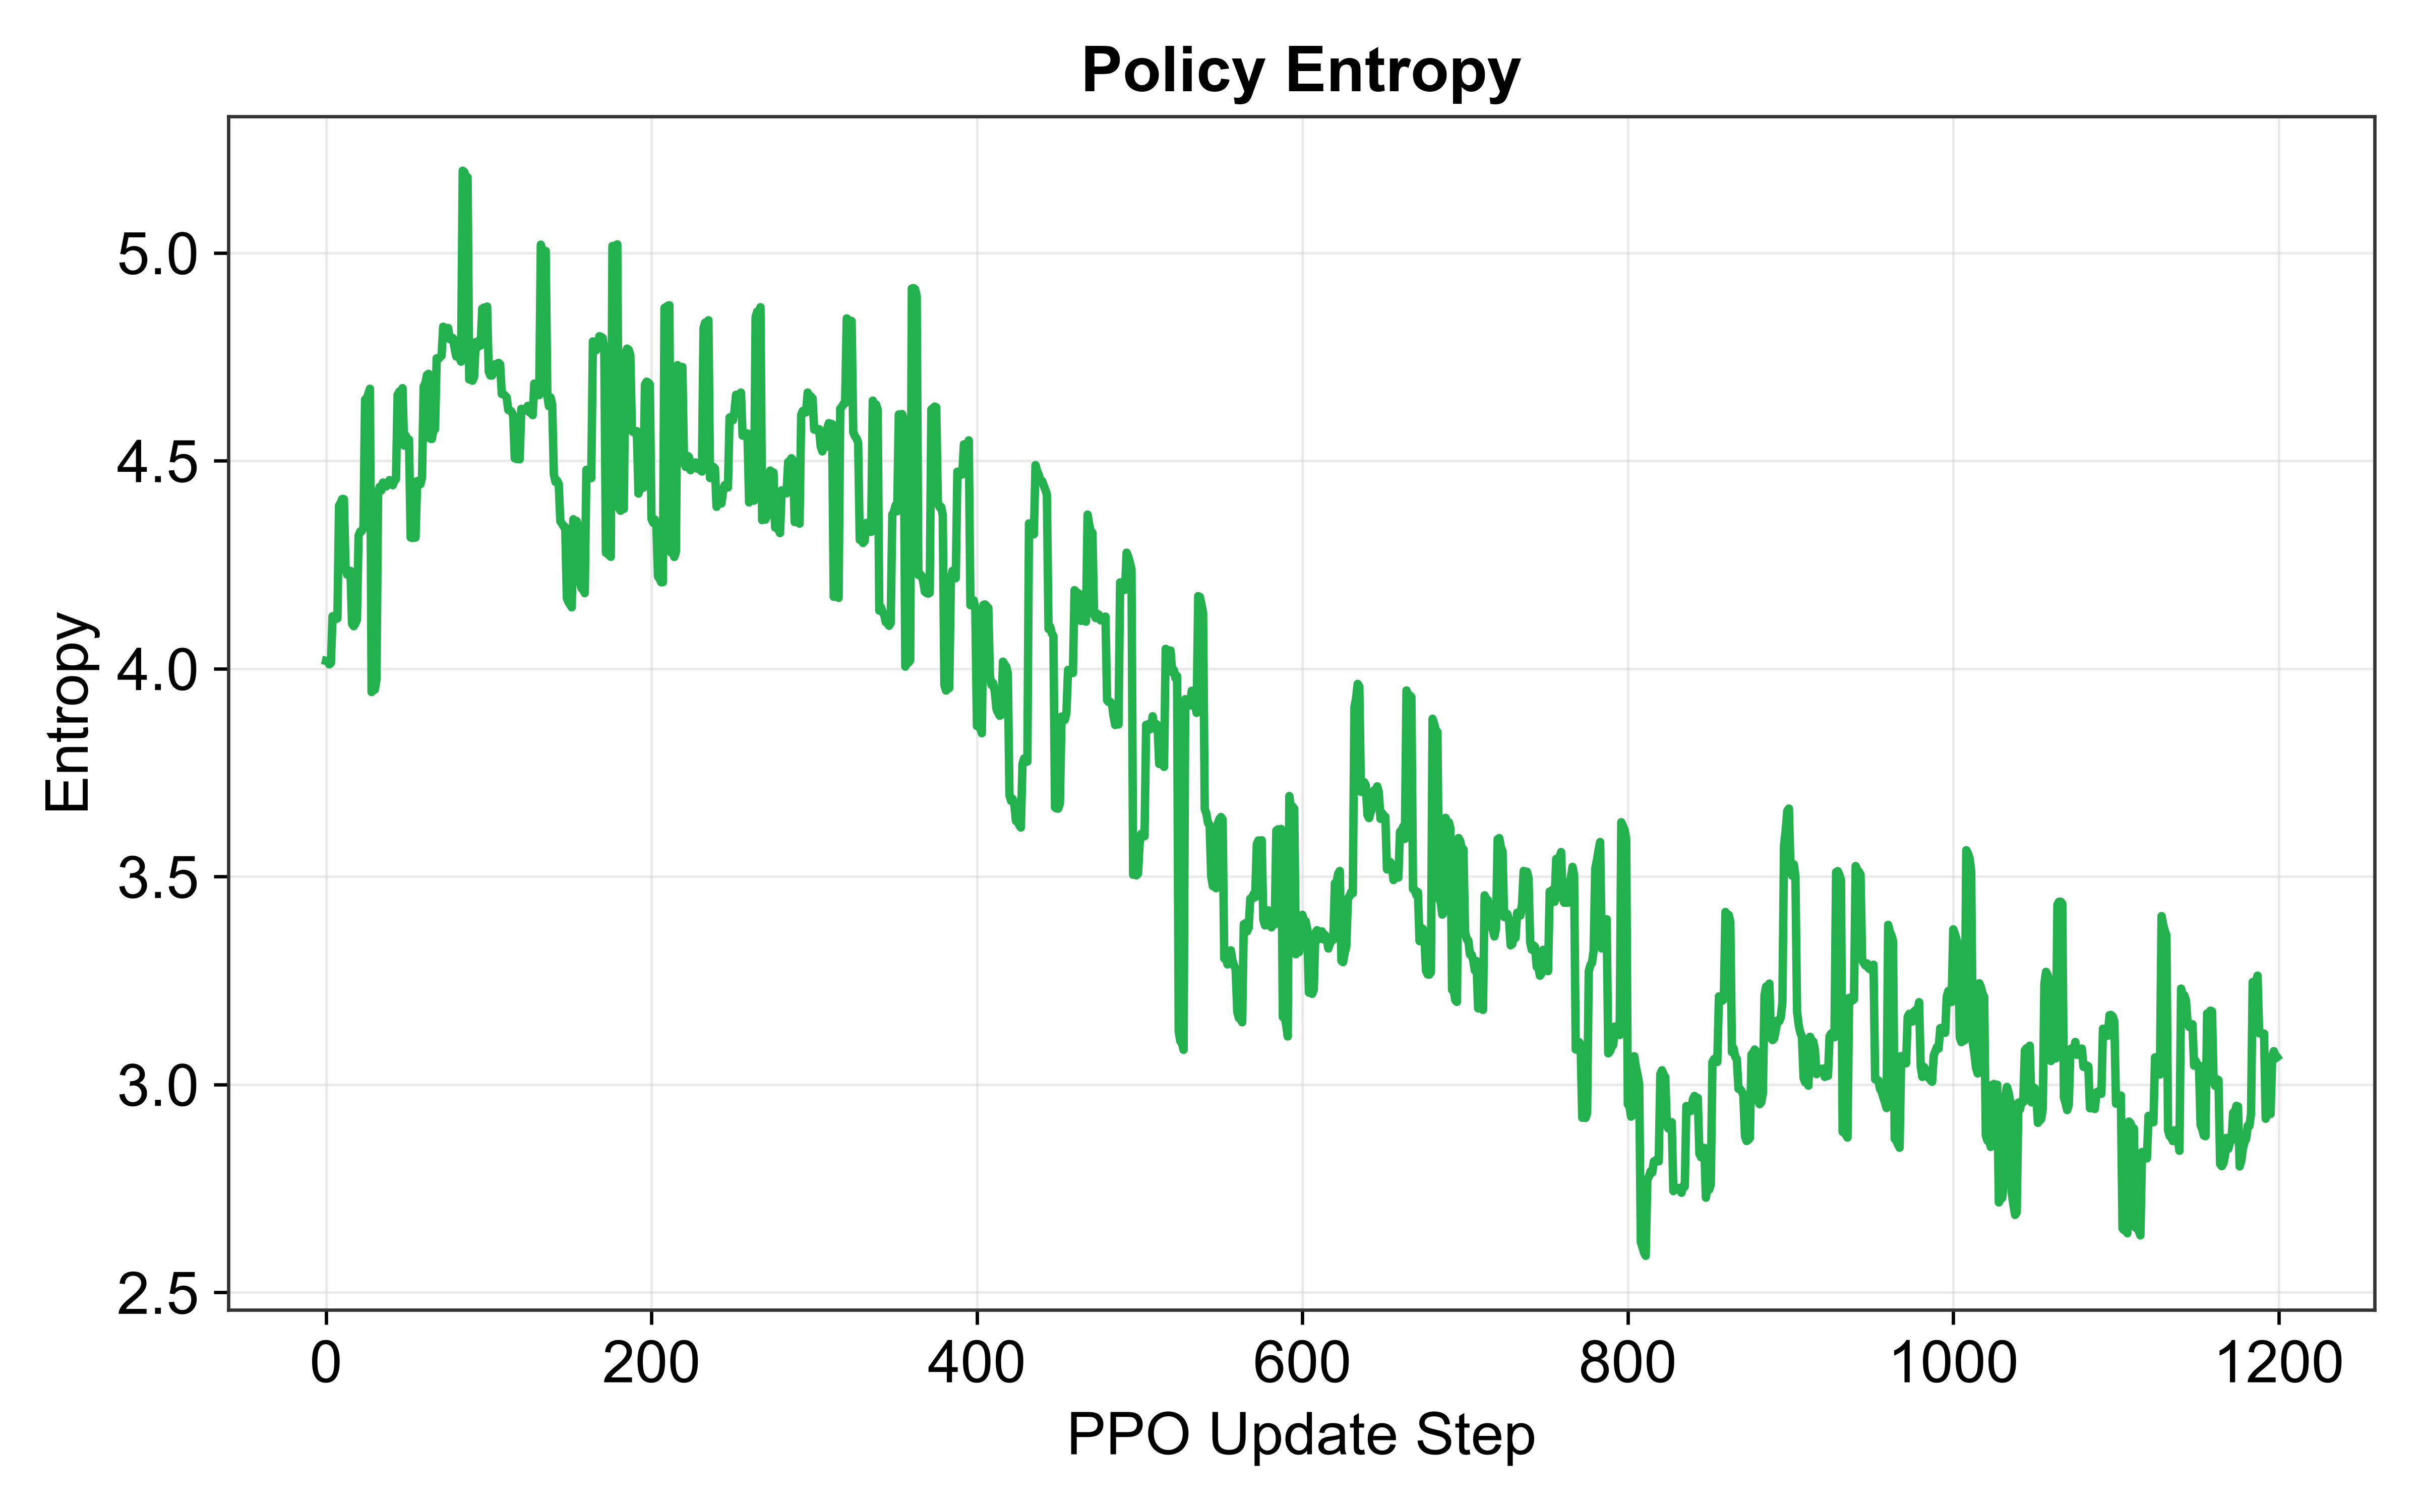
\includegraphics[width=\linewidth]{rl_diagnostics_entropy.png}
        \caption{Policy entropy}
    \end{subfigure}\hfill
    \caption{PPO training diagnostics across the 300-generation RL-assisted run.}
    \label{fig:rl-diagnostics}
\end{figure}
\begin{figure}[H]
    \centering
    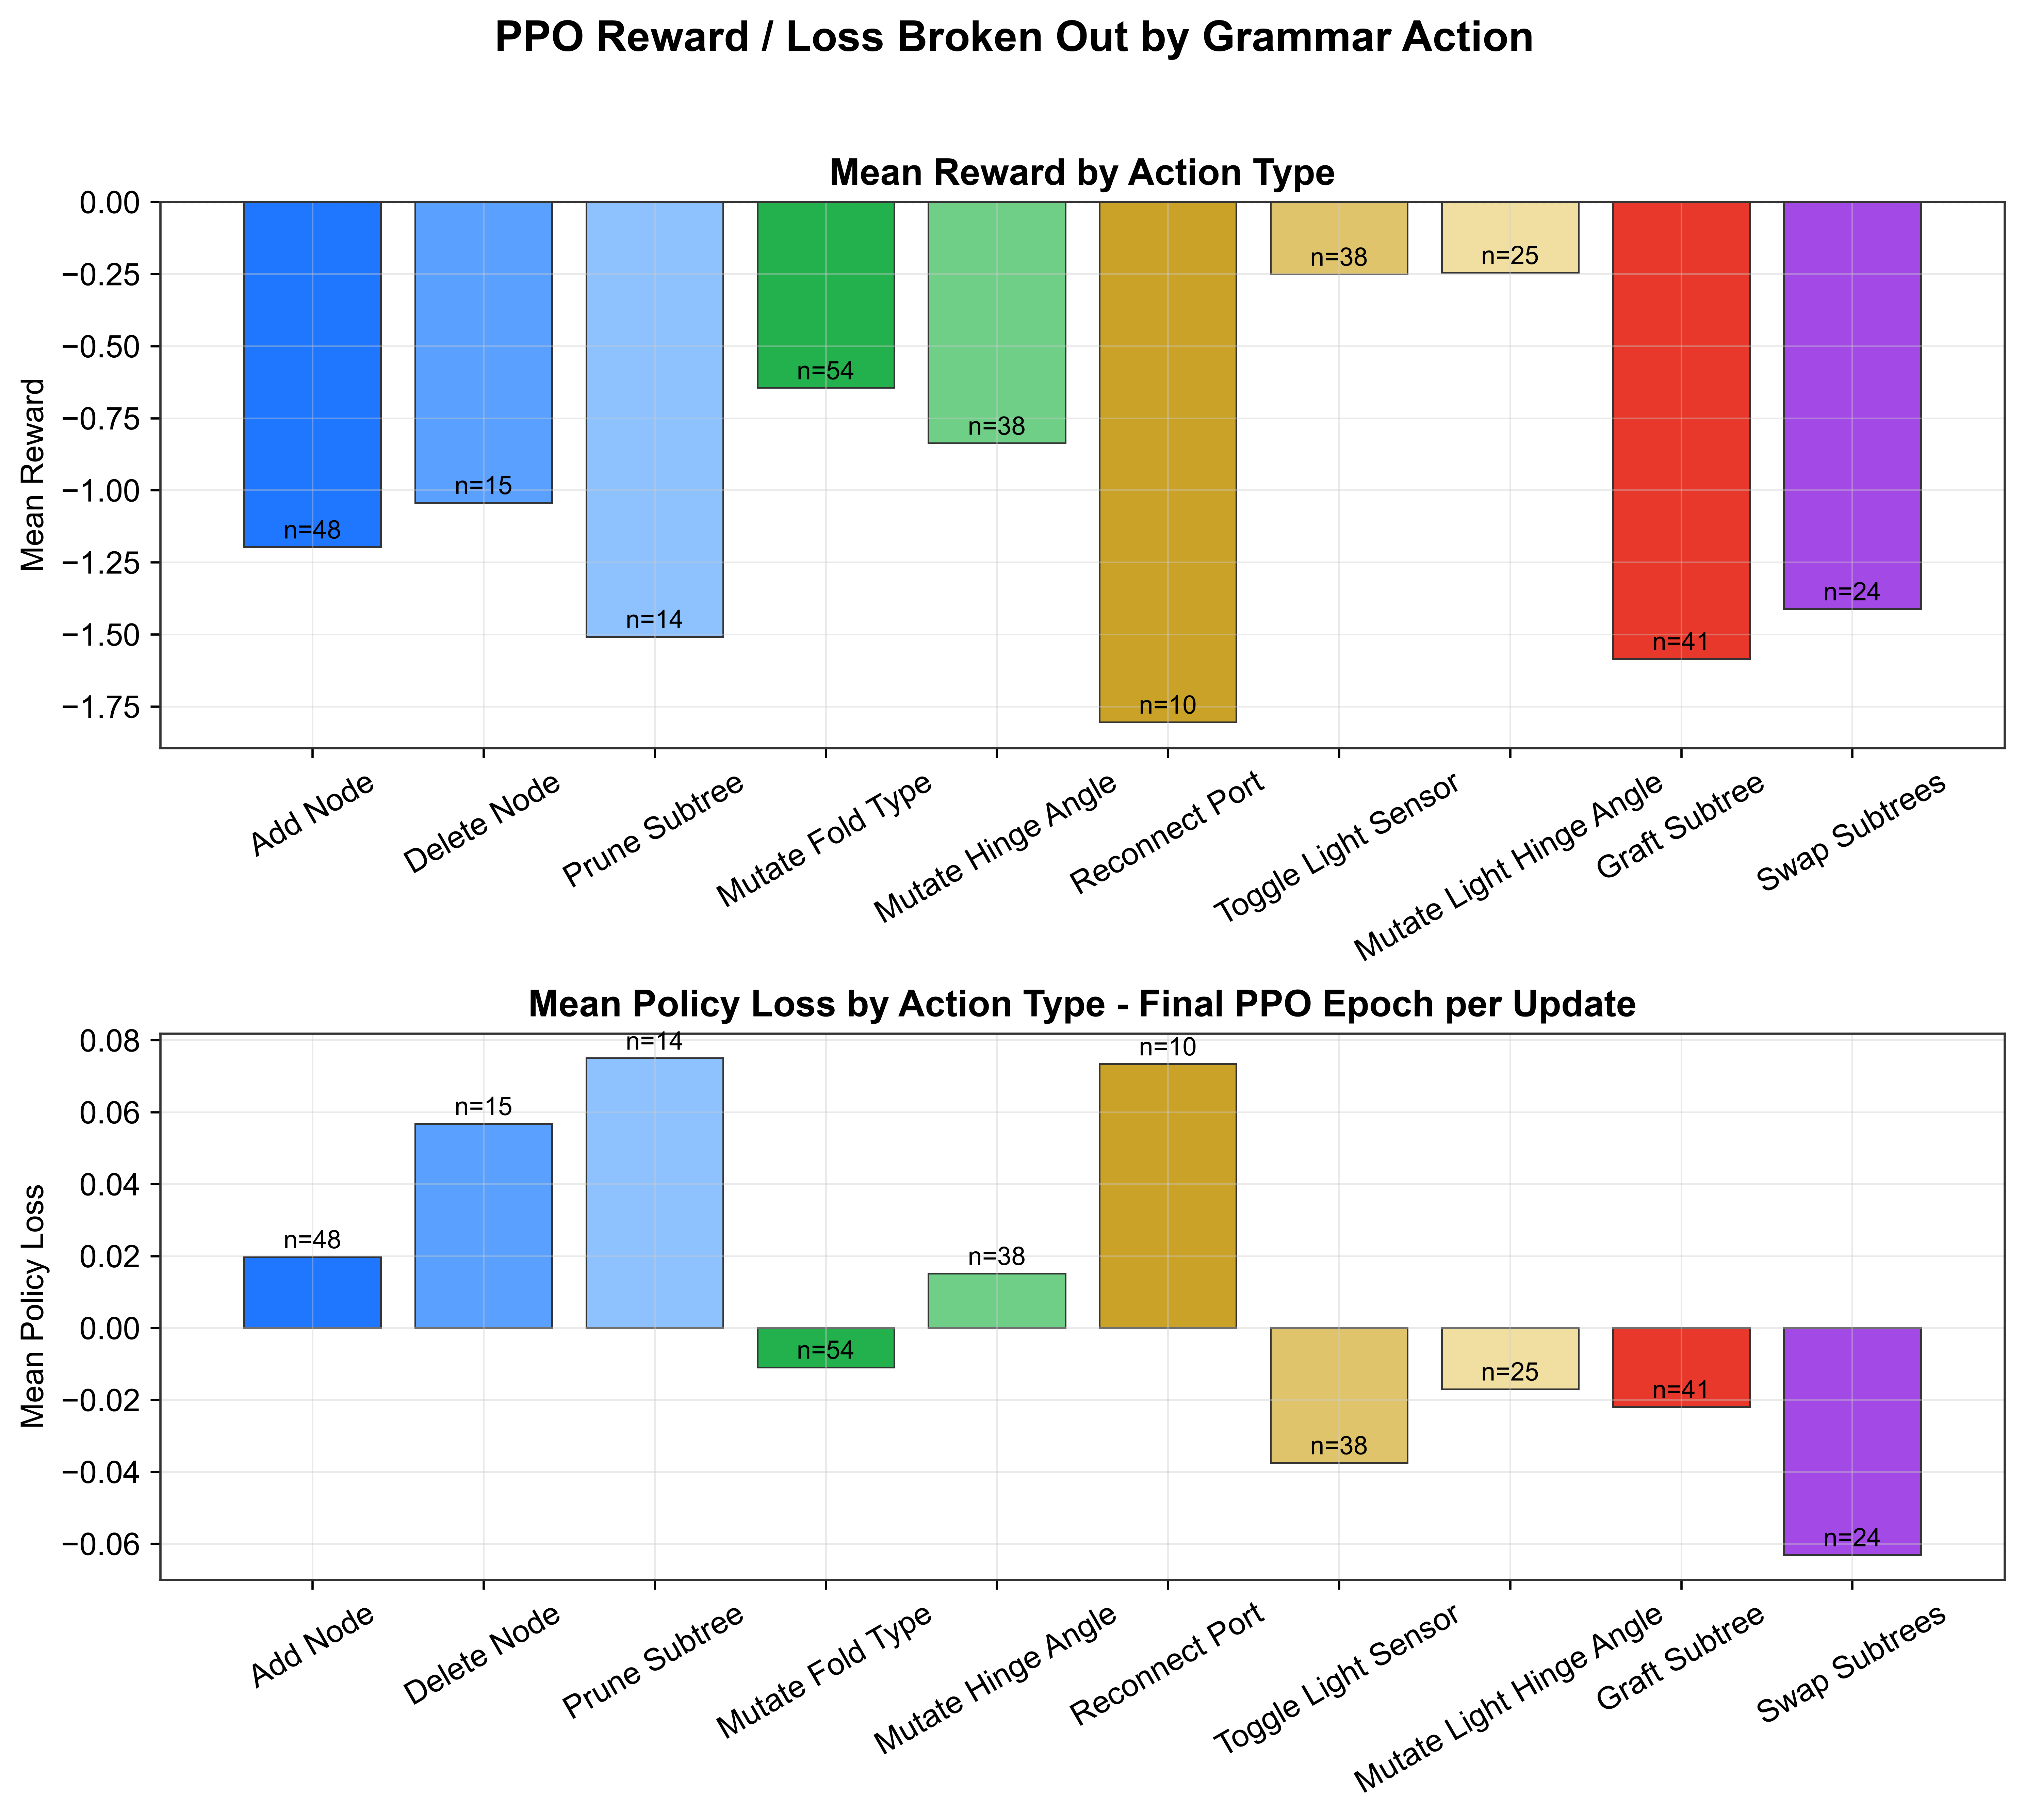
\includegraphics[width=0.85\linewidth]{rl_diagnostics_by_action.png}
    \caption{Mean reward and policy loss by grammar action type, aggregated over the run, with sample count $n$ per action.}
    \label{fig:rl-diagnostics-by-action}
\end{figure}

An earlier version of the actor-critic, at small scale, used a flat collision/instability penalty folded directly into the RL reward. This caused the crossover actions (Graft Subtree, Swap Subtrees) to collapse to near-zero selection probability within roughly the first ten generations, in both pheromone-response arms independently (Fig.~\ref{fig:rl-cp-action-distribution}): because every structural action carries some baseline collision risk while several non-structural actions (e.g.\ Toggle Light Sensor) structurally cannot ever trigger the collision gate, any reward mechanism that lets the policy compare outcomes across action types will discover and exploit that asymmetry, regardless of how the penalty itself is scaled. This is why collision and instability outcomes were removed from the reward stream entirely for the architecture used to produce the results in this thesis (Section~\ref{sec:rl-actor-critic}), rather than reduced, reshaped or bounded per action type.

Consistent with that redesign, Fig.~\ref{fig:action-distribution-both} shows no equivalent collapse in the 300-generation run: all ten actions remain in use throughout. The per-action breakdown (Fig.~\ref{fig:rl-diagnostics-by-action}) shows every action type has a negative mean reward over the run (roughly $-0.03$ to $-0.19$), which is expected because most individual breeding decisions do not improve on their own parent; Mutate Hinge Angle and Prune Subtree have the most negative mean reward (both around $-0.18$ to $-0.19$), while Toggle Light Sensor and Reconnect Port are closest to zero (around $-0.03$ to $-0.05$). Sample counts range from $n=318$ (Graft Subtree) to $n=1853$ (Reconnect Port) across the whole run, confirming that crossover actions are used consistently but remain a minority of decisions relative to the mutation actions. The reward trace (Fig.~\ref{fig:rl-diagnostics}a) is highly variable step-to-step and, read by eye across the full run, does not show a clear rising trend; policy entropy (Fig.~\ref{fig:rl-diagnostics}e) declines gradually from an initial range of about 4.0--5.2 to about 2.7--3.5 by the run's end, indicating the policy becomes more peaked over training without collapsing toward a single action, consistent with the sustained ten-action usage in Fig.~\ref{fig:action-distribution}. Critic value loss (Fig.~\ref{fig:rl-diagnostics}d) falls sharply within the first approximately 50 PPO updates and then continues a slow, noisy decline; actor policy loss (Fig.~\ref{fig:rl-diagnostics}c) stays noisy around zero throughout with a small number of larger spikes, without a clear systematic trend, which is not unusual for PPO's clipped-surrogate objective.

Because the collision penalty has been removed from the reward stream, the per-action-type reward-normalisation idea previously proposed as a fix specifically for the old collision-driven collapse is no longer directly applicable in that form. The residual action-type imbalance visible above -- crossover actions receiving roughly a fifth to a sixth of the samples of the most common mutations (Fig.~\ref{fig:rl-diagnostics-by-action}) -- means their reward and advantage estimates are still based on substantially less evidence than the common mutation actions', which is proposed in Section~\ref{ch:conclusion} as a more general direction: not fixing a collision-specific asymmetry, but giving the policy a comparably reliable reward signal for the actions it samples least often.


\chapter{Discussion}
\label{ch:discussion}
This chapter draws the results of Chapter~\ref{ch:results} together against the aims and objectives set out in Chapter~\ref{ch:introduction}, considering each in turn rather than presenting new evidence. Section~\ref{sec:disc-basic} addresses the basic objectives O-1 to O-4, and Section~\ref{sec:disc-advanced} addresses the advanced objectives AO-1 and AO-2.

\section{Basic Objectives (O-1 to O-4)}
\label{sec:disc-basic}
O-1 was achieved with a qualified result. The graph policy and its integration were implemented, and the 300-generation comparison in Section~\ref{sec:rl-vs-random} shows a mixed outcome rather than a clean win or loss for the RL-assisted arm: it reaches a higher best individual velocity and speed response than standard breeding, and a substantially lower collision rate from around generation 140 onward, but standard breeding maintains a consistently higher hypervolume throughout the run and a modestly higher scalarised best fitness in the run's final third (Figs.~\ref{fig:fitness-trends-comparison}--\ref{fig:collision-rate-comparison}). The diagnostic analysis in Section~\ref{sec:rl-diagnostics} adds that, once collision outcomes were excluded from the reward stream, the earlier action-collapse failure mode did not recur over the full 300 generations, though crossover actions remain a persistent minority of decisions with correspondingly less reward evidence behind them. O-1's specific ML approach has therefore been implemented and evaluated in detail at full scale, but it has not been shown to uniformly outperform the random baseline it was intended to improve on -- it outperforms on some measures and underperforms on others, most notably the primary many-objective convergence measure. A same-generation-budget, multi-seed comparison remains the clearest way to resolve this, and is proposed as future work (Section~\ref{ch:conclusion}). O-2 and O-3 were achieved at simulation level: legal graphs were folded, actuated and scored in MuJoCo, as illustrated by the evolved assemblies in Fig.~\ref{fig:evolved-morphologies-both}. O-4 was addressed through the convergence, hypervolume and Pareto analyses (Figs.~\ref{fig:convergence}, \ref{fig:hypervolume} and \ref{fig:pareto-front}); hypervolume was still rising at the end of the 300-generation run, so this evidence supports the framework's operation without establishing long-term convergence.

\section{Advanced Objectives (AO-1 and AO-2)}
\label{sec:disc-advanced}
AO-1 was changed and achieved through the attractive and repulsive pheromone-response objectives and their morphology results (Fig.~\ref{fig:evolved-morphologies-both}), including the elongation difference observed between the two configurations (Fig.~\ref{fig:morphology-grid}). AO-2 was addressed by comparing entropy gain with folded-gait velocity (Fig.~\ref{fig:entropy-velocity}); the observed pattern -- high entropy gain concentrated at near-zero velocity, with a small number of later-generation exceptions -- is suggestive of a trade-off but should not be treated as statistically established without longer, multi-seed simulation runs. The overall system is functional, and the advantage of the learned variation policy over undirected random variation is now characterised precisely rather than left as an open gap: it is real on some objectives and on collision avoidance, but not on hypervolume, and the residual imbalance in how much reward evidence different action types receive (Section~\ref{sec:rl-diagnostics}) is a plausible contributor to that split result.

\section{Findings}
\label{sec:findings}

\subsection{Morphology Diversity Across Primitive Behaviours}
Reading the results of Chapter~\ref{ch:results} against the aims set out in Chapter~\ref{ch:methodology}'s predecessor, the underlying goal of this framework is not simply to maximise a single locomotion score, but to discover morphologies that distinctly and reliably express the primitive behaviours -- folded-gait locomotion and pheromone-driven yaw and speed response -- that are difficult to arrive at by hand-design, precisely because their relationship to the underlying graph structure is not obvious to a human designer. Read this way, the evolved individuals selected in Section~\ref{sec:evolved-morphologies} (Table~\ref{tab:evolved-morphology-values}) are evidence that the framework can find structurally very different morphologies that each strongly express a subset of these primitives -- for example, a near-ceiling yaw response of $179.3^{\circ}$ in the attractive individual and a substantial folding-complexity gain of $\Delta H = 0.2307$ in the repulsive individual -- although, consistent with Section~\ref{sec:evolved-morphologies}'s caveat, not necessarily all primitives at once in a single individual.

\subsection{Speed versus Structural Complexity: An Open Trade-off}
Whether a structurally more complex morphology (higher entropy gain) or a faster one is the more valuable outcome is not settled by the results reported here, and is better treated as an open design question than a conclusion this project can supply. The entropy-versus-velocity relationship examined in Section~\ref{sec:entropy-velocity} suggests the two properties are typically in tension rather than jointly maximised by the same individual (Fig.~\ref{fig:entropy-velocity}), so pursuing one is not free with respect to the other for a typical individual in this run. The two are also valuable for different reasons: a faster morphology is more directly useful wherever locomotion speed itself is the limiting factor, whereas a more structurally complex morphology would only serve the stated goal above to the extent that its added complexity corresponds to more distinguishable or expressive primitive behaviour, rather than to complexity that does not change what the robot visibly does.

\chapter{Conclusions and Future Work}
\label{ch:conclusion}

\section{Summary of Contributions}
The project delivered a graph representation, grammar masks and symmetry construction for Roblet morphologies. These components supported the valid evolved assemblies shown in Fig.~\ref{fig:evolved-morphologies-both}. A MuJoCo digital twin was connected to magnetic actuation and objective evaluation, providing the end-to-end simulation evidence for O-2 and O-3.

The four-objective formulation and NSGA-III loop produced convergence, hypervolume and Pareto outputs (Figs.~\ref{fig:convergence}, \ref{fig:hypervolume} and \ref{fig:pareto-front}). The light-response objectives provided the revised form of AO-1, while the entropy--velocity analysis addressed AO-2 (Fig.~\ref{fig:entropy-velocity}). Finally, the PPO operator policy, standard-breeding comparison and diagnostics produced a mixed, quantified result rather than an unsupported claim of improvement: the RL-assisted arm outperforms standard breeding on two of four objectives and on collision rate, but not on hypervolume (Figs.~\ref{fig:hypervolume-comparison} and \ref{fig:action-distribution}).

\section{Limitations}
\label{sec:limitations}
Several limitations were observed during the project that were not fully resolved within its scope.

\subsection{Confounds in Behaviour Measurement}
Some evaluated bodies move in a circular path rather than in a straight line even before the light stimulus is applied, which complicates interpreting their subsequent yaw response as a reaction to the stimulus rather than to their own pre-existing turning tendency. Similarly, the yaw and speed response values recorded for bodies that jump or tumble erratically during the rollout are not physically meaningful measures of a steering or speed response; the simulation already applies a stability check intended to exclude such individuals from evolution, but it is not strict enough to filter out every case, so some erratic individuals still enter the population with a misleading fitness value.

\subsection{Physical Buildability and mobility of Evolved Morphologies}
The elongated, thread-like morphologies observed under the repulsive configuration (Fig.~\ref{fig:morphology-grid}) appear to be favoured by the evolutionary search partly because a longer body can carry more light-sensitive joints, which increases the light-response objectives without a corresponding constraint on practicality. Such morphologies are unlikely to be realisable as a working physical Roblet unit -- for example because of self-assembly time, structural rigidity, or the physical routing of the magnetic bonding sites -- and this practicality gap between simulated fitness and physical buildability was not captured by any objective in this project's formulation. Also they structures move not freely when compared to structures which are closely packed like in Fig.~\ref{fig:old-evolved-morphology-both} and they twist and turn which is not desired.
\begin{figure}[H]
    \centering
    \begin{subfigure}[b]{\linewidth}
        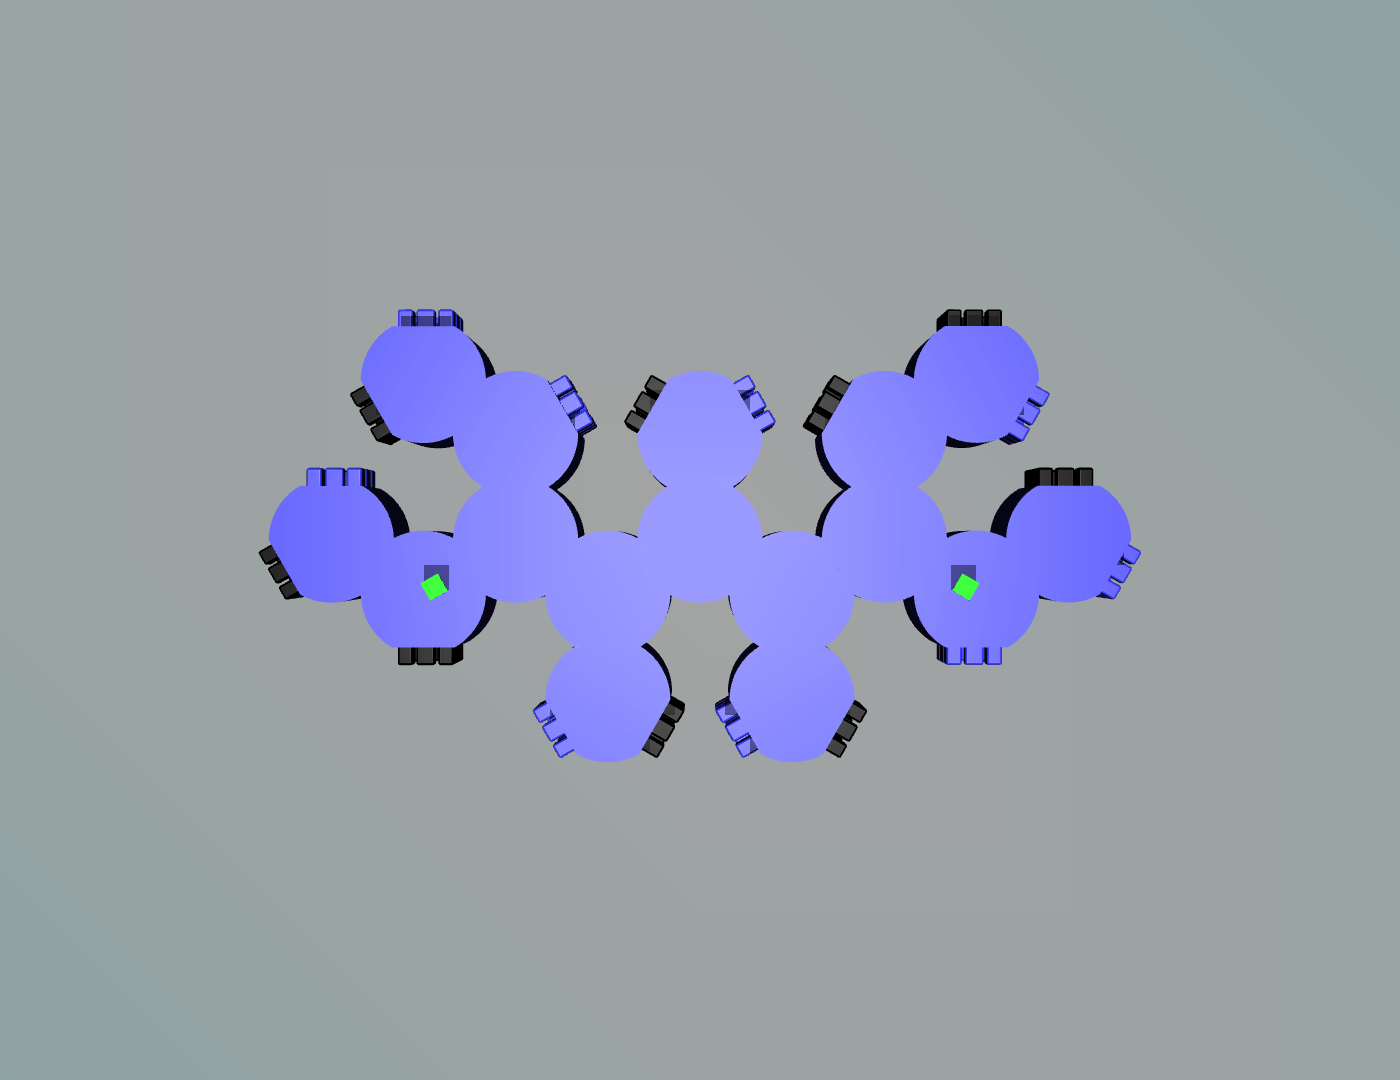
\includegraphics[width=\linewidth]{phermone_attracting_evolved_morph.png}
        \caption{Evolved morphology in the attractive configuration.}
        \label{fig:old-evolved-morphology-attractive}
    \end{subfigure}
    \par\vspace{0.6em}
    \begin{subfigure}[b]{\linewidth}
        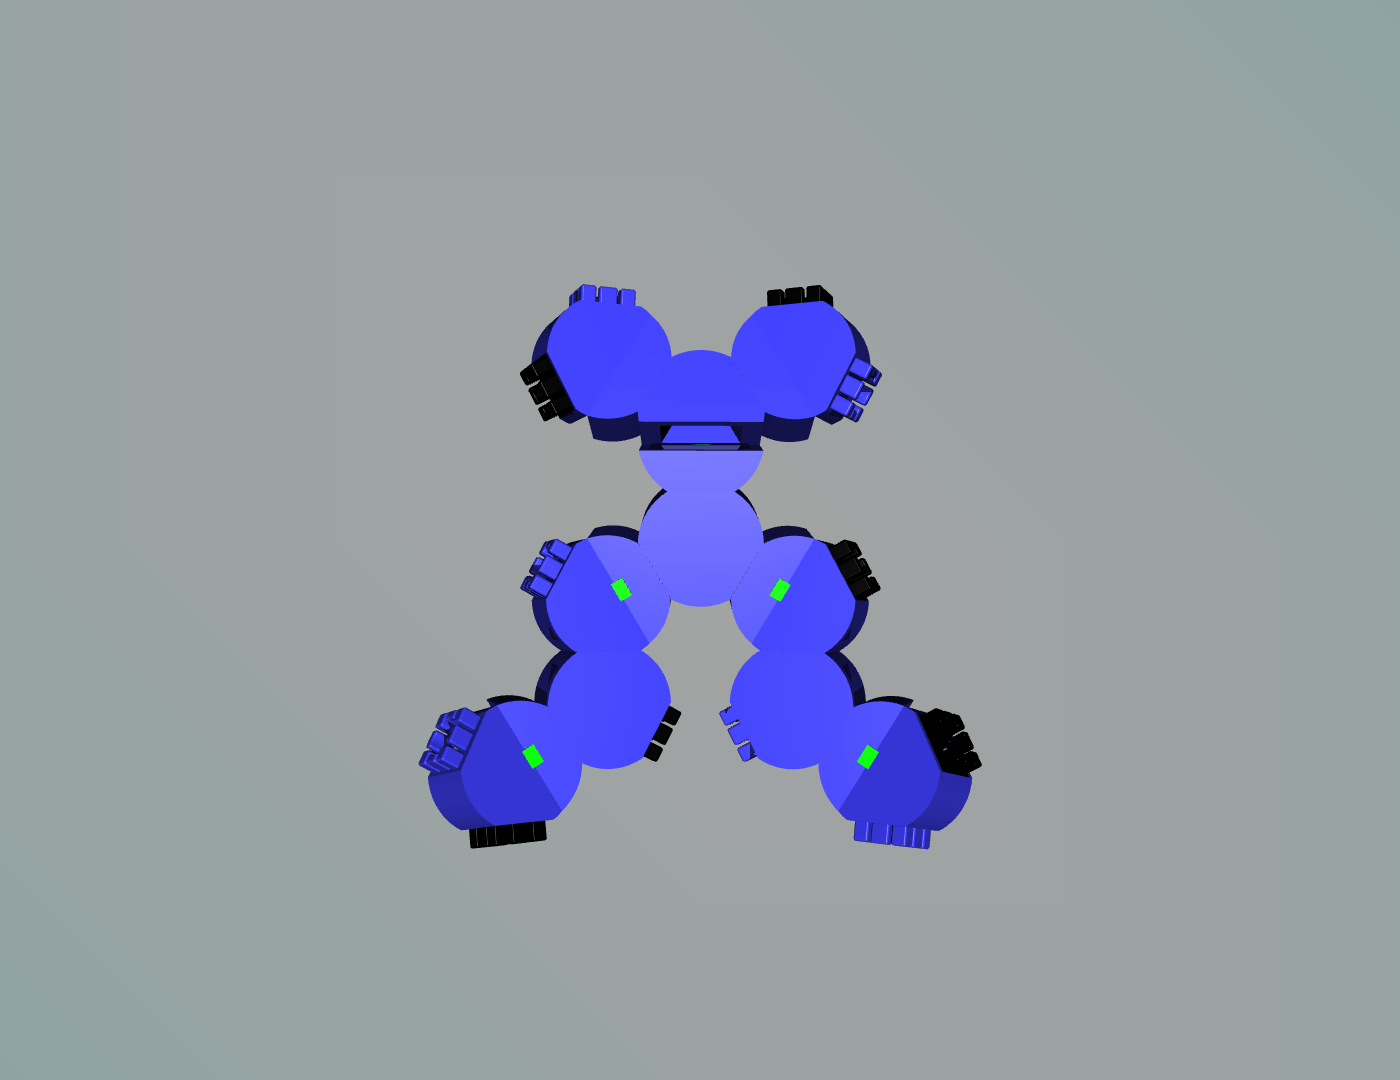
\includegraphics[width=\linewidth]{Phermone_repelling_evolved_morph.png}
        \caption{Evolved morphology in the repulsive configuration.}
        \label{fig:old-evolved-morphology-repulsive}
    \end{subfigure}
    \caption{Evolved morphologies in the attractive and repulsive configurations, resulted from few generation runs}
    \label{fig:old-evolved-morphology-both}
\end{figure}

\subsection{Single-Seed Results}
Every result in Chapter~\ref{ch:results} comes from a single random seed per configuration. Section~\ref{sec:rl-vs-random} shows outcomes that depend on which metric is read and at which point in the run, and without independent seeds it is not possible to say how much of that pattern would replicate versus reflect this particular run's own random draws.

\section{Future Work}

\subsection{Extended and Multi-Seed Evolutionary Runs}
Two extensions follow directly from the results in Chapter~\ref{ch:results}:
\begin{itemize}
    \item \textbf{Longer runs.} Hypervolume was still visibly rising at the end of the 300-generation run in every configuration reported (Section~\ref{sec:convergence-hv}), so extending the number of generations further would help establish whether the population is approaching a steady state or would continue improving substantially beyond the budget used here.
    \item \textbf{Multi-seed comparison.} The RL-versus-standard comparison (Section~\ref{sec:rl-vs-random}) should be repeated with multiple independent seeds per arm and, ideally, at the same generation budget as the main reported runs, since a single seed cannot distinguish a genuine algorithmic difference from run-to-run variation, and the current comparison and the longer diagnostic run were not conducted at matched generation budgets.
\end{itemize}

\subsection{RL Policy Improvements}
On the RL policy itself, the most promising direction identified in Section~\ref{sec:rl-diagnostics} is giving less-sampled action types (in particular the two crossover operators) a more reliable reward or advantage estimate, for example through per-action-type reward normalisation, rather than pooling all action types into a single running estimate. Further useful studies include ablations of the shared actor-critic encoder against separate actor/critic encoders, and sensitivity of training to the entropy-decay schedule.

\subsection{Physical Validation on Real Hardware}
Beyond the RL redesign, the best evolved designs should be checked on real Roblet units, to test the digital twin's assumptions about folding, connector placement, magnetic torque and light-sensitive joints, and to assess directly whether elongated repulsive-configuration morphologies of the kind flagged in Section~\ref{sec:limitations} are physically buildable. Together, these studies would show whether the learned policy contributes a genuine, reproducible advantage over random variation once the current reward and generation-budget limitations are addressed, and whether the simulated light responses and evolved morphologies transfer to physical hardware.


%%% List of references starts here.
\renewcommand{\bibname}{References}
\addcontentsline{toc}{chapter}{REFERENCES}
\bibliographystyle{unsrt}
\bibliography{Bibliography_uRL}

\chapter*{Use of AI}
\addcontentsline{toc}{chapter}{Use of AI}
AI tools were used for text rephrasing and code generation. They were not used for ideation, analysis, or the generation of any figures or results. The use of AI tools was limited to improving the clarity and presentation of the report, and all content was reviewed and verified by the author.

% ------------------------------------------------------------------
% APPENDICES (not marked, not counted in the page limit - Guidelines.md:
% "should not be used to simply keep the main report within the page
% limit"; only put things here a reader does NOT need for the main
% argument to make sense).
% ------------------------------------------------------------------
\appendix

\chapter{Glossary of Abbreviations}
\begin{tabular}{ll}
\textbf{EA} & Evolutionary algorithm \\
\textbf{GNN} & Graph neural network \\
\textbf{HV} & Hypervolume \\
\textbf{MJCF} & MuJoCo model format \\
\textbf{MOO} & Multi-objective optimisation \\
\textbf{NSGA-III} & Non-dominated Sorting Genetic Algorithm III \\
\textbf{PPO} & Proximal policy optimisation \\
\textbf{RL} & Reinforcement learning \\
\end{tabular}

\chapter{Repository Structure and Reproduction Instructions}
\label{app:reproduce}
This appendix is written for a future student or examiner who wants to re-run the simulation and evolutionary optimisation environment described in Chapter~\ref{ch:methodology}, rather than only read about it. Section~\ref{app:layout} maps the repository; Section~\ref{app:install} lists the exact software versions used; Section~\ref{app:running} explains how to launch a run, resume one, and reproduce a single evolved individual in isolation; Section~\ref{app:algo} tabulates the PPO and NSGA-III algorithm configuration in full, as the aspects of the pipeline that are this project's own contribution; and Section~\ref{app:params} gives the complete physical parameter reference that Table~\ref{tab:sim-params} in Chapter~\ref{ch:methodology} summarises.

\section{Repository Layout}
\label{app:layout}
The repository is organised into the following areas:
\begin{itemize}
    \item \texttt{src/} -- the simulation (\texttt{roblet\_simulator.py}), genotype grammar (\texttt{roblet\_grammar.py}), objective functions (\texttt{objectives\_api.py}, \texttt{entropy\_api.py}), reinforcement-learning policy (\texttt{rl\_api.py}), multi-objective loop (\texttt{moo\_api.py}), plotting code (\texttt{plotting\_api.py}), and the evolutionary-run entry point (\texttt{main.py}).
    \item \texttt{helper\_scripts/} -- the MJCF/XML generator (\texttt{mjcf\_generator.py}) and result-visualisation utilities.
    \item \texttt{graphs/} -- input graph descriptions.
    \item \texttt{models/} -- generated MJCF models.
    \item \texttt{output/} -- run outputs (checkpoints, logs, per-generation JSON and plots).
\end{itemize}

\section{Software Environment and Installation}
\label{app:install}
Dependency management is via \texttt{pyproject.toml} and its resolved lock file \texttt{uv.lock} (there is no separate \texttt{requirements.txt} or \texttt{environment.yml}); installation is therefore a single \texttt{uv sync} command run from the repository root, which creates a virtual environment matching Table~\ref{tab:software-versions} exactly. \texttt{gymnasium} and \texttt{stable-baselines3} are declared dependencies but are not used by the evolutionary loop itself; the PPO actor-critic is a hand-written Graph Transformer implementation in \texttt{src/rl\_api.py}, not an \texttt{stable\_baselines3} policy, and a future reader should not assume otherwise from the dependency list alone.

\begin{table}[htbp]
\centering
\footnotesize
\caption{Exact software versions resolved by \texttt{uv.lock} at the time the reported results were produced.}
\label{tab:software-versions}
\begin{tabular}{@{}ll@{}}
\toprule
\textbf{Package} & \textbf{Version} \\
\midrule
Python & 3.14.3 \\
mujoco & 3.10.0 \\
numpy & 2.5.0 \\
scipy & 1.18.0 \\
networkx & 3.6.1 \\
pymoo & 0.6.2 \\
torch & 2.13.0 \\
torch-geometric & 2.8.0.post1 \\
\bottomrule
\end{tabular}
\end{table}

\section{Running the Evolutionary Pipeline}
\label{app:running}
The evolutionary loop is launched with \texttt{python src/main.py}; it takes no command-line arguments, and every run parameter is instead a module-level constant near the top of that file (Table~\ref{tab:run-config}). A student wishing to reproduce or extend a specific reported result must set these constants to match the configuration stated in Section~\ref{sec:evo-learning} (or in the specific output directory's own saved logs, since \texttt{N\_GENERATIONS} in particular has been changed between runs and the current source value is not necessarily the one used for every reported figure).

\begin{table}[htbp]
\centering
\footnotesize
\caption{Key run-configuration constants, all set at the top of \texttt{src/main.py}.}
\label{tab:run-config}
\begin{tabular}{@{}p{5.2cm}p{8.4cm}@{}}
\toprule
\textbf{Constant} & \textbf{Meaning} \\
\midrule
\texttt{POP\_SIZE} & Population size (30 for every reported run). \\
\texttt{N\_GENERATIONS} & Number of generations; varies between reported runs -- check the target output directory's own logs rather than the current source default. \\
\texttt{SIM\_SECONDS} & Locomotion rollout duration in seconds (7 for every reported run). \\
\texttt{SEED} & Random seed for Sobol-sampling the initial population on a fresh run (42 for every reported run); a resumed run instead continues the RNG state stored in its checkpoint. \\
\texttt{RL\_ASSISTED\_GENETIC\_OPERATIONS} & \texttt{True} for the PPO-guided arm, \texttt{False} for the uniform-random baseline arm (Section~\ref{sec:evo-learning}). \\
\texttt{PHEROMONE\_RESPONSE\_TYPE} & \texttt{"attractive"} or \texttt{"repulsive"} (Section~\ref{sec:evo-learning}). \\
\bottomrule
\end{tabular}
\end{table}

Each generation proceeds as: population pool $\rightarrow$ \texttt{mjcf\_generator.build\_assembly} (per-individual MJCF/XML) $\rightarrow$ parallel headless MuJoCo evaluation in separate operating-system processes $\rightarrow$ \texttt{objectives\_api} (reads each individual's \texttt{stats.json}) $\rightarrow$ RL-assisted or random-baseline breeding $\rightarrow$ NSGA-III survival (\texttt{moo\_api}) $\rightarrow$ \texttt{plotting\_api} (plots and summary JSON) $\rightarrow$ checkpoint save. 
If a run is interrupted, re-issuing the same \texttt{python src/main.py} command resumes automatically from \\ \texttt{output/.../checkpoint.pt} with no additional flag; the output directory name itself encodes the run configuration, e.g. \texttt{output/evolution\_run} (RL-assisted, attractive), \texttt{output/evolution\_run\_norl} (random baseline), with a \texttt{\_repulsive} suffix appended for the repulsive configuration.

A single evolved individual can also be re-simulated in isolation, without running the full evolutionary loop, via the standalone command-line interface in \\ \texttt{src/roblet\_simulator.py} (e.g. \texttt{-m} to point at a specific MJCF model, \texttt{-o} to set the output/stats path, \texttt{-{}-b\_values} to repeat the field sweep, \texttt{-{}-light\_tests} to run the pheromone reaction-primitive protocol, and \\ \texttt{-{}-capture\_video}/\texttt{-{}-capture\_img}/\texttt{-{}-capture\_gif} to render the result). This is the most direct route for a future student who wants to inspect or validate one specific evolved morphology from a reported run.

\section{Algorithm Hyperparameters}
\label{app:algo}
The PPO-guided actor-critic (Section~\ref{sec:rl-actor-critic}) and the NSGA-III environmental selection (Section~\ref{sec:evo-learning}) are the two algorithmic components original to this project; their exact configuration is tabulated here in full, since this level of detail would interrupt the narrative in Chapter~\ref{ch:methodology} but is needed to reproduce a run exactly.

\begin{table}[htbp]
\centering
\footnotesize
\caption{PPO actor-critic hyperparameters. The Graph Transformer encoder architecture is shared between the actor and critic (separate weights, no parameter sharing); the optimisation hyperparameters are \texttt{PPOTrainer}'s constructor defaults as used, unmodified, by every reported run.}
\label{tab:rl-hyperparams-appendix}
\begin{tabular}{@{}p{6.4cm}p{7.4cm}@{}}
\toprule
\multicolumn{2}{@{}l}{\textit{Graph Transformer encoder (actor \& critic, separate weights)}} \\
\addlinespace[2pt]
Node feature dimension & 9 \\
Hidden dimension & 32 \\
Transformer blocks & 2 \\
Attention heads per block & 4 \\
Attention type & TransformerConv \citep{shi2020masked}, gated residual \\
Attention dropout & 0.1 \\
Feed-forward expansion & $2\times$ hidden, GELU \\
Cross-attention heads (actor, parent$_a$/parent$_b$ fusion) & 4 \\
Graph readout & Global mean pooling \\
\addlinespace[4pt]
\multicolumn{2}{@{}l}{\textit{PPO optimisation}} \\
\addlinespace[2pt]
Optimizer & Adam (separate actor/critic instances) \\
Learning rate & $3\times10^{-4}$ \\
Clip ratio $\epsilon$ & 0.2 \\
Entropy coefficient & Decays from $0.05$ to $0.02$, rate $0.995$ per update (Section~\ref{sec:rl-actor-critic}) \\
Value loss coefficient & 0.5 \\
PPO epochs per update & 4 \\
Gradient clipping & None \\
Advantage & $A = r - V(s)$, standardised per update \\
Discount / GAE & Not applicable (single-step contextual bandit) \\
\addlinespace[4pt]
\multicolumn{2}{@{}l}{\textit{Rollout and reward}} \\
\addlinespace[2pt]
Update frequency & Once per generation \\
Transitions per update & $n_{\text{offspring}}$ (= population size) \\
Action space & 10 grammar-legal actions (Table~\ref{tab:action-space-appendix}) \\
Reward & $r$ (Eq.~\ref{eq:reward-appendix}) \\
Collision/instability penalty & None -- excluded entirely from the reward stream rather than penalised (Eq.~\ref{eq:reward-appendix}, Section~\ref{sec:rl-actor-critic}) \\
\bottomrule
\end{tabular}
\end{table}

\begin{table}[htbp]
\centering
\footnotesize
\caption{Per-node state representation. The state for one breeding decision is the ordered pair of parent half-genotypes $(G_a, G_b)$; each is a variable-size directed graph (2--20 nodes pre-mirror) encoded per node as a 9-dimensional feature vector before being passed through the Graph Transformer encoder.}
\label{tab:state-space-appendix}
\begin{tabular}{@{}cp{4cm}p{7cm}@{}}
\toprule
\textbf{Idx} & \textbf{Feature} & \textbf{Definition} \\
\midrule
1--3 & Module type (one-hot) & \{rigid, mountain-fold, valley-fold\} \\
4 & Hinge angle & $\theta_v / 45^{\circ}$ \\
5 & Depth & $\min(\text{depth}_v, 10) / 10$ \\
6 & Free-port fraction & $|\text{free ports of } v| / 3$ \\
7 & Is root & 1 if $v = m_1$, else 0 \\
8 & Light-sensitive & 1 if $v$ carries the sensor, else 0 \\
9 & Light hinge angle & $\theta_{light,v} / 45^{\circ}$ (0 if not light-sensitive) \\
\bottomrule
\end{tabular}
\end{table}

\begin{table}[htbp]
\centering
\footnotesize
\caption{Action space: 10 grammar-legal actions, hierarchically sampled from one actor forward pass (action type $\rightarrow$ target node(s) $\rightarrow$ any parameters), each stage masked to legal choices only (Section~\ref{sec:evo-learning}'s grammar). The first eight are single-graph mutations acting on $G_a$ only; the last two are two-graph crossover operators.}
\label{tab:action-space-appendix}
\begin{tabular}{@{}p{3.6cm}p{4.6cm}p{5.6cm}@{}}
\toprule
\textbf{Action} & \textbf{Target(s)} & \textbf{Parameters} \\
\midrule
Add Node & Growable port on a node in $G_a$ & Port, fold type, hinge angle (if foldable) \\
Delete Node & Leaf node in $G_a$ & --- \\
Prune Subtree & Non-root node in $G_a$ & --- \\
Mutate Fold Type & Non-root node in $G_a$ & New fold type (categorical, 3-way) \\
Mutate Hinge Angle & Foldable node in $G_a$ & New $\theta_i$ (Gaussian, broadcast to all foldable modules) \\
Reconnect Port & Node in $G_a$ & Old port, new port (categorical, 3-way each) \\
Toggle Light Sensor & Foldable node in $G_a$ & --- \\
Mutate Light Hinge Angle & Light-sensitive node in $G_a$ & New $\theta_{light}$ (Gaussian, broadcast to all light-sensitive modules) \\
Graft Subtree & Host node in $G_a$ + donor root in $G_b$ & --- \\
Swap Subtrees & One node in $G_a$ + one node in $G_b$ & --- \\
\bottomrule
\end{tabular}
\end{table}

The reward for one breeding decision is the mean per-child improvement in scalarised fitness over its own parent. Collision and instability outcomes are excluded from the reward stream entirely rather than penalised: if the collision gate cannot find a single geometrically valid child after $N_{\text{attempts}}$ retries, or a child's simulated rollout is unstable or fails outright, no reward is recorded for that decision at all:
\begin{align}
r &= \frac{1}{|C|}\sum_{i \in C} \Delta_i \label{eq:reward-appendix} \\
\Delta_i &= \mathrm{scalarize}(f_{c_i}) - \mathrm{scalarize}(f_{p_i}) \\
\mathrm{scalarize}(f) &= \frac{1}{|\mathcal{A}|}\sum_{n \in \mathcal{A}} \hat f_n \\
\hat f_n &=
\begin{cases}
(f_n - f_n^{-}) / (f_n^{+} - f_n^{-}) & n \text{ maximised} \\
1 - (f_n - f_n^{-}) / (f_n^{+} - f_n^{-}) & n \text{ minimised}
\end{cases} \notag
\end{align}
where $C$ is the set of children of this decision (one child for a mutation or Graft Subtree; two, each scored against its own parent $p_i$, for Swap Subtrees); $f_n^{-}, f_n^{+}$ are the running observed minimum/maximum of objective $n$ over every individual scored so far in the run (online min-max normalisation); and $\mathcal{A} \subseteq \{f_1,\ldots,f_4\}$ restricts the average to objectives that have shown nonzero variation so far.

\begin{table}[htbp]
\centering
\footnotesize
\caption{NSGA-III environmental selection configuration (Section~\ref{sec:evo-learning}).}
\label{tab:nsga3-appendix}
\begin{tabular}{@{}p{5.2cm}p{8.8cm}@{}}
\toprule
\textbf{Setting} & \textbf{Value} \\
\midrule
Objectives & 4 ($f_1$--$f_4$, Eq.~\ref{eq:objectives}); all converted to minimisation form for pymoo \\
Reference directions & Das--Dennis, partition count auto-derived from population size (not fixed), so niching resolution scales with population \\
Feasibility handling & Structural validity enforced by construction (grammar masking, mirroring, collision gate); simulation success/failure recorded as a separate infeasibility flag \\
Elitism & Best individuals found so far retained explicitly across generations \\
Initial population & Sobol quasi-random sequence, scrambled, seeded from \texttt{SEED} \\
\bottomrule
\end{tabular}
\end{table}

\section{Full Physical Simulation Parameter Reference}
\label{app:params}
Table~\ref{tab:parts-appendix} gives the mass and bounding-box dimensions of each of the six moulded part types, as exported from the Fusion 360 CAD assembly; these are the source values converted into the per-part masses used by the MuJoCo digital twin (Section~\ref{sec:digital-twin}). Only mass and inertia are read from this CAD export at simulation-build time -- the body-local centre-of-mass offset used to position each part in the MJCF is a separately fitted value consistent with the CAD assembly, not a value read directly out of the export file, and a future reader extending this pipeline to a new part should not assume otherwise.

\begin{table}[htbp]
\centering
\footnotesize
\caption{Mass and bounding-box dimensions of each moulded part type, from the Fusion 360 CAD mass-property export. ``Fold-hinge base/link'' are the two halves of a foldable module's hinge; ``Rigid body'' is the non-foldable module shell; the three connector variants correspond to the three port types.}
\label{tab:parts-appendix}
\begin{tabular}{@{}lp{2cm}p{5.4cm}@{}}
\toprule
\textbf{Part (source mesh)} & \textbf{Mass} & \textbf{Bounding box (L $\times$ W $\times$ H)} \\
\midrule
Fold-hinge base (\texttt{BodyFoldedSide1.stl}) & 105 mg & $10.58 \times 10.33 \times 10.94$ mm \\
Fold-hinge link (\texttt{BodyFoldedSide2.stl}) & 91 mg & $9.28 \times 8.93 \times 10.73$ mm \\
Rigid body (\texttt{Body.stl}) & 196 mg & $11.62 \times 11.39 \times 10.94$ mm \\
Connector A (\texttt{SGA.stl}) & 41 mg & $6.99 \times 5.24 \times 6.50$ mm \\
Connector B (\texttt{SGB.stl}) & 43 mg & $6.31 \times 6.65 \times 6.26$ mm \\
Connector C (\texttt{SGX.stl}) & 67 mg & $6.70 \times 6.65 \times 6.56$ mm \\
Magnet (\texttt{Magnet.stl}) & 47.1 mg & $2\,\mathrm{mm}$ diameter $\times\ 2\,\mathrm{mm}$ height (cylinder) \\
\bottomrule
\end{tabular}
\end{table}

The remaining geometric constants needed to reassemble these parts into the MJCF model are: inter-module spacing along the parent-child axis, $8.5\,\mathrm{mm}$; fold-hinge $z$-offsets of $0.5\,\mathrm{mm}$ (valley) and $-5.5\,\mathrm{mm}$ (mountain) from the module origin; and connector-mount $z$-offsets of $1.03\,\mathrm{mm}$ (port 1), $1.10\,\mathrm{mm}$ (ports 2/3, foldable module) and $1.47\,\mathrm{mm}$ (ports 2/3, rigid module). The genotype's own design-variable bounds (Section~\ref{sec:evo-learning}) are: module count 2--20 per evolved half-genotype (2--40 after mirroring), and hinge/light-hinge angle 0\textdegree--45\textdegree, both enforced by clipping during mutation and by the sampling range used to construct the initial population.



\end{document}
% ----------------------------------------------------------------
